%% LaTeX Paper Template, Flip Tanedo (flip.tanedo@ucr.edu)
%% GitHub: https://github.com/fliptanedo/paper-template-2022

\documentclass[12pt]{article}

%!TEX root = paper.tex
%% FLIP’S PREAMBLE; 
%% Use FlipAdditionalHeader for project-specific packages & macros

% \pdfoutput=1 % for JHEP

%%%%%%%%%%%%%%%%%%%%%%%%%%
%%%  COMMON PACKAGES  %%%%
%%%%%%%%%%%%%%%%%%%%%%%%%%

\usepackage{amsmath}
\usepackage{amssymb}
\usepackage{amsfonts}
\usepackage{graphicx}
\usepackage[utf8]{inputenc}     % inspire bibs
\usepackage{aas_macros}				  % ads bibs
\usepackage{bm}                 % \boldsymbol
\usepackage{amsthm}
\usepackage{microtype}

%%%%%%%%%%%%%%%%%%%%%%%%%%%
%%%  UNUSUAL PACKAGES  %%%%
%%%%%%%%%%%%%%%%%%%%%%%%%%%

%% MATH AND PHYSICS SYMBOLS
%% ------------------------
\usepackage{slashed}				% \slashed{k}
\usepackage{mathrsfs}				% Weinberg-esque letters
\usepackage{bbm}					  % \mathbbm{1} conflict: XeLaTeX 
\usepackage{cancel}					
\usepackage[normalem]{ulem} % for \sout
\usepackage{youngtab}	    	% Young Tableaux

%% CONTENT FORMAT AND DESIGN
%% -------------------------
\usepackage[dvipsnames]{xcolor}
\usepackage[hang,flushmargin]{footmisc} % no footnote indent

\usepackage{fancyhdr}		% preprint number
\usepackage{lipsum}			% block of text 
\usepackage{framed}			% boxed remarks / Next time: use mdframed
                        % https://github.com/marcodaniel/mdframed/blob/master/mdframed.pdf
\usepackage{subcaption}	% subfigures
\usepackage{cite}			  % group cites
\usepackage{xspace}			% macro spacing


%% TABLES IN LaTeX
%% ---------------
\usepackage{booktabs}		% professional tables
\usepackage{nicefrac}		% fractions in tables,
\usepackage{multirow}		% multirow elements in a table
\usepackage{arydshln}		% dashed lines in arrays

%% ARRAY STRETCH: vertical spacing between rows
% \renewcommand{\arraystretch}{1.5} %% put this in main text

%% Other Packages and Notes
%% ------------------------
\usepackage[font=small]{caption} 	% caption font is small
\usepackage{float}         			  % for strict placement e.g. [H]


%%%%%%%%%%%%%%%%%%%%%%%%%%%%%%
%%%  DOCUMENT PROPERTIES  %%%%
%%%%%%%%%%%%%%%%%%%%%%%%%%%%%%

\usepackage[margin=2.5cm]{geometry} % margins
\graphicspath{{figures/}}			      % figure folder
\numberwithin{equation}{section}    % set equation numbering
% \usepackage{marginnote}             % for \marginnote{comment}
% \usepackage{mparhack}               % fix for \marginnote
% \usepackage{marginfix}              % fix for \marginnote
% \usepackage{adjustbox}              % to rescale elements



%% References in two columns, smaller
%% http://tex.stackexchange.com/questions/20758/
\usepackage{multicol}
\usepackage{etoolbox}
\usepackage{relsize}
\patchcmd{\thebibliography}
  {\list}
  {\begin{multicols}{2}\smaller\list}
  {}
  {}
\appto{\endthebibliography}{\end{multicols}}


% Change list spacing (instead of package paralist)
% from: http://en.wikibooks.org/wiki/LaTeX/List_Structures#Line_spacing
% alternative: enumitem package
\let\oldenumerate\enumerate
\renewcommand{\enumerate}{
  \oldenumerate
  \setlength{\itemsep}{4pt}
  \setlength{\parskip}{0pt}
  \setlength{\parsep}{0pt}
}

\let\olditemize\itemize
\renewcommand{\itemize}{
  \olditemize
  \setlength{\itemsep}{4pt}
  \setlength{\parskip}{0pt}
  \setlength{\parsep}{0pt}
}

%% FOR DRAFT EDITING AND DISCUSSION
\usepackage{lineno}
% \linenumbers          %% put this in main text


%%%%%%%%%%%%%%%%%%%%%%%%%%%
%%%  (RE)NEW COMMANDS  %%%%
%%%%%%%%%%%%%%%%%%%%%%%%%%%

%% FOR `NOT SHOUTING' CAPS (e.g. acronyms)
%% ---------------------------------------
\usepackage{scalefnt} 
\newcommand\acro[1]{{\footnotesize #1}}           % acronyms in footnote size


%% COMMON PHYSICS MACROS
%% ---------------------
\renewcommand{\tilde}{\widetilde}                 % tilde over characters
\renewcommand{\text}{\textnormal}	                % text in equations 
\renewcommand{\vec}[1]{\mathbf{#1}}               % vectors are boldface

%% Differential and differential/2pi
% \newcommand{\dbar}{d\mkern-6mu\mathchar'26}     % for d/2pi
\newcommand{\dbar}{d\mkern-6mu\mathchar'26\hspace{-.1em}}    
%% Best practice: Roman differential
\newcommand{\D}[1]{\ensuremath{\operatorname{d}\!{#1}}}
\newcommand{\Dbar}[1]{\operatorname{d}\mkern-10mu\mathchar'26\mkern-2mu{#1}}    % fixed spacing
\newcommand{\ket}[1]{\left|#1\right\rangle}       % <#1|
\newcommand{\bra}[1]{\left\langle#1\right|}       % |#1>
\newcommand*{\trans}{\mkern-1.5mu\mathsf{T}}      % transpose

%% COMMANDS FOR TEMPORARY COMMENTS
%% -------------------------------
\newcommand{\comment}[2]{\textcolor{red}{[\textbf{#1} #2]}}
\newcommand{\flip}[1]{{
	\color{green!50!black}
  \footnotesize
  [\textbf{\textsf{Flip}}: \textsf{#1}]
	}}


%% COMMANDS FOR TOP-MATTER
%% -----------------------
\newcommand{\email}[1]{\href{mailto:#1}{#1}}
\newenvironment{institutions}[1][2em]{\begin{list}{}{\setlength\leftmargin{#1}\setlength\rightmargin{#1}}\item[]}{\end{list}}


%% COMMANDS FOR LATEXDIFF
%% ----------------------
%% see http://bit.ly/1M74uwc
\providecommand{\DIFadd}[1]{{\protect\color{blue}#1}} %DIF PREAMBLE
\providecommand{\DIFdel}[1]{{\protect\color{red}\protect\scriptsize{#1}}}

%% REMARK: use latexdiff option --allow-spaces
%% for \frac, ref: http://bit.ly/1iFlujR
%% Errors with environments? https://tex.stackexchange.com/q/73224

%% USAGE: latexdiff draft.tex revision.tex > diff.tex

%%%%%%%%%%%%%%%%%%%%%
%%%  TITLE DATA  %%%%
%%%%%%%%%%%%%%%%%%%%%

%% PREPRINT NUMBER USING fancyhdr
%% Don't forget to set \thispagestyle{firststyle}
%% ----------------------------------------------
\renewcommand{\headrulewidth}{0pt} 	% no separator
\setlength{\headheight}{15pt} 		% min to avoid fancyhdr warning
\fancypagestyle{firststyle}{
	\rhead{\footnotesize%
	\texttt{\FlipTR}%
	}}

%% TOC overwrites fancyhdr, here's a fix
%% http://tex.stackexchange.com/questions/167828/
\usepackage{etoc}
\renewcommand{\etocaftertitlehook}{\pagestyle{plain}}
\renewcommand{\etocaftertochook}{\thispagestyle{firststyle}}			%% \usepackages
%!TEX root = paper.tex
%% Update the above with the appropriate root

%% Place additional project-specific macros, package calls here
%% These are called before FlipPreambleEnd.tex so that,
%% for example, they are called before hyperref


%% FIGURE SNIPPIT
% \begin{figure}[tb]
%     \centering
%     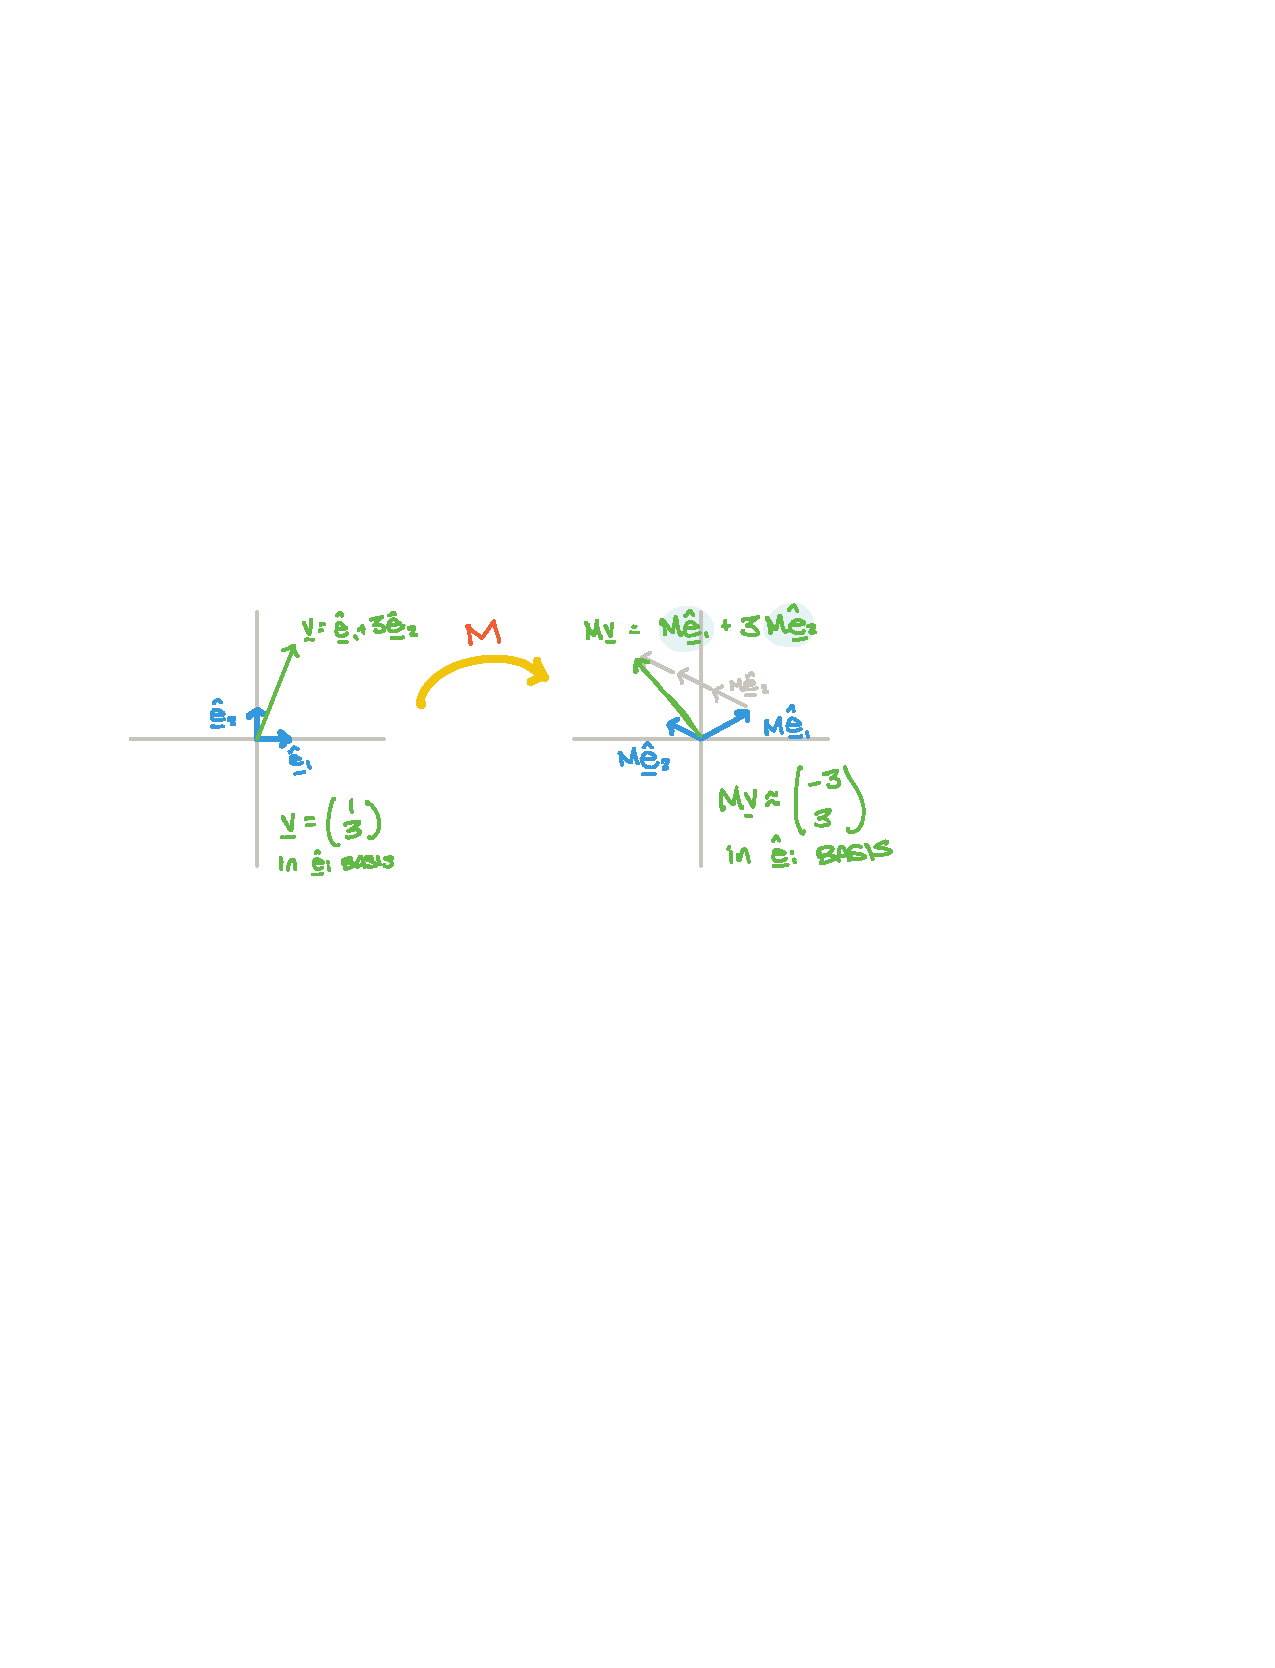
\includegraphics[width=.8\textwidth]{figures/maps_M.pdf}
%     \caption{.}
%     \label{fig:}
% \end{figure}

%% THEOREM ENVIRONMENTS


%% Because mdframed causes a bunch of warnings
%% https://tex.stackexchange.com/questions/64331/disable-warning-from-mdframed 
\usepackage{silence}
\WarningFilter{mdframed}{You got a bad break}
\WarningFilter{mdframed}{correct box splittet fails}



\newmdtheoremenv[
    skipabove=2em,
    skipbelow=2em,
    linewidth=5pt,
    linecolor=red!50!black,
    topline=false,
    rightline=false,
    bottomline=false
    ]{exercise}{Exercise}[section]


\newmdtheoremenv[
    skipabove=2em,
    skipbelow=2em,
    linewidth=5pt,
    linecolor=gray,
    topline=false,
    rightline=false,
    bottomline=false
    ]{example}{Example}[section]

\newmdtheoremenv[
    skipabove=2em,
    skipbelow=2em,
    linewidth=5pt,
    linecolor=blue,
    topline=false,
    rightline=false,
    bottomline=false
    ]{bigidea}{Key Idea}[section]
\newcommand{\bigidearef}{Key~Idea\xspace}
\newcommand{\bigidearefs}{Key~Ideas\xspace}

%% AMS Theorem version
% \newtheorem{exercise}{Exercise}[section]
% \newtheorem{example}{Example}[section]

%% Example: replace YourName with your name
\newcommand{\YourName}[1]{{	
	\color{blue!50!black}\footnotesize
	[\textbf{\textsf{YourName}}: \textsf{#1}]}}


\renewcommand{\tilde}{\widetilde}   % tilde over characters
\renewcommand{\vec}[1]{\mathbf{#1}} % vectors are boldface
\newcommand{\bas}[1]{\hat{\mathbf{#1}}} 	% basis vectors have hat
\newcommand{\row}[1]{\tilde{\mathbf{#1}}} 	% row vectors have tilde

% For matrices
\newcommand{\aij}[2]{^{#1}_{\phantom{#1}#2}}
\newcommand{\mat}[3]{#1\aij{#2}{#3}}
\newcommand{\pp}{\phantom{+}}
\newcommand{\inv}{^{-1}}


\usepackage{pifont}
	\newcommand{\cmark}{\ding{51}}%
	\newcommand{\xmark}{\ding{55}}%


%% COMMANDS FOR TEMPORARY COMMENTS
%% -------------------------------
\newcommand{\comment}[2]{\textcolor{red}{[\textbf{#1} #2]}}
\newcommand{\flip}[1]{{
	\color{green!50!black}
  \footnotesize
  [\textbf{\textsf{Flip}}: \textsf{#1}]
	}}

\newcommand{\correction}[2]{{
	\color{green!50!black}
  \footnotesize
  [\textbf{\textsf{Correction,~#1}}: \textsf{#2}]
	}}
 	%% Use this define additional macros
% %!TEX root = paper.tex
%% Update the above with the appropriate root


%% LISTINGS PACKAGE
%% https://www.overleaf.com/learn/latex/Code_listing
%% https://tex.stackexchange.com/a/350242
\usepackage{xcolor}
\usepackage[most]{tcolorbox}
\usepackage{listings}

\definecolor{white}{rgb}{1,1,1}
\definecolor{mygreen}{rgb}{0,0.4,0}
\definecolor{light_gray}{rgb}{0.97,0.97,0.97}
\definecolor{mykey}{rgb}{0.117,0.403,0.713}

\tcbuselibrary{listings}
\newlength\inwd
\setlength\inwd{1.3cm}

\newcounter{ipythcntr}
\renewcommand{\theipythcntr}{\texttt{[\arabic{ipythcntr}]}}

\newtcblisting{pyin}[1][]{%
  sharp corners,
  enlarge left by=\inwd,
  width=\linewidth-\inwd,
  enhanced,
  boxrule=0pt,
  colback=light_gray,
  listing only,
  top=0pt,
  bottom=0pt,
  overlay={
    \node[
      anchor=north east,
      text width=\inwd,
      font=\footnotesize\ttfamily\color{mykey},
      inner ysep=2mm,
      inner xsep=0pt,
      outer sep=0pt
      ] 
      at (frame.north west)
      {\refstepcounter{ipythcntr}\label{#1}In \theipythcntr:};
  }
  listing engine=listing,
  listing options={
    aboveskip=1pt,
    belowskip=1pt,
    basicstyle=\footnotesize\ttfamily,
    language=Python,
    keywordstyle=\color{mykey},
    showstringspaces=false,
    stringstyle=\color{mygreen}
  },
}
\newtcblisting{pyprint}{
  sharp corners,
  enlarge left by=\inwd,
  width=\linewidth-\inwd,
  enhanced,
  boxrule=0pt,
  colback=white,
  listing only,
  top=0pt,
  bottom=0pt,
  overlay={
    \node[
      anchor=north east,
      text width=\inwd,
      font=\footnotesize\ttfamily\color{mykey},
      inner ysep=2mm,
      inner xsep=0pt,
      outer sep=0pt
      ] 
      at (frame.north west)
      {};
  }
  listing engine=listing,
  listing options={
      aboveskip=1pt,
      belowskip=1pt,
      basicstyle=\footnotesize\ttfamily,
      language=Python,
      keywordstyle=\color{mykey},
      showstringspaces=false,
      stringstyle=\color{mygreen}
    },
}
\newtcblisting{pyout}[1][\theipythcntr]{
  sharp corners,
  enlarge left by=\inwd,
  width=\linewidth-\inwd,
  enhanced,
  boxrule=0pt,
  colback=white,
  listing only,
  top=0pt,
  bottom=0pt,
  overlay={
    \node[
      anchor=north east,
      text width=\inwd,
      font=\footnotesize\ttfamily\color{mykey},
      inner ysep=2mm,
      inner xsep=0pt,
      outer sep=0pt
      ] 
      at (frame.north west)
      {\setcounter{ipythcntr}{\value{ipythcntr}}Out#1:};
  }
  listing engine=listing,
  listing options={
      aboveskip=1pt,
      belowskip=1pt,
      basicstyle=\footnotesize\ttfamily,
      language=Python,
      keywordstyle=\color{mykey},
      showstringspaces=false,
      stringstyle=\color{mygreen}
    },
}





%!TEX root = paper.tex
%% These are packages that need to be called at the end of the preamble 
%% or else they may lead to potential package conflicts.

%%%%%%%%%%%%%%%%%%%
%%%  HYPERREF  %%%%
%%%%%%%%%%%%%%%%%%%

%% This package has to be at the end; can lead to conflicts
\usepackage[
	colorlinks=true,
	citecolor=green!50!black,
	linkcolor=NavyBlue!75!black,
	urlcolor=green!50!black,
	hypertexnames=false]{hyperref}

%%%%%%%%%%%%%%%%%%%%%%%%%%%%%%%%%%%%%%%%
%%%  Must be called after HYPERREF  %%%%
%%%%%%%%%%%%%%%%%%%%%%%%%%%%%%%%%%%%%%%%


\usepackage{orcidlink}			% orcid ID icon; after hyperref
\usepackage{cleveref}
\crefformat{equation}{(#2#1#3)}	% strip eq.~ 
\crefrangeformat{equation}{(#3#1#4\,--\,#5#2#6)} % strip eqs.~			%% packages that have to be at the end
\begin{document}

\newcommand{\FlipTR}{UCR-TR-2023-FLIP-00X} % (pdfsync may fail on 1st page)
	\thispagestyle{firststyle} 	% TR#; otherwise use \thispagestyle{empty}


%%%%%%%%%%%%%%%%%%%%%%%%
%%%  FRONTMATTER    %%%%
%%%%%%%%%%%%%%%%%%%%%%%%

\begin{center}
    {\huge \textbf{Linear Algebra for Physicists} \par}
    \vskip .5cm
    %!TEX root = paper.tex
%% Update the above with the appropriate root

%% This is the author list
%% We separate it to keep the main file clean; this is
%% not the part of the document that gets updated often.

\newcommand{\authorA}{Flip Tanedo}
\newcommand{\emailA}{flip.tanedo@ucr.edu}
\newcommand{\orcidA}{0000-0003-4642-2199}
\newcommand{\institutionA}{
		Department of Physics \& Astronomy, 
	    University of  California, Riverside, 
	    \acro{CA} 92521}

\newcommand{\authorB}{Your Name}
\newcommand{\emailB}{your.name@ucr.edu}
\newcommand{\orcidB}{0000-0003-4642-2200}
\newcommand{\institutionB}{
		Department of Physics \& Astronomy, 
	    University of  California, Elsewhere, 
	    \acro{CA} 99999}

\newcommand{\authorC}{Tu Nombre}
\newcommand{\emailC}{tu.nombre@ucr.edu}
\newcommand{\orcidC}{0000-0003-4642-2201}
\newcommand{\institutionC}{
		Department of Physics \& Astronomy, 
	    University of  California, Elsewhere, 
	    \acro{CA} 99999}

	\textbf{\authorA}%$^{a}$,
	% \textbf{\authorB}$^{b}$,
	% and
	% \textbf{\authorC}$^{c}$, 
	\\ 
	\texttt{\footnotesize \email{\emailA}}~\orcidlink{\orcidA}%,
	% \texttt{\footnotesize \email{\emailB}}~\orcidlink{\orcidB},
	% \texttt{\footnotesize \email{\emailC}}~\orcidlink{\orcidC}

	\vspace{-.8em}
    \begin{institutions}[1.7cm]
    \footnotesize
    { 
    	% $^{a}$
    	\textit{\institutionA} 
    	% \\ $^{b}$ \textit{\institutionB} 
    	% \\ $^{c}$ \textit{\institutionC} 
	}    
    \end{institutions}


\end{center}

\begin{abstract}
\noindent 
Lecture notes for Physics 17, a course on linear algebra in preparation for upper-division undergraduate physics coursework at \acro{UC~R}iverside.
\end{abstract}




\small
\setcounter{tocdepth}{2}
\tableofcontents
\normalsize
%\clearpage


%%%%%%%%%%%%%%%%%%%%%
%%%  THE CONTENT  %%%
%%%%%%%%%%%%%%%%%%%%%

\section{Logistics}


\subsection{Two powerful questions}
At any time in this course, you should feel comfortable asking either of the following questions:
\begin{enumerate}
    \item Is it obvious that...?
    \item Why is this significant?
\end{enumerate}
The first question is the way to ask for on-the-spot clarification---I will either appreciate that I did not properly explain a subtle point, \emph{or} I will explain the intuition\footnote{Your sense of mathematical and physical intuition is incredibly valuable. This is one of the key traits that makes a physics training unique.} for why something should be obvious. The second question is a way to remind me that I may have \emph{lost sight of the forest for the trees}: I want this course to \emph{mathematically connect big ideas in physics}. Asking this question is a reminder that making those connections justifies the hard mathematical work we will put into the course.

\subsection{Exercises and Examples}
I have tried to insert exercises and examples in these notes. There are still far too few for sound pedagogy. If you really, really want to learn something, you \emph{have} to do exercises. Think of the examples as exercises with solutions---though they are not always written this way. Mull over the exercises: ask yourself why the problems are posed the way they are, challenge the statements to find the domain of validity, think of how one may extend those exercises to other applications. The exercises are a far better gauge of you learning than whether or not you have read a section of the notes. If you are confused reading the text in section 10, it is often the case that you should have been doing the exercises since section 5.


\subsection{Obvious-ness}
Finally, I want to comment on the word \emph{obvious}. I write this often. It is somewhat dangerous because it can come off as being arrogant: \emph{this is so obvious to me, if you do not understand you must be deficient}. This is never the reason why I use that word. Instead, the word \emph{obvious} serves a very practical purpose. The goal of this class is not just to be able to ``do stuff'' (e.g.~diagonalize a symmetric matrix), but to also build that intuition that comes from a deeper understanding how the mathematics works. In this sense, every time I write the word \emph{obvious} it is a flag: I am saying something that---with the proper perspective---should be self-evident. If it is not self-evident, then you should stop to interrogate why it is not self-evident. Most likely there is something where a change in perspective may (1) make it obvious, and (2) in so doing deepen your understanding of the subject. So when you see the word `obvious,' I want you to do a quick check to confirm whether or not the statement is indeed obvious. If it is not, then welcome the opportunity to learn.\footnote{There is, of course, the possibility that what I have written is \emph{not} obvious. For example, if I have made a typo... in which case, please let me know.}

\section{Motivation}

Here are three incredibly significant equations in physics:
\begin{align}
    \vec{F} &= m\vec{a}
    &
    R_{\mu\nu} - \frac{1}{2}Rg_{\mu\nu} 
    &= \frac{8\pi G_\text{N}}{c^4} T_{\mu\nu}
    &
    \hat H |\Psi\rangle 
    &= E |\Psi\rangle \ .
    \label{eq:three:equations}
\end{align}
These are Newton's force law, Einstein's field equations, and the Schr\"odinger equation. They govern classical physics, general relativity, and quantum theory. 


Each equation looks rather unique: they seem to each be speaking their own mathematical language. Newton's law is written with boldfaced vectorial quantities $\vec{F} = (F_x, F_y, F_z)^T$ that should look very familiar to any physics undergraduate. Einstein's equation has these funny $\mu$ and $\nu$ indices on every term---have you seen these before? Do they look intimidating? If you ever want to make your equations look ``technical'' and ``physicsy,'' you should dress them up with indices. The Schr\"odinger equation has no indices, but instead has these funny angle-brackety things... and that $\hat H$ looks suspicious. Where did $H$ get a hat, and what is the content of this equation other than $\hat H = E$?

\emph{Each of these equations turns out to be a ``vectorial'' equation.} Each one is actually shorthand for a number of equations. Newton's equation is shorthand for three equations, one for each component. Einstein's equation is shorthand for 16 equations, one for each combination of the indices $\mu$ and $\nu$ that run over four values\footnote{The four values are the three directions of space and one direction of time.}. The Schr\"odinger equation is shorthand for an \emph{infinite} number of equations, one for each allowed energy of a quantum system.

The mathematical formalism that unifies these different ideas (and notations) of `vector' is called linear algebra. It may sound humble: after all, ``linear'' systems are \emph{easy}, aren't they? Did we not just spend years of our lives learning fancy things like \emph{calculus} and \emph{differential equations} to deal with functions that are more complicated than \emph{lines}? In some sense, yes: linear algebra is about lines and planes in different numbers of dimensions.\footnote{On the other hand: a good chunk of the calculus that we do is also implicitly linear. Physicists often Taylor expand and keep only the $\mathcal O(\varepsilon)$ term. Integration boils down to summing trapezoids whose angley-bits are given by the first derivative of a function... the linear component.} However, linear algebra turns out to be far more richer than what you may be used to from high school. 

In this course we will see how the three equations in \eqref{eq:three:equations} are connected by the mathematics of linear algebra. We will dive into the different notation and shamelessly pass between $\vec{v}$, $v^i$, and $\ket{v}$ to describe the same abstract vector. We will connect to the mathematical description of \emph{symmetry} and see how it is an underlying theme in our descriptions of nature. And we will do all of this in a way that will make the instructors of the linear-algebra-for-mathematicians course and linear-algebra-for-engineers course vomit a little in disgust. Consider that one of privileges of being a physicist.


\section{Basics}

\subsection{Pre-conceptions}

If this were a mathematics course, then we would start by very carefully defining words like \emph{vector} and \emph{matrix}. As a physics student, you already have a working definition of these words. It is probably something like this:
%
\begin{quote}
A vector has a magnitude and a direction. We write a vector as an array of three numbers arranged in a column. A matrix is an array of nine numbers arranged in a $3\times 3$ block. There is a rule for how to apply (multiply) the matrix to the vector to produce a new vector.
\end{quote}

The problem is that you already know too much to learn linear algebra as a mathematics student. You have already seen the tip of the iceberg and so have preconceptions about what vectors are and how they work. You may remember from freshman mechanics that forces are vectors. So are momenta and velocities. You may also recall the idea of a force field---like the electric field---which is actually a whole bunch of vectors: one for each point in space. Examples of matrices are a little more subtle: you may recall that you can represent rotations as matrices. Speaking of rotations, there was another thing that showed up called the moment of inertia \emph{tensor}. It looked like a matrix, but we never called it the ``moment of inertia matrix.'' What the heck is a tensor, anyway?

And so, you see that starting this course like a mathematics course could cause trouble. The mathematics professor would start by defining a vector. That definition will say nothing about magnitudes or directions, and will not even say anything about arrays of numbers. That definition will clash with the hard-earned intuition that you built from your physics education thus far. It will be perplexing, and may make you feel rather unhappy. What do these mathematicians know, anyway? Or maybe its the physics that is wrong, or have we just completely misunderstood everything and we are just now noticing that we are hopelessly lost? We begin to spiral into a black hole of confusion.

\begin{quote}
Fortunately, \emph{this is not a mathematics course.}
\end{quote}

As a consequence, we will not give a rigorous definition of a vector. We start with a familiar definition of vectors and lay out which qualities are general, and which properties are specific. Then we will come to appreciate the approximation that ``\emph{everything is a vector}.'' So let us start with something comfortably familiar, even though it constitutes only the simplest example of a vector.

\subsection{Real Three-Vectors}

Let us write $\vec{v}$ to be a vector. This is a standard convention for writing a vector. In this course we will use a few different notations for vectors according to convenience. Notation is neither physics nor mathematics, it is simply a shorthand for a physical or mathematical idea. 

% At this point, you may wonder \emph{what is a vector, anyway?} Maybe a vector is a column with three numbers that represent coordinates in three-dimensional space:
In fact, let us focus on a particular type of vector: \textbf{real three-vectors}. These are the familiar vectors that we can write as a column of three numbers that effectively represent the coordinates in three-dimensional space:
\begin{align}
    \vec{v} = 
    \begin{pmatrix}
        x\\ y\\ z
    \end{pmatrix} \ ,
\end{align}
where $x$, $y$, and $z$ are real numbers. These numbers are called the \textbf{components} of the vector $\vec{v}$.

\begin{exercise}
There is something very perverse about this ``vector.'' The variable names $x$, $y$, and $z$ imply that $\vec{v}$ is something that physicists like to call a ``position vector.'' If you say this to a mathematician they will vomit. By the end of this course, you should appreciate why the notion of a position vector makes no sense. \emph{Hint:} You may have some intuition for this already: a velocity vector tells you about the instantaneous motion of a particle relative to its present position. Try to write the analogous statement for a ``position vector.\footnote{I am not a mathematician, but you see that even I have to write ``position vector'' in condescending quotation marks. In lecture I use even more condescending air quotes.}''
\label{ex:position:vector}
\end{exercise}

This three-dimensional space is called [three-dimensional] \textbf{real space} and we write it as $\RR ^3$. This is because a vector is an element of three-dimensional real space specified by \emph{three} real numbers. 

Three-dimensional real space is an example of a \textbf{vector space}, which is just a stupidly formal way of saying that it is where vectors live. Vectors are \emph{elements} of a vector space. A vector space is the set of all possible allowed vectors of a given type. For $\RR ^3$, the vector space is composed of all possible triplets of real numbers. 


\begin{example} It should be no surprise that we can imagine real two-dimensional space, $\RR ^2$. This is a vector space where each vector may be written as two real numbers. You can also imagine writing real four-dimensional space, $\RR ^2$, or complex two dimensional space, $\mathbbm{C}^2$. 
\end{example}

From the above example, you should have some intuition for what the \textbf{dimension} of a vector space means: the dimension counts how many numbers you need to specify a vector. For real vector spaces, $\RR ^d$, the dimension is the number $d$. We will always assume that $d$ is a positive integer.\footnote{The notion of a non-integer-dimensional space does show up occasionally. These do not even have to be particularly exotic: you can look up the dimension of a fractal.}

\subsection{Vectors and Numbers}

% We now make some general statements about vector spaces. These apply to all vector spaces, not just $\RR ^3$, but you can keep $\RR ^3$ in mind as we go over them. 

We should be clear that there are now two different kinds of objects: \emph{vectors} and \emph{numbers}. We will have all sorts of notation for vectors, but let us write them with a boldfaced Roman letter for now, e.g.~$\vec{v}$. We typically write numbers as lowercase italicized Roman letters like $a$ or sometimes Greek letters like $\alpha$. These two types of objects are similar, except vectors do not have a built-in definition for multiplication, see Table~\ref{table:vectors:numbers}.

\begin{table}
    \renewcommand{\arraystretch}{1.3} % spacing between rows
    \centering
    \begin{tabular}{ @{} lll @{} } \toprule % @{} removes space
         & Vectors & Numbers 
        \\ \hline
        Addition (commutative, associative) & \cmark & \cmark 
        \\
        Additive null element & $\vec{0}$ & 0
        \\
        Additive inverse element & $\vec{v} + (-\vec{v}) = 0$ & $a + (-a) = 0$
        \\
        Multiplication of two of these objects & \textcolor{red}{\xmark} & \cmark 
        \\
        Multiplication by a number (distributive) & \cmark & \cmark \,(same as above)
        \\
        Collection of all allowed objects (space) & vector space & field (``numbers'') 
        \\
        Example of a space & $\RR ^3$ & $\RR $
        \\ \bottomrule
    \end{tabular}
    \caption{
        What you can do with vectors compared to numbers. The glaring difference is that we cannot multiply two vectors. We will need to invent additional mathematical structure to define vector multiplication.
        \label{table:vectors:numbers}
  }
\end{table}

You already know everything there is to know about numbers.\footnote{Formally, what I mean by `number' is what mathematicians call a \textbf{field}. This simply means some objects where one can add, subtract, multiply, and divide as you would expect. This term is a little tedious for us because physicists usually mean something else when they say `field.' Usually we mean something like the electric field or the field associated with the Higgs boson.} Most relevant is that you can multiply numbers with each other (including division, the inverse of multiplication) and you can add them together (including subtraction). For the first part of this course, we will focus on real numbers, $\RR $. Later we will also allow for complex numbers, $\mathbbm{C}$. 

Like numbers, vectors can be added and subtracted. In fact, vector arithmetic turns out to be very similar to `number arithmetic.' However, unlike numbers, there is no obvious definition for vector multiplication. This leads to the idea of \emph{defining} functions for various kinds of vector multiplication. Linear algebra is the study of a particular class of these functions. The dot product, for example, which takes two vectors and returns a number, is something we have to ``make up'' and attach to a vector space.

% What about vectors? Vectors have the following properties: 
% \begin{enumerate}
%     \item You can add vectors. This assumes that they are in the same vector space. The sum of two vectors is also a vector in the same vector space. 
%     \item Vector addition is associative. This means that in the sum $\vec{v}+\vec{w}+\vec{u}$, it does not matter if you add $(\vec{v}+\vec{w})$ first and then add $\vec{u}$, or if you take $\vec{v}$ and then add it to $(\vec{w}+\vec{u})$. This is the kind of `obvious' property that we tend to take for granted.
%     \item Vector addition is commutative. $\vec{v}+\vec{w} = \vec{w}+\vec{v}$. This is also kind of obvious. But recall that matrix multiplication is not commutative.
%     \item There is a zero vector, $\vec{0}$, that does leaves any other vector unchanged under addition. $\vec{v}+\vec{0} = \vec{v}$. This should be totally obvious. I bet you even know what the components of $\vec{0}$ are.
%     \item There is an additive inverse (negative vectors). If $\vec{v}$ is a vector, then $-\vec{v}$ is a vector and satisfies $\vec{v}+(-\vec{v}) = \vec{0}$.
%     \item You can multiply vectors by numbers. This is called rescaling or scalar multiplication. All the usual properties of multiplication by numbers holds: associativity, commutivity, distributive law.
% \end{enumerate}
% \begin{example}
% The first property implies that once you have identified one vector in a vector space, $\vec{v}$, then you can immediately have an infinite number of vectors. This is because $2\vec{v} = \vec{v}+\vec{v}$ must also be a vector. Then $3\vec{v} = 2\vec{v}+\vec{v}$ must also be a vector. And so forth.
% \end{example}
% Let us go over a few of these properties.

\subsection{Notation: Indices}

One theme in this course is that we will repeatedly refine our notation to suit our needs. Let us introduce an \emph{index} notation where we write the components of vectors $\vec{v}$ and $\vec{w}$ as follows:
\begin{align}
    \vec{v}
    &=
    \begin{pmatrix}
        v^1 \\ v^2 \\ v^3
    \end{pmatrix}
    &
    \vec{w}
    &=
    \begin{pmatrix}
        w^1 \\ w^2 \\ w^3
    \end{pmatrix} \ .
\end{align}
We see that a boldfaced Roman letter, $u$, corresponds to a vector. The \emph{components} of the vector are $u^1$, $u^2$, $u^3$. The ``$x$-component'' of $\vec{u}$ is called $u^1$: we use the same letter as the vector, but italicized rather than boldfaced. The upper index is \emph{not} some kind of power, it simply means ``the first component.'' 

\begin{example}
If you see $\vec{s}$, this is understood to be a vector that has multiple components. If it is a three-vector, it has three components. If you see $s^2$, then this means that this is the \emph{second component} of the vector $\vec{s}$. The component of a vector is a number. 
\end{example}

You may worry that this notation introduces ambiguity. If we see $q^2$, is this the square of some number $q$, or is it the second component of some vector $\vec{q}$? The answer depends on context. You should avoid choosing variable names where there is ever the potential for ambiguity. If you have a vector that you call $\vec{q}$, then do not use the letter $q$ for anything else.


% \subsection{Notation: Indices again}

% We can express this using index notation. 
You know from $\RR ^3$ that you can add together any two vectors $\vec{v}$ and $\vec{w}$.
% 
Let us call this sum $\vec{u}$ so that $\vec{u}\equiv \vec{v}+\vec{w}$. Then we can succinctly write the components of $\vec{u}$ in one line:
\begin{align}
    u^i = v^i + w^i \ .
    \label{eq:u:v:plus:w:index}
\end{align}
The variable $i$ is called an \textbf{index}. What values does the index take? In this example, it is 
clear that \eqref{eq:u:v:plus:w:index} holds for $i=1,2,3$. That is, $i$ takes values from 1 to the dimension of the space. The typical convention is that we do not have to state the range of index values because it should be understood from the space itself. 

With that in mind, it should be clear that if $\vec{q}$ is the difference of two vectors, then the components of $\vec{q}$ may be succinctly written:
\begin{align}
\vec{q} &= \vec{v}-\vec{w}    
&
&\Leftrightarrow
&
q^i &= v^i - w^i \ .
\end{align}
In fact, as physicists we typically use the two statements above interchangeably. If you know the components of a vector, then you know the vector.



\subsection{Arithmetic and linear combinations}

All vector spaces allow addition and subtraction. This is defined component-wise. The sum of $\vec{v}$ and $\vec{w}$ is
\begin{align}
    \vec{v}+\vec{w} = 
    \begin{pmatrix}
        v^1 + w^1\\
        v^2 + w^2\\
        v^3 + w^3
    \end{pmatrix} \ .
\end{align}
What this means is that the \emph{sum} of two vectors is also a vector. That means that if $\vec{v}$ and $\vec{w}$ are vectors in $\RR ^3$, then $(\vec{v}+\vec{w})$ is a vector in $\RR ^3$. The components of the vector $(\vec{v}+\vec{w})$ are simply the sum of the components of $\vec{v}$ and $\vec{w}$. 
% 
A few formal properties that generalize to all vector spaces:
\begin{itemize}
    \item Vector addition is associative. This means that in the sum $\vec{v}+\vec{w}+\vec{u}$, it does not matter if you add $(\vec{v}+\vec{w})$ first and then add $\vec{u}$, or if you take $\vec{v}$ and then add it to $(\vec{w}+\vec{u})$. This is the kind of `obvious' property that we tend to take for granted.
    \item Vector addition is commutative. $\vec{v}+\vec{w} = \vec{w}+\vec{v}$. This is also kind of obvious. But recall that matrix multiplication is not commutative.
    \item There is a zero vector, $\vec{0}$, that does leaves any other vector unchanged under addition. $\vec{v}+\vec{0} = \vec{v}$. This should be totally obvious. The components of $\vec{0}$ are obviously all zero.
    \item There is an additive inverse (negative vectors). If $\vec{v}$ is a vector, then $-\vec{v}$ is a vector and satisfies $\vec{v}+(-\vec{v}) = \vec{0}$.
\end{itemize}
\begin{example}
The first property implies that once you have identified one vector in a vector space, $\vec{v}$, then you can immediately have an infinite number of vectors. This is because $2\vec{v} = \vec{v}+\vec{v}$ must also be a vector. Then $3\vec{v} = 2\vec{v}+\vec{v}$ must also be a vector. And so forth.
\end{example}

We get another type of operation ``for free'' with a vector space. This is called scalar multiplication or \emph{rescaling}.

% You can multiply vectors by numbers. This is called rescaling or scalar multiplication. All the usual properties of multiplication by numbers holds: associativity, commutivity, distributive law.









\subsection{Rescaling: multiplication by a number}

Another operation that exists in a vector space is rescaling: we multiply a vector by a number. 
Let $\alpha$ be a number. If you want to nitpick, let us restrict $\alpha$ to be a real number. If we have a vector $\vec{v}$ with components $v^i$, then $\alpha \vec{v}$ is also a vector.\footnote{``Also a vector'' means that it is also an element of the vector space; so $(\alpha\vec{v})$ is an element of $\RR ^3$ is $\vec{v}$ is an element of $\RR ^3$. } The components of $\alpha \vec{v}$ are
\begin{align}
    (\alpha v)^i = \alpha v^i \ ,
\end{align}
by which we mean
\begin{align}
    (\alpha\vec{v})
    =
    \begin{pmatrix}
        \alpha v^1 \\
        \alpha v^2 \\
        \alpha v^3 
    \end{pmatrix} \ .
\end{align}
The parenthesis on the left-hand side is sloppy notation to mean ``the vector that is the vector $\vec{v}$ rescaled by the number  $\alpha$.'' Another way of saying this is that there is a vector $\vec{w}\equiv \alpha\vec{v}$ whose components are $w^i = \alpha v^i$.

\begin{example}
Let us do one explicit example with numbers. Suppose the vectors $\vec{v}$ and $\vec{w}$ have components
\begin{align}
    \vec{v} &=
    \begin{pmatrix}
    \phantom{+}4.2\\
    -2.6\\
    \phantom{+}7.0        
    \end{pmatrix}
    &
    \vec{w} &=
    \begin{pmatrix}
    \phantom{+}5.3\\
    \phantom{+}2.1\\
    -2.5        
    \end{pmatrix} \ .
\end{align}
I can rescale each vector by different numbers: $\alpha = 10$, $\beta = 2$. We can consider the vector that comes from adding these rescaled vectors:
\begin{align}
    \vec{u} \equiv \alpha \vec{v} + \beta \vec{w} \ .
\end{align}
The second component of $\vec{u}$ is $u^2 = -26 + 4.2 = -21.8$.
\end{example}

At this point it is useful to define some jargon. A \textbf{scalar} is a number. This is in contrast to vectors (and matrices and tensors) which we can think of as arrays of numbers. In fact, every time you see the word scalar, you should just think ``number.'' Another name for `rescaling a vector by a number' is \emph{scalar multiplication}.



\subsection{Linear Combination and Span}

Based on our rules for vector space arithmetic, we know that if $\vec{v}$ and $\vec{w}$ are two vectors in our vector space and if $\alpha$ and $\beta$ are any two numbers, then
\begin{align}
    \alpha\vec{v} + \beta\vec{w} 
\end{align}
is also a vector in our vector space. We call any such sum---for any values of $\alpha$ and $\beta$---a \textbf{linear combination} of the vectors $\vec{v}$ and $\vec{w}$. You can of course generalize to the linear combination of more than two vectors, say
\begin{align}
    \alpha\vec{v} + \beta\vec{w} + \gamma\vec{u} \ .
\end{align}

Given some number of vectors---$\vec{v}$ and $\vec{w}$---you can ask what are all of the possible vectors that you can form from the linear combination of those vectors? This is a vector space.\footnote{You may want to convince yourself that this satisfies the requirements of vector space arithmetic.} We say that this vector space is \textbf{spanned} by the vectors $\vec{v}$ and $\vec{w}$. We call this vector space $\text{Span}(\vec{v},\vec{w})$. You can extend this to even more vectors, $\text{Span}(\vec{v}, \vec{w}, \vec{u},\cdots)$.

\begin{exercise}
Show that the vector space spanned by $\vec{v}$ and $\alpha\vec{v}$ is the same as the vector space spanned by $\vec{v}$.
\end{exercise}

\begin{exercise}
If $\RR ^3$ is the space of vectors with three real components, argue that the span of any four vectors is at most $\RR ^3$ but possibly a subset of $\RR ^3$. Give an example where the span of four vectors is $\RR ^2$. 
\end{exercise}

\subsection{Basis vectors: an illustrative example}

Let us push this idea further. It is useful to start with an example. For simplicity, let us focus on the two-dimensional plane, $\RR ^2$. A vector in $\RR ^2$ looks like this:
\begin{align}
    \vec{v} =
    \begin{pmatrix}
        v^1 \\ v^2
    \end{pmatrix} \ .
    \label{eq:v:v1:v2}
\end{align}
Any such vector may be written as the linear combination of the following two vectors:
\begin{align}
    {\bas{e}}_1 &=
    \begin{pmatrix}
        1 \\ 0
    \end{pmatrix}
    &
    {\bas{e}}_2 &=
    \begin{pmatrix}
        0 \\ 1
    \end{pmatrix} \ .
\end{align}
Indeed, it should be obvious that 
\begin{align}
    \vec{v} &= \alpha {\bas{e}}_1 + \beta {\bas{e}}_2
    & \text{with}&
    &\alpha &= v^1
    &\beta &= v^2 \ .
    \label{eq:natural:cartesian:basis}
\end{align}
In other words, these `special' vectors ${\bas{e}}_{1,2}$ satisfy:
\begin{enumerate}
    \item Any vector in $\RR ^2$ may be written as a linear combinations of ${\bas{e}}_{1,2}$. We showed this because $\vec{v}$ in the above discussion could be any vector in $\RR ^2$. Thus $\text{Span}({\bas{e}}_{1},{\bas{e}}_{1})=\RR ^2$.
    \item The coefficients in the linear combination are precisely the components of the vector $\vec{v}$. Soon we will see that this observation is actually backwards: it is the choice that ${\bas{e}}_{1}$ are special that defines the components of a vector.
\end{enumerate}

It should be obvious that any pair of vectors that ``aren't pointing in the same direction'' can span the entire space $\RR ^2$. 
\begin{exercise}
What does ``aren't pointing in the same direction'' mean in this context? Use $\vec{v}$ and $\alpha\vec{v}$ in your answer.
\end{exercise}
We could try a different pair of vectors and consider its linear combinations:
\begin{align}
    \vec{f}_1 &=
    \begin{pmatrix}
        1\\1
    \end{pmatrix}
    &
    \vec{f}_2 &=
    \begin{pmatrix}
        0\\1
    \end{pmatrix} \ .
\end{align}
Then the vector $\vec{v}$ may be written as $\vec{v} = \alpha \vec{f}_1+ \beta\vec{f}_2$. To find $\alpha$ and $\beta$, we can simply plug in the components of $\vec{v}$ and $\vec{f}_{1,2}$ so that:
\begin{align}
    v^1 &= \alpha -\beta
    &
    v^2 &= \alpha \ .
\end{align}
In other words,
\begin{align}
    \vec{v} = (v^2) \vec{f}_1 + (v^2 - v^1)\vec{f}_2 \ .
\end{align}
These coefficients $\alpha = v^2$ and $\beta = v^2 - v^1$ may be written  in shorthand. Let's suggestively write
\begin{align}
    \vec{v} = 
    \begin{pmatrix}
        v^2\\
        v^2 - v^1
    \end{pmatrix}_{\vec{f}} \ ,
\end{align}
where we use the subscript $\vec{f}$ to mean ``coefficients with respect to $\vec{f}_{1,2}$. This looks just like a two-component vector, doesn't it?

\begin{exercise}
Let $\vec{v} \in \RR ^2$ be the following vector in two-dimensional real space:
\begin{align}
    \vec{v}=
    \begin{pmatrix}
        3\\2
    \end{pmatrix} \ .
\end{align}
Here are two vectors that span $\RR ^2$:
\begin{align}
    \vec{g}_1 &=
    \begin{pmatrix}
        2\\1
    \end{pmatrix}
    &
    \vec{g}_2 &=
    \begin{pmatrix}
        -1\\ \pp 0
    \end{pmatrix} \ .
\end{align}
What are the coefficients $\alpha$ and $\beta$ so that $\vec{v} = \alpha \vec{g}_1 + \beta \vec{g}_2$?  \emph{Answer}: $\alpha = 2$ and $\beta = 1$. 
\end{exercise}


What we're getting at is the following.  Define a set of vectors that span a space. We will call this set of vectors a \textbf{basis} of that space---we'll give a slightly more formal definition below. Any vector in the space can be written as a linear combination of basis vectors. For example, if $\vec{b}_{1,2}$ are a basis of $\RR ^2$, then for any vector $\vec{v}\in\RR ^2$ we may write
\begin{align}
    \vec{v} = \alpha \vec{b}_{1} + \beta \vec{b}_2 \ .
\end{align}
Then we have encoded all of the data of vector $\vec{v}$ into the coefficients $(\alpha, \beta)$. In fact, let me be more economical with my symbols and change notation a bit and write $(\alpha^1, \alpha^2) \equiv (\alpha,\beta)$ so that
\begin{align}
    \vec{v} = \alpha^1 \vec{b}_{1} + \alpha^2 \vec{b}_2 \ .
    \label{eq:R2:vec:v:in:b:components:lincomb}
\end{align}
Then I can write the information encoded in $\vec{v}$ as a column, which I will write with a subscript $b$ to distinguish it from the ``actual'' vector components, \eqref{eq:v:v1:v2}:\footnote{We will soon see that the there is nothing holy about \eqref{eq:v:v1:v2}.}
\begin{align}
    \vec{v} = 
    \begin{pmatrix}
        \alpha^1\\
        \alpha^2
    \end{pmatrix}_{\vec{b}} \ .
    \label{eq:R2:vec:v:in:b:components}
\end{align}
The last two equations mean exactly the same thing. Now here's something cute: we can treat the two-component array\footnote{I'm trying not to call it a vector.} on the right-hand side of \eqref{eq:R2:vec:v:in:b:components} as if it were a vector. We can do vector arithmetic on it. If we have two vectors with ``$\vec{b}$ basis components''
\begin{align}
    \vec{v}&=
    \begin{pmatrix}
        \alpha^1\\
        \alpha^2
    \end{pmatrix}_{\vec{b}} 
    &
    \vec{w}&=
    \begin{pmatrix}
        \beta^1\\
        \beta^2
    \end{pmatrix}_{\vec{b}}  \ ,
\end{align}
Then we could take linear combinations of the two with respect to two numbers $a$ and $b$:
\begin{align}
    a\vec{v} + b\vec{w} =
    (\alpha^1+\beta^1) \vec{b}_{1} + (\alpha^2+\beta^2) \vec{b}_2
    =
    \begin{pmatrix}
        \alpha^1 + \beta^1 \\
        \alpha^2 + \beta^2
    \end{pmatrix}_{\vec{b}} \ .
    \label{eq:linear:combination:in:b:basis}
\end{align}

If $\vec{v}$ and $\vec{w}$ span $\RR ^2$, then any vector in the vector space may be written as a linear combination of the form \eqref{eq:linear:combination:in:b:basis}. This means we may use the ``$\vec{b}$ basis components'' as equivalent ways of encoding a vector as the natural description \eqref{eq:v:v1:v2}. But wait a moment: what is so ``natural'' about \eqref{eq:v:v1:v2}? 

If we reverse the argument for the $\vec{b}$ basis, then we see that the ``natural'' components of the vector $\vec{v}$ in \eqref{eq:v:v1:v2} are simply the coefficients of the linear combinations of the basis vectors ${\bas{e}}_{1,2}$ in \eqref{eq:natural:cartesian:basis}. What made the basi vectors ${\bas{e}}_{1,2}$ so special, anyway? Nothing at all. 

What we've come to is that we the \emph{components} of a vector depend on the basis that we choose. In $\mathbb{R}^3$ we usually use the basis ${\bas{e}}_{1,2,3}$ where the vectors point respectively along the $\hat{x}$, $\hat{y}$, and $\hat{z}$ directions. It is kind of an ``obvious'' basis, though it completely depends on the $\hat{x}$, $\hat{y}$, and $\hat{z}$ directions having some intrinsic meaning. They often do not: we could set up our coordinate system however we wanted. In fact, \emph{nowhere} in our definition of a vector space did we even assume that a coordinate system exists!

Indeed, it's the other way around: a choice of basis vectors \emph{defines} a `coordinate system' rather than the other way around.\footnote{Though it really is dangerous to think about a vector space as having coordinates. We will see why when we talk about vector bundles and manifolds.} All of this begs for a re-definition.


\subsection{Basis vectors, formally}

A \textbf{basis} is a \emph{minimal set} of vectors that span a space. Here `minimal' means that if you remove any vector from the basis, then there are vectors in the space that cannot be written as a linear combination of the remaining vectors.

\begin{example}\label{eg:over:specified:basis}
Consider the following three vectors:
\begin{align}
    \vec{v} &=
    \begin{pmatrix}
        1\\0\\0
    \end{pmatrix}
    &
    \vec{w} &=
    \begin{pmatrix}
        0\\1\\0
    \end{pmatrix}
    &
    \vec{u} &=
    \begin{pmatrix}
        1\\-1\\0
    \end{pmatrix} \ .
    \label{eq:tvu:example:basis}
\end{align}
These three vectors are \emph{not} a basis for a subspace because there are vectors that are linear combinations of $\vec{v}$, $\vec{w}$, and $\vec{u}$ that can be equivalently written as a linear combination of just $\vec{v}$ and $\vec{u}$, for example.
% 
To see this, consider the vector
\begin{align}
    \vec{t} = 4\vec{v} + 2\vec{w} + 3\vec{u} 
    =
    \begin{pmatrix}
        \pp 7 \\ -1 \\ \pp 0
    \end{pmatrix} \ .
\end{align}
This may equivalently be written as
\begin{align}
    \vec{t} = 7\vec{v} - \vec{w} \ .
\end{align}
Indeed, there are an infinite number of ways to write $\vec{t}$. Because $\vec{v} - \vec{w} + \vec{u} = 0$, you can add any multiple of this linear combination to $\vec{t}$ to leave $\vec{t}$ unchanged.
\end{example}

The \textbf{dimension} of a vector space is the number of vectors in the basis. In the example above, the vector space spanned by linear combinations of $\vec{v}$, $\vec{w}$, and $\vec{u}$ has dimension two. This is because you only need two vectors write any vector in the space as a linear combination. If you drew all of the vectors in this subspace as arrows with their base at the origin, then the arrow heads with all live on the $xy$-plane.

Here are some \emph{obvious} statements\footnote{This means: if they are not immediately apparent, stop and think about it to make sure you understand.}:
\begin{enumerate}
    \item The zero vector cannot be part of any basis.
    \item The dimension of a vector space does not depend on the choice of basis.
    \item If you have a proposed set of basis vectors but there is a \emph{non-trivial} linear combination of those vectors that sums to zero, then the set of vectors is not a basis. Here non-trivial means ``the coefficients are not all equal to zero.'' This should be evident from Example~\ref{eg:over:specified:basis}.
    \item If any two vectors in a proposed basis are proportional to one another, then this set of vectors is not a basis.
    \item The number of components $v^i$ to describe a vector is the dimension of the vector space.
    \item In the expansion of a vector as a linear combination of basis vectors, the coefficients are unique to the vector. That is: if $\vec{v} = \sum_i \alpha^i\vec{b}_i$ for a basis $\vec{b}_{1,2,3}$, then the set of numbers $(\alpha^1, \alpha^2, \alpha^3)$ uniquely defines $\vec{v}$. There is no other combination of coefficients in a linear combination that sum to $\vec{v}$. 
    \item When describing a vector, the \emph{coefficients} of the linear combination of basis vectors and the \emph{components} of a column vector with respect to that basis are identical. This is by definition. 
\end{enumerate}
The last point is poignant. You may have believed that a vector \emph{is} the column of numbers. We want to move away from this so that we may generalize our definition. A vector is a linear combination of basis vectors, where we are remaining agnostic about what the basis vectors are. Let me say this again: \emph{the column of numbers is not the vector, it is simply a representation of a linear combination of basis vectors. All the ``vector-ness'' is encoded in the basis vectors.}

\begin{example}
Color space is a vector space that highlights this idea of a more abstract basis vector. In color theory, all colors are linear combinations of red, green, and blue. This should sound really weird because in physics these colors are simply wavelengths of light: what is special about them? Nothing in nature. What is special is that our eyes have three types of color receptor cells. Each type is sensitive to a certain window of the visible spectrum. We call these human eye responses the colors red, green, and blue. When we add colors, what we really mean is we're adding ``responses'' to a particular spectrum of light. When we add colors, we are not adding electromagnetic waves: we are adding neurological responses. For each type of color-sensitive cell, one `blip' of neural response is a basis vector for our color response. The sensation of a particular color is a linear combination of this basis. An actual human being is not sensitive to the whole vector space: for example, we cannot add negative colors to our sensory response. This is a fascinating subject and a surprising application of linear algebra.\footnote{There are some great YouTube videos on this. Here are a few: \url{https://www.youtube.com/watch?v=xAoljeRJ3lU}, \url{https://www.youtube.com/watch?v=AS1OHMW873s}, \url{https://www.youtube.com/watch?v=99v96TL-tuY}.}
\end{example}


What is less obvious is that at this point there is \emph{no preferred basis}. Any minimal set of vectors that span a vector space is a perfectly good vector. Suppose $\vec{b}_{1,2,3}$ is one such set for $\RR ^3$. We can write the vector with respect to the coefficients of the linear combination of  $\vec{b}_{1,2,3}$ basis vectors that reproduces it. If we had another basis, $\vec{b}'_{1,2,3}$, we could write the same vector with respect to a different linear combination of the $\vec{b}'_{1,2,3}$ basis. The components of these linear combinations, say $\alpha^i$ and $\alpha'^i$, will be different because the basis elements are different. However, they represent the same vector.

In your heart, you should feel anxious. You \emph{like} the ``obvious'' basis 
\begin{align}
    {\bas{e}}_1 &=
    \begin{pmatrix}
        1 \\ 0 \\ 0
    \end{pmatrix}
    &
    {\bas{e}}_2 &=
    \begin{pmatrix}
        0 \\ 1 \\ 0
    \end{pmatrix}
    &
    {\bas{e}}_2 &=
    \begin{pmatrix}
        0 \\ 0 \\ 1
    \end{pmatrix} \ .
\end{align}
We can even call this the Cartesian basis.
It seems so natural, we even gave these basis vectors little hats to remind us how much we like them! Stop and think about what you like about this basis. I guarantee you that all of those nice features invoke mathematical machinery that are \emph{not} included in a vector space. You may like that the Cartesian basis is orthogonal and each basis vector has unit length. To this I reply: \emph{how do you measure angle or length? These are not concepts that our vector space is equipped with.} You are, of course, correct that there \emph{is} a way to \emph{define} angle and length---but that is something additional that we have to impose on the space. We will get to this shortly.


\begin{example}\label{eg:polynomial:space}
Another surprising example of a vector space is the space of polynomials of finite degree. This means functions of the form
\begin{align}
    f(x) &= a^0 + a^1 x + a^2x^2 + \cdots a^N x^N \ .
\end{align}
Finite degree means that $N$ is some integer that is not infinity.\footnote{This may seem like a silly point, but one of the key `aha' ideas in this course will be that we can do linear algebra on the space of general functions where we allow $N\to \infty$.}
To be clear, our notation has become a bit ambiguous: here $x$ is a variable and $x^n$ means $x$ to the $n^\text{th}$ power. The coefficients $a^i$, on the other hand, are numbers and $i$ is an index. We can pick the following basis:
\begin{align}
    {\bas{e}}_0 &= x^0 = 1 &
    {\bas{e}}_1 &= x^1 = x &
    {\bas{e}}_2 &= x^2 &
    \cdots&&
    {\bas{e}}_N &= x^N &
\end{align}
These `basis vectors' are actually functions that are simple monomial powers of $x$. It should be obvious (there's that phrase again) that linear combinations of these basis vectors/functions can give any function $f(x)$ of degree up to $N$. It should also be obvious that the dimension of this space is $(N+1)$; don't forget to count the ${\bas{e}}_0$ vector.

For example, consider the polynomial $f(x) = 3+x^2$. The linear combination of basis vectors that gives this has $a^0 = 3$, $a^2 = 1$, and all other coefficients zero:
\begin{align}
    f(x) = 3{\bas{e}}_0 + {\bas{e}}_2 \ .
\end{align}
We could represent this vector/function as a column:
\begin{align}
    f(x) = \vec{f} = 
    \begin{pmatrix}
        3 \\
        0 \\
        1 \\
        0 \\
        \vdots  \\
        0
    \end{pmatrix}
\end{align}
where $\vec{f}$ is an $(N+1)$-component column of the numbers $a^i$.
\end{example}

\begin{exercise}
Consider a vector/function $\vec{f}$ with components $f^i$ in the polynomial space in Example~\ref{eg:polynomial:space}. Now consider the vector/function $\vec{f}' \equiv df/dx$. Write out an expression for the $i^\text{th}$ component of $\vec{f}'$. \emph{Hint}: for example, the $i=1$ component is $2f^2$.
\end{exercise}

\subsection{The meaning of column vectors}

The previous subsection on bases\footnote{The plural of `basis' is `bases,' pronounced \emph{bay-sees}, just like the plural of `axis' is `axes' pronounced \emph{axe-sees}.} is so important that we should really emphasize the mathematical edifice that we have reverse-engineered\footnote{Do you appreciate why I say `reverse engineered' here? In mathematics classes, one woud start with some postulates for what an abstract vector is and then your usual 3-component column vectors pop out as one silly example. We have started those 3-component column vectors and used their properties to motivate a general definition of what vectors are.}
\begin{enumerate}
    \item A vector is technically \emph{not} the column of numbers that we usually say it is. That column of numbers is simply a way of writing the \emph{components} of a vector.
    \item The components of a vector are simply the coefficients of the basis vectors in the linear combination of basis vectors that sum to the vector. That is: $v^i$ is defined by $\vec{v} = v^i {\bas{e}}_i$ where the ${\bas{e}}_i$ are a set of basis vectors that we all agree upon.
    \item I never had to say what the basis vectors \emph{are}. They can be anything where linear combinations of those things are still the same type of thing. In this way, we can treat the basis vectors abstractly.
\end{enumerate}
You may be used to vectors being forces, momenta, velocities, electric fields, and so forth. We want to be able to use the same machinery of linear algebra on more general objects: particles with quantum spin, functions, the perception of colors by the human eye, and so forth.


\begin{exercise}
What happens when we do not agree on a basis? Suppose you set up a basis. Stand up. Suppose you are facing north. Your feet are at the origin. If you spread your arms out, your right hand points in the direction of your first basis element ($x$-axis, pointing east), ${\bas{e}}_1$. Your nose points in the direction of your second basis element ($y$-axis, north), ${\bas{e}}_2$. Your head points in the direction of your third basis element ($z$-axis, skyward), ${\bas{e}}_3$.

However, your friend Riley approaches you from the northeast so Riley is facing southwest. Riley decides to set up their own basis, analogous to you. Their first basis element ${\bas{r}}_1$ points in the northwest direction, their second basis element ${\bas{e}}_2$ points in the southwest direction, and their third basis element ${\bas{e}}_3$ also points skyward. 

For simplicity, assume that the length of your basis vectors are all the same---even though we haven't defined what length means. Suppose you `measure' a vector with components $v^1 = 2$, $v^2=-1$, and $v^3=1.5$. This is a vector pointing southeast and upward. What components does Riley measure with respect to their basis?
\end{exercise}

\begin{exercise}
One of my favorite examples of a vector space is the space of Fibonacci sequences. Fibonacci sequences are infinite lists of numbers $a_i$ that satisfy $a_{i+2} = a_i+a_{i+1}$. Once you specify the first two numbers $a_0$ and $a_1$, you can iteratively generate every other number in the sequence. Each sequence is a vector in the space of possible Fibonacci sequences. Show that this is true by confirming that a linear combination of Fibonacci sequences with each $i^\text{th}$ term added, e.g.\ $(a+b)^i = a_i+b_i$ is also a Fibonacci sequence. Give an example of a basis for the Fibonacci sequences. What is the dimension of the Fibonacci sequence space? \emph{Answer}: the dimension is two, even though each element is an infinitely long list of numbers.
\end{exercise}


\subsection{Operations that are not (yet) allowed}

In these definitions, we make a big deal about how the sum of two vectors \emph{is also a vector}. Or how the rescaling of a vector by a number \emph{is also a vector}. This is in contrast to operations that are either not allowed or that do not produce vectors. An example of an operation that is not allowed is adding together vectors from two different vector spaces. The following proposed sum of a vector in $\RR ^3$ with  a vector in $\RR ^2$ does not make sense:
\begin{align}
    \begin{pmatrix}
        v^1\\ v^2 \\v^3
    \end{pmatrix}
    +
    \begin{pmatrix}
        w^1\\ w^2 
    \end{pmatrix}
    =
    \; ?
\end{align}
If you find yourself adding vectors from two different vector spaces, then you have made a mistake.

Another operation that requires care is rescaling a real vector by a complex number. If $\vec{v}$ is a vector in $\RR ^3$ and we try to multiply it by a complex number, $\alpha = 2+3i$, then the resulting ``vector'' is not a vector in $\RR ^3$:
\begin{align}
    (\alpha\vec{v})^i = (2+3i)v^i \notin \RR  \ ,
\end{align}
that is: the components of $\alpha\vec{v}$ are not real numbers, and so this cannot be an element of aa vector space that is \emph{defined} to have real components. Later on we will generalize to the case of \emph{complex vector spaces}, but we will treat that with some care.\footnote{If you want to be fancy, you can replace `number' with the mathematical notion of a field. Both the real numbers and the complex numbers are examples of fields. In my mind a field is just a class of number, though mathematicians have fancier definitions.}

Thus far, we have introduced the \emph{nouns} of this course: vectors. We have identified a few \emph{verbs} that let us do things with these vectors:
\begin{enumerate}
    \item Addition takes two vectors in a vector space and returns a vector in the same vector space. 
    \item Rescaling takes a vector and a number and returns a vector in the same vector space.
\end{enumerate}
We can rewrite this in the language of \emph{mappings} (or \emph{functions}) as follows. Let $V$ be a vector space, say $V=\RR ^3$. Let us write $\RR $ mean [real] numbers. Then the above statements tell us that addition and rescaling can be thought of as maps:
\begin{enumerate}
    \item Vector addition: $V\times V \to V$
    \item Rescaling: $V\times \RR  \to V$ \ .
\end{enumerate}
Do not be intimidated by the $\times$ symbol here. This ``mapping'' notation means nothing more and nothing less than the statements above.

We now know everything there is to know about the vector space $\RR ^3$. We want to learn more about functions (maps) that involve this vector space. How can we combine vectors and numbers to produce other vectors and numbers? What about more complicated objects like matrices and tensors? 


\subsection{Euclidean three-space}

You may object: \emph{wait! I know there are more things you can do with three-vectors!} You remember that there are two types of vector multiplication that we use in physics. The \textbf{dot product} and the \textbf{cross product}. 

In $\RR ^3$, the \textbf{dot product} is a map $V\times V \to \RR $. That means it takes two vectors and returns a number. The particular number that it returns is typically \emph{defined} to be
\begin{align}
    \vec{v} \cdot \vec{w} 
    = \sum_i v^i w^i  
    = v^1w^1 + v^2 w^2 + v^3w^3 \ .
    \label{eq:euclidean:3d:metric:intro}
\end{align}
The dot product generalizes in linear algebra. It is often called an \textbf{inner product} or a \textbf{metric} and has a few different notations that we will meet. What is important is that this dot/inner product is an \emph{additional} mathematical function that we attach to a vector space. 

Three-dimensional real space combined with the dot product/inner product/metric \eqref{eq:euclidean:3d:metric:intro} is called Euclidean three-space. In general, a vector space combined with a `dot product' is called a \textbf{metric space}. The word metric should invoke some etymological notion of measurement of distance. Indeed, the dot product is a tool that tells us how `close' two vectors are to one another---though it is not yet obvious how.

\begin{example}
Let $\mathbf{r}=(x,y,z)$ be a ``position vector'' of a point relative to the origin.\footnote{It is dangerous to use the phrase ``position vector,'' see Exercise~\ref{ex:position:vector}.} Then the distance of the point from the origin is
\begin{align}
    d = \sqrt{\vec{r}\cdot\vec{r}} =
    \sqrt{x^2+y^2 +z^2} \ .
    \label{eq:distance:in:space}
\end{align}
This gives a notion of how the dot product is related to measuring distances, but it turns out to be a bit of a red herring! The real sense in which the dot product measures the `closeness' of two vectors is the sense in which it defines an angle between those vectors. (See below.)
\end{example}

The \textbf{cross product} is a different story. You may remember the cross product from such hits as\footnote{\url{https://tvtropes.org/pmwiki/pmwiki.php/Main/YouMightRememberMeFrom}} angular momentum, $\vec{r}\times\vec{p}$. It looks like a map that takes two vectors and spits out another vector, $V\times V \to V$. Indeed, this is the case in Euclidean three-space. However, it had some funny properties compared to the dot product. For example, there was something weird with the order of the two vectors: $\vec{a}\times \vec{b}  = - \vec{b}\times \vec{a}$. It is also a bit funny that the direction of the output vector is completely different\footnote{The technical meaning of `completely different' is \emph{orthogonal}, which we define below with the help of the metric.} from the directions of the input vectors. It will turn out that this product does not generalize as simply as the dot product, though there is a generalization called the \textbf{wedge product} which is outside the scope of this course.\footnote{That is not to say that the wedge product is not relevant in phsyics. The wedge product features prominently in a mathematical field called \textbf{differential geometry}, which is in turn the framework for general relativity. The wedge product is related to defining volumes and integration measures.}

\begin{exercise}
Define the generalization of the Euclidean three-space metric to Euclidean space in $d$ dimensions. (Easy.)
\end{exercise}

\begin{exercise}
Try to define a generalization of the cross product in two-dimensional Euclidean space. Reflect on why this is much less natural than the generalization of the dot product. 
\end{exercise}

\subsection{Length in Euclidean three-space}

Euclidean three-space is real space combined with the Euclidean dot product, \eqref{eq:euclidean:3d:metric:intro}. The [Euclidean] \textbf{magnitude} (length) of a three vector $\vec{v}$ as $|\vec{v}|$ in Euclidean three-space. The magnitude is defined to be
\begin{align}
    |\vec{v}| = \sqrt{\vec{v}\cdot\vec{v}} \ .
\end{align}
This definition generalizes to Euclidean $d$-dimensional space with the appropriate generalization of the dot product.

\begin{example}
Consider the vector
\begin{align}
    \vec{v} = 
    \begin{pmatrix}
    \phantom{+}3\\-4\\\phantom{+}0    
    \end{pmatrix}
\end{align}
in Euclidean three-space. The magnitude of $\vec{v}$ is $|\vec{v}| = 5$.
\end{example}


Some references prefer to use the double bar notation, $||\vec{v}||$ for the length of a vector. This is to distinguish it from the absolute value of a number, $|-3| = 3$. We will be even more perverse: sometimes we will write $v$ to mean the magnitude of $\vec{v}$ when there is no ambiguity.

\begin{example}
Consider the vector
\begin{align}
    \vec{v} = 
    \begin{pmatrix}
    -1\\ \phantom{+}3\\ \phantom{+}2
    \end{pmatrix} \ .
\end{align}
Then the \emph{magnitude} of $\vec{v}$ is $|\vec{v}|=\sqrt{14}$. We could also write this as $v = \sqrt{14}$, but we should be careful when we write things like $v^2$ which could either mean the second component of $\vec{v}$---which is $3$---or the square of the magnitude---which is 14. 
\end{example}


We see that the dot product (metric) allows us to define length. Because the length of a vector is a number, we can divide the vector $\vec{v}$ by its its length $|\vec{v}|$ to obtain a \textbf{unit vector}:
\begin{align}
    {\bas{v}} = \frac{1}{|\vec{v}|}\vec{v} \ .
    \label{eq:eg:v:340}
\end{align}
The right-hand side is simply scalar multiplication by $|\vec{v}|\inv$. Unit vectors are useful for identifying directions.

\begin{example}
In grade school one may have learned that a vector is an arrow that has a magnitude and a direction. Unit vectors encode the `direction' of a vector.
\end{example}

\begin{example}
Let $\vec{v}$ be defined as in \eqref{eq:eg:v:340}. The unit vector associated with $\vec{v}$ is
\begin{align}
    \hat{v} = 
    \begin{pmatrix}
        \phantom{+}3/5 \\
        -4/5\\
        0
    \end{pmatrix} \ .
\end{align}

\end{example}


\subsection{Angles in Euclidean three-space}

Let $\vec{v}$ and $\vec{w}$ be two vectors in Euclidean three-space. The [Euclidean] angle between these two vectors, $\theta$, is 
\begin{align}
    \cos\theta \equiv {\bas{v}}\cdot{\bas{w}} = \frac{\vec{v}\cdot\vec{w}}{|\vec{v}||\vec{w}|} \ .
\end{align}
\label{eq:cos:theta:in:R3}
\begin{exercise}
Confirm that this matches the definition of the angle between two vectors that you learned in your youth.
\end{exercise}
The above definition of the angle between two vectors is general for any metric space---that is, a vector space equipped with a dot product. 

\begin{example}
The angle between two vectors defines the sense in which two vectors are close to one another. This is the sense in which the dot product (metric) lets you measure the ``distance'' between two vectors. Note that this is completely different from the notion of distance between two points in space, \eqref{eq:distance:in:space}. 
\end{example}

\begin{example}
When I was taking a class like this, the professor kept bringing up something called conformal transformations. At the time, I did not appreciate how significant conformal transformations are in physics. A conformal transformation is a map from a metric space to itself that \emph{preserves angles}. That means that the angle between two vectors before the transformation is the same as the angle of the two vectors that come out of the transformation, with the reminder that the metric may also transform. When conformal transformations finally came up again in my physics life, it came up in the context of theories that are unchanged under a rescaling of all the vectors. I remember thinking: \emph{what does this have to do with preserving angles}? We can see from \eqref{eq:cos:theta:in:R3} that rescaling the lengths of vectors does not change the angle between them. Conformal transformations are really very neat. In the early days of the aerospace industry, mathematics based on conformal transformations helped engineers design efficient airplane wings before there were reliable computers to simulate airflow. I encourage you to look this up, the technique is called 2D conformal mapping.
\end{example}

\section{Index Notation and Summation Convention}
\label{sec:index:notation}

There's something that physicists do that tend to drive mathematicians crazy: we write a generic \emph{component of a vector} and refer to it as if it were the vector itself. It is a fairly harmless peccadillo:\footnote{There are times when you can get into trouble if you drink your own Kool Aid, so to speak. The reason is that the \emph{component} $v^i$ is simply a number, whereas $\vec{v}$ is a vector. Some manipulations are only allowed for numbers and not vectors, and you should be clear that you mean `the component $v^i$' if you are treating it like a number, and not `the \emph{vector} whose components are $v^i$.' See Example~\ref{eg:moving:coefficients:around}.} if I say ``the vector $v^i$,'' then it is not hard to guess that I mean ``the vector $\vec{v}$ which has components that I label $v^i$.''

The reason why we have this culture is that this index notation ends up being so damn convenient. In addition to vectors, we will have other objects that have indices: dual vectors, matrices, and tensors. When we write everything in with indices, we can ``see'' properties of these objects that are not obvious without the indices. Specifically, we can see \emph{how an object transforms under symmetries}. In this course, we will focus on \emph{rotations} of vectors and their generalizations.  


There's a second reason why indices are convenient: they allow us to use \textbf{Einstein summation convention}. This is a notational shortcut that introduces upper and lower indices to convey sums. Consider, for example, the ``matrix multiplication'' of a row vector $\row{w}$ on a column vector $\vec{v}$. Nevermind the formal definition of ``row vector'' as opposed to ``column vector.'' Let's just write it out in components where it is obvious for $\RR ^3$
\begin{align}
    \row{w}
    &=
    \begin{pmatrix}
        w_1 & w_2 & w_3
    \end{pmatrix}
    &
    \vec{v}
    &=
    \begin{pmatrix}
        v^1 \\ v^2 \\ v^3
    \end{pmatrix}
    &
    \row{w}\vec{v}
    &= w_1v^1 + w_2v^2+w_3v^3 \ .
\end{align}
The final expression is familiar, right? It follows the usual rules of matrix multiplication for a ``matrix'' that happens to be one row and three columns; we review this rule in Fig.~\ref{fig:row:col:mult}.
%% FIGURE SNIPPIT
\begin{figure}[tb]
    \centering
    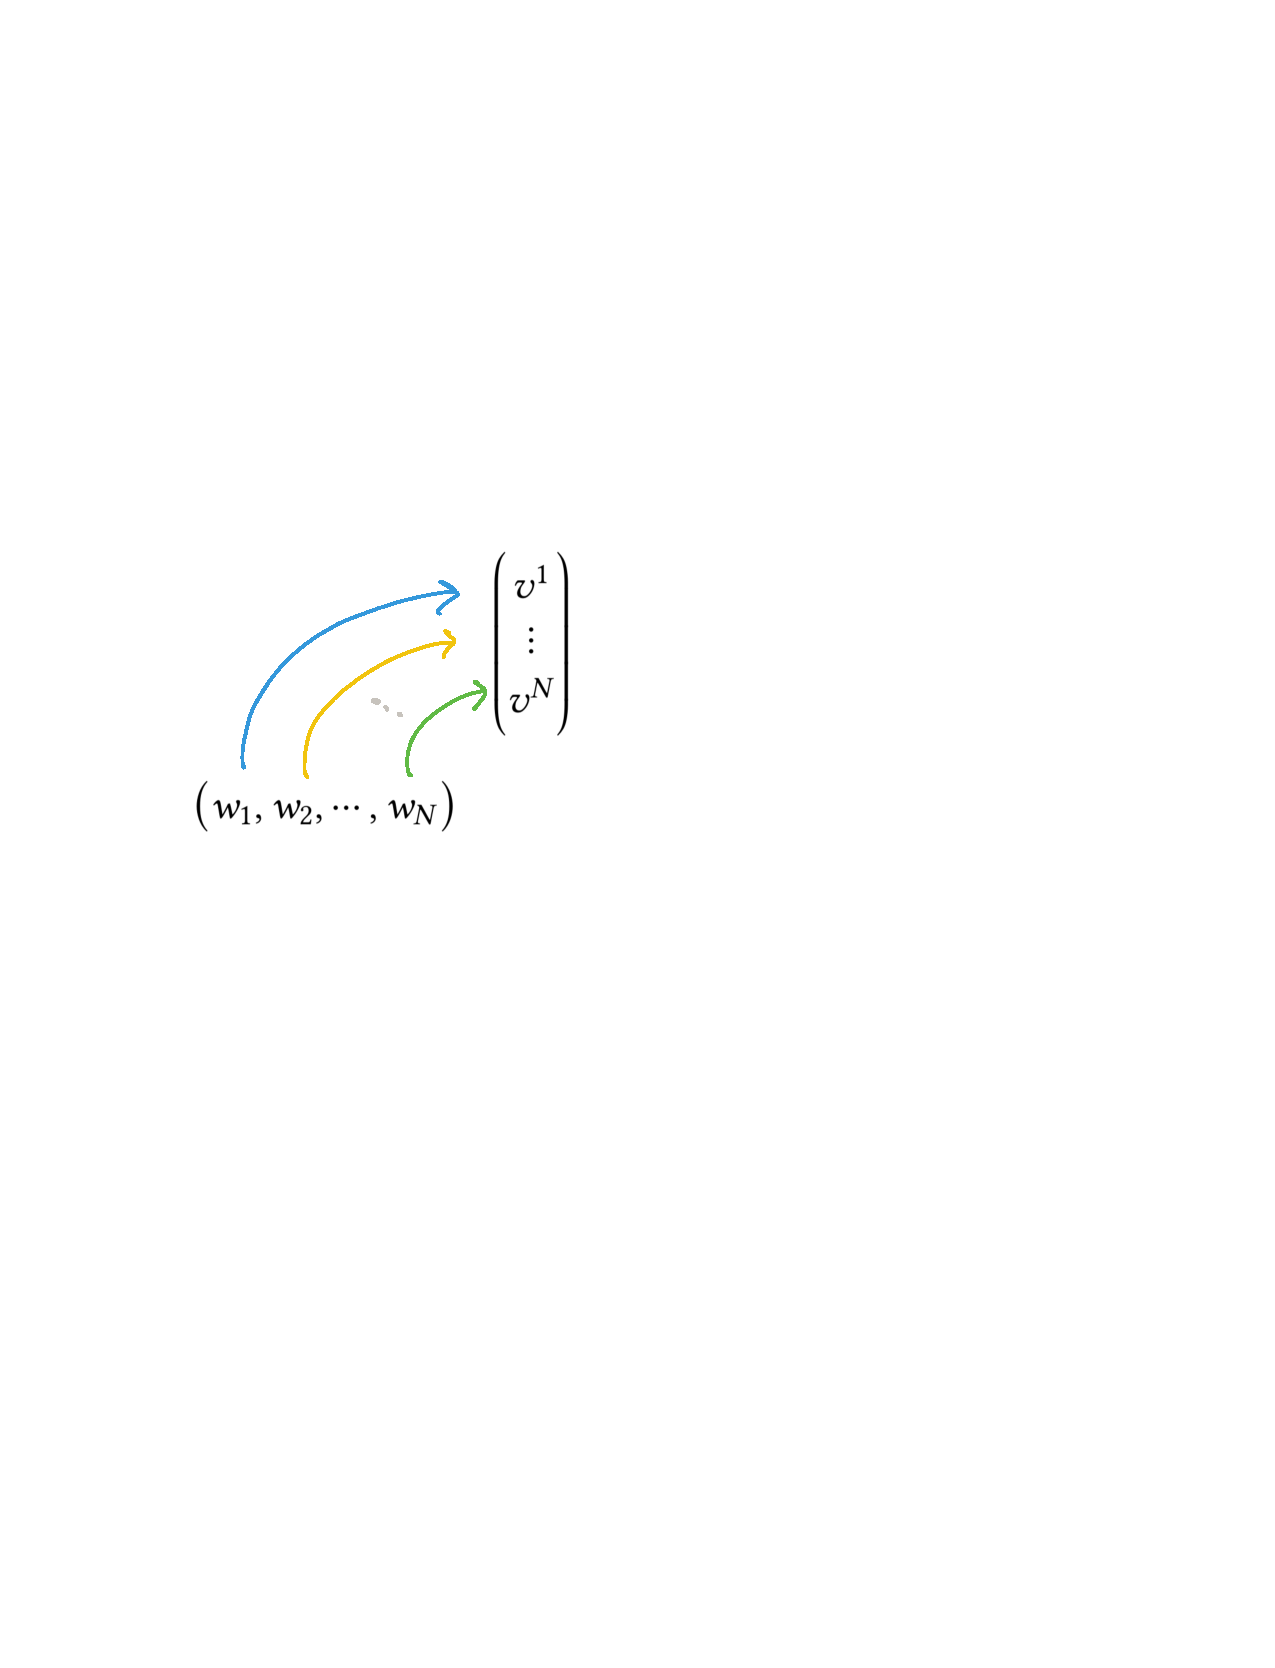
\includegraphics[width=.4\textwidth]{figures/rowcolmult.pdf}
    \caption{The `matrix multiplication rule' for acting with a row vector on a column vector.}
    \label{fig:row:col:mult}
\end{figure}
We notice that we chose to write the components of $\row{w}$ with lower indices---this is the convention. Row vectors (which have many names) have indices written as subscripts while column vectors have indices written as superscripts. There is no mathematics here, just a choice of notation. The result of the multiplication is simply a number, which we can write as a sum:
\begin{align}
    \row{w}\vec{v}
    &= \sum_{i=1}^3 w_iv^i
    \equiv w_iv^i \ .
    \label{eq:row:w:on:vec:v}
\end{align}
On the right-hand side we have \emph{defined} the summation convention: \emph{whenever there is exactly one upper index and exactly one lower index with the same letter, we should understand that there is a sum over that index over all of its allowed values.} We call pairs of repeated indices where one is upper and one is lower \textbf{contracted indices}.


The value $w_iv^i$ is simply a number. It is not a vector. It does not have any ``vectorial'' (tensorial) structure. It is not an element of the vector space $\RR ^3$. It does not transform under rotations. It is \emph{just a number}. In other words, $w_iv^i$ behaves like an object with \emph{no indices}. Contracted indices ``cancel each other out.''

This is significant because we will see that indices tell us how objects transform. Evidently, column vectors and row vectors transform differently since one has an upper index and one has a lower index. Further, when we contract the two indices, we end up with something with no indices: a number that does not transform at all. This may seem like notational overkill---trust me, it is worth building this notation now. We will use it over and over.

\begin{figure}[tb]
    \centering
    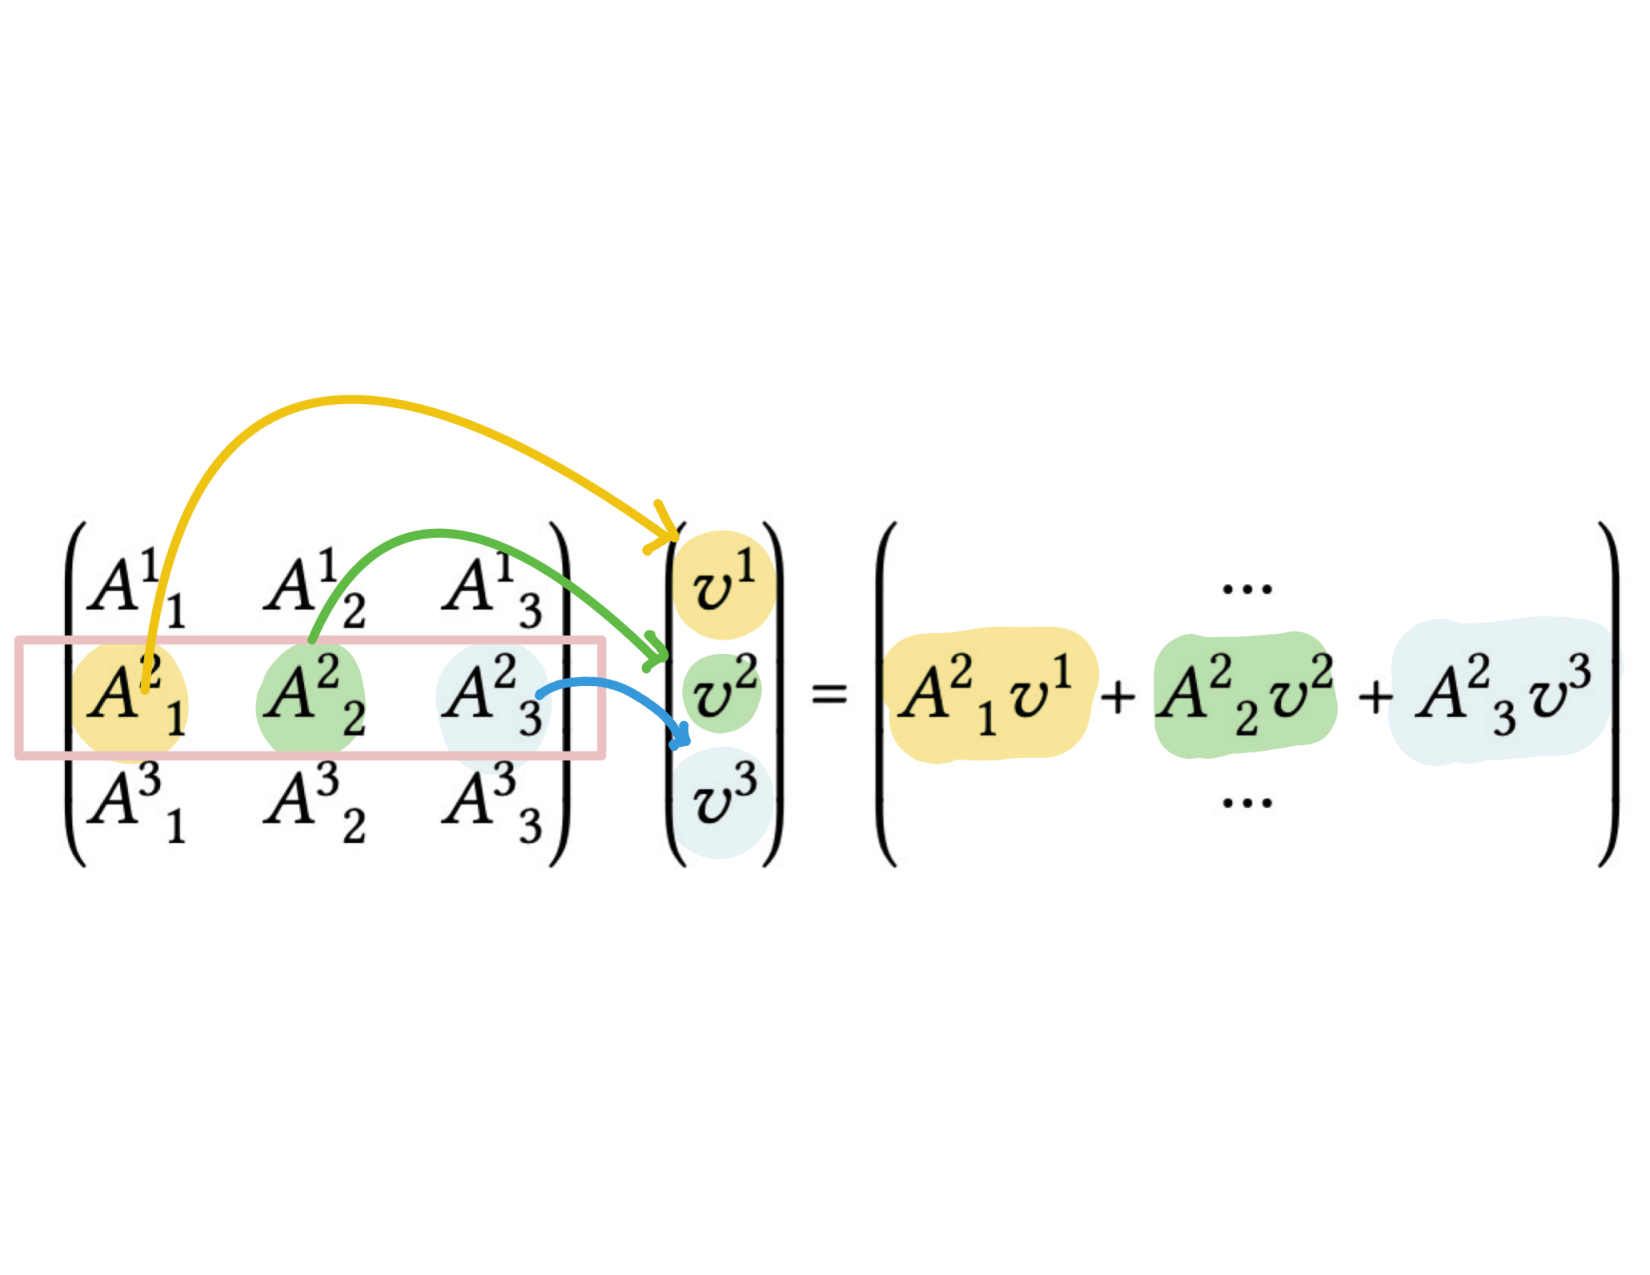
\includegraphics[width=.5\textwidth]{figures/matrixmultiplication.pdf}
    \caption{The `matrix multiplication' rule for $A\vec{v} = \vec{v}'$. We show that the second element of $\vec{v}'$ is a sum of terms, where each term is a multiplication of the $j^\text{th}$ column of the $2^\text{nd}$ row of $A$ by the $j^\text{th}$ row of $\vec{v}$.}
    \label{fig:matrix:col:mult}
\end{figure}

\begin{example}
Matrices $M$ have the following index structure: $M\aij{i}{j}$. There is a first index and a second index---the order matters. The first index is upper, and the second index is lower. Matrix multiplication boils down to a contraction of indices:
\begin{align}
    (M\vec{v})^i = M\aij{i}{j}v^j \ .
    \label{eq:matrix:mult:ith:comp}
\end{align}
Let us read this equation carefully. First, $M\vec{v}$ is a vector. The $i^\text{th}$ component of this vector is $(M\vec{v})^i$. How is this related to the components of $M$ and $\vec{v}$? The right-hand side tells us that we simply take the sum:
\begin{align}
    M\aij{i}{j}v^j = 
    M\aij{i}{1}v^1 + M\aij{i}{2}v^2  + M\aij{i}{3}v^3 \ .
\end{align}
\end{example}
\begin{example}
From the above example, you can then excuse the glib statement: ``the \emph{vector} $M\aij{i}{j}v^j$.'' As we explained above, $M\aij{i}{j}v^j$ is not a vector, but a component of a vector. However, the point is that even though there are three indices, two of them are contracted so the object effectively only has one upper index. This is the index structure of a vector. This matches the usual matrix multiplication rule shown in Fig.~\ref{fig:matrix:col:mult}.
\end{example}

\begin{exercise}
Consider the following vector, row vector, and matrix:
\begin{align}
    \vec{v} &=
    \begin{pmatrix}
     1 \\ 2 \\ 3   
    \end{pmatrix}
    &
    \row{w} &=
    \begin{pmatrix}
        4&5&6
    \end{pmatrix}
    &
    M&=
    \begin{pmatrix}
        1 & 2 & 3 \\
        4 & 5 & 6 \\
        7 & 8 & 9
    \end{pmatrix} \ .
\end{align}
These have index structure $v^i$, $w_i$, and $M\aij{i}{j}$ respectively. Note that the first index of a matrix is the row and the second is the column, thus $M\aij{1}{2} = 2$ while $M\aij{2}{1} = 4$. Calculate the following: $(wM)_2$, $(Mv)^1$, $(MM)\aij{1}{2}$. Here $MM$ is understood to be the square of the matrix $M$, $(M^2)\aij{i}{j} = M\aij{i}{k}M\aij{k}{j}$.
\end{exercise}

\begin{example}\label{eg:moving:coefficients:around}
It should be clear that
\begin{align}
    w_i M\aij{i}{j} = 
    w_1 M\aij{1}{j} + w_2 M\aij{2}{j} + w_3 M\aij{3}{j}
    = 
    M\aij{1}{j}w_1  + M\aij{2}{j}w_2 + M\aij{2}{j}w_2
    =
    M\aij{i}{j}w_i \ .
\end{align}
After all, each of the components $w_i$ and $M\aij{i}{j}$ are simply numbers. However: even though $w_i M\aij{i}{j} = M\aij{i}{j}w_i$, it is \emph{completely incorrect} to say $\row{w}M = M\row{w}$. This is because $\row{w}$ and $M$ are \emph{tensorial} (vector-y) objects. The order of their `multiplication' matters. You can see this from the matrix notation.
\begin{align}
    \row{w}M &= 
    \begin{pmatrix}
        4&5&6
    \end{pmatrix}
    \begin{pmatrix}
        1 & 2 & 3 \\
        4 & 5 & 6 \\
        7 & 8 & 9
    \end{pmatrix}
    &
    M\row{w} &=
    \begin{pmatrix}
        1 & 2 & 3 \\
        4 & 5 & 6 \\
        7 & 8 & 9
    \end{pmatrix}
    \begin{pmatrix}
        4&5&6
    \end{pmatrix} \ .
\end{align}
The first multiplication gives a row vector, as you expect since $(wM)_j$ has one lower index. The second multiplication does not even make sense. What we see is that expressions like $w_i M\aij{i}{j} = M\aij{i}{j}w_i$ are valid as long as you are only talking about the components. The glib ``physicist slang'' of replacing a component by its vector/matrix/tensor can get you into trouble if you have moved components around in a way that is only allowed for numbers, but not vectory-things.
\end{example}

Since the language is now becoming cumbersome, let us define the word \textbf{tensorial} to mean an object with indices. This will replace the phrase ``vectory'' in our notes.




One neat thing about this is that our convention for contracting indices makes it clear that $(Mv)^i$ is a component of a vector: it has one upper index. Similarly, you may recall that the multiplication of matrices $M$ and $N$ proceeds as follows:
\begin{align}
 (MN)\aij{i}{j} = M\aij{i}{k}N\aij{k}{j} \ .
 \label{eq:matrix:matrix:multiplication}    
\end{align}
\begin{exercise}
Confirm that \eqref{eq:matrix:matrix:multiplication} holds for $2\times 2$ matrices.
\end{exercise}
On the right-hand side of \eqref{eq:matrix:matrix:multiplication}, we have one pair of contracted indices ($k$), one upper index $i$, and one lower index $j$. We thus deduce that this object is a matrix: it has one upper and one lower index. Indeed, the product of two matrices is also a matrix. Our indices and contraction rules tell us what kinds of objects we can produce by contracting indices between them. 

\begin{example}
You may also contract indices within an object. For example, because a matrix has one upper and one lower index, you may contract them together. This is called the trace, $\Tr M = M\aij{i}{i}$.
\end{example}





\section{Matrices and Linear Transformations}

Vectors are the `nouns' in linear algebra. The word `linear' refers to the the \emph{verbs}. That is: we would like to act on vectors. 







\subsection{Jargon}\label{sec:jargon:linear:map}
Let us introduce some jargon here. Rather than formal definitions, we give practical ``physicist's'' definitions.\footnote{If we do something less formally, we say that we are physicists, not mathematicians. If we choose to be more highbrow, then we say that we are physicists, not engineers.} You can look up proper definitions in your favorite mathematics textbook.  The following words are closely related: function, map, transformation. I often use them interchangeably, though this is rather sloppy.  

A \textbf{function} is a mathematical machine that takes some inputs and produces some output. The inputs can be numbers, vectors, or more sophisticated objects. The outputs may also be numbers, vectors, or more sophisticated objects. The outputs do not have to be the same type of object as the inputs---in general they are not.
% 
A function that takes one input and returns one output is called a \textbf{map}. 
% 
A map that takes one type of object and returns the same type of object is called a \textbf{transformation}. Mathy-folks like to draw diagrams like Fig.~\ref{fig:Linear Transformation}.

\begin{example}
The dot product is a \textbf{function} that takes in two vectors and outputs a number.
\end{example}
\begin{example}
The magnitude is a \textbf{map} that takes a vector and returns a number.
\end{example}
\begin{example}
A function $f(x,y)=z$ is not a map because it takes two inputs.
\end{example}
\begin{example}
The national weather service website can tell you the temperature in your location as a function of the time of day. In this sense, it is a map from time to temperature.
\end{example}
\begin{example}
The map that takes a vector and returns its unit vector is a \textbf{transformation}: it is a function that takes a vector and returns a vector.
\end{example}
\begin{example}
The function that takes the a time in Pacific standard and converts it to East Coast standard is a transformation. It transforms one time (2:00pm) to another time (5:00pm).
\end{example}

\begin{figure}[tb]
    \centering
    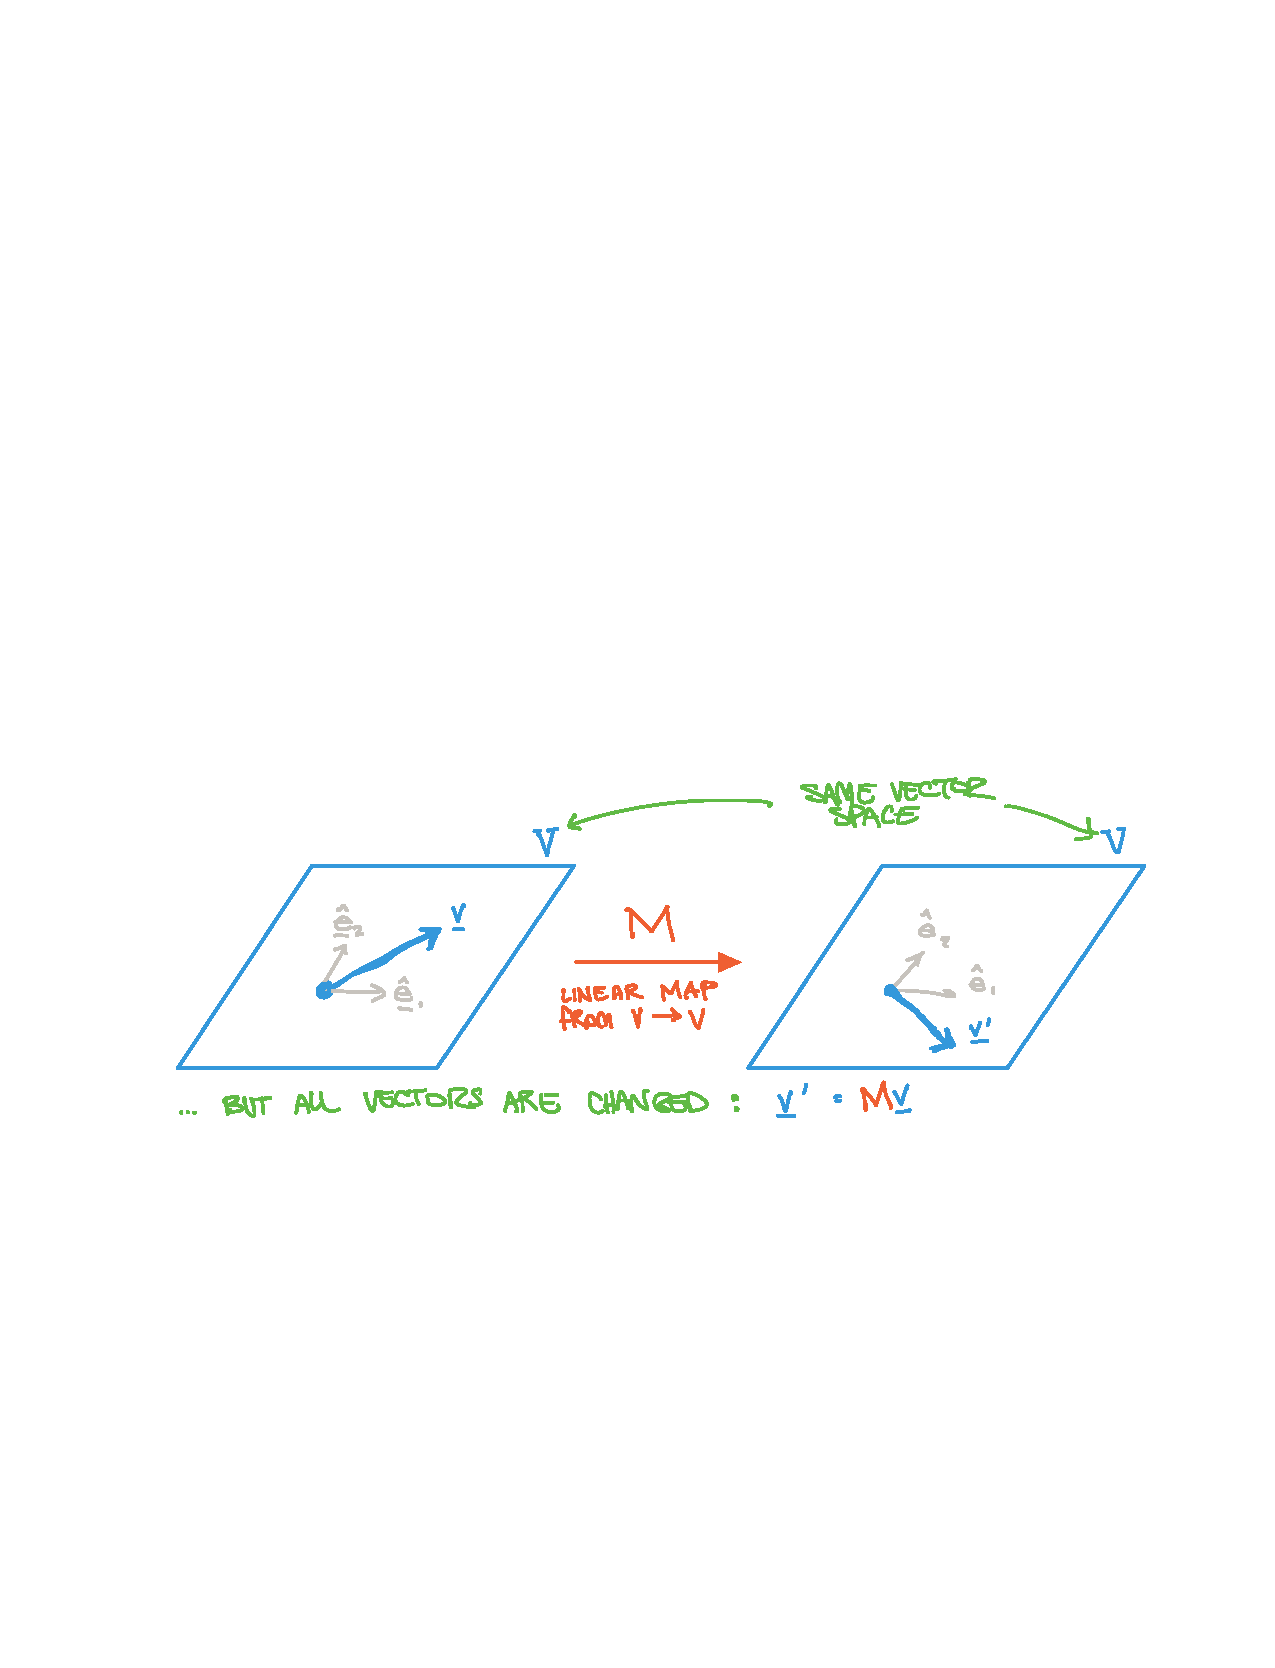
\includegraphics[width=\textwidth]{figures/lineartransformation.pdf}
    \caption{Example of a linear transformation. The transformation $M$ (for matrix) takes a vector $\vec{v}$ and turns it into a different vector that we call $\vec{v}'$. This new vector is related to $\vec{v}$ by the matrix $\vec{v'}=M\vec{v}$. \emph{Every} vector is transformed under the map $M$. This is an \emph{active transformation} where all vectors transform, but the basis (${\bas{e}}_i$) stays fixed.}
    \label{fig:Linear Transformation}
\end{figure}



\subsection{Linear transformations}


A function $f$ is \textbf{linear} if it satisfies:
\begin{align}
  f(\alpha x) &= \alpha f(x)
  &
  f(x+y) &= f(x) + f(y) \ .
  \label{eq:def:pre:linear}
\end{align}
Here $\alpha$ is a number, and $x$ and $y$ are some objects (perhaps vectors) on which the function has been defined to act. We may combine these two properties to write the condition of linearity in equation:
\begin{align}
  f(\alpha x + \beta y) = \alpha f(x)+\beta f(y)
  \label{eq:def:linear}
\end{align}
\begin{exercise}
Show that equations \eqref{eq:def:pre:linear} and \eqref{eq:def:linear} imply one another. Going from \eqref{eq:def:pre:linear} to \eqref{eq:def:linear} is slightly more tricky than the other way around.
\end{exercise}


\subsection{Linear Transformations in One Dimension}

The definition of `linear' has \emph{nothing to do with lines}. It is true that $y=mx+b$ is the equation for a line in the $(x,y)$ plane. This is not the same as $f(x)=mx+b$ being linear. In fact, $f(x)=mx+b$ is \emph{not} linear as a transformation of numbers, $\RR \to\RR $
\begin{exercise}
Show that $f(x) = mx+b$ does \emph{not} satisfy the definition of linearity, \eqref{eq:def:linear}. It is sufficient, for example, to consider $f(2x) \stackrel{?}{=}f(x)+f(x)$. Another cute way to see this is to consider linear combinations with zero, say $f(x+0)$.
\end{exercise}

\begin{exercise}
Show that $f(x) = mx$ is linear.
\end{exercise}

The problem in $f(x)=mx+b$ is the shift by a constant, $b$. I will comment that we can make up mathematics where `shift by a constant' is allowed. This, however, is no longer \emph{linear algebra}. You can look up affine spaces\footnote{\url{https://en.wikipedia.org/wiki/Affine_space}} if are curious. I only mention it here because the word `affine' may show up later in your mathematical physics studies---I want you to remember that it has something to do with constant shifts. 

\subsection{Linear Transformations in Two and Three Dimensions}

In Section~\ref{sec:index:notation} we introduced the idea that a matrix, $M$ has a peculiar index notation $M\aij{i}{j}$. This turned out to be convenient because we could use Einstein summation convention to conveniently write out what happens when we apply a matrix $M$ to a vector $\vec{v}$. You end up with a vector $M\vec{v}$ with components
\begin{align}
    (Mv)^i = M\aij{i}{j}v^j \ .
\end{align}
We recognized that the $j$ indices are \emph{contracted}. From an index point of view, these contracted indices ``cancel out'' so the resulting expression  only has one free index.\footnote{I say \emph{free} index to contrast it from a contracted (repeated) index that is summed over. We can put any allowed value into a free index and the equation is true.} This is good, the left-hand side of the above equation has one free index, so the right-hand side should also have exactly one free index.\footnote{This should remind you of dimensional analysis. If you have different dimensions on two sides of an equation, you have done something wrong.}




\subsection{The trivial transformation: identity matrix}

The identity matrix, $\one $ leaves vectors unchanged: $\one \vec{v} = \vec{v}$. You already know its components in $\RR ^3$:
\begin{align}
    \one  = 
    \begin{pmatrix}
        1 & 0 & 0 \\
        0 & 1 & 0 \\
        0 & 0 & 1
    \end{pmatrix} \ .
\end{align}
Sometimes we will indicate the dimension of the space by writing $\one _3$ or $\one _{3\times 3}$ when we want to be extra clear. There is a useful way of writing the components of the identity matrix. Define the \textbf{Kronecker}~$\delta$: 
\begin{align}
    \delta^i_j &= 
    \begin{cases}
    1 & \text{ if }\, i=j\\
    0 & \text{ if }\, i\neq j
    \end{cases} \ .
\end{align}
Then we say that the components of $\one $ are $\delta^i_j$, no matter what dimension of space we are in.

\emph{But wait}, you object, \emph{the indices are all messed up!} You are right. The indices on $\delta^{i}_j$ look wrong because we made a big deal that matrices have a first index and a second index that we must distinguish between. The first index is written upper, and the second index is lower. So should we not have written $\delta\aij{i}{j}$, with the $j$ clearly to the right of the $i$? 

Yes, this is technically correct. The reason why we made a big deal about this and wrote $M\aij{i}{j}$ instead of $M^i_j$ is that we will eventually want to consider alternative configurations of indices. For example, $T_{ij}$ or $S_i^{\phantom{i}j}$ or even weirder things like $R^\mu_{\phantom{\mu}\nu\rho\sigma}$.  It turns out that for the identity matrix, there is no ambiguity because
\begin{align}
    \delta^i_j = \delta\aij{i}{j} = \delta_i^{\phantom{i}j} .
\end{align}
So for convenience, we will just write $\delta^i_j$. Observe, however, that we \emph{never} write $\delta_{ij}$. There is no problem defining $\delta_{ij}$ in the same way, but it turns out that this combination rarely shows up.\footnote{Instead, there is a different mathematical structure called the metric, $g_{ij}$ that has two lower indices. Sometimes the metric components may be equal to the Kronecker $\delta$, so we may say $g_{ij}$ = $\delta_{ij}$. But in those cases we need to be clear that we are using the metric that happens to be the identity, not that we are multiplying by the identity. Why the big deal? One example is that the metric is where gravity lives---so it would be a rather big omission if we mistook it for ``multiplying by one.''}

It is useful to think about the Kronecker~$\delta$ as a machine that converts indices. Consider what it does to a vector:
\begin{align}
    (\one \vec{v})^i = \delta^i_j v^j = 
    \delta^i_1v^1 + \delta^i_2v^2 + \delta^i_3v^3 \ .
\end{align}
On the right-hand side, there is exactly one non-zero term because $\delta^i_j$ is zero for all terms except when $j=i$. That means 
\begin{align}
    \delta^i_j v^j = v^i \ .
    \label{eq:kronecker:delta:action}
\end{align}
The right-hand side is, of course, what we expected since $\one \vec{v} = \vec{v}$. So we can train ourselves to ``mechanically'' interpret the $\delta^i_j$ object as one that replaces indices. 
\begin{exercise}
Show that this works for lower indices as well. Consider the multiplication of two matrices, $M\one $. Show that
\begin{align}
    M\aij{i}{j}\delta^j_k = M\aij{i}{k} \ ,
\end{align}
so that the $\delta^j_k$ simply replaces the $j$ index on $M\aij{i}{j}$ and turns it into a $k$.
\end{exercise}
\begin{exercise}
Even though we have not introduced any objects with more complicated index structure, suppose you have the following object: 
\begin{align}
    R^\mu_{\phantom{\mu}\nu\rho\sigma} \ .
\end{align}
The Greek letters are indices (like $i$ and $j$), we have switched notation because this is the convention for spacetime. An object with this index structure shows up in general relativity, it is called the Riemann tensor. Without knowing any general relativity, write out the value of
\begin{align}
    \delta^\mu_\alpha\,
    \delta^\nu_\beta\,
    \delta^\rho_\gamma\,
    \delta^\sigma_\tau\,
    R^\mu_{\phantom{\mu}\nu\rho\sigma} \ .
\end{align}
This is some kind of `matrix multiplication' by `identity matrices' hitting a $N\times N\times N\times N$ array of numbers, where $N=4$ is the dimension of spacetime. 
\end{exercise}

\subsection{Composition of linear transformations}

Suppose you have two linear transformations from $V\to V$, call them $f(\vec{x})$ and $g(x)$. These are represented by matrices $M$ and $N$, repectively. Then the \textbf{composition} of these two linear transformations is
\begin{align}
    f\circ g(\vec{x}) &\equiv f\left(g(\vec{x})\right)
    &
    \Leftrightarrow
    &
    f\circ g(\vec{x})&=
    MN\vec{x}
\end{align}
On the right-hand side we have written the matrix that represents $f\circ g$ as the product of the matrices for $f$ and $g$: $MN$. Matrix multiplication follows the usual rules. We can write this using summation convention very nicely. The matrices have components and index structure $M\aij{i}{j}$ and $N\aij{i}{j}$ respectively. Each has an upper index and a lower index. The product $MN$ has components
\begin{align}
    (MN)\aij{i}{j} = M\aij{i}{k}N\aij{k}{j} \ .
    \label{eq:matrix:multiplication}
\end{align}

\begin{example}
One thing that we notice from \eqref{eq:matrix:multiplication} is that the index structure makes it clear that the order of matrix multiplication matters.
\begin{align}
    (MN)\aij{i}{j} = M\aij{i}{k}N\aij{k}{j} 
    \neq 
    N\aij{i}{k}M\aij{k}{j} 
    =
    (NM)\aij{i}{j} \ .
\end{align}
Thus the order in which two linear transformations are composed matters. On the other hand, the order in which components (which are just numbers) are multiplied does not matter. For example:
\begin{align}
    (MN)\aij{i}{j} 
    = M\aij{i}{k} N\aij{k}{j}  
    = N\aij{k}{j} M\aij{i}{k} \ .
\end{align}
The sums on the right-hand side both represent the same series of terms. Neither of those sums are the same as 
\begin{align}
    (NM)\aij{i}{j}
    =
    N\aij{i}{k}M\aij{k}{j}
    =
    M\aij{k}{j} N\aij{i}{k} \ .
\end{align}
This is the kind of manipulation that is pretty obvious at its core, but the first time you see this manipulation done in textbook it can be pretty disorienting. 
\end{example}
The above example makes the following point clear: The order in which components are multiplied is \emph{not} the same as the order in which the linear transformations are applied. That is, the order of the components are multiplied not the same as the order in which the matrices are multiplied.
\begin{example}
If you want to recover the ``matrix multiplication'' $MN$ from the ``component contraction'' $M\aij{i}{k} N\aij{k}{j}  
    = N\aij{k}{j} M\aij{i}{k}$, you should start by writing out the terms so that neighboring indices are contracted. The expression $M\aij{i}{k} N\aij{k}{j}$ has neighboring $k$ indices contracted, while the equivalent expression $N\aij{k}{j} M\aij{i}{k}$ does not. Thus we take $M\aij{i}{k} N\aij{k}{j}$ and then we can ``promote'' this back to a matrix multiplication, $MN$. A caveat: physicists often prefer to work with component contractions instead of matrix multiplications. In fact, with more complicated tensor contractions, it is not always meaningful or possible to recover a ``matrix multiplication'' form.
\end{example}


\begin{exercise}\label{ex:product:of:diagonal:matrices}
A \textbf{diagonal matrix} is one where the only non-zero components are along the diagonal. We will sometimes write diagonal matrices with a hat, $\hat M$, to indicate that they are diagonal. Sometimes we abbreviate the definition of a diagonal matrix by only specifying its diagonal components:
\begin{align}
    \hat M = 
    \begin{pmatrix}
        2 & 0 & 0 \\
        0 & 7 & 0 \\
        0 & 0 & 4  
    \end{pmatrix}
    =
    \text{diag}(2,7,4) \ .
\end{align}
Show that the product of diagonal matrices is also diagonal whose components are the products of the diagonal components. You can use \eqref{eq:matrix:multiplication} armed with the knowledge that $(\hat M)\aij{i}{j} = 0$ if $i\neq j$. Then you must show that $(\hat M \hat N)\aij{i}{j} = 0$ for $i\neq j$. Finally, check the values of the diagonal elements to show that
\begin{align}
    \hat M \hat N = \text{diag}\left(M\aij11 N\aij11 \;,\;\, M\aij22 N\aij 22 \;,\;\, M\aij33 N\aij 33\right) \ .
\end{align}

\end{exercise}


\subsection{Linearity and Basis Vectors}

\paragraph{A couple of useful exercises}
Here's a pair of exercises that are worth trying out:
\begin{exercise}
Calculate the following linear transformations by a matrix $M$ on two different vectors, $\vec{v}$ and $\vec{w}$:
\begin{align}
    M\vec{v} &= 
    \begin{pmatrix}
        \pp 3 & 2 & \pp 1 \\
        - 1 & 4 & -2 \\
        \pp 0 & 1 & \pp 1
    \end{pmatrix}
    \begin{pmatrix}
        2 \\ 1 \\ 1
    \end{pmatrix}
    = \quad ?
    &
    M\vec{w} &= 
    \begin{pmatrix}
        \pp 3 & 2 & \pp 1 \\
        - 1 & 4 & -2 \\
        \pp 0 & 1 & \pp 1
    \end{pmatrix}
    \begin{pmatrix}
        -1 \\ \pp 0 \\ 3
    \end{pmatrix}
    = \quad ?
\end{align}
\end{exercise}
\begin{exercise}
That was tedious, wasn't it? What if I asked you to calculate three more...
\begin{align}
    M
    \begin{pmatrix}
        1 \\ 1 \\ 4
    \end{pmatrix}
    &= \quad ?
    &
    M
    \begin{pmatrix}
        0 \\ 1 \\ 7
    \end{pmatrix}
    &= \quad ?
    &
    M
    \begin{pmatrix}
        \pp 3 \\ \pp 1 \\ -2
    \end{pmatrix}
    &= \quad ?
    \label{eq:eg:more:multiplications}
\end{align}
\end{exercise}
Did you do it? Go ahead, do these calculations. Use \emph{Mathematica} if you must. Did you do it the hard way, or did you notice that there's an easy way? 

\paragraph{General two-dimensional discussion}
The easy observation is that each of the vectors being acted on in \eqref{eq:eg:more:multiplications} are \textbf{linear combinations} of $\vec{v}$ and $\vec{w}$. What you should notice is that
\begin{align}
    \begin{pmatrix}
        1 \\ 1 \\ 4
    \end{pmatrix}
    = \vec{v} + \vec{w}
    &
    & 
    M
    \begin{pmatrix}
        1 \\ 1 \\ 4
    \end{pmatrix}
    &=
    M(\vec{v} + \vec{w})
    = M\vec{v} + M\vec{w} \ .
\end{align}
In other words: if $\vec{u} = \vec{v} + \vec{w}$ and we already know the action of a matrix $M$ on $\vec{v}$ and $\vec{w}$---that is, we know $M\vec{v}$ and $M\vec{w}$---then we're basically done. No further matrix multiplication is needed! We can simply use the linearity of $M$ to take a linear combination of $M\vec{v}$ and $M\vec{w}$. You should check that this is true for the other matrix multiplications in \eqref{eq:eg:more:multiplications}.


This is a big deal. We know that $\vec{v}$ and $\vec{w}$ are the \textbf{basis vectors} for a subspace $V_2 = \text{Span}(\vec{v},\vec{w})$. We have established that if we know the action of $M$ on the basis vectors of $V_2$, then we know the action of $M$ on any vector in $V_2$. This is because any vector in $V_2$ has the form
\begin{align}
    \vec{u} = a\vec{v} + b \vec{w}
\end{align}
for two numbers $a$ and $b$. Then the action of $M$ on any such vector is
\begin{align}
    M\vec{u} = a(M\vec{v}) + b(M\vec{w}) \ .
    \label{eq:Mu:aMv:bMw}
\end{align}

We can pose this in the following way. Suppose we have a two-dimensional vector space $V_2$
 with some basis $\vec{b}_1$ and $\vec{b}_2$. Now suppose we have a linear transformation $M$ that goes from $V_2\to V_2$. This is a matrix. 
\begin{enumerate}
    \item We know that the matrix is encoded by $2\times 2= 4$ numbers, each of the four elements, $M\aij{i}{j}$. If you know these four elements, then you can matrix multiply any vector in $V_2$ by simply using the matrix multiplication rules. All you need to specify is the vector $\vec{u}$, which is encoded by its two components $u^i$. Then you get two numbers as output, $(Mu)^i = M\aij{i}{j}u^j$.
    \item Alternatively, we suppose that we do not know (or we deliberately forget) the four elements $M\aij{i}{j}$. Instead, suppose we know the components of $M\vec{v}$ and $M\vec{w}$. These are each two component vectors, so this is a total of four numbers. Then we may specify $\vec{u}$ not by its components $u^i$, by its coefficients $a$ and $b$. Then we may use \eqref{eq:Mu:aMv:bMw} to specify the two components of $M\vec{u}$.
\end{enumerate}
In each picture, you specify the four numbers that encode the transformation and then use them to calculate the action of $M$ on a generic vector $\vec{u}$. 

\begin{example}
The two approaches above are equivalent when the basis vectors are
\begin{align}
    \vec{b}_1 = {\bas{e}}_1 &= \begin{pmatrix}
        1 \\ 0
    \end{pmatrix}
    &
    \vec{b}_2 = {\bas{e}}_2 &= \begin{pmatrix}
        0 \\ 1
    \end{pmatrix}\ .
\end{align}
This should be clear since
\begin{align}
    M {\bas{e}}_1 &= 
    \begin{pmatrix}
        M\aij{1}{1} \\ M\aij{2}{1}
    \end{pmatrix}
    &
    M {\bas{e}}_2 &= 
    \begin{pmatrix}
        M\aij{1}{2} \\ M\aij{2}{2}
    \end{pmatrix} \ .
    \label{vec:Mhate:2}
\end{align}
\end{example}
The example above tells us that the `components of a matrix' have a specific meaning: they encode the action of $M$ on a particularly nice basis, ${\bas{e}}_{1,2}$. This is significant for the following reason: while a matrix may encode a linear transformation, we should not be settle into thinking that the $2\times 2$ of numbers somehow \emph{is} the matrix.
\begin{example}
$M\aij 11$ is simply the coefficient of ${\bas{e}}_1$ in the expansion of $M{\bas{e}}_1$. $M\aij 12$ is simply the coefficient of ${\bas{e}}_2$ in the expansion of $M{\bas{e}}_1$. 
\end{example}
Another way of saying this is the following:
\begin{bigidea}
The $i^\text{th}$ column of a matrix are the components of $M\bas{e}_i$. This assumes that $\bas{e}_i$ is ``canonical'' basis which has the $i^\text{th}$ element set to one and the rest of the elements are zero.
\end{bigidea}



 

\paragraph{General discussion}
The general version of this discussion is as follows. We write $\RR ^N$ to be $N$-dimensional real space. A linear transformation from $\RR ^N \to \RR ^N$ is a matrix. Suppose we have a nice basis. In fact, the `obvious' basis is
\begin{align}
    {\bas{e}}_1 &= 
    \begin{pmatrix}
        1 \\ 0 \\ 0 \\ \vdots
    \end{pmatrix}
    &
    {\bas{e}}_2 &= 
    \begin{pmatrix}
        0 \\ 1 \\ 0 \\ \vdots
    \end{pmatrix}
    &
    \cdots &
    &
    {\bas{e}}_N &= 
    \begin{pmatrix}
        0 \\ \vdots \\ 0 \\ 1
    \end{pmatrix} \ .
\end{align}
Then we know that any vector in $\RR ^N$ may be written as a linear combination of these basis vectors. In fact, this is \emph{precisely} what we mean by the components of a vector: it is the coefficient of each ${\bas{e}}_i$ basis vector in the linear combination that represents the vector:
\begin{align}
    \vec{v} &= v^i{\bas{e}}_i 
    &
    \vec{v} &\;\text{``=''}\;
         \begin{pmatrix}
        v^1 \\ v^2 \\ \vdots \\ v^N
    \end{pmatrix} \ .
\end{align}
The first equality is \emph{true}. It defines the meaning of $v^i$ no matter what the ${\bas{e}}_i$ are, whether they are columns or more abstract objects. The equation on the right has air quotes because it is not really an equation. What it means is $\vec{v}$ \emph{is represented by the following column of numbers}. The column of numbers simply mean the coefficients of the basis vectors---no matter what the basis vectors are.


In physics, we treat lots of different things as vectors. Momenta, electric fields, wavefunctions, and so forth. When we say that the electric field at a point is a vector, we do not mean that there is actually an invisible arrow with some length and direction there. Nor do we mean that the electric field at that point is a column of three numbers. What we mean is that these three numbers represent the components of the electric field with respect to a basis. The basis are usually the electric field in the $x$, $y$, and $z$ directions. 


If we know the action of $M$ on the basis vectors, what that really means is that we know the components of $M{\bas{e}}_i$ for each $i$. That is to say, 
\begin{align}
    M{\bas{e}}_i &= (M{\bas{e}}_i)^k {\bas{e}}_k 
    &
    M\aij{k}{i} &\equiv (M{\bas{e}}_i)^k
    \ .
\end{align}
Be very careful with this. What we mean is the $N$-dimensional generalization of \eqref{vec:Mhate:2}, so refer back to that if the notation is cumbersome. What is important here is that we now have a definition of the components $M\aij{i}{j}$ that is fully general. 



\subsection{Linear transformations as maps acting on basis vectors}

The relation between the components of linear transformations and basis vectors is elucidated in Fig.~\ref{fig:map:M}. A vector is a linear combination of the basis vectors, so the action of a linear transformation $M$ on a vector $\vec{v}$ reduces to taking linear combinations of the action of $M$ on the basis vectors $\bas{e}_i$:
\begin{align}
    \vec{v} &= v^i\bas{e}_i 
    M\vec{v} &= v^i\, M\bas{e}_i 
    \ .
    \label{eq:v:Mv:basis:action}
\end{align}
There are several observations:
\begin{itemize}
    \item We could define a basis $\vec{f}_i \equiv M\bas{e}_i$. Then the components of $\vec{v}$ in the $\bas{e}_i$ basis are the same as the components of $M\vec{v}$ in the $\vec{f}_i$ basis. 
    \item The components of $M\vec{v}$ in the $\bas{e}_i$ basis are \emph{not} the $v^i$, but rather the linear combinations $M\aij{i}{j}v^j$. We know this from our matrix multiplication rules, but we can also see it from the linear combination $v^i\, M\bas{e}_i$ and the observation that the matrix components $M\aij{i}{j}$ are simply the components of $M\bas{e}_i$, as we saw in \eqref{vec:Mhate:2}.
    \item What is nice about \eqref{eq:v:Mv:basis:action} is that we have separated the \emph{components} of a vector $v^i$ from the ``vector-y'' part, $M\bas{e}_i$. What we mean by this is that the \emph{components} are just numbers. They are coefficients of a linear combination and are what we write as the components of a column of numbers. However, vectors are not always ``columns of numbers.'' We want to abstract what a vector is and thus we need to also abstract what a linear transformation is. All of that abstraction is encoded in the basis vectors and the definition of the transformation acting on the basis vectors. 
\end{itemize}


\begin{figure}[tb]
    \centering
    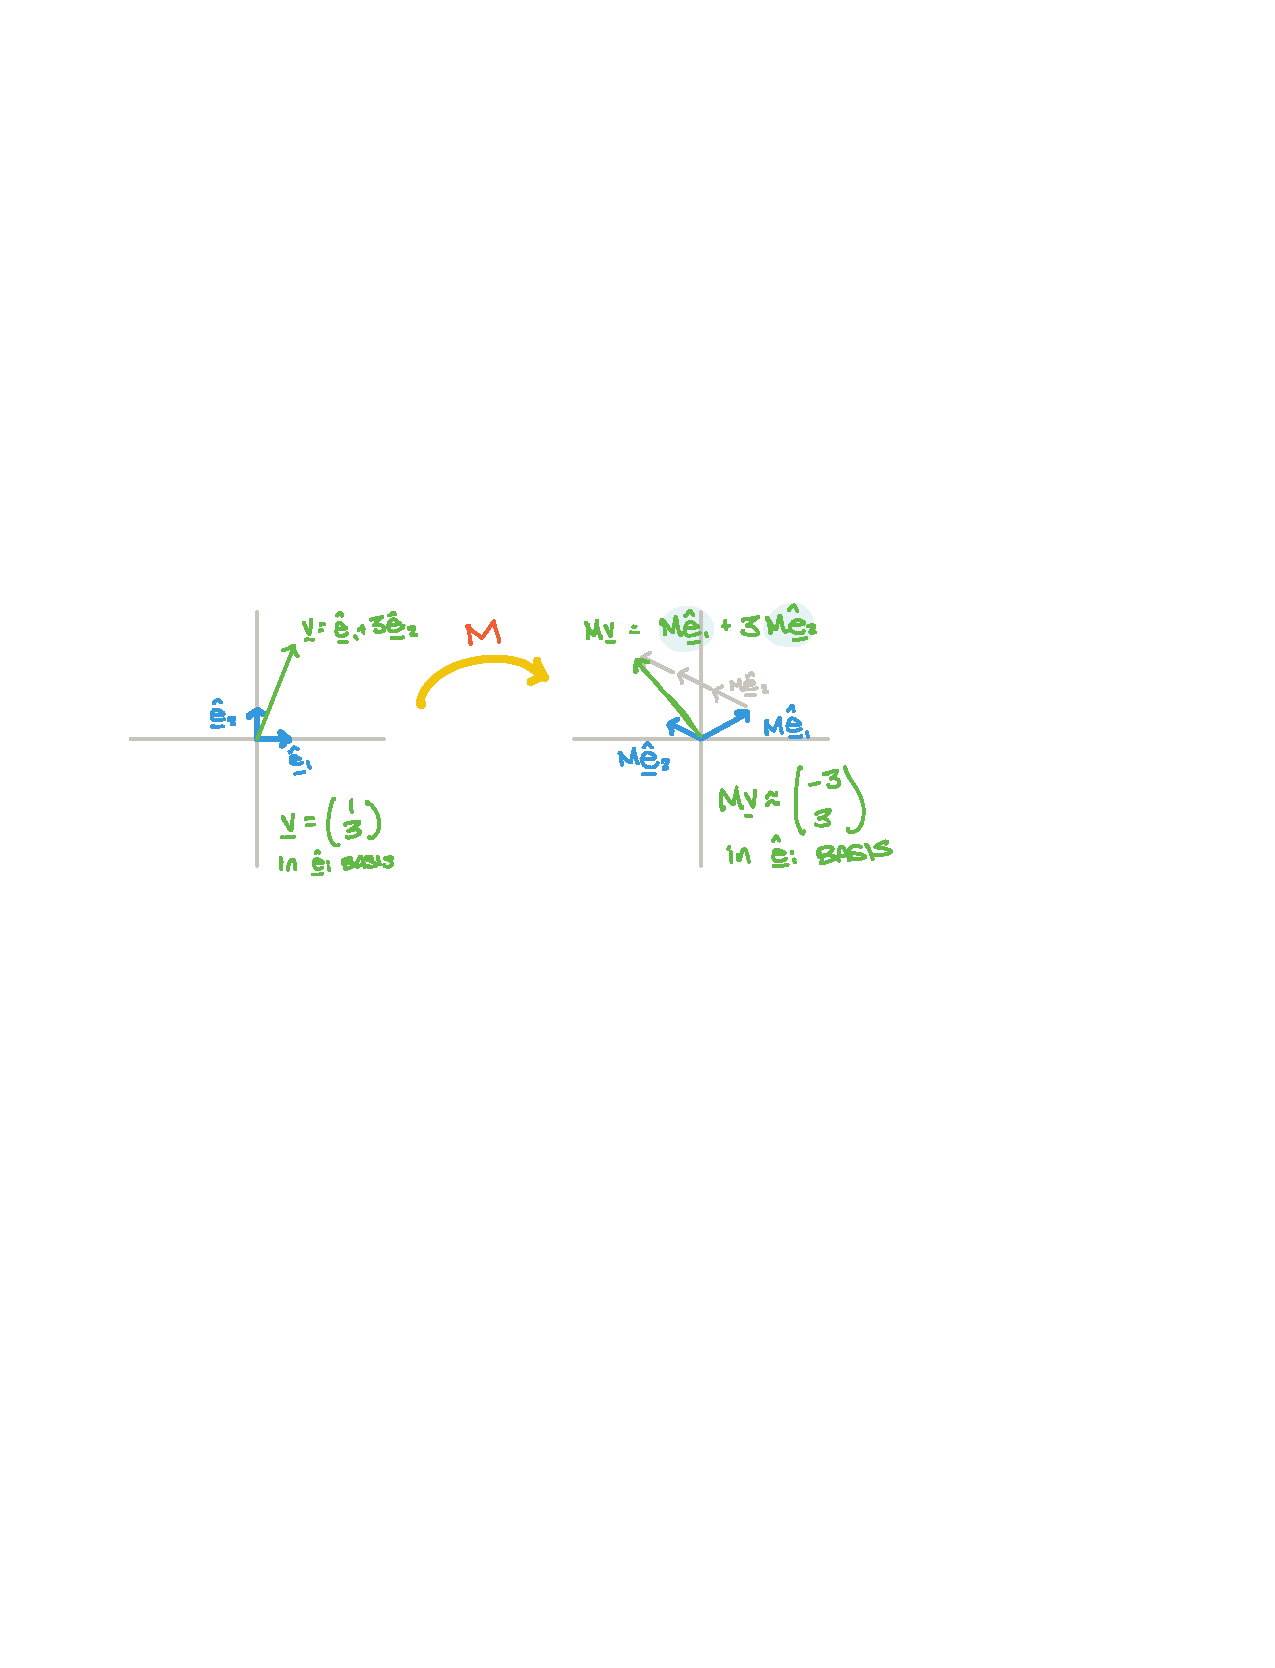
\includegraphics[width=.8\textwidth]{figures/maps_M.pdf}
    \caption{$M$ is a linear transformation from $\RR ^2\to\RR ^2$. If we know the action of $M$ on the basis vectors $\bas{e}_i$ of $\RR ^2$, then we know the action of $M$ on any vector $\vec{v}$.}
    \label{fig:map:M}
\end{figure}




\subsection{Inverse transformations}

% Pre-image, image, kernel, 
% Non-invertible

Let $M$ be a linear transformation from $V\to V$. This is just to say that $M$ is a matrix that acts on vectors in $V$. For ``nice'' matrices, $M$, there is a unique \textbf{inverse} matrix (inverse transformation) $M\inv$ with components $(M\inv)\aij{i}{j}$. The defining property of the matrix inverse is $M\inv M = \one $. That means that $M\inv(M\vec{v})=\vec{v}$ for any vector $\vec{v}$. The matrix inverse simply undoes the transformation $M$. This is shown in Fig.~\ref{fig:map:M:inv}. 

% \flip{in progress}
% not always defined.


\begin{figure}[tb]
    \centering
    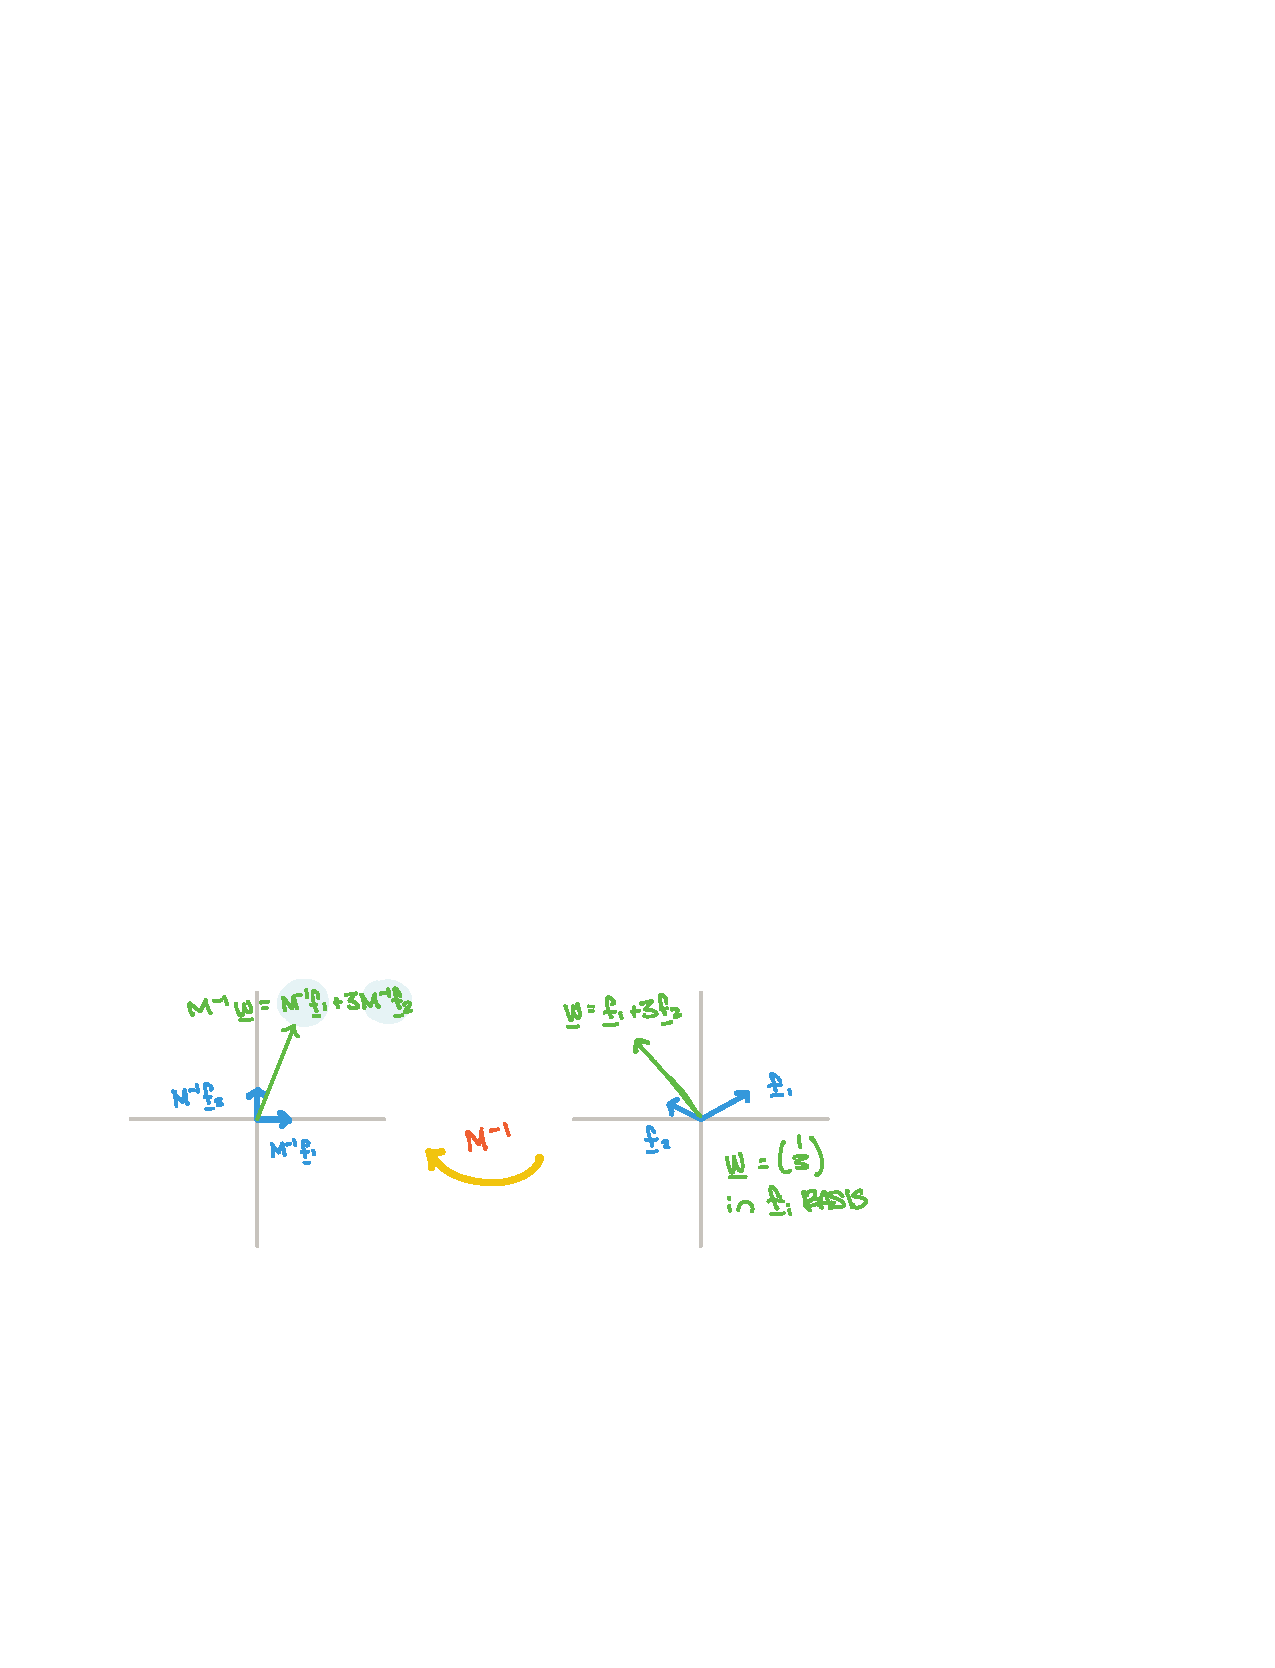
\includegraphics[width=.8\textwidth]{figures/maps_Minv.pdf}
    \caption{Let $M$ is a linear transformation from $\RR ^2 \to \RR ^2$, as we drew in Fig.~\ref{fig:map:M}. Now assume that you have a vector $\vec{w}$ that is the linear combination of some basis vectors $\vec{f}_i$, see the right-hand side of the sketch. If the $\vec{f}_i$ can be obtained as the transformation by $M$ of some other vectors---the basis vectors we called $\bas{e}_i$ in Fig.~\ref{fig:map:M}---then the inverse transformation $M\inv$ acts as a map ``back'' to the original basis. }
    \label{fig:map:M:inv}
\end{figure}

Given a basis, matrices are described by their components, $M\aij{i}{j}$. How do you find the components of the inverse matrix, $(M\inv)\aij{i}{j}$? The most straightforward way is the hard way. Let us consider the $2\times 2$ case. We know that the defining relationship is
\begin{align}
    M(M\inv)=(M\inv)M &= \one 
    &
    M\aij{i}{k}(M\inv)\aij{k}{j}
    =
    (M\inv)\aij{i}{k}M\aij{k}{j} 
    = \delta^i_j \ .
    \label{eq:inverse:matrix:definition}
\end{align}
On the right we have four equations for each combination of $i,j \in\{1,2\}$. We also have four unknown components, $(M\inv)\aij{i}{j}$. This is a system of linear equations that one can usually solve. Sometimes the system will not be solvable---in that case the matrix $M$ is not invertible.

\begin{exercise}
Convince yourself that \eqref{eq:inverse:matrix:definition} holds for \emph{any} vector space of any dimension, $N$. You end up with $N^2$ equations for $N^2$ unknown components $M\aij{i}{j}$. Does this change if all of the components are allowed to be complex numbers?
\end{exercise}


The product of two matrices $M$ and $N$ is a matrix, $MN$. The inverse of the product of matrices is the product of their inverses \emph{in the reverse order}
\begin{align}
    (MN)\inv = N\inv M\inv \ .
\end{align}
You can that this is because you have to undo the transformation that was last applied:
\begin{align}
    (MN)\inv MN = N\inv M\inv MN = N\inv \one  N = \one  \ .
\end{align}




\begin{example}
The inverse of a diagonal matrix is easy:
\begin{align}
    M &=
    \begin{pmatrix}
     3 & \pp  0 \\
     0 & -2
    \end{pmatrix}
    &
    M\inv &=
    \begin{pmatrix}
    \frac{1}{3} & \pp 0 \\
    0 & -\frac{1}{2}
    \end{pmatrix} \ .
\end{align}
We have used the earlier observation in Exercise~\ref{ex:product:of:diagonal:matrices} that the product of diagonal matrices $\hat M$ and $\hat N$ is also a diagonal matrix whose elements are the products of the corresponding elements in $\hat M$ and $\hat N$.
\end{example}

Physical states are often described by vectors. The dynamics of a theory of physics are then described by linear transformations of vectors. Usually this is some description of the change in the vector over some infinitesimal time. This change is a response to some source of the dynamics. You end up with formulas that always look like
\begin{align}
    M \vec{v} &= \vec{s} 
    &
    \Leftrightarrow
    &
    (\text{dynamics})(\text{state}) = (\text{source}) \ .
\end{align}
The source is something like a pebble falling into a pond. The dynamics are a matrix that describes how ripples propagate. The state is the configuration of the water in the pond.
%
The problem that you have to solve in physics is usually framed as follows: If you are given some source $\vec{s}$, what is the value of the state $\vec{v}$? This requires taking the inverse of the dynamics $M$. 

Thus far we have seen two things: first, finding the components of an inverse matrix is generally very annoying. Secondly, there is at least one case---when the matrix is diagonal---where the annoying task is significantly simplified. It turns out that there are more clever ways to invert a matrix that often apply for the types of matrices that show up in physics. These tricks boil down to converting matrices into their diagonal form.



\subsection{Matrices that aren't invertible: Projections}

Solving for the components of a matrix inverse boils down to $N^2$ equations for $N^2$ unknowns. This does not mean that those equations have a solution. A simple example is the case of a diagonal matrix with one component zero. We illustrate this in Fig.~\ref{fig:map:M:no:inv}
\begin{figure}[tb]
    \centering
    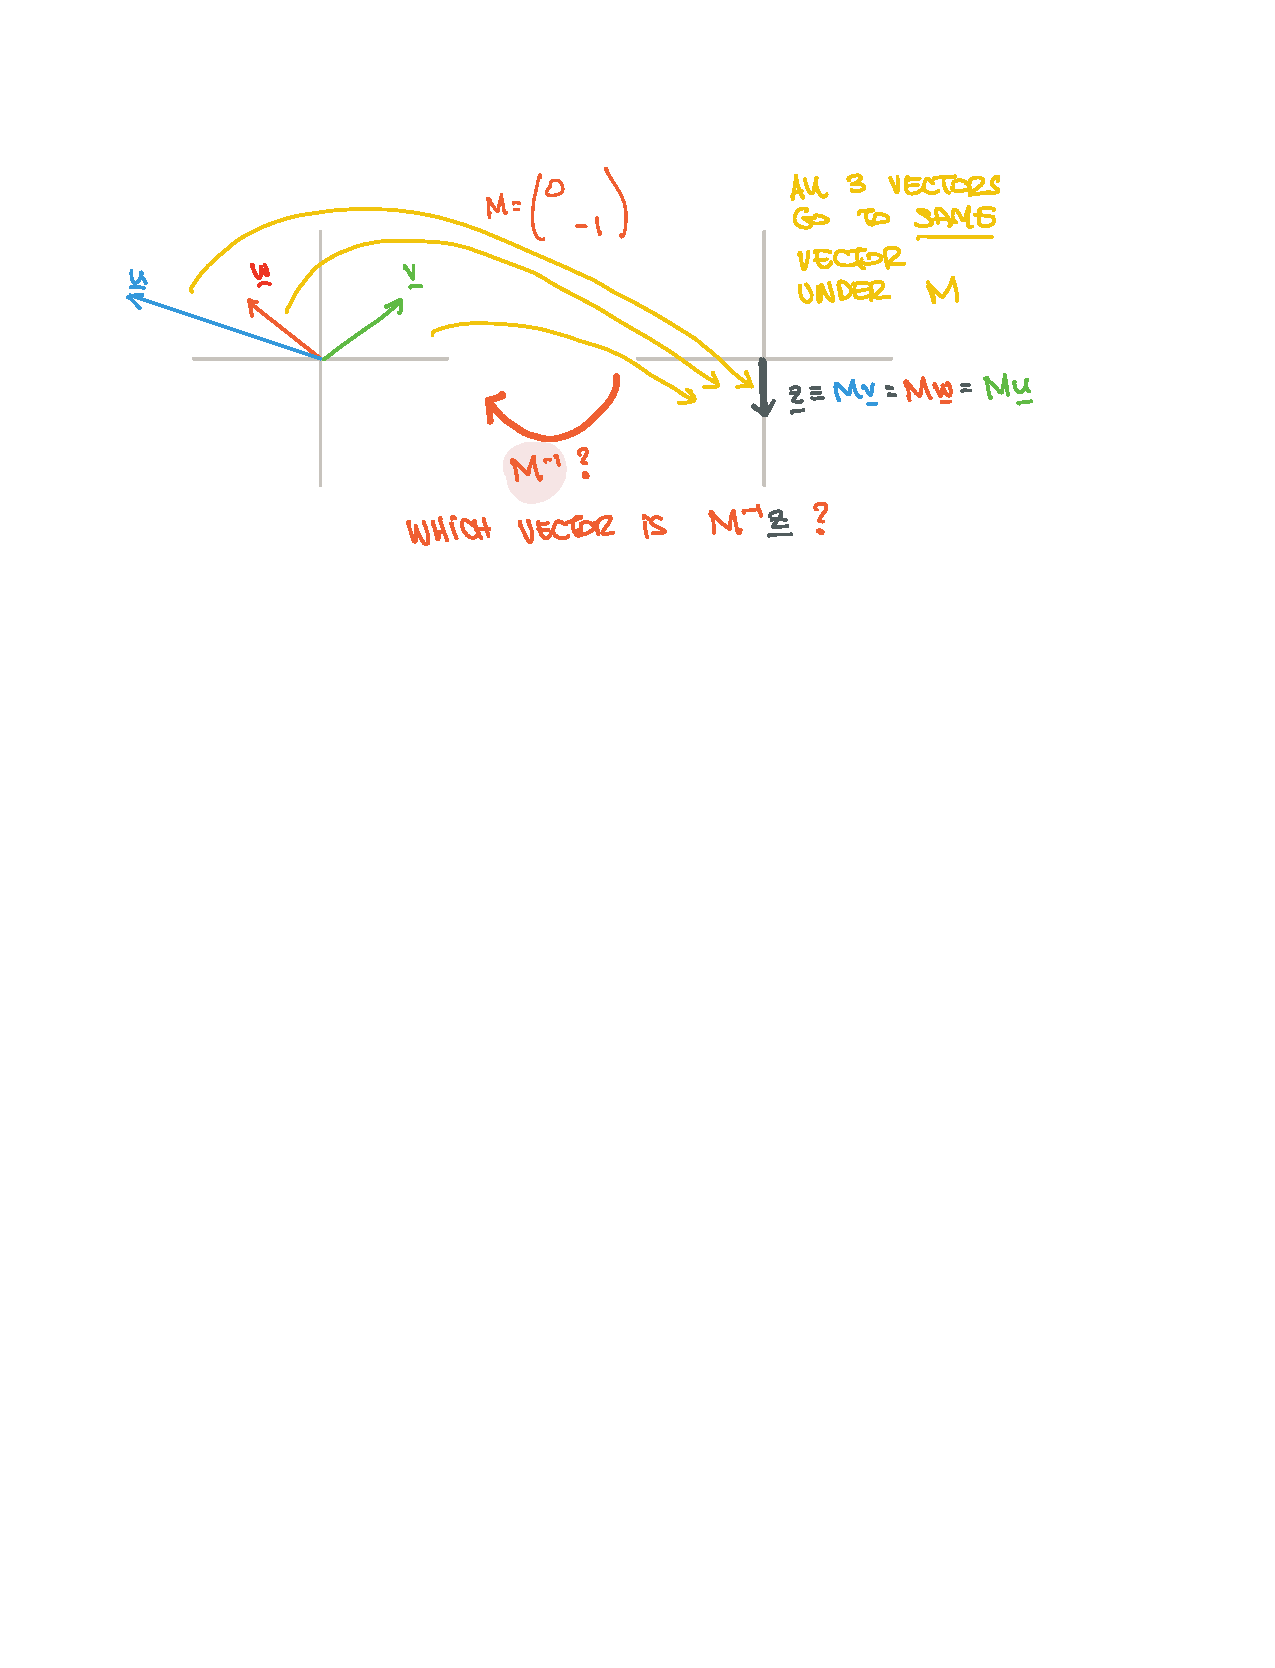
\includegraphics[width=.8\textwidth]{figures/maps_noninv.pdf}
    \caption{$M$ is a non-invertible matrix. We notice that there's no problem applying $M$ to vectors. The odd thing is that there are multiple vectors---$\vec{v}$, $\vec{w}$, and $\vec{u}$ in the picture---that all turn into the same vector, $M\vec{v} = M\vec{w}=M\vec{u}\equiv \vec{z}$. The problem shows up when we try to ``undo'' the transformation $M$ by applying $M\inv$ to $\vec{z}$. $M\inv\vec{z}$ should be a vector. Instead, we have at least three different valid options: $\vec{v}$, $\vec{w}$, and $\vec{u}$. This means that $M\inv$ is not a well defined linear map: it can send one vector $\vec{z}$ into many possible vectors. }
    \label{fig:map:M:no:inv}
\end{figure}
% 
Thinking of the matrix $M$ as a map, we see the the problem is one of uniqueness. A linear map should take each vector $\vec{v}$ into a single, well-defined vector $M\vec{v}$. $M$ is suspicious because it sends multiple different vectors to the \emph{same} vector, say $M\vec{v} = M\vec{w}$. That's fine. Each of $\vec{v}$ and $\vec{w}$ are sent to \emph{a} vector. The problem shows up when we try to take the inverse. If we write $\vec{z} = M\vec{v} = M\vec{w}$, we know that
\begin{align}
    (M\inv)\vec{z} = (M\inv)M\vec{v} &= \vec{v}
    &
    (M\inv)\vec{z} = (M\inv)M\vec{w} &= \vec{w} \ .
\end{align}
However, we assumed that $\vec{v} \neq \vec{w}$. This means makes the above line inconsistent. The inverse transformation is not defined. Bummer.

Fortunately, most of the \emph{dynamics} in physics \emph{is} invertible. That does not mean that we can ignore non-invertible matrices, though. Non-invertible matrices can be understood as \textbf{projections} onto a subspace. You can see this in the example in Fig.~\ref{fig:map:M:no:inv}. The map $M$ is essentially only using the information about the second component of its input vector and mapping it to just the second component of the output vector. That means that $M$ is really just a map to a one-dimensional subspace. In this way, the two dimensional vector space $\RR ^2$ is \textbf{projected} onto a one-dimensional subspace of $\RR ^2$. In that example, the one dimensional space is defined by vectors of the form
\begin{align}
    \vec{v} = 
    \begin{pmatrix}
    0\\ v^2    
    \end{pmatrix} \ .
\end{align}

Projections are really useful in physics. Sometimes you want to take a big vector space and only focus on a subspace that satisfy certain conditions. For example, it turns out that in nature you can have two types of massless matter particles: left-handed and right-handed according to their quantum spin in the direction of their motion. One may want to project onto only the space of left-handed particles because that is easier to deal with than the entire space. Because projections necessarily ``throw out'' information, they are non-invertible.\footnote{I think this was more intuitive to past generations of physicists. When you throw out a piece of paper, it ends up in a recycling plant and it gets torn up and is lost forever. Since the advent of computers, when you ``throw out'' a file, you can usually control/command-z and undo to bring it back.}

\begin{example}
One of the most curious puzzles in fundamental physics over the last half century is the black hole information paradox.\footnote{\url{https://www.quantamagazine.org/the-most-famous-paradox-in-physics-nears-its-end-20201029/}} One way of stating the paradox is the question of whether or not ``falling into a black hole'' is a \emph{projection} that throws out information. 
\end{example}

\subsection{Funny things you can do to matrices}
\label{sec:transpose:trace:det}

\subsubsection*{Transpose}

The \textbf{transpose} of a matrix is what happens when you `flip all the elements along the diagonal.' Given a matrix $M$, the transpose of $M$ is $M^T$ with components
\begin{align}
    (M^T)\aij{i}{j} &= M\aij{j}{i} \ .
    \label{eq:transpose:components}
\end{align}

\begin{example}
The following two matrices are transposes of each other.
\begin{align}
    M &= 
    \begin{pmatrix}
        9 & -3 & 2 \\
        2 & \pp 5 & 7 \\
        1 & \pp 0 & 3
    \end{pmatrix}
    &
    M^T &= 
    \begin{pmatrix}
        \pp 9 & 2 & 1 \\
        -3 & 5 & 0 \\
        \pp 2 & 7 & 3
    \end{pmatrix}
    \ .
\end{align}
\end{example}

This unusual operation will turn out to be rather useful for us. I leave the following cryptic statement: the transpose of a matrix is \emph{not} its inverse, but it does have a \emph{dual} relationship to the original matrix. Once we define a metric, we will be able to give a more rigorous definition for transpose. For now, let use take \eqref{eq:transpose:components} as the definition of something we can `do' to matrices. 


\subsubsection*{Trace}

The \textbf{trace} of a matrix $M$ is simply the sum of its diagonal components:
\begin{align}
    \Tr M = M\aij{i}{i} = M\aij{1}{1} + M\aij{2}{2} + \cdots \ .
\end{align}
It is not obviously meaningful from the perspective of $M$ being a linear transformation. However, it ends up being useful as as a mechanical procedure that one can do to matrices. The reason for this is something we will see soon: the trace of a matrix is unchanged under rotations. 

\subsubsection*{Determinants}

Here's another seemingly strange operation that you can do on a matrix. The determinant of a $2\times 2$ matrix is defined to be
\begin{align}
    \det M \equiv M\aij11 M\aij12 - M\aij12 M\aij21 \ .
\end{align}
Weird, right? Determinants for higher-dimensional square matrices can be defined recursively by taking specific linear combinations of sub-matrices. There are silly rules for this. There are fancy words for the sub-matrices (minors) and the appropriate sign for summing together those determinants (cofactors). Look, it's a mess. You should be able to calculate the determinant of a general $2\times 2$ matrix because it's easy. In case of national crisis, you should be able to calculate the determinant of a general $3\times 3$ matrix after consulting a reference to double check the signs. However, at this stage we will not make a big deal about determinants. I think engineering classes make a big deal about determinants because they can help with solving systems of linear equations using matrices---but \emph{that's not the kind of linear algebra we're doing in physics}.

\begin{example}\label{eg:determinant:of:diagonal}
The determinant of a diagonal matrix is simply the product of each of its diagonal elements. 
\end{example}

Determinants of a matrix are at least as curious as its trace because the determinant of a matrix turns out to also be unchanged under rotations. Furthermore, in multivariable calculus, the determinant shows up in the volume element. In fact, there is a formal definition of the determinant that comes from differential geometry where we use the determinant to rigorously define volumes of curved spaces. This sort of thing shows up in general relativity.
%
One way of starting to see why this is plausible is the observation that the determinant of a matrix $M$ is equal to the area of the parallelogram whose sides are given by the transformed basis vectors, $M\bas{e}_i$. We sketch this in two dimensions in Fig.~\ref{fig:determinant:map:area}. 
% 
\begin{figure}[tb]
    \centering
    \includegraphics[width=.8\textwidth]{figures/determinant_sketch.pdf}
    \caption{The transformation by $M$ of a unit square with sides $\bas{e}_i$ is a parallelogram with sides $M\bas{e}_i$. The determinant of $M$ is the area of the parallelogram. In more than three dimensions the shape is called a parallelpiped, which is a fun word to say.}
    \label{fig:determinant:map:area}
\end{figure}
% 
To prove this claim in two dimensions, we enclose the parallelogram into a box and start figuring out the area of various sub-shapes. Let $A_\text{r}$ be the area in the two red triangles, $A_\text{b}$ be the area in the two green triangles, and $A_\text{g}$ be the area of the two blue boxes. These areas are---accounting for the factor of two because there are two of each shape:
\begin{align}
    A_\text{r} &= M\aij 11 M \aij 21
    &
    A_\text{g} &= M\aij 22 M \aij 12
    &
    A_\text{b} &= 2 M\aij 12 M \aij 21 \ .
\end{align}
The total area of the large box is
\begin{align}
    A_\text{tot} &= (M\aij 11 + M\aij 12)(M\aij 22 + M\aij 21) 
    \\&= M\aij 11 M\aij 22 + 
    M\aij 11 M\aij 21 + 
    M\aij 12 M\aij 22 + 
    M\aij 12 M\aij 21 
    \\ &= 
    M\aij 11 M\aij 22 + 
    A_\text{r} + 
    A_\text{g}  + 
    \frac 12 A_\text{b} 
    \ . 
\end{align}
% 
\begin{figure}[tb]
    \centering
    \includegraphics[width=.8\textwidth]{figures/determinant_sketch2.pdf}
    \caption{Graphical aid for understanding the area of the parallelogram whose sides are $M\bas{e}_i$.}
    \label{fig:determinant:map:area:proof}
\end{figure}
% 
The area of the parallelogram is simply the area of the large box minus the areas of the non-parallelogram shapes, $A_\text{tot}- A_\text{r} - A_\text{g} - A_\text{b}$:
\begin{align}
    A_\text{parallelogram} =  M\aij 11 M\aij 22 - \frac 12 A_\text{b}  = M\aij 11 M\aij 22  - M\aij 12 M\aij 21  = \det M \ .
    \label{eq:det:is:area:parallelogram}
\end{align}
And so we have shown the result in a simple case: determinants are related to areas. Specifically, we see that the determinants are related to the areas (volumes) of parallelograms (parallelpipeds) with sides $M\bas{e}_i$. 

This interpretation of determinants as volumes\footnote{I now say `volumes' instead of `area' because what follows is general to any dimension of space.} also motivates some further expressions for the determinant of the product of matrices and the determinant of the inverse of a matrix. If we perform subsequent transformations with two matrices, $N$ and $M$, then the unit parallelpiped is first mapped to a parallelpiped of volume $\det N$. When we apply the second matrix $M$, this intermediate parallelpiped is mapped to a third parallelpiped whose volume is rescaled by $\det M$. The resulting volume is $(\det N)(\det M)$. We thus deduce that the determinant of a product of matrices is the product of the determinants of each matrix:
\begin{align}
    \det NM = (\det N)(\det M) \ . 
    \label{eq:det:of:product}
\end{align}
Going further, because $M M\inv = \one$, we have
\begin{align}
    \det M M\inv &= (\det M)(\det M\inv ) = \det\one = 1 
    & \Rightarrow&
    &
     \det M\inv &= \frac{1}{\det M} \ .
    % {eq:det:of:product}
    \label{eq:det:of:inverse}
\end{align}
We have been deliberately hand-wavy to motivate thesse relations for determinants. If we were to be more rigorous, the are rather tricky to prove, though you can do them by brute force by calculating components. 



\subsection{Matrices that aren't square: maps between vector spaces}

You may be wondering why all of our linear transformations are square. After all, you have probably seen rectangular matrices where the number of rows does not equal the number of columns. For example
\begin{align}
    W = 
    \begin{pmatrix}
        1 & \pp 2 &-6 & 7 \\
        6 & -3 & \pp 3 & 0
    \end{pmatrix} \ .
\end{align}
Just by looking at this, you can tell that $W$ acts on some kind of vector with four components and outputs a vector with two components. Assuming these vectors are part of $\RR ^4$ and $\RR ^2$ respectively, this means that $W$ is a map from $\RR ^4$ to $\RR ^2$, or
\begin{align}
    W:\; \RR ^4 \;\to \; \RR ^2 \ .
\end{align}
Non-square matrices are maps between different vector spaces. In this course we will have very little to say about non-square matrices. The type of linear algebra that comes up over and over again in physics are transformations from some vector space $V$ to itself.\footnote{To be more technically precise: the maps tend to be between vector spaces $V$ and $V'$ that are isomorphic to one another, $V\cong V'$. This means that the vector spaces may be different, but there is a unambiguous translation between the two.} 

The one thing we have observed about non-square matrices is that the number of columns is the maximum dimensionality of the input space, and the number of rows is the maximum dimensionality of the output space.\footnote{Why do we specify `maxmimum'? You could imagine a vector space that is two dimensional but happens to be written in a silly way as three-component vectors. For example, we could consider the space of vectors spanned by the $x$- and $y$-basis vectors but written as three component vectors in $\RR ^3$. That space is two dimensional, but the vectors have three components---one of which is always zero.} The dimensionality tells us about how much information is in a vector. A three-dimensional vector space has ``three numbers worth'' of information, the three components relative to a basis. This means that:
\begin{enumerate}
    \item If the number of columns is larger than the number of rows, then the output of the transformation may have less information than the input. For example, two different input vectors may map to the same output vector.
    \item If the number of rows is larger than the number of columns, then input of the transformation may not be able to encode enough information to populate every possible vector in the output space. For example, there may be vectors $\vec{v}_\text{out}$ in the output space that cannot be written as $W\vec{u}_\text{in}$. 
\end{enumerate}
There are some fancy words that are associated with these ideas. The \textbf{kernel}\footnote{The word kernel is really annoying here because it shows up in another place in the theory of distributions. Much to my chagrin, we will argue that distributions are an ingredient in the linear algebra of infinite dimensional vector spaces. This means that there is a place later in this course where the word \emph{kernel} will come up again but will mean something completely unrelated.} of a transformation $M$ is the set of all vectors $\vec{v}$ such that $M\vec{v} = 0$. The \textbf{image} of a transformation is the set of all vectors $\vec{v}$ that can be obtained by acting with the transformation $M$, that is: there is some $\vec{u}$ such that $\vec{v} = M\vec{u}$.
\begin{exercise}
Using the definition of a vector space, show that the kernel of $M$ and the image of $M$ are vector spaces. 
\end{exercise}

From this, we have argued that if $W: V_1 \to V_2$ is a linear transformation between two different vector spaces of different dimension, then 
\begin{enumerate}
    \item If the dimension of $V_1$, $\text{dim}\,V_1$, is larger than the dimension of $V_2$, $\text{dim}\,V_2$, then the kernel of $W$ contains more than just the zero vector.
    \item Alternatively, if $\text{dim}\,V_2 > \text{dim}\,V_1$, then the image of $W$ is a subspace of $V_2$ that does not contain all of $V_2$. 
\end{enumerate}

% \subsection{More Jargon}

\section{Rotations}
\label{sec:rotations}

Rotations are a special class of transformations. We wait until Section~\ref{sec:metric:spaces} to really appreciate why rotations are special. For now, you may rely on your ordinary intuition for what it means to \emph{rotate} something. If a vector is an arrow---\emph{I know, this is the kindergarden picture of vectors}---then you rotate it by pinning its tail to the origin and then moving the arrowhead while leaving the length unchanged. 

A more important notion of rotation is the idea of a change of basis between `nice' basis vectors---a notion that we formalize when we have a dot (inner) product. The physical manifestation of this is the idea of a \emph{passive} rotation. This corresponds in physics to a \emph{change in reference frame}. We illustrate this in Fig.~\ref{fig:passive:rotation}. 
\begin{figure}[tb]
    \centering
    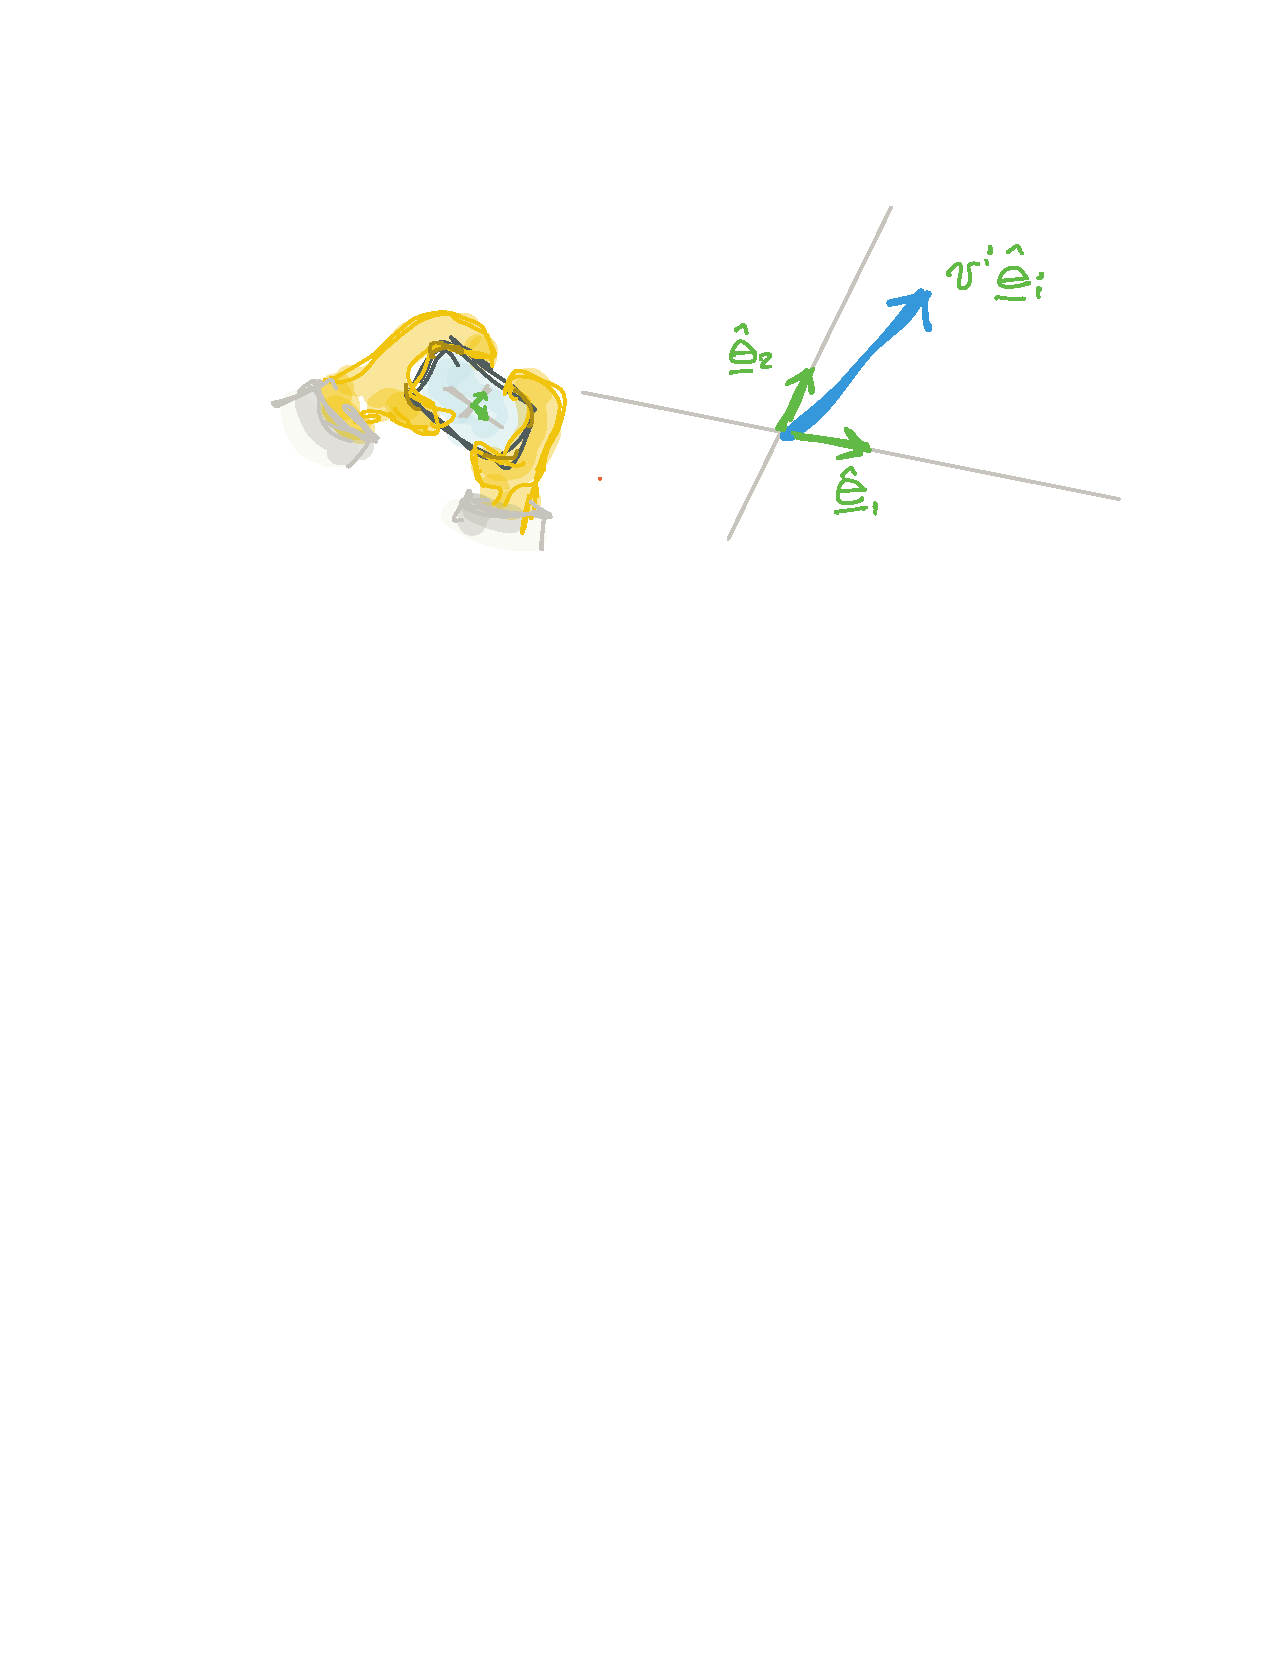
\includegraphics[width=.43\textwidth]{figures/rotate_1.pdf}
    \quad\quad
    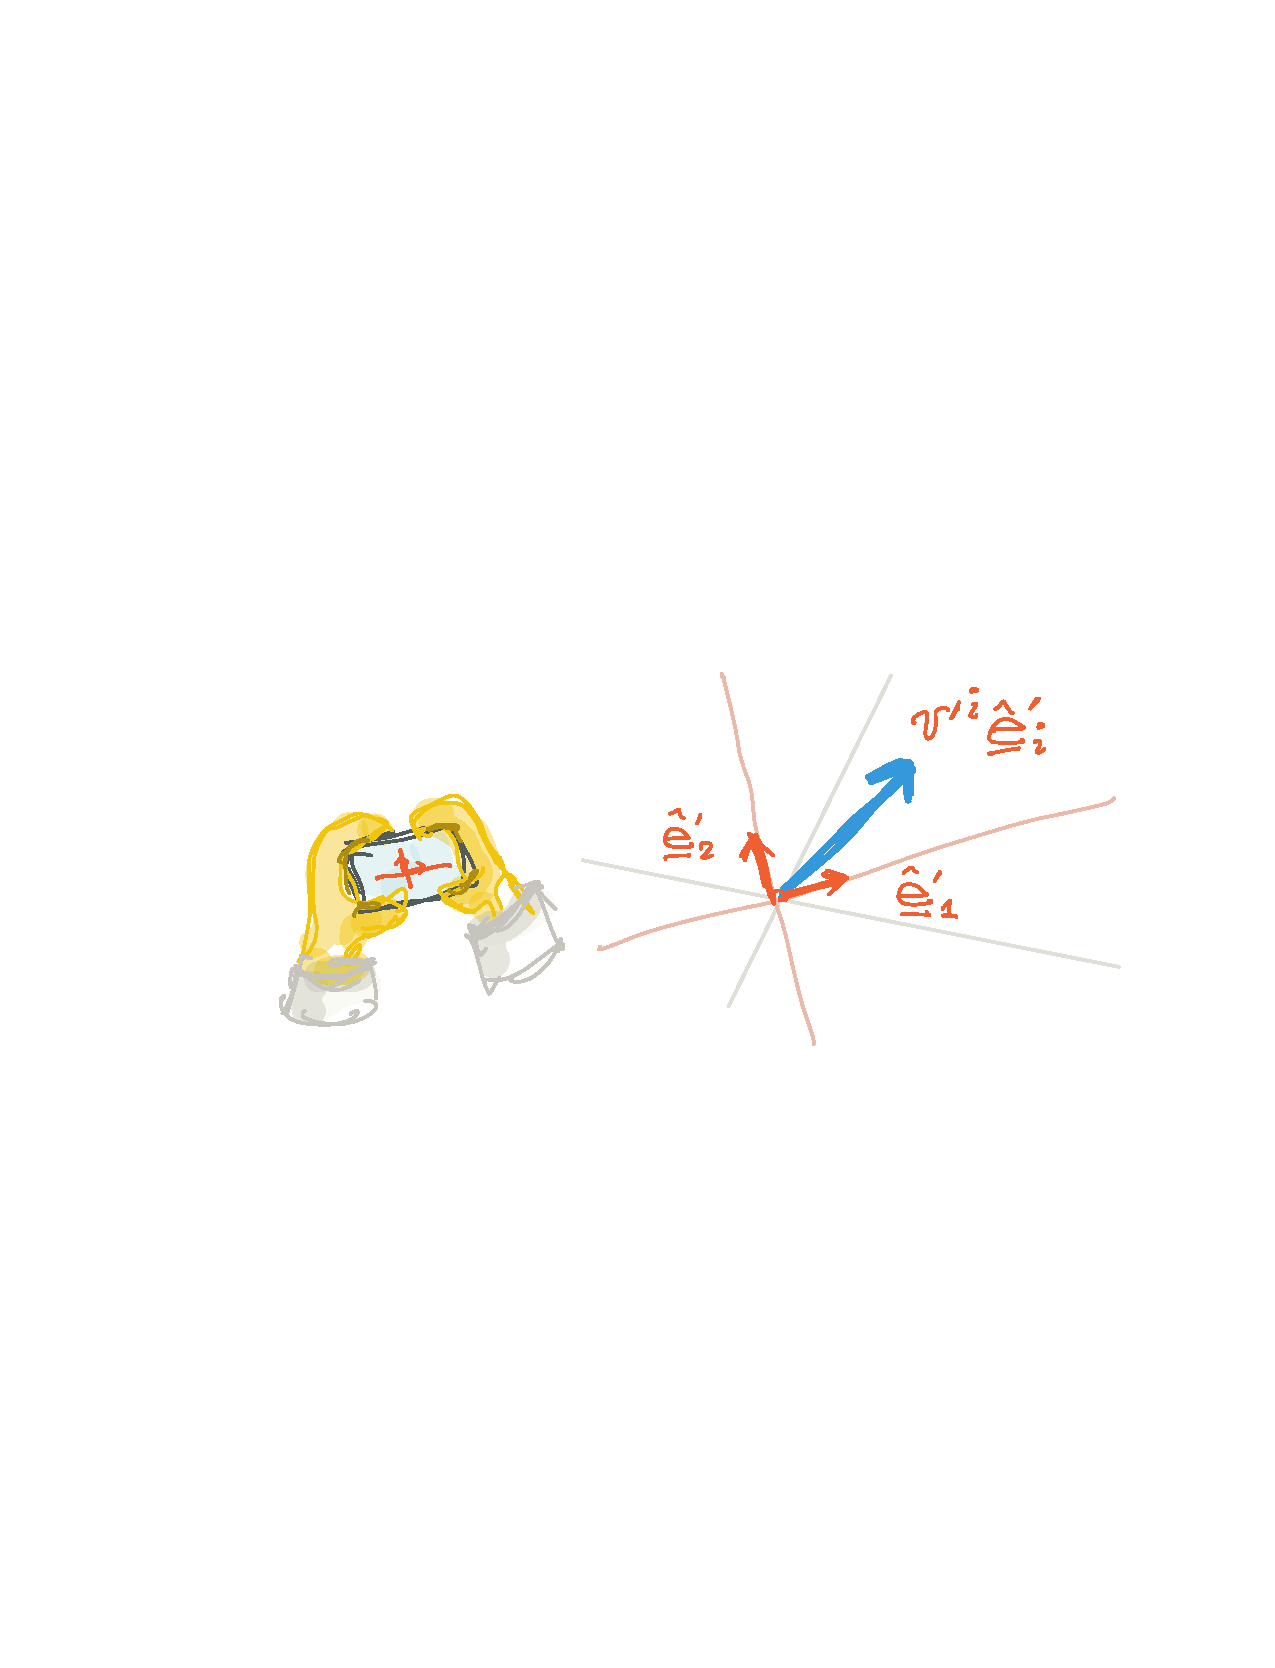
\includegraphics[width=.43\textwidth]{figures/rotate_2.pdf}
    \caption{Example of a passive rotation. You are looking at a vector $\vec{v}$ through your phone. The image on your phone has a natural orientation for a basis $\bas{e}_i$ and the components of $\vec{v}$ in this basis are $v^i$. You could also rotate your phone, leaving the vector $\vec{v}$ untouched. The new basis vectors are $\bas{e}_i'$; they are different from $\bas{e}_i$ because your phone has changed orientation. With respect to the new basis, the same vector $\vec{v}$ now has components $v'^i$.}
    \label{fig:passive:rotation}
\end{figure}


\subsection{Rotations in Two-Dimensions}

In two dimensions, there is only one class of rotation matrix. It has one parameter, $\theta$, the amount that one is rotating. We conventionally measure rotations in the counter-clockwise direction. Rotations are linear transformations, and thus are represented by matrices. The form of a rotation matrix in two dimensions is\footnote{By convention we define a rotation by $\theta$ to be in the counter-clockwise direction.}
\begin{align}
    R(\theta) = 
    \begin{pmatrix}
        \cos\theta & - \sin\theta \\
        \sin\theta & \pp \cos \theta
    \end{pmatrix}
    =
    \begin{pmatrix}
        c_\theta & - s_\theta \\
        s_\theta & \pp c_\theta
    \end{pmatrix}\ ,
    \label{eq:rotation:matrix:2D}
\end{align}
where on the right we have introduced some shorthand for the trigonometric functions. The key relation of the trigonometric functions is
\begin{align}
    \sin^2\theta + \cos^2\theta = c_\theta^2 + s_\theta^2 = 1 \ .
\end{align}

The inverse of a rotation is simply is simply a rotation in the opposite direction. This means that the inverse of the rotation matrix $R(\theta)$ is simply $R\inv(\theta) = R(-\theta)$. Because cosine is an even function and sine is an odd function, this means
\begin{align}
R\inv(\theta) = 
\begin{pmatrix}
        \pp c_\theta &  s_\theta \\
        - s_\theta &  c_\theta
    \end{pmatrix} 
    = 
    R(\theta)^T
    \ .
\end{align}
The last equality may be a little surprising, but it is of utmost significance. The inverse of a rotation is the transpose of the original rotation. 

\begin{exercise}
Check component-by-component that $R(\theta)R\inv(\theta) = \one $ using the expressions above. One may directly show that for each of the four combinations of $i$ and $j$,
\begin{align}
    R(\theta)\aij{i}{k} \, R\inv(\theta)\aij{k}{j} &= \delta^i_j  \ .
\end{align}
% For each of the four combinations of $i$ and $j$. 
\end{exercise}

\begin{example}
A physically motivated (and much simpler) way of writing the inverse rotation is to recall that to undo a counterclockwise rotation by angle $\theta$, one does a clockwise rotation by $\theta$. This is simply a counterclockwise rotation by angle $-\theta$. Thus
\begin{align}
    R\inv(\theta) = R(-\theta)
    =
    \begin{pmatrix}
        \cos(-\theta) & \sin(-\theta) \\
        \sin(-\theta) & \pp \cos(-\theta)
    \end{pmatrix}
    =
    \begin{pmatrix}
        \pp c_\theta &  s_\theta \\
        - s_\theta &  c_\theta
    \end{pmatrix}  
    =
    R(\theta)^T
    \ .
\end{align}
We used the fact that sine is odd, $\sin(-\theta) = -\sin\theta$ and cosine is even, $\cos(-\theta) = -\cos\theta$.
\end{example}

We have thus proven the existence of an inverse rotation by explicitly constructing the inverse of the rotation matrix. This makes sense: rotations are ``nice'' transformations that clearly do not lead to a loss of information. After all, the rotation of a vector is simply what you would see by looking at the vector and tilting your head a little. This remark will lead us to the idea of a \emph{passive} transformation. 

\begin{exercise}
Consider a point on the Cartesian plane $(x,y)$. Derive the rotation matrix \eqref{eq:rotation:matrix:2D} by determining the rotated coordinates $(x',y')$ as a function of $x$, $y$, and the rotation angle $\theta$. I suggest writing $x=r\cos\phi$ and $y=r\sin\phi$. Then use the fact that under a rotation, radius stays the same and angles add. Thus
\begin{align}
     x' &= r\cos(\phi+\theta)
     &
     y' &= r\sin(\phi+\theta) \ .
 \end{align}
Then invoke the angle addition formulae for trigonometric functions. 
\end{exercise}

\begin{exercise}
Show that the determinant of the $2\times 2$ rotation matrix is one.
\end{exercise}


\subsection{Transformation of Vectors}

What can we do with a rotation matrix? Why, rotate vectors, of course! In this respect, $R(\theta)$ is just like any other linear transformation. Here it is in matrix notation. A vector $\vec{v}$ transforms into a vector $\vec{v}' = R(\theta)\vec{v}$ with components
\begin{align}
    \begin{pmatrix}
        v'^1\\ v'^2
    \end{pmatrix}
    =
    \begin{pmatrix}
        \cos\theta & - \sin\theta \\
        \sin\theta & \pp \cos \theta
    \end{pmatrix}
    \begin{pmatrix}
        v^1 \\ v^2
    \end{pmatrix}
    &= 
    \begin{pmatrix}
        \cos\theta\; v^1 - \sin\theta\; v^2\\
        \sin\theta\; v^1 + \cos\theta\; v^2
    \end{pmatrix} \ .
\end{align}
Here it is in component notation:
\begin{align}
    v'^i =
    \left(R(\theta)v\right)^i &= 
    R(\theta)\aij{i}{j}v^j \ .
    \label{eq:col:vector:rotation}
\end{align}
We can observe something significant:
\begin{bigidea}\label{idea:upper:index:rotates:with:R}
A generic component of a vector has an upper index, $v^i$. The component of the rotated vector under a rotation $R(\theta)$ has generic component $R(\theta)\aij{i}{j}v^j$. That is: we take the rotation matrix and contract its second index (which is lower) with the upper index of the vector. 
\end{bigidea}



Thus far, rotations are just some linear transformation. We have not yet defined the features that make rotations special in Euclidean space. Indeed: we are not in Euclidean space yet, we are simply in $\RR ^3$, the class of vector spaces described by three real numbers. Once we have a metric (dot product) then we can say that rotations preserve the dot product. A rotated vector does not change length under a rotation. Angles between vectors---which we saw in \eqref{eq:cos:theta:in:R3} are also defined by the dot product---are also unchanged under rotations. 

\subsection{Transformation of numbers}\label{sec:rotation:of:numbers}

Numbers, also known as scalars, do not transform under rotations. Here's a useful phrase: we say that numbers are \textbf{invariant} under rotations. Here's a prescient way of saying the same thing a third time:

\begin{bigidea}\label{idea:no:index:rotates:without:R}
An object with \emph{no} indices does not transform under rotations.
\end{bigidea}

\subsection{Transformation of Row Vectors}

What about row vectors? Row vectors also transform under rotations. In matrix notation the transformation looks like this: $\row{w}\to \row{w}' = \row{w}R(\theta)\inv$,
\begin{align}
    \begin{pmatrix}
        w'_1 & w'_2
    \end{pmatrix}
    &=
    \begin{pmatrix}
        w_1 & w_2
    \end{pmatrix}
    \begin{pmatrix}
        \pp \cos\theta & \sin\theta \\
        - \sin\theta & \cos \theta
    \end{pmatrix} \ .
\end{align}
In component notation:
\begin{align}
    w'_i = (wR(\theta)\inv)_i = w_j \left(R(\theta)\inv\right)\aij{j}{i} 
    = \left(R(\theta)\inv\right)\aij{j}{i} w_j  
    \ .
    \label{eq:row:vector:rotation}
\end{align}
One can of course write the components of $R(\theta)\inv$ in terms of those of $R(\theta)$, but it turns out to be convenient to keep track of when we have $R(\theta)$ versus $R(\theta)^{-1}$.  Observe that by the usual rules of matrix multiplication, the row vector needs to be on the left of the matrix. That is, $\row{w}R(\theta)\inv$ makes sense, while $R(\theta)\inv \row{w}$ does not. However, on the right side of \eqref{eq:row:vector:rotation} we have done something slippery: we have written the \emph{component} $\left(R(\theta)\inv\right)\aij{j}{i}$ to the \emph{left} of the \emph{component} $w_j$. This is totally allowed, since \emph{components are just numbers}. They carry no vector-y (``tensorial'') structure themselves. Indeed, this is one of the benefits of component notation. 

At this point you should be very perplexed: \emph{why} does the row vector transform \emph{oppositely} to the column vector? Thus far we have simply stated that ``this is the way.\footnote{\url{https://knowyourmeme.com/memes/this-is-the-way}}'' However, consider the action of a row vector on a vector: $\row{w}\vec{v}$. This is simply a number, and as you know from Section~\ref{sec:rotation:of:numbers}, \emph{numbers do not transform under rotations}. Is this consistent with $\row{w}$ and $\vec{v}$ transforming? Let us quickly confirm. In matrix notation, we have:
\begin{align}
    \row{w}\vec{v}\to \row{w}'\vec{v}' = \row{w} R(\theta)\inv\, R(\theta) \vec{v} = \row{w}\vec{v} \ .
    \label{eq:row:col:contract:transformation}
\end{align}
Here we have simply used $R\inv R = \one $. We can write the same thing in component notation;
\begin{align}
    w'_i v'^i = \left(R(\theta)\inv\right)\aij{k}{i} R(\theta)\aij{i}{j} w_k v^j = \delta^k_j w_k v^j = w_kv^k \ .
\end{align}
We used \eqref{eq:inverse:matrix:definition} and \eqref{eq:kronecker:delta:action} to write the product of a matrix with its inverse in terms of the Kronecker $\delta$, and then to use the Kronecker $\delta$ to collapse the lower $j$ index into a lower $k$ index.  Let us be clear that we were able to `pull out' the \emph{components} of the rotation matrices because they are simply numbers. Further, let us be clear that the components of $R(\theta)$ and $R(\theta)\inv$ are contracted in specifically the right way to yield the Kronecker $\delta$:
\begin{align}
    \left(R(\theta)\inv\right)\aij{k}{i} R(\theta)\aij{i}{j} = \delta^k_j \ .
\end{align}

What we see is that the transformation law for row vectors, \eqref{eq:row:vector:rotation}, is precisely what it needs to be so that the number $\row{w}\vec{v}$ is invariant under a rotation. Further, we observe something significant:
% 
\begin{bigidea}\label{idea:lower:index:rotates:with:Rinv}
A generic component of a row vector has a lower index, $w_i$. The component of the rotated row vector under a rotation $R(\theta)$ has generic component $(R(\theta)\inv)\aij{j}{i}w_j$. That is: we take the \emph{inverse} rotation matrix and contract its \emph{first} index (which is upper) with the lower index of the vector. 
\end{bigidea}


\subsection{Transformation of Matrices}
\label{sec:transformation:of:matrices}

Do matrices transform under a rotation? Matrices are linear maps from vectors to vectors, so we know that $M\vec{v}$ is a vector. That means that $M\vec{v}$ transforms the way any other vector transforms under a rotation $R(\theta)$:
\begin{align}
    M\vec{v} \to (M\vec{v})' &= R(\theta)\, M\vec{v} 
    &
    (M\vec{v})'^i  &= R(\theta)\aij{i}{j} M\aij{j}{k}v^k 
    \ .
\end{align}
Note that $R(\theta)M \neq M R(\theta)$ because these are matrices. Similarly, on the right-hand side 
\begin{align}
    R(\theta)\aij{i}{j} M\aij{j}{k}v^k \neq 
    M\aij{i}{j} R(\theta)\aij{j}{k} v^k \ ,
\end{align}
although it \emph{is} true that (note the difference in indices compared to above)
\begin{align}
    R(\theta)\aij{i}{j} M\aij{j}{k}v^k =
    M\aij{j}{k} R(\theta)\aij{i}{j} v^k \ .
\end{align}
In the spirit of \eqref{eq:row:col:contract:transformation}, we would like to write the transformed vector $(M\vec{v})'$ in terms of a transformed matrix $M'$ acting on the transformed vector $\vec{v}'$. We define the transformed matrix $M'$ this way:
\begin{align}
    M' \vec{v}' &= R(\theta)\, M\vec{v} = R(\theta)\, M R(\theta)\inv \vec{v}'   \ .
\end{align}
In component notation, this is:
\begin{align}
    (M')\aij{i}{\ell} (v')^\ell &= 
    R(\theta)\aij{i}{j}
    M\aij{j}{k}
    (R(\theta)\inv)\aij{k}{\ell}
    (v')^\ell \ .
    \label{eq:deriving:Mprime:rotation:cancel:vp}
\end{align}
We have been very clever and chose to write the dummy indices on the left-hand side to match the dummy indices of the last contraction on the right hand side. We now claim that we can ``cancel the $(v')^\ell$'' on both sides of this equation. This can be a very subtle point the first time you see it. The crux of the argument is that \eqref{eq:deriving:Mprime:rotation:cancel:vp} holds \emph{for any} vector $\vec{v}'$, and thus the equality cannot depend on the components of $\vec{v}'$. That means that the equality is really an equality between the matrices acting on $\vec{v}'$. To appreciate this subtlety, please see Example~\ref{ex:cancel:vector:in:matrix:equation} below.

Having performed the slick step of canceling out $(v')^\ell$, we have the expression for the components of the transformed matrix, $M'$:
\begin{align}
    (M')\aij{i}{\ell}&= 
    R(\theta)\aij{i}{j}
    M\aij{j}{k}
    (R(\theta)\inv)\aij{k}{\ell}
    = 
    R(\theta)\aij{i}{j}
    (R(\theta)\inv)\aij{k}{\ell}
    M\aij{j}{k}
    &
    M' = R(\theta) M R(\theta)\inv
    \ .
    \label{eq:deriving:Mprime:components}
\end{align}
Observe that the rotation matrices in $M'$ are precisely what they must be to ensure that the number $\row{w}M\vec{v}$ is invariant:
\begin{align}
    \row{w}M\vec{v} \to \row{w}'M'\vec{v}' = 
    \row{w} R(\theta)\inv R(\theta) \; M\; R(\theta)\inv R(\theta)\vec{v}
    =
    \row{w}M\vec{v} \ .
\end{align}
We recognize two pairs of matrix--inverse matrix products. We could write out the long expression in terms of indices, but I fear we would run out of letters. What is catches our eye in \eqref{eq:deriving:Mprime:components} is the continuation of the string of ideas in \bigidearefs~\ref{idea:upper:index:rotates:with:R}, \ref{idea:no:index:rotates:without:R}, and \ref{idea:lower:index:rotates:with:Rinv}:
% 
\begin{bigidea}\label{idea:matrix:index:rotates:with:R:Rinv}
A generic component of a matrix has an upper index and a lower index, $M\aij{i}{j}$. The generic component of the rotated matrix under a rotation $R(\theta)$ is $R(\theta)\aij{i}{k}\, (R(\theta)\inv)\aij{\ell}{j}\, M\aij{k}{\ell}$. We contract the upper index of $M$ with the lower index of $R(\theta)$ and we contract the lower index of $M$ with the upper index of $R(\theta)\inv$. The remaining indices of $R(\theta)$ and $R(\theta)\inv$ are the indices of $(M')\aij{i}{j}$.
\end{bigidea}









\begin{example}\label{ex:cancel:vector:in:matrix:equation}
Consider the case $M\vec{v} = N\vec{v}$ for the case $\vec{v} = \bas{e}_1$. This sets two vectors equal:
\begin{align}
    \begin{pmatrix}
        M\aij 11  & M\aij 12 \\
        M\aij 21  &  M\aij 22
    \end{pmatrix}
    \begin{pmatrix}
        1 \\ 0
    \end{pmatrix}
    &= 
    \begin{pmatrix}
        M\aij 11 \\ M\aij 21
    \end{pmatrix} 
    &
    \begin{pmatrix}
        N\aij 11  & N\aij 12 \\
        N\aij 21  & N\aij 22
    \end{pmatrix}
    \begin{pmatrix}
        1 \\ 0
    \end{pmatrix}
    = 
    \begin{pmatrix}
        N\aij 11 \\ N\aij 21
    \end{pmatrix} 
    \ .
    \label{eq:ex:cancel:vector:in:matrix:eq:1}
\end{align}
We see that the equality is satisfied if only the first columns of $M$ and $N$ match. The second columns could differ, say $M\aij 12 \neq N\aij 12$, and so we cannot conclude that $M=N$. However, if we say that $M\vec{v} = N\vec{v}$ for \emph{every} vector $\vec{v}$, then we could also check $\vec{v} = \bas{e}_2$ to find
\begin{align}
    \begin{pmatrix}
        M\aij 11  & M\aij 12 \\
        M\aij 21  &  M\aij 22
    \end{pmatrix}
    \begin{pmatrix}
        0 \\ 1
    \end{pmatrix}
    &= 
    \begin{pmatrix}
        M\aij 12 \\ M\aij 22
    \end{pmatrix} 
    &
    \begin{pmatrix}
        N\aij 11  & N\aij 12 \\
        N\aij 21  & N\aij 22
    \end{pmatrix}
    \begin{pmatrix}
        0 \\ 1
    \end{pmatrix}
    = 
    \begin{pmatrix}
        N\aij 12 \\ N\aij 22
    \end{pmatrix} 
    \ .
    \label{eq:ex:cancel:vector:in:matrix:eq:2}
\end{align}
The combination of \eqref{eq:ex:cancel:vector:in:matrix:eq:1} and \eqref{eq:ex:cancel:vector:in:matrix:eq:2} means that $M=N$.
\end{example}
\begin{exercise}
Explain why it is sufficient to show $M\bas{e}_i = N\bas{e}_i$ for both basis vectors in Example~\ref{ex:cancel:vector:in:matrix:equation} to prove the equality of $M$ and $N$ given the relation $M\vec{v} = N\vec{v}$ for any $\vec{v}$. How do you know that the equality holds for $\vec{v} \neq \bas{e}_i$? Your argument should invoke the notion of linear combinations and linearity.
\end{exercise}





\subsection{Transformation of Tensors}


Why stop at two indices? A \textbf{tensor} is, in general, an object with indices associated with a vector space. The tensor can have any number of indices. Each index is either upper (column-like) or lower (row-like). A vector is a tensor with one upper index. A row vector is a tensor with one lower index. A matrix is a tensor whose first index is upper, and whose second index is lower. A number is a tensor with no indices.  A tensor with three indices can be written as a cube of components in the same way that a matrix can be written as a table of components. Tensors with more than three indices are hard to write down in ``matrix form.'' It's a good thing we've been spending all this time developing index notation, right?
\begin{example}
The \textbf{moment of inertia} tensor is a tensor with two indices, like a matrix. However, unlike a matrix, the moment of inertia tensor has two upper indices. This means it is rather different than a matrix. We now explain how they are different.
\end{example}

The significance of a tensor and its indices are that the indices tell us how the tensor transforms under rotations. This is the culmination of \bigidearefs~\ref{idea:upper:index:rotates:with:R}, \ref{idea:no:index:rotates:without:R}, \ref{idea:lower:index:rotates:with:Rinv}, and \ref{idea:matrix:index:rotates:with:R:Rinv}. We now \emph{define} the generalization of these ideas to a tensor, which is a pretty good working definition for what a tensor is:
\begin{bigidea}\label{idea:tensor:rotation}
A tensor with $p$ upper indices and $q$ lower indices is called a \textbf{rank}~$(p,q)$ tensor. For convenience of writing components using ellipses, let us write all of the upper indices first and then all of the lower indices last---this does not have to be the case, but the following result will hold. Under a rotation $R(\theta)$, the components of a tensor $T$ transform as
\begin{align}
    T^{i_1\cdots i_p}_{\phantom{i_1\cdots i_p}j_1\cdots j_q} \to 
    (T')^{i_1\cdots i_p}_{\phantom{i_1\cdots i_p}j_1\cdots j_q}
    = 
    \left[\prod_{p}
            % R(\theta)\aij{i_1}{k_1}\cdots 
            R(\theta)\aij{i_p}{k_p}\right]
    \left[\prod_{q}
            % (R(\theta)\inv)\aij{\ell_1}{j_1}\cdots 
            (R(\theta)\inv)\aij{\ell_q}{j_q}\right]
    T^{i_1\cdots i_p}_{\phantom{i_1\cdots i_p}j_1\cdots j_q}  \ .
    \label{eq:transformation:of:tensor}
\end{align}
\end{bigidea}
\begin{example}
The matrix $T\aij{ij}{k}$ transforms as
\begin{align}
    T\aij{ij}{k} \to 
    R(\theta)\aij{i}{\ell}
    R(\theta)\aij{j}{m}
    (R(\theta)\inv)\aij{n}{k}
    T\aij{\ell m}{n} \ .
\end{align}
\end{example}

\begin{exercise}
The moment of inertia tensor has components $I^{ij}$ with $i$ and $j$ taking values from 1 to 3. How does the moment of inertia tensor transform under a three-dimensional rotation $R$? (A three dimensional rotation is described by three angles. We shall be lazy and suppress those arguments altogether.) Compare this transformation law to that of a matrix, $M\aij{i}{j}$. This difference is why we say ``moment of inertia \emph{tensor}'' and not `moment of inertia matrix.'
\end{exercise}

A large part of physics is written in tensor notation.\footnote{As a curious side note, there is a graphical way of writing tensors called birdtracks. You can learn more about it at \url{https://birdtracks.eu}, or in Roger Penrose's book \emph{Road to Reality}. The notation is quite fetching, but ultimately I have not found it to be significantly more useful than indices.} This subsection finally gives a working definition for what a tensor is and hints at why it may be significant: it is an object that transforms in a prescribed way under rotations. Because rotations are related to changes in reference frame, tensors are objects where measuring the components in one frame allows us to predict the components that are measured by other observers. 

\subsection{Rotations in Three-Dimensions}

In $\RR ^3$ there are three different axes about which we can perform a rotation. These roughly correspond to three rotation matrices:
\begin{align}
    R_1(\theta_1)
    &=
    \begin{pmatrix}
        1 & 0 & \pp 0 \\
        0 & \text{c}_{\theta_1} & -\text{s}_{\theta_1} \\
        0 & \text{s}_{\theta_1} & \pp \text{c}_{\theta_1}
    \end{pmatrix}
    &
    R_2(\theta_2)
    &=
    \begin{pmatrix}
        \pp \text{c}_{\theta_2} & 0 & \text{s}_{\theta_2} \\
        \pp 0 & 1 & 0 \\
        -\text{s}_{\theta_2} & 0 & \text{c}_{\theta_2}
    \end{pmatrix}
    &
    R_3(\theta_3)
    &=
    \begin{pmatrix}
        \text{c}_{\theta_3} & -\text{s}_{\theta_3} & 0 \\
        \text{s}_{\theta_3} & \pp\text{c}_{\theta_3} & 0 \\
        0 & \pp 0 & 1
    \end{pmatrix} \ .
    \label{eq:rotation:matrix:basic}
\end{align}
You can see how these break down into two-dimensional rotations along each respective axis. If that is not obvious, please do the following exercise.
\begin{exercise}
Write the transformation of a three-component vector $\vec{v}$ with components $v^i$ under reach of the transformations in \eqref{eq:rotation:matrix:basic}. 
\end{exercise}
Additional rotations are produced by taking products of $R_1$, $R_2$, and $R_3$ by appropriate amounts. The properties of these rotations are outside the scope of our course, but their study is a big part of physics and is known as the \emph{representation theory of Lie groups}. If you want to do a deeper dive into rotation matrices in three dimensions, I recommend Howie Haber's lecture notes for Physics 216 at \acro{UCSC}\footnote{\url{http://scipp.ucsc.edu/~haber/ph216/rotation_12.pdf}}. 


All this is to say that there are more options for rotations in three dimensions. Given a particular rotation, $R$, then the tensor transformation rule in \bigidearef~\ref{idea:tensor:rotation} holds. In fact, one can start to piece together what a rotation in even higher dimensions looks like. You extend the list \eqref{eq:rotation:matrix:basic} to include rotations about every plane---where the plane is simply defined by the two components of the vector that are being mixed into each other. That gives you the list of rotations about each axis. A general rotation is a product of the rotation-about-a-given-axis. Now you know how to manipulate tensors in arbitrary dimensions. Not bad.

\begin{exercise}
One thing to notice is that the order in which you apply rotations matters. Explicitly perform the matrix multiplication on each side of the following non-equation to confirm this:
\begin{align}
    R_1(\theta_1) R_2(\theta_2) \neq R_2(\theta_2) R_1(\theta_1) \ .
\end{align}
We say that the rotation matrices along different axes do not \textbf{commute} because the order in which they are applied matters. This is demonstrated in Fig.~\ref{fig:rotate:QFT}.
\end{exercise}

% non commutivity

\begin{figure}[tb]
    \centering
    \includegraphics[width=.9 \textwidth]{figures/rotation_qft.pdf}
    \caption{Example of the non-commutativity of rotations. Consider this copy of Peskin and Schr\"oder's \emph{Introduction to Quantum Field Theory}. Orient the $\hat x$ axis in the horizontal direction along the desk and the $\hat y$ axis in the vertical direction along the desk. Performing a $\pi/2$ rotation in the $\hat x$ direction then in the $\hat y$ direction (upper path) gives a different result than performing the rotations in the opposite order (lower path).}
    \label{fig:rotate:QFT}
\end{figure}

\begin{exercise}
Show that the determinant of each of the rotations in \eqref{eq:rotation:matrix:basic} is one. Argue that a general rotation in three dimensions, which is a product of these rotations, also has determinant equal to one. Argue further that the determinant of a rotation in any number of dimensions is equal to one.
\end{exercise}

\subsection{Invariance of Trace and Determinant}

The trace and the determinant of a matrix are invariant under rotations. This may sound trivial\footnote{``Trivial'' is the mathematical translation of when I say `obvious.'}: they are numbers with no indices, and numbers with no indices do not transform under rotations. The relevance of the invariance of the trace and determinant are that they are numbers that are formed out of the components of a matrix that do not transform, even though the components of a matrix, $M\aij{i}{j}$, \emph{do} transform under a rotation. 

Let us see that this is the case. Under a rotation, the trace of a matrix, $M\aij{i}{j}$ transforms as:
\begin{align}
    M\aij{i}{j} \to (M')\aij{i}{i} = R\aij{i}{k} M\aij{k}{\ell} (R\inv)\aij{\ell}{i} \ .
\end{align}
We have started writing $R$ instead of $R(\theta)$ since we generalize to the case of higher-dimensional rotations with more than one parameters. Now we're going to do something sneaky. Let us move the $(R\inv)\aij{\ell}{i}$ factor around on the right-hand side. We made a big deal in Section~\ref{sec:transformation:of:matrices} that we are allowed to do this \emph{as long as we keep the indices the same}:
\begin{align}
    (M')\aij{i}{i}
    =
    (R\inv)\aij{\ell}{i} R\aij{i}{k} M\aij{k}{\ell} 
    = (R\inv\, R)\aij{\ell}{k} M\aij{k}{\ell} 
    = \delta^\ell_k M\aij{k}{\ell} 
    = M\aij{k}{k} \ . 
\end{align}
Did you see what we did? We noticed that because the last index of $(R\inv)\aij{\ell}{i}$ matches the first index of $R\aij{i}{k}$, these two matrices are actually being multiplied in the expression for the trace. In other words, we have derived the following matrix-level expression:
\begin{align}
    \Tr R M R\inv = \Tr R\inv R M = \Tr M \ .
\end{align}
\begin{exercise}
Check that the above argument holds for the trace of any product of matrices, not necessarily rotations:
\begin{align}
    \Tr ABC = \Tr CAB = \Tr BCA \ .
\end{align}
We call this a \emph{cyclic permutation} of the product $ABC$.
\end{exercise}
I hope you are starting to appreciate the utility of the index notation.

Moving on to the determinant, we appeal a couple of rules that we motivated in Section~\ref{sec:transpose:trace:det}: 
\begin{align}
    \det(MN) &= (\det M)(\det N)
    &
    \det(M\inv ) &= (\det M)\inv  \ .
\end{align}
Then it is straightforward to read off that
\begin{align}
    \det M \to \det M' = \det(RMR\inv ) = \det M\ \frac{\det R}{\det R} = \det M \ .
\end{align}
Appealing to our pictorial interpretation that the determinant is a volume, we remark that rotations do not change the volume of the parallelpiped formed by basis vectors. Rotating a mug does not change the capacity of the mug, though it may cause its contents to spill out. 



\subsection{Exponentiation of Generators}

\flip{Fill this in another time. See hand-written notes on the exponentiation of generators. Give an introduction to the representation of continuous groups. Maybe place this in an appendix.}

% \subsection{Symmetry and Indices}

\subsection{Active versus Passive}
\label{sec:active:vs:passive}

There is a concept that pops up here and there in physics: the idea of an \textbf{active} versus a \textbf{passive transformation}. An active transformation \emph{is} a transformation. You have one vector, you apply a map to it, and then you have a totally different vector. By contrast, a {passive} transformation is one that is analogous to a \emph{change in reference frame}. In a passive transformation, the vectors do not change---the observers change. For passive transformations, we almost exclusively consider rotations. In case you need a visual aid, we first brought up this idea of a passive rotation in \eqref{fig:passive:rotation}. If you need a mnemonic to remember which is which, Fig.~\ref{fig:do:something} may be a helpful meme.
\begin{figure}[tb]
    \centering
    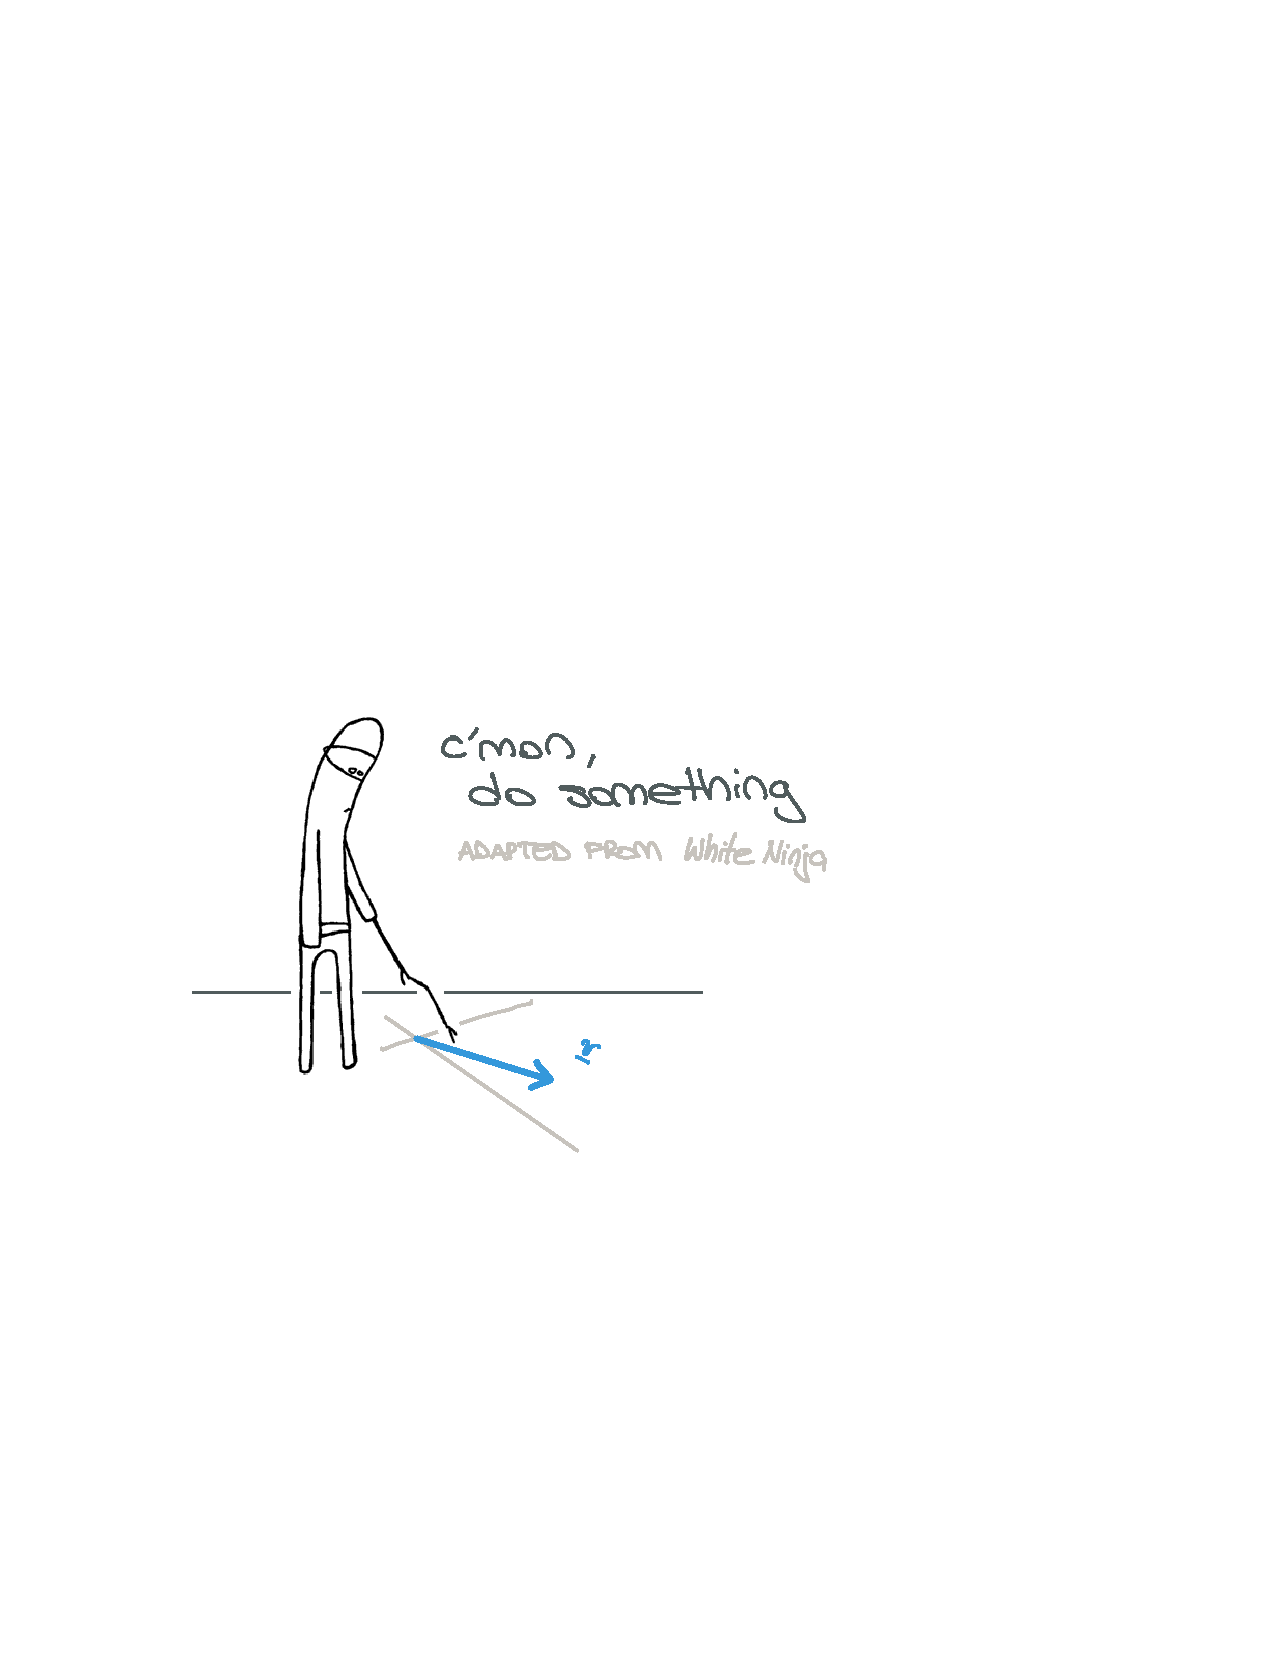
\includegraphics[width=.5\textwidth]{figures/passivetransform_dosomething.pdf}
    \caption{
        Nothing actually happens during a passive transformation. The basis vectors transform, but the components of the vector transform in such a way that $v'^i\bas{e}'_i = v^i\bas{e}_i$. Such a `transformation' may come off as uninspiring, but this is the basis of symmetries in physics. 
        From \url{https://knowyourmeme.com/memes/cmon-do-something}.
    }
    \label{fig:do:something}
\end{figure}

In a passive transformation, the vector is the same but its \emph{components} are changed because the rotated observer has different basis vectors. That is, to perform a passive transformation we \emph{rotate on the basis vectors} $\bas{e}_i \to \bas{e}'_i$ and determine what the new components $(v')^i$ must be so that
\begin{align}
    \vec{v} = v^i\bas{e}_i = (v')^i\bas{e}'_i \ .
\end{align}
One way to determine this is to act on the basis vector with the identity matrix written as $\one = R R\inv$. We choose to do this in a way that acts on the basis vector:
\begin{align}
    \vec{v} = v^{i} \bas{e}_j R\aij{j}{k}(R\inv)\aij{k}{i}  = \left[(R\inv)\aij{k}{i}v^i \right]\left[\bas{e}_j R\aij{j}{k}\right] \ .
    \label{eq:passive:rotation:1}
\end{align}
On the right hand side we recognize that the second bracketed term is simply the rotation of an object with a lower index---remember \bigidearef~\ref{idea:lower:index:rotates:with:Rinv}? Yes, all this time we had brought it up, but the basis vector $\bas{e}_i$ has a lower index, and so it transforms like a lower-indexed object (row vector-like).\footnote{To be clear, the basis vector is \emph{not} a row vector. That's why $\bas{e}_i$ is boldfaced: it carries all the abstract identity of the vector space. The basis vector just \emph{happens} to have an index that tells you how it should transform under a rotation. That index happens to be lower.} We thus define the rotated basis vectors:
\begin{align}
    \bas{e}_k' = \bas{e}_j R\aij{j}{k} \ .
\end{align}
Then \eqref{eq:passive:rotation:1} tells us that we have a linear combination of these rotated basis vectors:
\begin{align}
    \vec{v} &= 
    (v')^k
    \bas{e}_k'
    =
     (R\inv)\aij{k}{i}v^i \, \bas{e}'_k
     &
     (v')^k
     &=
     (R\inv)\aij{k}{i}v^i \ .
\end{align}
We recognize that we have rotated the basis vectors by a `forward' rotation $R$, and so the \emph{components} of a vector rotate in the opposite direction by the `backward' rotation, $R\inv$.  This is in contrast to an \emph{active} rotation of $\vec{v}$ where the basis stays the same, but we rotate the components of the vector by the forward rotation:
\begin{align}
    v^i \to (v')^i = 
    \begin{cases}
    R\aij{i}{j} v^j & \text{for an active transformation} \\
    (R\inv)\aij{i}{j} v^j & \text{for a passive transformation}
    \end{cases} \ .
\end{align}
Passive transformations are useful when we consider symmetries of systems. Each (continuous) symmetry has some analog of a `rotation' matrix, even if the rotation is not necessarily in ordinary space, but in some more abstract space. 






\section{Tensors as (Multi-)Linear Maps: Tensors}

We have informally introduced the idea that a tensor is an object with well defined transformation properties under rotations. A second perspective of tensors is that they are linear maps. This gives a slightly more rigorous definition for what all these indexed objects do. The general theme is that as linear maps, \emph{tensors are born for index contraction}.

\subsection{Products of Vector Spaces}

First, a bit of review and notation. Recall that a \textbf{vector space}, $V$, is the maximal set of vectors formed by taking linear combinations of vectors. Given a basis, $V$ is the collection of all linear combinations of those basis vectors. Now recall our jargon from Section~\ref{sec:jargon:linear:map}: linear maps are functions that take as input any element of a space and returns as output a single element of another space.\footnote{This always reminds me of rock octoroks in \emph{The Legend of Zelda: Breath of the Wild}. If you feed little baddies rusty weapons, they will inhale them and spit out a clean weapon.} A map is linear if
\begin{align}
    f(\alpha\vec{x} + \beta\vec{y}) = \alpha f(\vec{x}) + \beta f(\vec{y}) \ .
\end{align}
We can also consider functions that take more than one input. For example, a function could take two numbers and return their sum. We say that the input of this map is part of a \emph{product space} $\RR \times \RR$. What we mean here is that $\RR$ is a vector space, and $\RR\times \RR$ is a vector space where each vector in the vector space is made up of two elements of $\RR$. Does that sound familiar? This is simply what we've been calling $\RR^2$, which we now recognize is shorthand for $\RR \times \RR$. We can then imagine functions from $\RR\times \RR$ to numbers. We indicate this with the following type of notation:
\begin{align}
f:\, \RR \times \RR \to \RR    
\end{align}
For example, $f(x,y) = \sqrt{x^2 + y^2}$ gives the distance of $(x,y)$ from the origin. This kind of function is called \textbf{multi-linear} if it is linear in each of its arguments:
\begin{align}
    f(\alpha \vec{x} + \beta \vec{z}, \vec{y}) &= \alpha f(\vec{x},\vec{y}) + \beta f(\vec{z},\vec{y})
    \\
    f(\vec{x}, \gamma \vec{y} + \delta \vec{w}) &= \gamma f(\vec{x},\vec{y}) + \delta f(\vec{x},\vec{w}) \ .
\end{align}
\begin{example}
The function $f(x,y) = \sqrt{x^2 + y^2}$ is \emph{not} multi-linear. The function $g(x,y) = x+3y$ \emph{is} multi-linear.
\end{example}
\begin{example}
Is the function $f(x,y) = 2x + 5y + 2$ multi-linear?
\end{example}

The moral of this sub-section is that you should not be intimidated by the \textbf{tensor product} notation for multiple copies of a vector space, $V\times V\times \cdots \times V = V^n$. 


\subsection{Linear Maps to Numbers: Row Vectors}
\label{eq:linear:maps:row:vectors}

Our humble row vectors are also linear transformations. The components of a row vector have lower indices, $w_i$. These lower indices are just looking for an upper index for contraction. Once we provide a row vector $\row{w}$ with an object with an upper index, $\vec{v}=v^i\bas{e}_i$, then we can form the number $\row{w}\vec{v} = w_i v^i$. This tells us that a row vector $\vec{w}$ defined by its components $w_i$ is a linear map that takes in a vector and returns a number:
\begin{align}
    \row{w}: V \to \RR \ .
\end{align}
From the rule of index contraction, we observe that this is a \emph{linear map}:
\begin{align}
    \row{w}\left(\alpha\vec{v}+\beta\vec{u}\right)
    =
    w_i\left(\alpha v^i + \beta u^i\right) 
    =
    \alpha w_iv^i + \beta w_i u^i
    = 
    \alpha\row{w}\vec{v} + \beta\row{w}\vec{u} \ .
\end{align}
We deduce that lower indices are ``born to contract'' with the upper index of a vector. Lower indices say: \emph{feed me an upper index and I will contract it; I will return a number that is linearly dependent on the upper indexed components}.

We say that these row vectors belong to a \textbf{dual vector space}, $V^*$. This $V^*$ is the space of all row vectors. An element of $V^*$, say $\row{w}$, is a linear map from $V\to \RR$. 
\begin{exercise}
Argue that $V^*$ is also a vector space. If $\row{w}$ and $\row{q}$ are row-vectors, then $\alpha\row{w} + \beta\row{q}$ is also a row vector with components 
\begin{align}
    (\alpha\row{w} + \beta\row{q})_i=\alpha w_i + \beta q_i \ .
\end{align}
\end{exercise}


\subsection{Tensors as Multi-Linear Maps}

What about objects with multiple lower indices? If your tensor has $q$ lower indices, then it can take as inputs $q$ vectors and the output will be multi-linearly dependent on those inputs. Consider a tensor with two lower indices, $g_{ij}$. This is a linear map from $V\times V \to \RR$. Once you tell me the coefficients $g_{ij}$, then I can arrange them into a machine that takes in two vectors $\vec{v}$ and $\vec{u}$ and spits out a number:
\begin{align}
    g: &V\times V \to \RR
    &
    g(\vec{v},\vec{u}) &= g_{ij}v^i u^i \ .
\end{align}
This is obviously multi-linear in its arguments.

What about an object with both lower and upper indices? We already have one example: matrices have one upper and one lower index. The lower index tells us that the matrix `eats' a vector by contracting the matrix's lower index with the vector's upper index. Once you have done that contraction, you are left with an upper index. This means that the resulting object, $M(\vec{v}) = M\vec{v}$ with components $(M\vec{v})^i = M\aij{i}{j}v^j$ is a vector. We thus repeat our earlier statement that matrices are linear maps from the vector space to itself,
\begin{align}
    M: V\to V \ .
\end{align}


What if we have a tensor with two upper indices and one lower index, say $T\aij{ij}{k}$. Like a matrix, this object has a lower index and so it is a linear function on $V$. $T$ has two upper indices, which means the output is in $V\times V$. We thus say that $T: V\to V\times V$. The components of $T\vec{v}$ are $(T\vec{v})^{ij} = T\aij{ij}{k}v^k$.

Do you see how this game works? If a tensor $T$ has $p$ upper indices and $q$ lower indices, then it is a map
\begin{align}
    T: V^q \to V^p \ ,
\end{align}
where each of the $q$ lower indices a linear vector argument for the tensor, and each of the $p$ upper indices is a vector-like output. We should be a little careful about the meaning of `vector-like' here. This is not to say that you return $p$ different vectors. Instead, you have an object that transforms under rotation with $p$ factors of the rotation matrix $R$, one for each upper index. Similarly, the each of the tensor's lower indices transforms with a factor of the inverse rotation $R^{-1}$. 

What if a tensor has only upper indices? One glib way of interpreting this is that you go from nothing to an object with upper indices. For example, let $S^{ij}$ be a generic component of a tensor with two upper indices. Then I can say that
\begin{align}
    S: \RR \to V\times V \ . \label{eq:S:two:upper:O:to:VV}
\end{align}
Here $\RR$ on the left hand side just means you can input an overall coefficient. In this sense, you input a number, say $3$, and $S$ gives you $3S^{ij}$, an object with two upper indices.


\emph{Wait a second}, you think. If $S^{ij}$ only has upper indices, I know how it can still be a linear function that outputs numbers. Instead of feeding it two vectors that each have one upper index, then why not feed it two row vectors that each have one lower index? After all, $w_i q_j S^{ij}$ is a number. We thus say that there is an equivalent way of thinking about $S$:
\begin{align}
    S: V^*\times V^* \to \RR \ . \label{eq:S:two:upper:VsVs:to:R}
\end{align}
It appears that we simply took \eqref{eq:S:two:upper:O:to:VV} and pulled the $V$'s to the left-hand side, at the cost of each of them picking up a star. The rule now appears to be that for each of a tensor's indices:
\begin{enumerate}
    \item An upper index means that the tensor either has a vector-like index as an output, or it takes in a row vector as a linear input.
    \item A lower index means that the tensor either has a row-vector-like index as an output, or it takes in a column vector as a linear input. 
\end{enumerate}
\begin{example}
Consider the tensor $T\aij{ij}{k}$. This is equivalently:
\begin{align}
    T: V\to V\times V \; ,\quad 
    \RR \to V\times V\times V^* \;,\quad 
    V^* \times V \to V \; ,\quad 
    % V^* \times V^* \to V^* \; ,\quad 
    V^* \to V^*\times V^* \ .
\end{align}
What other ways can we interpret $T$ as a multilinear map between products of $V$ and $V^*$?
\end{example}

\begin{example}
Consider the tensor $T\aij{ij}{k}$. If we interpret this as a map from $V^* \times V^* \to V^*$, then we can feed $T$ two row vectors and it outputs a row vector,
\begin{align}
    T(\row{w},\row{q})_{k} = T\aij{ij}{k}w_i q_j \ .
\end{align}
Be careful that it is implicit that $T(\row{w},\row{q})$ means $T\aij{ij}{k}w_iq_j$ and not $T\aij{ij}{k}w_jq_i$. If there is ever ambiguity, it is up to you to explain to your audience exactly what you mean by a contraction. Either of the above interpretations is a valid linear map, but in general when your inputs include two or more of the same type of object, the order matters. 
\end{example}

\begin{exercise}
In the previous example we showed that the order of arguments can be somewhat ambiguous when the arguments are of the same type. Show that the order does not matter when a tensor has \textbf{symmetric} indices, say $g_{ij} = g_{ji}$. Show that the order does matter when a tensor has \textbf{antisymmetric} indices, $h_{ij} = -h_{ji}$, but that the difference is an overall minus sign. Show that a tensor with a pair of indices of the same height may be written as the sum of a piece that is symmetric and a piece that is antisymmetric in those indices. That is, for any $A_{ij}$ show that there exist symmetric $g$ and anti-symmetric $h$ such that:
\begin{align}
    A_{ij} &= g_{ij} + h_{ij}
    &
    g_{ij} &= g_{ji} 
    &
    h_{ij} &= -h_{ji} ] .
\end{align}
Argue that it does not matter if the two indices are both upper or both lower. Nor does it matter if there are other indices around.
\end{exercise}

\begin{exercise}
Show that a tensor that is symmetric with respect to two indices of the same height, say $g_{ij} = g_{ji}$, remains symmetric under a rotation. Do the same for antisymmetric pairs of indices of the same height.
\end{exercise}

The above digression of symmetric and antisymmetric indices may seem like an odd tangent. However, we will soon see that the ``additional mathematical ingredient'' that allows us to define an inner product (dot product) is an object with two symmetric lower indices that we call a metric. And while it is outside the scope of this course, antisymmetric indices are the foundation of what is called an \textbf{alternating linear map}. These, in turn, show up in differential geometry (general relativity) as something called differential $k$-forms that play the role of of infinitesimal volume elements.

\begin{exercise}
Let $T$ be a tensor with $p$ upper indices and $q$ lower indices. If I feed this tensor $p$ vectors and $q$ row vectors by contracting the indices, the result is a number. How does this number transform under rotations?
\end{exercise}


\subsection{Duality}

The above discussion should lead you to realize that there is a Yin--Yang-like duality between upper and lower indices. Initially, we started this whole course by making a big deal about \emph{vectors} and not row vectors. We had presented the \emph{nouns} of linear algebra are described by components that have one upper index. Then we presented row vectors as linear maps from $V\to \RR$, that is, row vectors are \emph{verbs} that describe an action on the \emph{nouns}. Then we realized that inasmuch as the lower index in $w_i$ is an invitation to contract with the upper index of $v^i$, we could have said it in the other way. There is a vector space $V^*$ whose components have a lower index. In this picture, the row vectors are the \emph{nouns} and the column vectors are the \emph{verbs} that represent linear maps $V^*\to \RR$. The upper index in $v^i$ is an invitation to contract with the lower index of $w_i$.

The point, of course, is that one upper index and one lower index can contract. It doesn't matter which one you call the noun and which one you call the verb (linear map). They are each the noun of their own vector space, and relative to their vector space the other vector space is a `dual space' of linear functions to $\RR$.

Generalizing this, tensors $T$ with $p$ upper indices and $q$ lower indices are multi-linear maps \emph{and} objects in themselves. If you want a tensor with $(p-1)$ upper indices and $(q-1)$ lower indices,  you could feed $T$ one row vector and one column vector. Or you could feed it a matrix, which conveniently already has an upper and a lower index. Or you could just have one of the $p$ upper indices contract with one of the $q$ lower indices, taking a multi-linear version of the trace. Or, perhaps more perversely, you could feed it a tensor with $p' < p$ upper indices and $q' < q$ lower indices in such a way that \emph{several} indices between the two tensors contract but you are left with a tensor with $(p-1)$ upper indices and $(q-1)$ lower indices. 

\subsection{A basis for the dual vector space}

The above semi-philosophical sub-section was all to motivate the following. If $V^*$ is a legitimate vector space in its own right, \emph{what are its basis vectors}? Like $V=\RR^3$, there are an infinite number of choices. But there is one ``obvious'' choice:
\begin{align}
    \rbas{e}^1 &= 
    \begin{pmatrix}
         1 & 0 & 0
     \end{pmatrix}
     &
    \rbas{e}^2 &= 
    \begin{pmatrix}
         0 & 1 & 0
     \end{pmatrix}
     &
     \rbas{e}^3 &= 
    \begin{pmatrix}
         0 & 0 & 1
     \end{pmatrix} \ .
\end{align}
The generalization to arbitrary dimensions is also obvious. Note that the basis row vectors have upper indices unlike the basis column vectors that have lower indices. This is so that a row vector is the contraction:
\begin{align}
    \row{w} = w_i \rbas{e}^i \ .
\end{align}
\begin{exercise}
How do the components $w_i$ transform under a \emph{passive transformation} where the basis row vectors are rotated by a rotation matrix $R$?
\end{exercise}


These basis row vectors are each linear maps from $V\to \RR$. For example, $\rbas{e}^2$ takes in a vector with components $v^i$ and outputs $v^2$. These basis row vectors are linear functions as far as vectors in $V$ are concerned, but they are \emph{simultaneously} a vector space in their own right. To these vectors in $V^*$, the elements of $V$ are the linear functions. 

As we have echoed several times now, the basis vectors carry the ``vector-ness'' of the objects. Thus the linear-function-ness of the $V^*$ basis can be seen in its action on the $V$ basis vectors:
\begin{align}
    \rbas{e}^i\left(\bas{e}_j\right) &\equiv \delta^i_j
    &
    \bas{e}_j\left(\rbas{e}^i\right) &\equiv\delta^i_j \ .
    \label{eq:basis:vec:row:eating}
\end{align}
On the right-hand side we have also shown that the basis vectors in $V$ are linear maps on the basis row vectors in $V^*$. When we're lazy and there is no danger of ambiguity, we drop the parenthesis and just write $\row{e}^i\vec{e}_j=\vec{e}_j\row{e}^i$.

In this way, we can ``derive'' the rule for how a row vector acts on a column vector (or equivalently vice versa):
\begin{align}
    \row{w}\vec{v} = w_i\rbas{e}^i \, v^j\bas{e}_j = w_i v^j \rbas{e}^i\bas{e}_j 
    = w_i v^j \delta^i_j
    = w_i v^i  \ .
\end{align}


\subsection{A basis for multi-linear maps}

What is the basis of tensors? Let us start with matrices. Matrix components have one upper and one lower index. They are kind of like a column vector attached to a row vector, but \emph{not acting on one another}.\footnote{Reminiscent of \url{https://en.wikipedia.org/wiki/PPAP_(Pen-Pineapple-Apple-Pen)}.} To indicate that the two basis vectors are not acting on one another, we separate them with a \textbf{tensor product} symbol, $\otimes$. Thus we expand a matrix in the basis of tensor products:
\begin{align}
    M = M\aij{i}{j} \, (\bas{e}_i\otimes \row{e}^j) \ .
    \label{eq:matrix:basis}
\end{align}
Let us see how this acts on a vector in order to ``derive'' the matrix-acting-on-a-vector rule that earlier we had simply stated as fact:
\begin{align}
    M\vec{v} =  M\aij{i}{j} \, (\bas{e}_i\otimes \rbas{e}^j) \; v^k \bas{e}_k
    = M\aij{i}{j}v^k \; (\bas{e}_i\otimes \rbas{e}^j) \bas{e}_k \ .
\end{align}
In the last line, we understand that $\rbas{e}^j$ acts on $\bas{e}_k$ (or equivalently, $\bas{e}_k$ acts on $\rbas{e}^j$). We recall that $\rbas{e}^j\bas{e}_k=\delta^j_k$. Thus:
\begin{align}
    M\vec{v} &= M\aij{i}{j}v^k \delta^j_k \, \bas{e}_i = M\aij{i}{j} v^j \bas{e}_i \ .
\end{align}
We can read the right hand side as a vector---since it is a linear combination of basis vectors $\bas{e}_i$---with components $M\aij{i}{j}v^j$, which is of course the rule that we had simply posted earlier.

From this we generalize to say that a multilinear map with $p$ upper indices and $q$ lower indices has a basis:
\begin{align}
    \bas{e}_{i_1}\otimes \bas{e}_{i_2} \otimes \cdots \otimes \bas{e}_{i_p}
    \otimes 
    \rbas{e}^{j_1}\otimes \rbas{e}^{j_2} \otimes \cdots \otimes \rbas{e}^{j_q} \ .
    \label{eq:bunch:of:basis:vectors}
\end{align}
When acting on another tensor, we simply have to specify which of the $\bas{e}_i$ and $\rbas{e}^j$ are acting on their corresponding (row-)vector components in the basis of the other tensor. 
\begin{example}
Taking a trace amounts to selecting one of the $\bas{e}_i$ and one of the $\rbas{e}^j$ in the basis to contract with each other. 
\end{example}








\section{Ket Notation}

% Basis of vectors, row vectors, etc. 

Does looking at basis elements like \eqref{eq:bunch:of:basis:vectors} give you a headache? The notation is partially to blame. s
Quantum mechanics has a completely different notation for vectors. Rather than $\vec{v}$, we write $\ket{v}$. This is called a \textbf{ket}. The reason for this is that we write row vectors as $\row{w} = \bra{w}$. We call this object a \textbf{bra}. Then the ``matrix multiplication'' $\row{w}\vec{v}$ from \eqref{eq:row:w:on:vec:v} is succinctly written $\langle w|v\rangle$. The pun is that this is a `bra--ket' or a \emph{bracket}. At the moment we do not have much use for bra and ket notation, but it is useful to establish this notation early on. It will soon be \emph{very} convenient. To summarize:
\begin{align}
    \text{column vector:}\quad \vec{v} &= \ket{v}
    &
    \text{row vector:}\quad \row{w} &= \bra{w}
\end{align}
There is no special notation for matrices, $M$. If you really want to be fancy, though, you can give matrices a hat and write them $\hat M$. This is really only important if you need to distinguish between a matrix and a number that happens to have a similar variable name. 

\begin{example}
As an example where the `hat' notation comes in handy, recall the Schr\"odinger equation in \eqref{eq:three:equations}:
\begin{align}
    \hat H \ket{\Psi} = E \ket{\Psi} \ .
\end{align}
The $\hat H$ has a hat because it is a matrix. The $E$ does not have a hat because it is a number. Does this information give the equation more significance? Obviously $\hat H \neq E$ since these are two completely different classes of objects. The equation is an equality between two vectors, $\ket{\Psi}$. Evidently, when the matrix $\hat H$ hits $\ket{\Psi}$, you end up with a new vector that is simply a rescaling of $\ket{\Psi}$. We say that $\ket{\Psi}$ is an \emph{eigenvector} of $\hat H$. 
\end{example}



\begin{table}
    \renewcommand{\arraystretch}{1.3} % spacing between rows
    \centering
    \begin{tabular}{ @{} llllll @{} } \toprule % @{} removes space
        Notation
        & $V$ element
        & $V^*$ element
        & Contraction
        & Matrix
        & Identity
        \\ \hline
        Classic
            & vector
            & row-vector
            & 
            &       
        \\
            & $\vec{v} = v^i \bas{e}_i$
            & $\row{w} = w_i \rbas{e}^i$
            & $\rbas{e}^i\bas{e}_j = \delta^i_j$
            & $M=M\aij{i}{j} \bas{e}_i\otimes \rbas{e}^j$
            & $\one$
        \\ \hline
        Quantum 
            & ket
            & bra
            &       
            &
        \\
            & $\ket{v} = v^i\ket{i}$
            & $\bra{w} = w_i \bra{i}$
            & $\langle i | j\rangle = \delta^i_j$
            & $M=M\aij{i}{j} \ket{i}\bra{j}$
            & $\ket{i}\bra{i}$
        \\ \bottomrule
    \end{tabular}
    \caption{
        Dictionary between `classic' notation and `quantum' (bra--ket) notation.
        \label{tab:classic:bra:ket:dictionary}
    }
\end{table}

Table~\ref{tab:classic:bra:ket:dictionary} provides a brief dictionary between the quantum bra--ket notation and the `classical' notation that we had been using until this point. New notation can be intimidating\footnote{More than once in my young scientific life I had discarded a textbook because it used notation that I found unintuitive. One of my mentors gently scolded me that good science and good scientists are notation-independent.}, but sometimes different notation can simplify our expressions and, in so doing, clarify ideas.\footnote{Feynman diagrams, one of the most recognizable visualizations in physics, are essentially new notation for otherwise cumbersome mathematical expressions.} 

\begin{bigidea}
Bra--ket notation is nothing more than dressing up the \emph{same} ideas above in different symbols and words. Every time you see the word \emph{ket}, your brain should immediately connect it to \emph{vector}. Every time you see a $\bra{w}$, your brain should activate the same neurons as when you see $\row{w}$. Do not let the novelty of the notation fool you into thinking there is something new going on. You already \emph{know} everything in this section, you are just learning new ways to write it.
\end{bigidea}

\subsection{Basis Bras and Kets}

Kets are vectors. The basis kets are written like so:
\begin{align}
    \bas{e}_i \equiv \ket{i} \ .
\end{align}
Just like that. The index is the name of the ket. This is potentially confusing. You lose any sense that the index is a lower index. You just have to know in your heart that a basis ket has a \emph{lower} index so that it can contract with the \emph{upper index} of the components of the ket:
\begin{align}
    \ket{v} = v^i \ket{i} \ .
\end{align}
Similarly, the basis bras have their index as their name. You have to know that the index of the basis bra is implicitly upper:
\begin{align}
    \rbas{e}^j & \equiv \bra{j}
    &
    \bra{w} &= w_j \bra{j} \ .
\end{align}

\subsection{Action of bras on kets}

The action of a bra on a ket is---by definition---the same as the action of a row vector on a column vector:
\begin{align}
    \langle w | v\rangle \equiv \row{w}\vec{v} = w_i v^i \ .
\end{align}
On the left hand side a bra and a ket combine to form a \emph{bracket}. That's peak physics humor in 1939.\footnote{Dirac, ``A New Notation for Quantum Mechanics,'' \emph{Mathematical Proceedings of the Cambridge Philosophical Society} \textbf{35} issue 3, pages 416–418.} What is implicit here is that the basis bra and basis kets combine into a Kronecker~$\delta$:
\begin{align}
    \langle {j}| i \rangle &= \delta^j_i \ . \label{eq:bra:ket:basis}
\end{align}
This is the analog of \eqref{eq:basis:vec:row:eating}, where we said that this operations connects the \emph{abstract} row and column vectors to an object, $\delta^j_i$, that tells us how the \emph{components} of the row and column vectors combine in a contraction. In a loose sense, this definition \emph{derives} the contraction rule for tensors.


\subsection{Matrices and Tensors}

Matrix components have one upper index and one lower index. This is a hint that their basis is some combination of a bra and a ket, as we already know from \eqref{eq:matrix:basis}. We thus write:
\begin{align}
    M = M\aij{i}{j} \ket{i}\otimes\bra{j}  = M\aij{i}{j} \ket{i}\bra{j}  \ .
    \label{eq:matrix:in:ket}
\end{align}
In the last step we realize that because of the shape of the bra and ket, there is \emph{no ambiguity} that the ``ket--bra'' $\ket{i}\bra{j}$ might be intepreted as a contraction. The contractions are only when the vertical parts of the bra and ket overlap, as in \eqref{eq:bra:ket:basis}. We can extend our notation to general tensors as long as we take the convention where the upper indices all come first and the lower indices are last:
\begin{align}
   T= T\aij{i_1\cdots i_p}{j_1\cdots j_q} \ket{i_1}\cdots\ket{i_p}\bra{j_1}\cdots\bra{j_q} \ .
\end{align}
If your tensor does not have all of the upper indices first, you can always define a new tensor which has identical components but reshuffled so that the components that are all upper index come first. When you act with one tensor onto another tensor you typically need to specify which bras and kets you intend to contract. Finally, if you are ever in doubt, you can always explicitly write the tensor product symbol $\otimes$.\footnote{Every time I do this I quietly hum the theme to the 90's \emph{X-Men} animated series.} 


\subsection{Ket Tricks}


% Test: $\ket{^i}$ $\bra{_j}$ $\left/ ^i \right\rangle \left\langle _j \right/$

% Identity

% \begin{align}
%     \left\langle ^i  \middle/ w_i A\aij{k}{\ell} v^j \middle/  _j\right\rangle
% \end{align}

The identity matrix is blindingly obvious and will turn out to be rather significant for us soon:
\begin{align}
    \one = \ket{i}\bra{i}  = \ket{1}\bra{1} + \ket{2}\bra{2} + \ket{3}\bra{3} + \cdots
\end{align}
\begin{exercise}
Remember that the ket is implicitly a lower indexed object and the bra is implicitly an upper indexed object, thus their repeated $i$ index is contracted. It is worth taking time to understand this expression in as many ways as you are able to. Instead of ket--bras, please use row vectors and column vectors in $\RR^3$. Confirm that this $\ket{i}\bra{i}$ acting on a three-vector gives the same three vector. What would happen if you dropped the last term and instead only wrote $\ket{1}\bra{1} + \ket{2}\bra{2}$? What is the effect of this not-quite identity matrix on a three-vector $\vec{v}=\ket{v}$ with components $v^i$?
\end{exercise}

Another surprisingly useful expression is the trace of a matrix:
\begin{align}
    \Tr M = \langle i | M | i \rangle \ .
    \label{eq:trace:in:ket}
\end{align}
Here we recognize again that the upper index of the bra is contracting with the lower index of the ket. 
\begin{exercise}
Confirm \eqref{eq:trace:in:ket} by inserting \eqref{eq:matrix:in:ket} for $M$. 
\end{exercise}







\section{Metric Spaces: Dot Products}
\label{sec:metric:spaces}

A vector space $V$ is a collection of abstract objects (vectors, kets) and their linear combinations. We defined related spaces based on the linear transformations on the vector space. This includes row vectors (bras) which live in a dual vector space $V^*$, and all tensor products of these spaces. We saw that matrices---and tensors in general---can be understood as linear transformations between these spaces. 

Now we turn the idea of a \textbf{dot product}, which we introduced for Euclidean three-space in \eqref{eq:euclidean:3d:metric:intro}.  The dot product took in two vectors and returned a number. This means that it is a multi-linear map from $V\times V \to \RR$. The generalization of the dot product is called the \textbf{inner product} and the tensor associated with it is called the \textbf{metric}. We write the inner product with a bracket notation that looks (intentionally) similar to a ket acting on a bra:
\begin{align}
    \langle \, \cdot \, , \, \cdot \, \rangle  = g_{ij} \; : V\times V \to \RR \ .
\end{align}
The nomenclature of using $g_{ij}$ for the metric is inherited from relativity. The nomenclature with the bracket notation is inherited from quantum mechanics. There is one other defining characteristic of the metric: it is \emph{symmetric} in its indices:
\begin{align}
    g_{ij} = g_{ji} \ .
\end{align}
The metric is a special tensor that we have to specify. A vector space with a metric is called a \textbf{metric space} or and \textbf{inner product space}. $\RR^3$ is a vector space. $\RR^3$ with a metric---say, the Euclidean metric in \eqref{eq:euclidean:3d:metric:intro}---is a metric space. 
\begin{bigidea}
The difference between a vector space and a metric space is that in a metric space, you can raise/lower indices (transpose or \emph{Hermitian conjugate} for spaces with complex numbers) and measure length and angles between vectors. There can be choices of metrics on the same vector space.
\end{bigidea}

The most common example is $N$-dimensional \textbf{Euclidean space}, a metric space where the components of the metric $g_{ij}$ are simply that of the $N\times N$ identity matrix:
\begin{align}
    g_{ij} &= \text{diag}(1,\cdots 1) = 
    \begin{pmatrix}
        1 & & \\
        & \ddots & \\
        & & 1
    \end{pmatrix} \ .
\end{align}
% 
\begin{bigidea} \label{idea:treating:two:index:as:matrix}
Let me be clear: $g_{ij}$ is not a ``matrix'' in the sense that acting with it on a vector does not produce a vector. $g_{ij}$ are the \emph{components} of a tensor that is a symmetric\footnote{Meaning $g_{ij}=g_{ji}$ or equivalently $g(\vec{v},\vec{w}) = g(\vec{w},\vec{v})$.} map from $V\times V\to \RR$.
% 
However, because $g_{ij}$ has two indices, we may visually arrange the components in a $N\times N$ table, where $N$ is the dimension of the vector space. If you want you can call this table a matrix, though in these notes we have taken a more strict definition. In general---but specifically in Section~\ref{sec:rotations:isometries} where this comes up---when we write something of the form
\begin{align}
    A_{ij} = 
    \begin{pmatrix}
        a & b \\
        c & d
    \end{pmatrix} \ ,
\end{align}
all we mean is that $A_{11} = a$, $A_{12} = b$, and so forth. We can then talk about index contraction as ``matrix multiplication'' as long as consecutive indices are contracted:
\begin{align}
    A_{ij}B\aij{j}{k} = (AB)_{ik} = 
    \begin{pmatrix}
        A_{11} & A_{12} \\
        A_{12} & A_{22}
    \end{pmatrix}
    \begin{pmatrix}
        B\aij{1}{1} & B\aij{1}{2} \\
        B\aij{2}{1} & B\aij{2}{2}
    \end{pmatrix} \ .
\end{align}
If consecutive indices are not contracted, then you need to arrange things a bit more carefully. Specifically:
\begin{align}
    A\aij{k}{i} B_{k\ell} C\aij{\ell}{j} \neq 
     \begin{pmatrix}
        A\aij{1}{1} & A\aij{1}{2} \\
        A\aij{2}{1} & A\aij{2}{2}
    \end{pmatrix} 
    \begin{pmatrix}
        B_{11} & B_{12} \\
        B_{12} & B_{22}
    \end{pmatrix}
    \begin{pmatrix}
        B\aij{1}{1} & B\aij{1}{2} \\
        B\aij{2}{1} & B\aij{2}{2}
    \end{pmatrix} \ .
\end{align}
But if we define\footnote{The transpose swaps the order of the indices of a matrix. What about the height of the indices? For now let us maintain the height so that an the first, upper index of $A$ becomes the second, upper index of $A^T$. We give a more formal definition of transpose in Section~\ref{eq:transpose:adjoint}.} $(A^T)_i^{\phantom{i}k} = A\aij{k}{i}$, then we may write
\begin{align}
    A\aij{k}{i} B_{k\ell} C\aij{\ell}{j} =
    (A^T)_i^{\phantom{i}k} B_{k\ell} C\aij{\ell}{j}&=
     \begin{pmatrix}
        A\aij{1}{1} &  A\aij{2}{1} \\
        A\aij{1}{2} & A\aij{2}{2}
    \end{pmatrix} 
    \begin{pmatrix}
        B_{11} & B_{12} \\
        B_{12} & B_{22}
    \end{pmatrix}
    \begin{pmatrix}
        B\aij{1}{1} & B\aij{1}{2} \\
        B\aij{2}{1} & B\aij{2}{2}
    \end{pmatrix} 
    \\ &=
    \begin{pmatrix}
        (ABC)^{11} & (ABC)^{12} \\
        (ABC)^{12} & (ABC)^{22}
    \end{pmatrix}
    \label{eq:ABC:matrix:multiplication:tensor:note}
    \ .
\end{align}
% 
This is a modest point that can cause some confusion later on. 
\end{bigidea} %% \label{idea:treating:two:index:as:matrix}



Metrics do two things for us:
\begin{enumerate}
    \item They allow us to define the length of a vector, $|\vec{v}|$. In so doing, they allow us to define a unit length (\emph{normalized}) vector, $\hat{\vec{v}}$.
    \item They allow us to define the angle between two vectors, $\cos\theta = \langle v,w\rangle$.
\end{enumerate}
Together, they allow us to define \emph{nice} basis vectors that are unit length and orthogonal to one another. We say that such a basis is \textbf{orthonormal}.


\subsection{Example Polar Coordinates}

The Euclidean space metric is too boring. It is essentially the identity element and it seems like there's much ado about nothing. Let me motivate the idea of a metric by reviewing polar coordinates. This is the simplest form of what are called \textbf{curvilinear coordinates}. These are simply coordinates grids that are not straight lines, the way that the Cartesian $x$--$y$ plane is a grid. Polar coordinates replace $(x,y)$ with $(r,\theta)$. Here $r$ is the distance from the origin and $\theta$ is the angle from the positive $x$-axis. 
% 
This example is surprisingly subtle. The take-away is that the metric in polar coordinates is
\begin{align}
    g_{ij} = 
    \begin{pmatrix}
        g_{rr} & g_{r\theta} \\
        g_{\theta r} & g_{\theta\theta}    
    \end{pmatrix}
    =
    \begin{pmatrix}
        1 & \\
        & r^2
    \end{pmatrix} \ .
    \label{eq:polar:metric}
\end{align}
The bottom right component is not one, but rather the radial coordinate. If this is your first time seeing this, please feel free to \emph{skim} this section. We will present the example, then dig a bit deeper to discuss the significance. You may want to postpone reading those details until after reviewing these notes once through.

\subsubsection{What does this mean}

The surprising piece in \eqref{eq:polar:metric} is that $g_{\theta\theta} = r^2$. This means that the metric changes as you move further away from the origin of the coordinate space. This is in contrast to the Euclidean metric whose components are proportional to the identity no matter where you happen to be.

This should not surprise us. We know that the same \emph{angular displacement} $\Delta \theta$ corresponds to a different traversed circumference depending on the radius. If you are close to the origin, then a displacement of $\Delta\theta$ is not particularly far. If you are far from the origin, then a displacement of $\Delta\Theta$ can be huge, see Fig.~\ref{fig:polar:displacement}.\footnote{This sometimes shows up in the ``paradox'' (it is not a paradox) that ``shadows travel faster than the speed of light.''} From a physics perspective, you could have guessed this from pure dimensional analysis: $\Delta \theta$ is dimensionless. If you want your metric to output a squared distance, then you need something with dimensions of length---the only plausible candidate is $r^2$. This is illustrated nicely in the \emph{Calvin and Hobbes} comic in Fig.~\ref{fig:CH:record:player}.



\begin{figure}[tb]
    \centering
    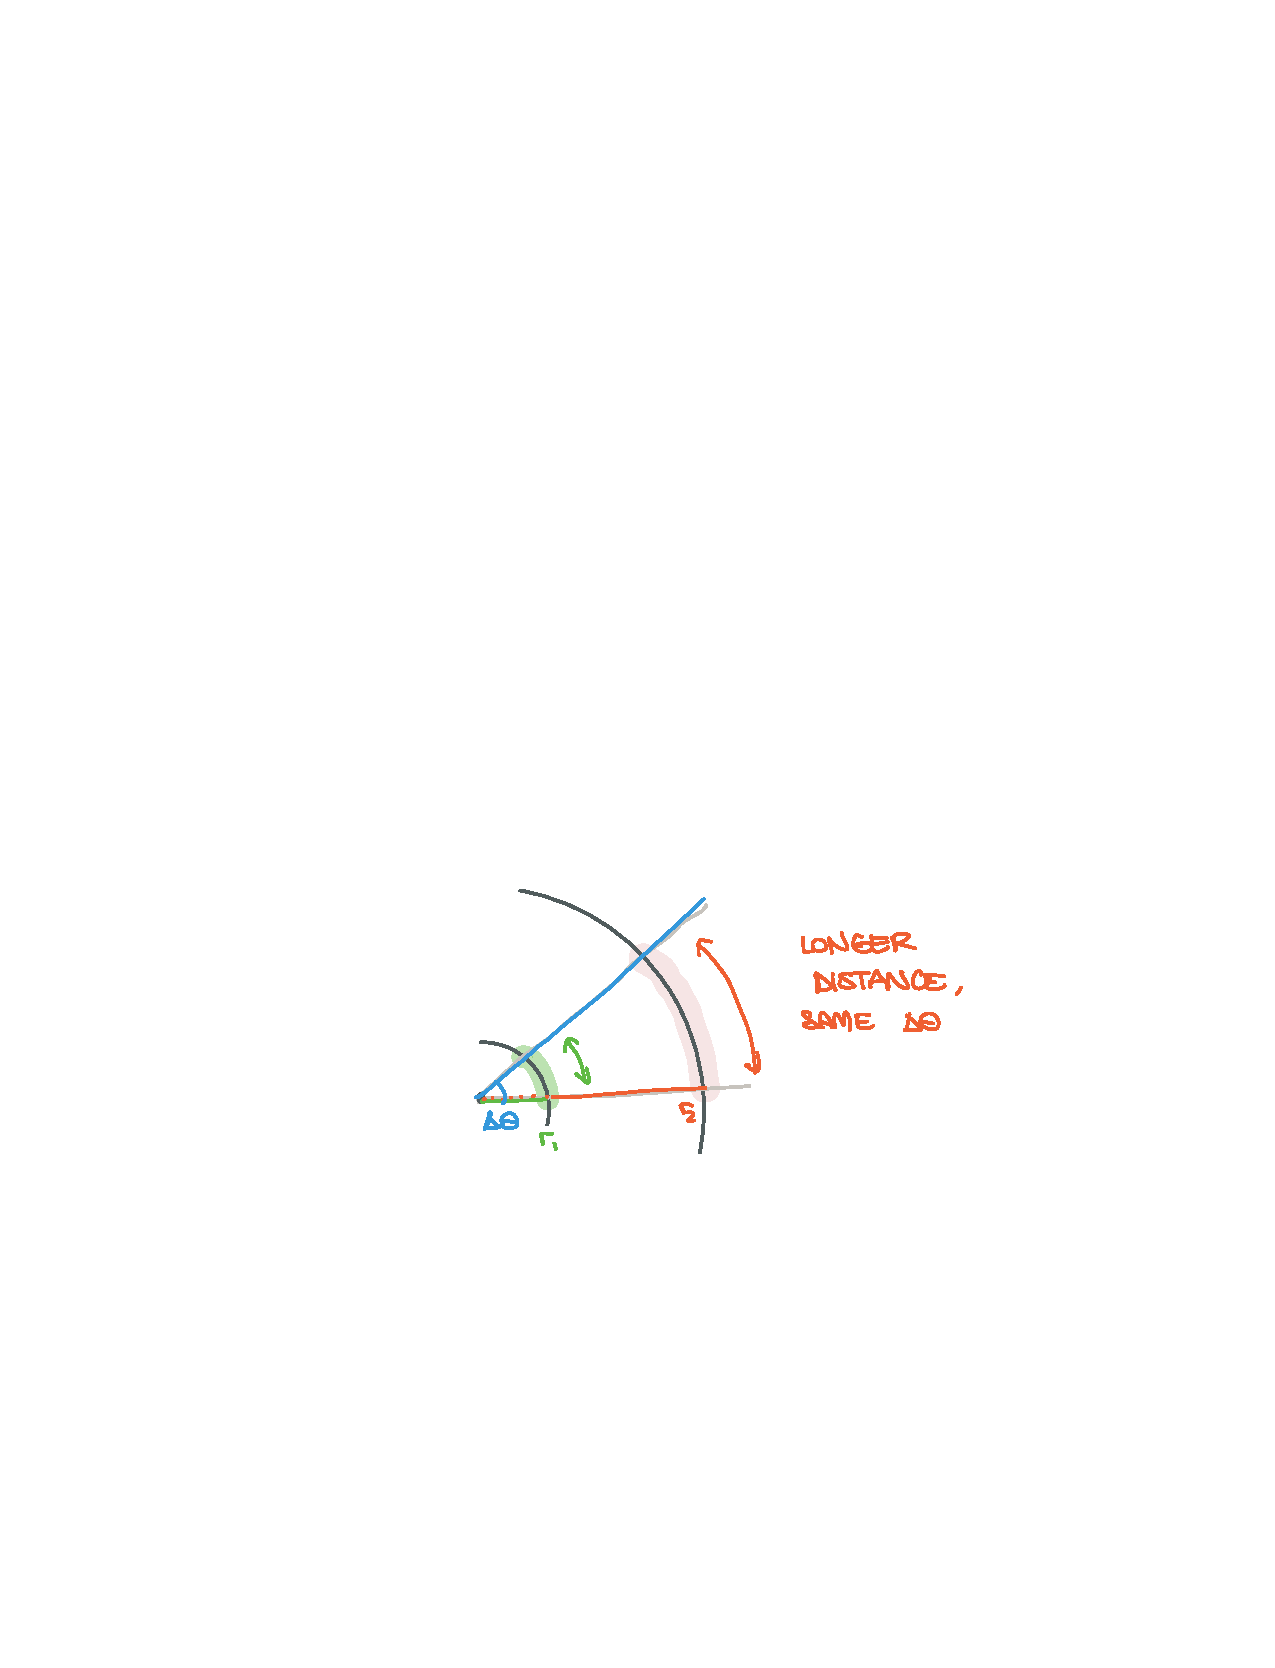
\includegraphics[width=.4\textwidth]{figures/polar_longer_distance_dtheta.pdf}
    \caption{The meaning of the $g_{\theta\theta} = r^2$ is related to the idea that the distance traversed along a circle for a displacement $\Delta\theta$ depends on the radius of the circle.}
    \label{fig:polar:displacement}
\end{figure}

\begin{figure}[tb]
    \centering
    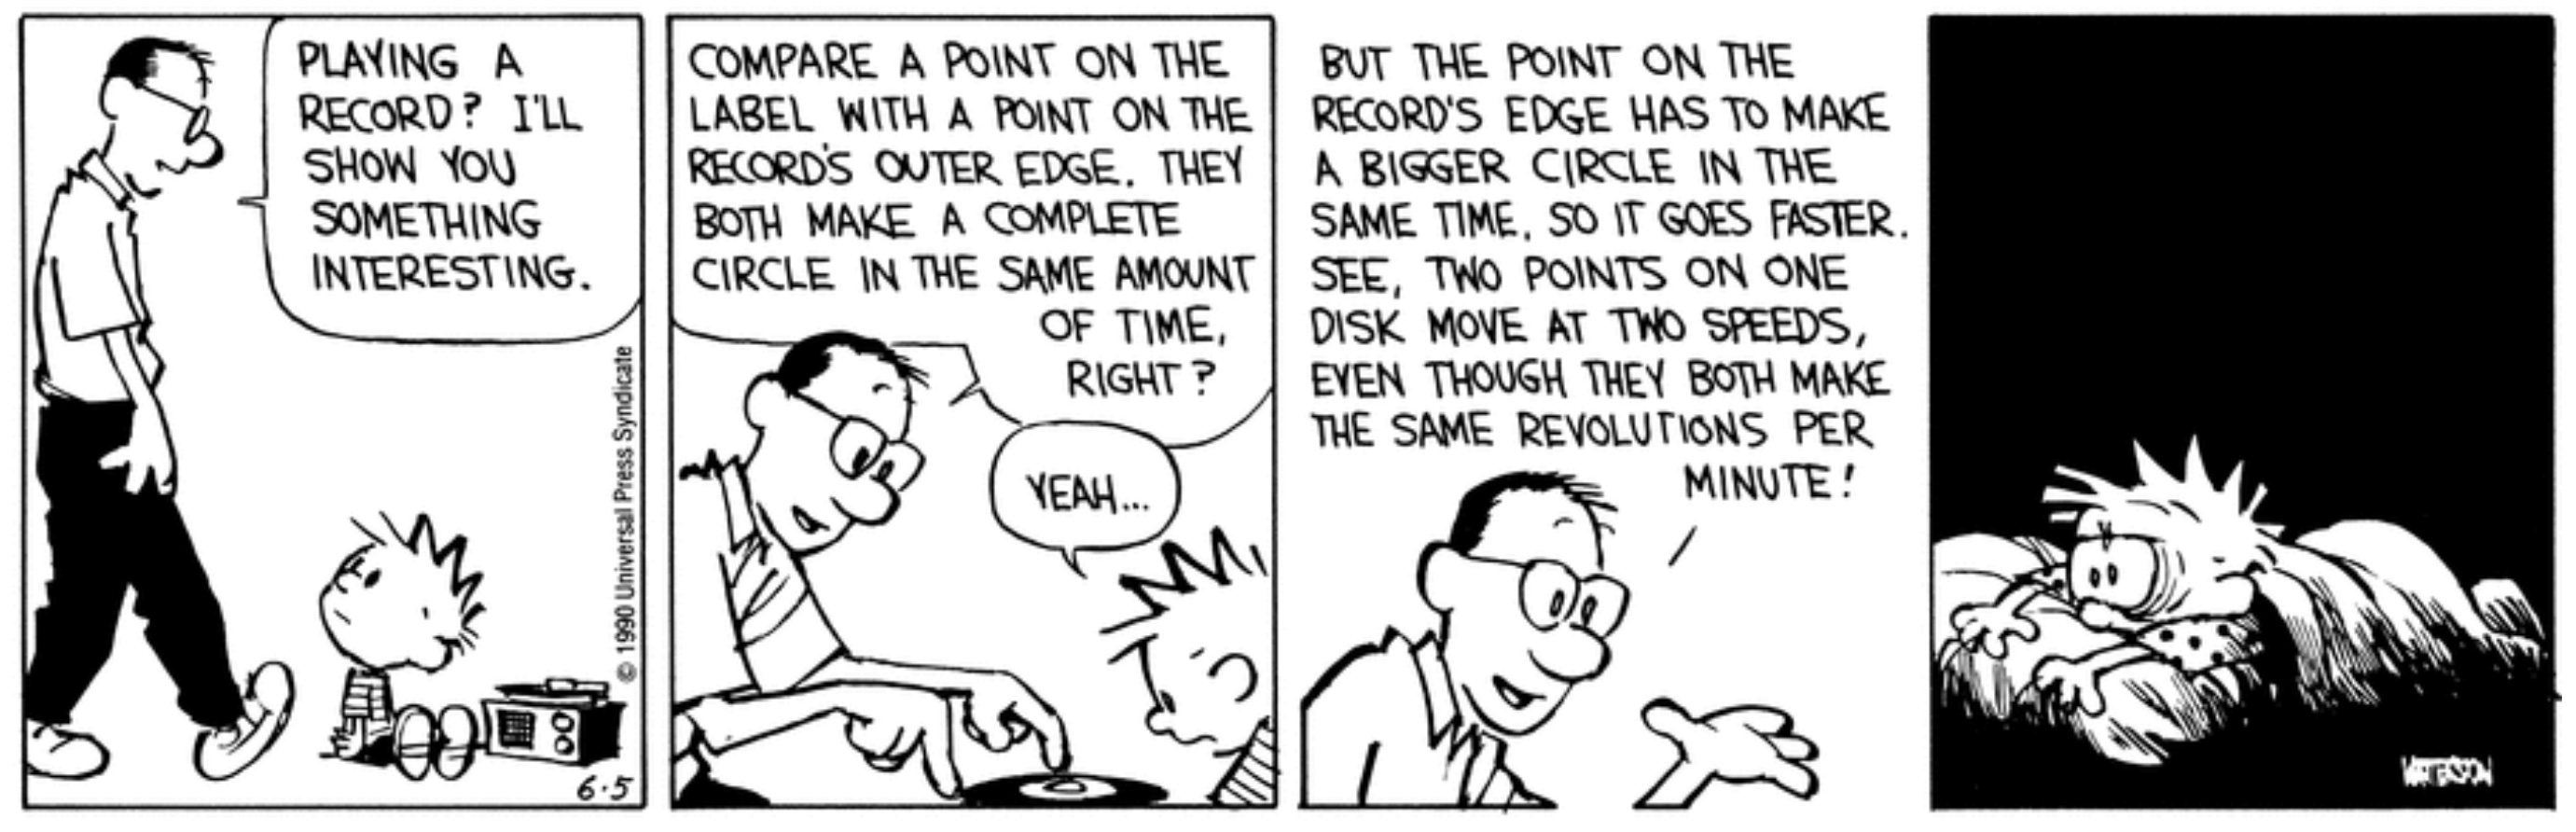
\includegraphics[width=\textwidth]{figures/calvin_and_hobbes_record.jpg}
    \caption{\emph{Calvin and Hobbes}, ``Record Player,'' by Bill Watterson, 5 June 1990. Image from \url{https://www.gocomics.com/calvinandhobbes/1990/06/05}. If you have never heard of a record player than look it up.}
    \label{fig:CH:record:player}
\end{figure}
% Also: mechanical integrator: https://www.youtube.com/watch?v=s-y_lnzWQjk
% Also: differential steering: https://www.youtube.com/watch?v=yYAw79386WI

\begin{example}
While this is not really relevant for linear algebra, there are a few neat ways in which the difference between angular and linear velocity show up. One is the mechanical integrator\footnote{\url{https://www.youtube.com/watch?v=s-y_lnzWQjk}}, and another is differential steering\footnote{\url{https://www.youtube.com/watch?v=yYAw79386WI}}. 
\end{example}


\begin{exercise}\label{ex:polar:location:dependence}
Consider the vector $\vec{v} = 3\bas{e}_r - (\pi/4)\bas{e}_\theta$ located at the point $(r,\theta)=(2, \pi/6)$. Find the length of this vector, $|\vec{v}|$ using the polar coordinate metric \eqref{eq:polar:metric}. Observe that for this problem we have to specify the location of the vector; this corresponds to defining where the `zero' of the vector space is relative to the coordinate space. This suggests that there's more structure here than simply a metric space---we discuss this in Section~\ref{sec:polar:tangent:space}.
\end{exercise}

\subsubsection{What else do we notice?}

The metric depends on the location of the vector---please make sure to do Exercise~\ref{ex:polar:location:dependence}. This is in contrast to the ordinary Euclidean metric, which is the same no matter where you are in coordinate space. Another difference is that the orientation of the polar basis vectors is different compared to the Cartesian basis vectors that always point in the $x$- and $y$-directions, see Fig.~\ref{fig:polar:coordinate:vs:vector:space}. In fact, the orientation of the polar basis vectors is different depending on where in the coordinate space you happen to be looking, see Fig.~\ref{fig:polar:coordinate:vs:vector:space:two:points}. Note that the length and orthogonality of the polar coordinate basis vectors do not change, just their relative orientation. 

\begin{figure}[tb]
    \centering
    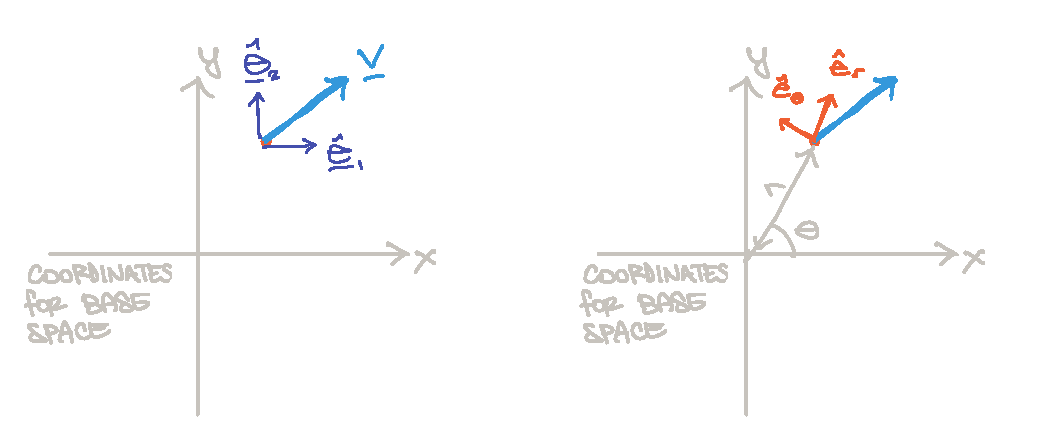
\includegraphics[width=.8\textwidth]{figures/PolarBasis.pdf}
    \caption{Consider a point in $\RR^2$ and some vector $\vec{v}$ that represents the velocity of a particle at that point. We can write $\vec{v}$ in the usual Cartesian basis (left), or in the polar basis (right). Both bases are orthonormal, but they are oriented differently.}
    \label{fig:polar:coordinate:vs:vector:space}
\end{figure}


\begin{figure}[tb]
    \centering
    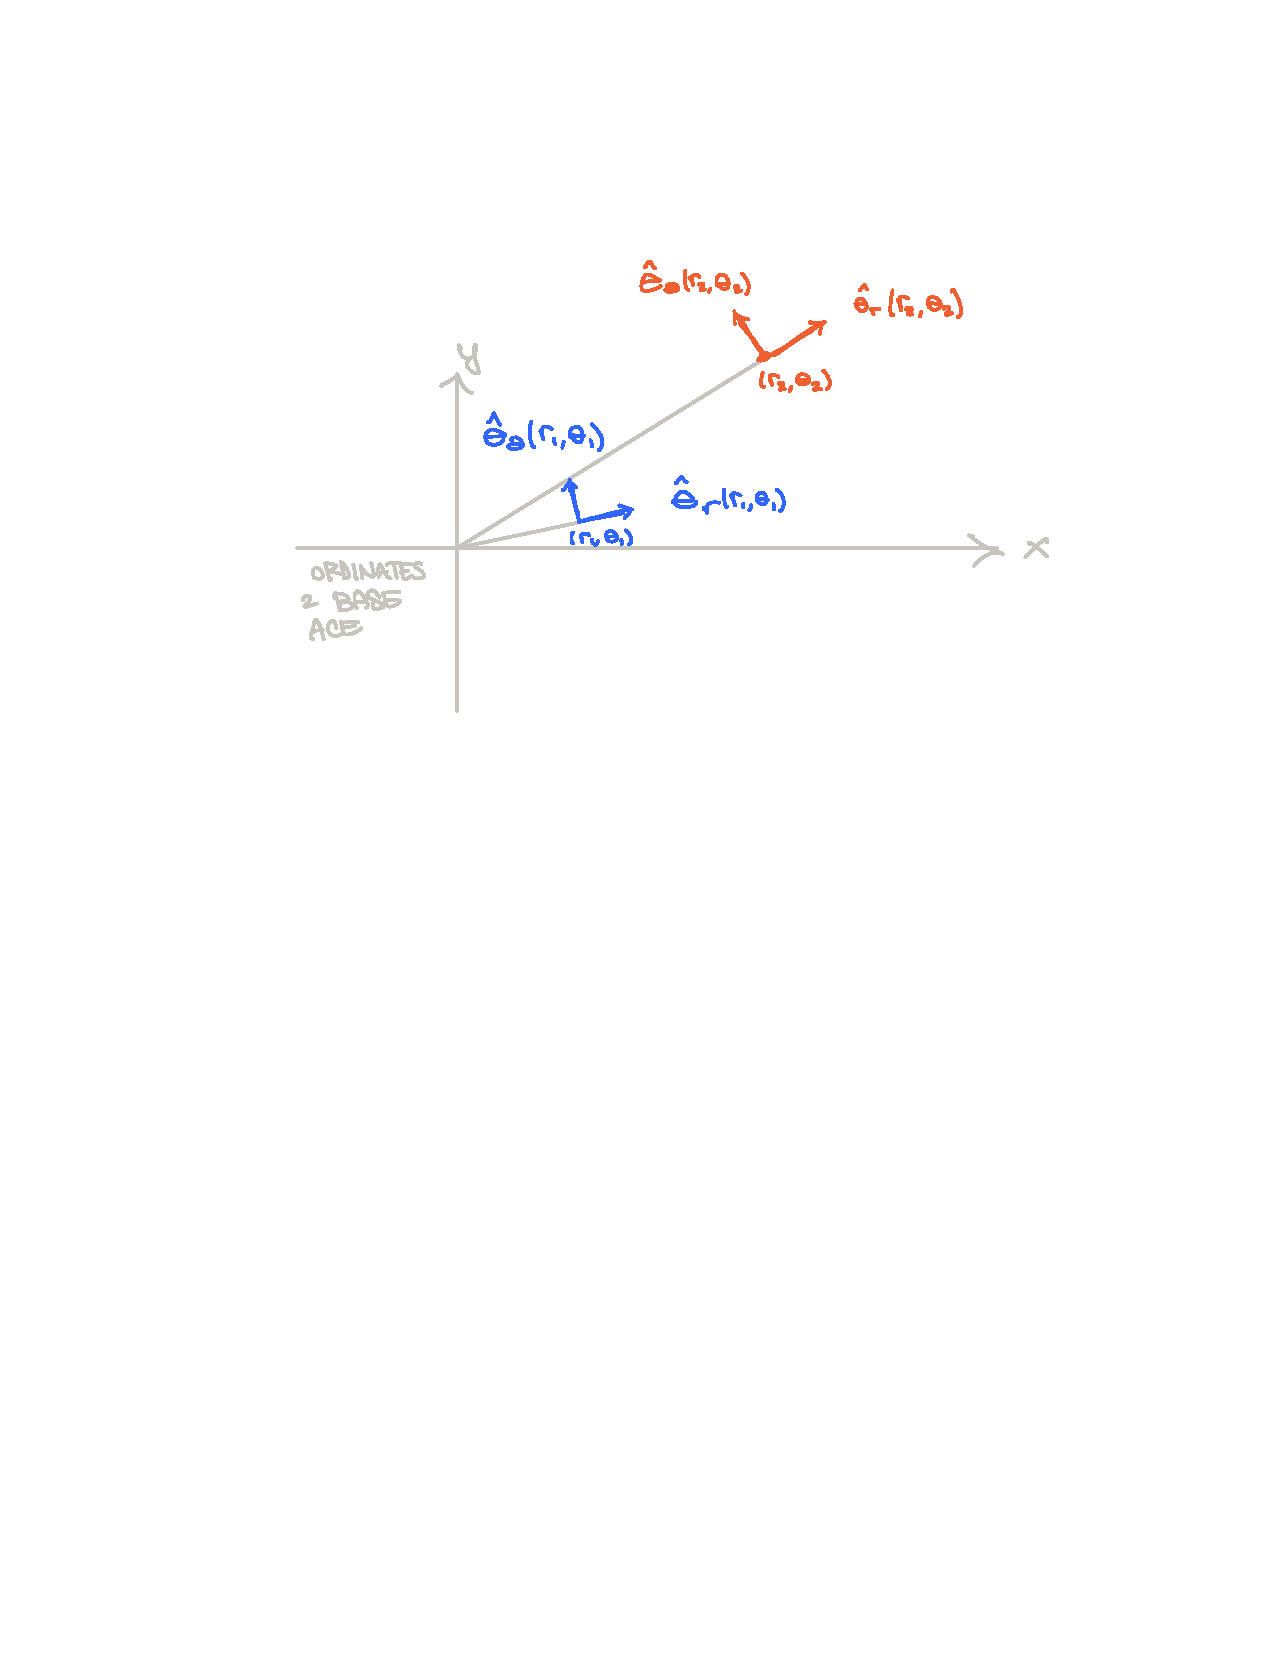
\includegraphics[width=.6\textwidth]{figures/polar_different_orientation.pdf}
    \caption{The basis vectors are a basis for potential velocities of a particle at that point. The orientation of the polar coordinate basis vectors depends on the point at which we are using them. }
    \label{fig:polar:coordinate:vs:vector:space:two:points}
\end{figure}


When a metric that differs from the identity\footnote{By which we mean a metric whose components are different from the components of the identity matrix. See \bigidearef~\ref{idea:treating:two:index:as:matrix}.} we should suspect that we may be in a \emph{curved space}. For example, the surface of the Earth is a curved space whose metric in spherical coordinates is
\begin{align}
    g_{ij} = 
    \begin{pmatrix}
        g_{\theta\theta} & g_{\theta\phi}\\
        g_{\phi\theta} & g_{\phi\phi}
    \end{pmatrix}
    =
    \begin{pmatrix}
        r^2 & \\
        & r^2 \sin^2\theta
    \end{pmatrix} \ ,
    \label{eq:metric:surface:of:sphere}
\end{align}
where $r$ is the radius of the Earth. However, it is not true that all `funny looking metrics' imply that the underlying space is curved. In the polar coordinate example of this subsection, the space itself is the same two-dimensional Euclidean space that we are used to. All we have done is changed coordinates. We see that a funny looking metric may mean that the space is curved, or it may mean that our coordinate system is curved (that is, \emph{curvilinear}). 

\begin{exercise}
Prove \eqref{eq:metric:surface:of:sphere}. You may need to review your trigonometry and draw the sphere carefully. Observe that this is a two-dimensional metric space for the surface of the sphere. There is no radial vector. Feel free to derive the three-dimensional spherical coordinate metric that includes the radial direction. 
\end{exercise}

\subsubsection{The polar basis}

Let us check the orthonormality of the polar basis at some point, $(r,\theta) = (3,\pi/4)$. The fact that $\bas{e}_r$ and $\bas{e}_\theta$ are orthogonal should be obvious: one points in the radial direction and one points in the polar direction---these are orthogonal directions by definition. Another way of seeing this is that the metric is diagonal. 
\begin{exercise}
Confirm that if a metric is diagonal, then the basis vectors are obviously orthogonal. 
\end{exercise}
The length of the $\bas{e}_r$ vector is also normalized since $\langle \bas{e}_r, \bas{e}_r\rangle = g_{rr} = 1$. What about the length of $\vec{e}_\theta$? This is a vector corresponding to a shift of one unit in the $\theta$ direction. We have
\begin{align}
    \langle \vec{e}_\theta, \vec{e}_\theta \rangle = g_{\theta\theta} = r^2 \ .
\end{align}
Well that's unusual. If we are at $r=3$, then $\langle \vec{e}_\theta, \vec{e}_\theta \rangle = 9$. This means that the normalized basis vector is
\begin{align}
    \bas{e}_\theta = \frac{\vec{e}_\theta}{r} \ .
\end{align}
This makes sense because a `shift of one unit in the $\theta$ direction' is a much larger step the further away you are from the coordinate origin, as we saw in Fig.~\ref{fig:polar:displacement}.




\subsubsection{The tangent space}
\label{sec:polar:tangent:space}

This example of polar coordinates is helpful because it is a simple case of a funny-looking metric that should feel familiar to us. However, it is also a very dangerous example because it can lead to some misconceptions. In fact, you should have noticed that something funny was going on here. The metric \eqref{eq:polar:metric} depends on the `position' of the vector---where `base' of the vector located. 

This notion of `position' should make you feel uncomfortable. Positions depend on a coordinate system. We remarked before that there is no such thing as a ``position vector'' and that ``position space'' is not a vector space---see Exercise~\ref{ex:position:vector}. Positions depend on a choice of origin, whereas in a vector space there is no `origin,' only the zero vector. The zero vector is independent of the choice of basis vectors. There is no such thing as `translating' a vector in a vector space.\footnote{You can add vectors, but one should not think about this as translation because there is a more subtle idea of how to translate a vector across a curved surface. The word `translate' is being used differently, but to avoid potential confusion there is no need to talk about vector addition within a vector space as `translation.'} What is happening here is that there is a separate space called the \textbf{base space} or \textbf{manifold}.\footnote{This comes with some mathematical assumptions about topology, but for our present purposes just assume that the manifold is something like a sheet of graph paper whose grid lines gives us a coordinate system.} We call the base space $M$, in our present example $M \simeq \RR^2$.

The base space is not a vector space. It has an origin. You can choose different coordinates that have a different origin---for example, you could shift your Cartesian coordinates to the right by one unit. You can choose curvilinear coordinates like polar coordinates. All this is to say that a given \emph{point} on the base space, $p$, has many different representations depending on your coordinate system. Let's just call it $p$, but to some people $p$ corresponds to a specific value of $(x,y)$, to others its a value of $(r,\theta)$. 

Now imagine a particle at position $p$. Maybe that particle is moving. It has a velocity. The space of possible velocity vectors \emph{is a vector space}. The vector space is called the tangent space at $p$, which math-y folks call $T_pM$. This is a special two-dimensional vector space that \emph{looks a lot like} the base space, but it is not. The velocity vectors obey the rules for a vector space: you can take linear combinations, there is a well defined zero vector, and so forth. In particular, the vectors are independent of any particular coordinate system of the base space. They have their own basis, which we can draw as a set of vectors whose base is ``at'' $p$. This is illustrated in Fig.~\ref{fig:tangent:space:polar}.  We can determine a basis for each tangent space by using the coordinates. The polar basis comes from considering the directions that infinitesimal changes in $r$ and $\theta$ correspond to at the point $p$.\footnote{Do you see how this now interfaces with multivariable calculus? The marriage of calculus and geometry is called differential geometry.}

\begin{figure}[tb]
    \centering
    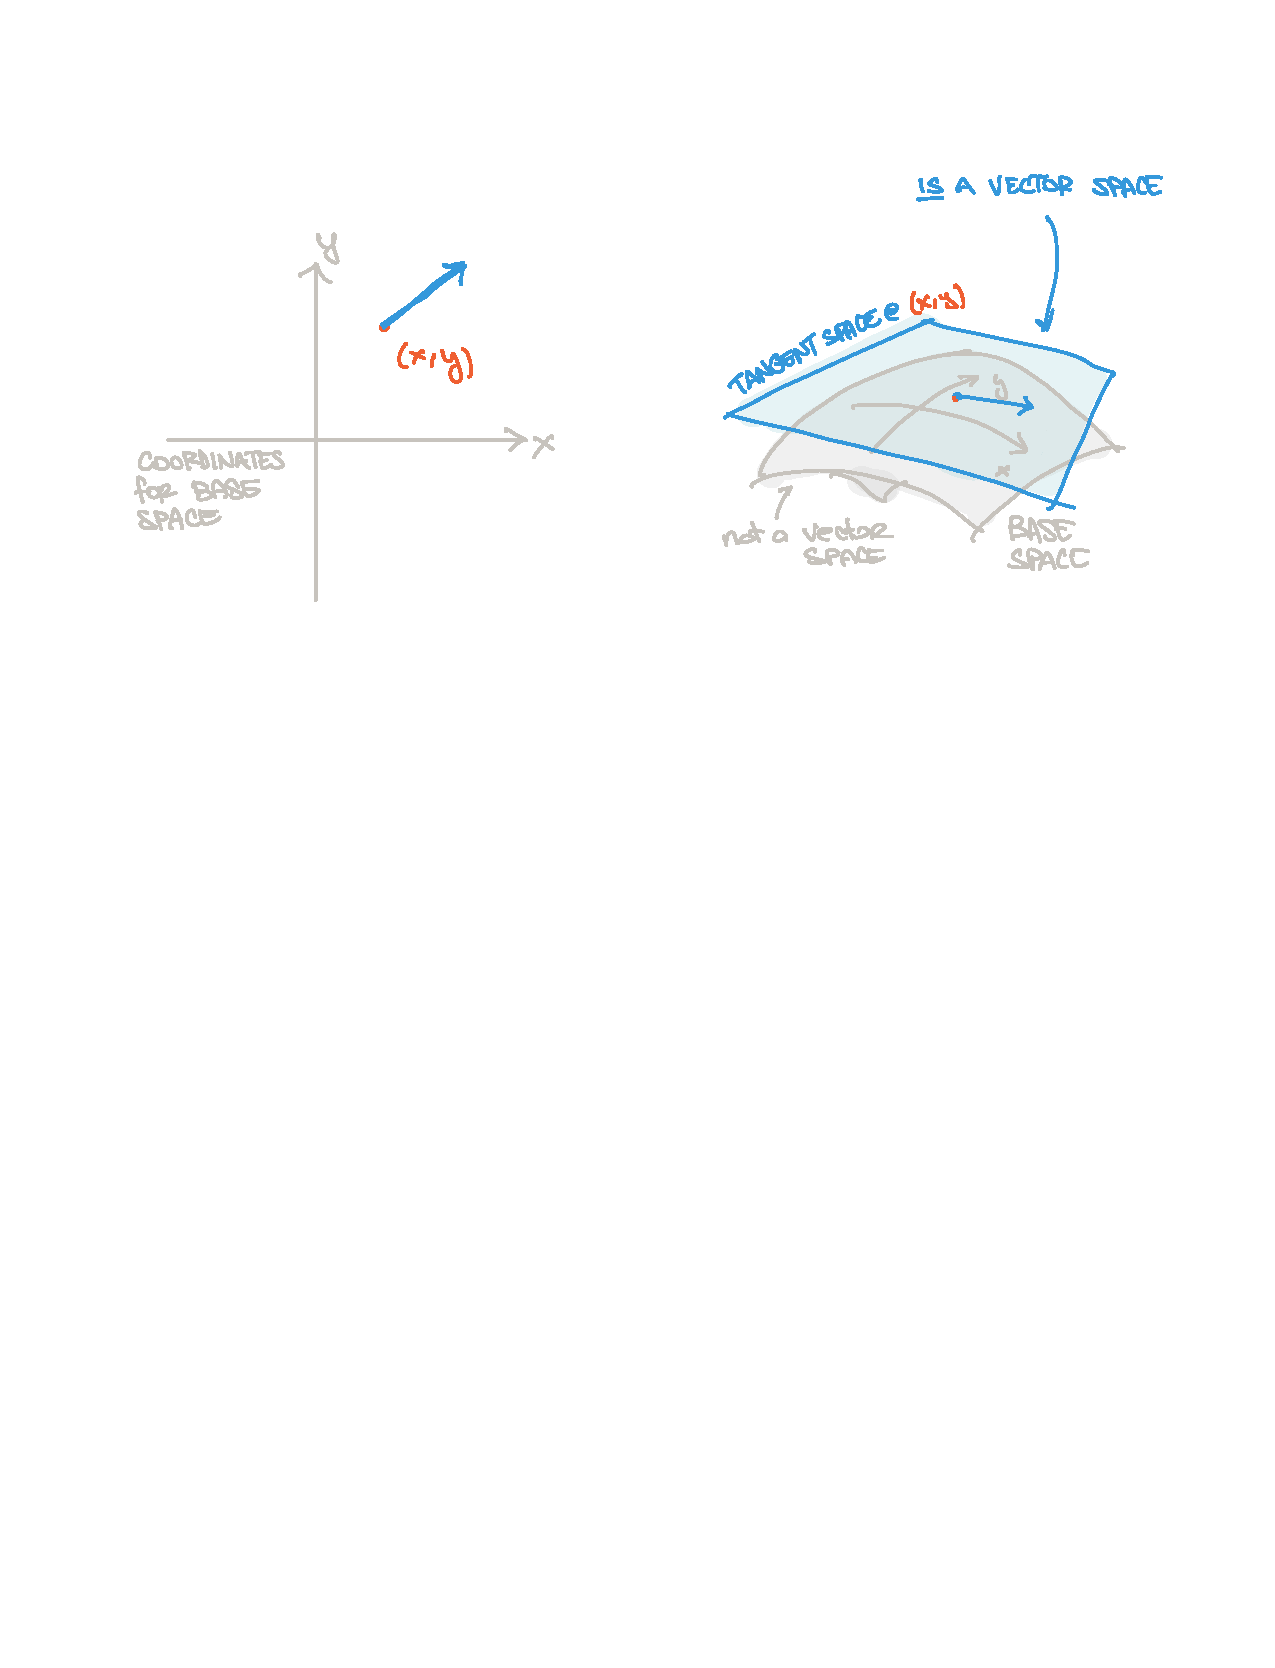
\includegraphics[width=.7\textwidth]{figures/base_space_tangent_space.pdf}
    \caption{The base space is ``coordinate space.'' These are positions. Positions are not vectors and the base space is not a vector space. Positions depend on the coordinate system. At each position $(x,y)$, there is a vector space called the tangent space at $(x,y)$. This \emph{is} a vector space and the vectors can be thought of as possible velocities of a particle at $(x,y)$. In the picture on the right hand side we have `peeled' the base space away from the tangent space to make it clear that they are different, even though they both look like sheets of paper. There is no assumed curvature in the base space. There is a different tangent space for each position. The combination of the infinite number of tangent spaces over the base space is known as a tangent space bundle.}
    \label{fig:tangent:space:polar}
\end{figure}

The metric is defined for \emph{each} tangent space. There are an infinite number of tangent spaces, one for each point $p$ in the manifold. The polar coordinate metric~\eqref{eq:polar:metric} tells us the following. Suppose you have a point $p$ with a tangent space $T_pM$. What is the appropriate metric for this space if you are using the polar basis vectors? Take \eqref{eq:polar:metric} and plug in the value of $(r,\theta)$ corresponding to $p$. In this case the metric is independent of $\theta$. Suppose you are at a point 2 units from the origin and $\pi/6$ from the $x$-axis, $(r,\theta)=(2,\pi/6)$. Then the metric for the tangent space at this point is
\begin{align}
    \left.g_{ij}\right|_p=
    \left.
    \begin{pmatrix}
        1 &\\
        & r^2
    \end{pmatrix}
    \right|_{r=2}
    =
    \begin{pmatrix}
        1 &\\
        & 4
    \end{pmatrix} \ .
\end{align}
If you are at a different point $p'$ with $r=3$, then the metric for $T_{p'}M$ is instead
\begin{align}
    \left.g_{ij}\right|_{p'}=
    \left.
    \begin{pmatrix}
        1 &\\
        & r^2
    \end{pmatrix}
    \right|_{r=3}
    =
    \begin{pmatrix}
        1 &\\
        & 9
    \end{pmatrix} \ .
\end{align}
In this way, once you specify the point $p$, you have an unambiguous metric for $T_pM$ 


\begin{example}
The distinction between the tangent space at a point and the base space is especially significant when the base space is curved. Let us return again to the example of a sphere, say the Earth. If you have a particle constrained to move on the surface of the Earth, then its velocity vector points in a plane that is \emph{tangent} to its position---hence the name `tangent space' for the associated vector space. Suppose you are on the equator and want to move towards the north pole. Then your velocity vector is formally in the $z$-direction, which coincides with the $-\theta$-direction, where $\theta$ is the polar angle. However, we note that this vector is \emph{tangent} to the equator and does not `follow' the curvature of the Earth. 
\end{example}

\begin{example}
A trajectory in a base space $M$ is a curve $\gamma(t)$: this maps each value of a `time' parameter $t$ to a position on the space. This could be, for example, the trajectory of a particle in a curved space. How do vectors at some tangent space $T_{\gamma(t)}M$ relate to the nearby tangent space $T_{\gamma(t+\varepsilon)}M$? In other words, how do we \emph{transport} vectors from one tangent space to a nearby tangent space? This is called \textbf{parallel transport} and is one of central mathematical questions en route to the formalism of general relativity.
\end{example}
% \begin{exercise}
% Repeat this sub-section for spherical coordinates. 
% \end{exercise}



\subsection{Length}

The length of a vector $\vec{v} = \ket{v}$ is $|\vec{v}|$ and is given by the inner product of the vector with itself:
\begin{align}
    |\vec{v}|^2 = \langle v, v \rangle  = g_{ij}v^iv^j \ .
\end{align}
\begin{exercise}
The length-squared of a vector is also called its \textbf{norm}.
Confirm that with the Euclidean metric in $\RR^3$ this simply corresponds to the distance from the origin.
\end{exercise}
Sometimes we get lazy and will write $v = |\vec{v}|$ when there is no danger of ambiguity. 

\begin{bigidea}
Usually physical \emph{spaces} have a metric where the length of every vector is positive, with the exception of the zero vector that has length zero. We call say that the metric is \textbf{positive-definite}. When the metric over a manifold\footnote{Manifold? See Section~\ref{sec:polar:tangent:space}.}  is positive definite, we say that the manifold is Riemannian.\footnote{There are a few other reasonable assumptions along the lines of differentiability.} In relativity, there is a relative sign between the spatial and temporal components of the metric. This means that there are vectors that have \emph{negative norm}. We then say that the manifold is pseudo-Riemannian. 
\end{bigidea}

\begin{example}
In special relativity and using the sign conventions that I like as a particle physicist, the metric is
\begin{align}
    g_{\mu\nu} = 
    \begin{pmatrix}
        1 & & & \\
        & -1 & & \\
        & & -1 & \\
        & & & -1 
    \end{pmatrix} \ .
\end{align}
Using these signs, any purely space-like vector $v^\mu = (0,v^1, v^2, v^3)$ has a negative norm: 
\begin{align}
    v^2 = v^\mu v_\mu = g_{\mu\nu}v^\mu v^\nu = - (v^1)^2 - (v^2)^2 - (v^3)^2 \ .
\end{align}
\end{example}

\begin{exercise}
In special relativity there is a class of vectors with \emph{zero norm} even though the vectors themselves are non-zero. 
\end{exercise}


We can define \textbf{normalized} vectors by dividing them by their norm. I choose to decorate these vectors with a hat, say $\hat{\vec{v}}$ or $\ket{\hat v}$. These \emph{unit} vectors have norm one:
\begin{align}
    \hat{\vec{v}} = \ket{\hat v} = \frac{\vec{v}}{|\vec{v}|} 
    = \frac{\ket{v}}{|v|} 
    = \frac{\vec{v}}{\sqrt{\langle\vec{v},\vec{v}\rangle}} 
    =
    \frac{\ket{v}}{\sqrt{\langle\vec{v},\vec{v}\rangle}}  \ .
\end{align}



\subsection{Orthogonality}

The metric allows us to define the cosine of the angle between two normalized vectors as follows:
\begin{align}
    \cos \theta \equiv 
    {\la \hat v, \hat w \ra} \ .
\end{align}
This means that the angle between two not-necessarily normalized vectors follows from the bi-linearity of the inner product:
\begin{align}
    \cos \theta \equiv 
    {\left\la  \frac{\vec{v}}{|v|}, \frac{\vec{w}}{|w|} \right\ra} 
    =
    \frac{\left\la  \vec{v} ,  \vec{w}\right\ra }
    {|v||w|}
    \ .
\end{align}
The metric only tells us the cosine of the angle, thus we do not define a sense of whether this angle is positive or negative. In other words, there is not a sense of \emph{orientation} in the metric. 

\begin{example}
What is the angle between the following kets:
\begin{align}
    \ket{v} &= \ket{1} + \ket{2} 
    &
    \ket{w} &= 3 \ket{1} \; ?
\end{align}
We can start by writing the normalized kets:
\begin{align}
    \ket{\hat v} &= \frac{1}{\sqrt{2}}\left(\ket{1} + \ket{2} \right)
    &
    \ket{\hat w} &= \ket{1} \; .
\end{align}
Plugging these into the expression for the cosine of the angle between these kets
\begin{align}
   \cos\theta = \la \hat v, \hat w \ra &= \frac{1}{\sqrt{2}}\, \la 1, 1\ra + \frac{1}{\sqrt{2}}\, \la 2, 1 \ra = \frac{1}{\sqrt{2}}\; \ .
\end{align}
Taking the positive value of inverse cosine gives $\theta = \pi/4$. Draw this in $\RR^2$ if the result is not immediately obvious.
\end{example}

\begin{example}\label{eg:component:along:an:axis}
Consider a point in polar coordinates, $(r,\theta)$. The component along the $x$-axis is simply $r\cos\theta$. One way to think about this is that it is the projection of the point onto the $x$-axis. In the same way, the inner product of a vector $\ket{v}$ with a unit vector $\ket{\hat w}$ gives the component of $\ket{v}$ along the axis defined by $\ket{\hat{w}}$:
\begin{align}
    \la v , \hat{w} \ra = |v| \cos\theta \ .
\end{align}
\end{example}




\subsection{Orthonormal Basis}
\label{sec:metric:orthonormal}

When I ask freshmen what a vector is, they often reply that it is a quantity that has a \emph{magnitude} and a \emph{direction}. This boils down to the statement:
\begin{align}
    \ket{v} = |v| \ket{\hat{v}} \ .
\end{align}
The length $|v|$ is the magnitude, and the unit vector $\ket{\hat{v}}$ only encodes a direction since its length has been normalized. What is significant about this is that we can only define a vector as a ``a \emph{magnitude} and a \emph{direction}'' if you are not only in a vector space, but a \emph{metric space} where you have defined the metric.

Armed with a metric, we can be more picky about the sets of vectors that are sensible basis vectors. In addition to the requirement that a basis is a \emph{minimal set} of vectors that \emph{span} the vector space, we can use our metric to require that the basis is \textbf{orthonormal}. This mean that each basis vector is
\begin{enumerate}
\item Normalized, so that $\langle \bas{e_i},\bas{e_i}\rangle = 1$, and
\item Orthogonal, so that $\langle \bas{e_i},\bas{e_{i\neq j}}\rangle = 0$ \ .
\end{enumerate}
In other words, 
\begin{align}
    \la \bas{e_i}, \bas{e_j} \ra 
    = 
    \la i , j \ra
    = 
    \begin{cases}
    1 & \text{if } i=j \\
    0 & \text{if } i\neq j
    \end{cases} \ .
\end{align}

When our basis is orthonormal, then we notice that the inner product is similar to the action of a row vector on a column vector:
\begin{align}
    \la i , j \ra = \la i | j \ra 
    = 
    \begin{cases}
    1 & \text{if } i=j \\
    0 & \text{if } i\neq j
    \end{cases} 
    \ .
    \label{eq:basis:metric:row}
\end{align}
This relation looks silly: what's a comma versus a vertical bar between friends? But there's something deeper going on here. The expression $\la i , j \ra $ contains two basis column vectors (kets), whereas the expression $\la i | j \ra $ contains a basis row vector (bra) and a basis column vector (ket). Evidently when we use our metric to define an orthonormal basis, this whole bra-ket notation starts to hint at its mathematical underpinnings. 

From this point on we assume that all of our bases for metric spaces are orthonormal. Having come this far, it would simply be uncouth to do otherwise.


\subsection{The tensor structure of the metric}

The metric has two lower indices, so we may write it in full tensor notation as
\begin{align}
    g = g_{ij} \bra{i}\bra{j} \ .
\end{align}
When acting on a pair of vectors, we have
\begin{align}
    g(\vec{v},\vec{w}) = 
    g_{ij} \bra{i}\bra{j}
    \; v^k\ket{k}
    \; w^\ell \ket{\ell}
    = 
    g_{ij}v^k w^\ell \la{i},{k}\ra\la j , \ell \ra
    =
    g_{ij}v^k w^\ell \delta^i_k \delta^j_\ell
    =
    g_{ij}v^i w^j \ .
    \label{eq:metric:acting:kets}
\end{align}
In the above contraction we assumed that the first basis bra $\bra{i}$ in $g$ hits the basis ket $\ket{k}$ in $\ket{v}$, and the second basis bra $\bra{j}$ in $g$ hits the basks ket $\ket\ell$ in $\ket{w}$. By the symmetry of $g_{ij}$, it does not matter if we had chosen instead to contract the $\bra{i}$ with $\ket{\ell}$. 
\begin{exercise}
Show that $g(\vec{v},\vec{w})  = g(\vec{w},\vec{v})$ when $g_{ij} = g_{ji}$.
\end{exercise}




\subsection{Machine to create row vectors}
\label{sec:machine:to:make:row:vectors}

What we started to see in Section~\ref{sec:metric:orthonormal} is that the metric is related to the transmogrification of column vectors (kets) into row vectors (bras). Equivalently, it takes components that have an upper index and turn them into components that have a lower index. 

One way to see this is that the metric is a map $g:\;V\times V \to \RR$. We read this as: feed $g$ two vectors, and it will spit out a number. As a function, the metric has two slots:
\begin{align}
    g(\smallslot, \smallslot) = \la \smallslot, \smallslot \ra \ .
\end{align}
What if we \emph{pre-load} one of those slots with a vector, $\vec{v}=\ket{v}$? Just go ahead and drop a vector into one of the slots---it doesn't matter which, since $g$ is symmetric:
\begin{align}
    g(\vec{v},\smallslot) = \la v, \smallslot \ra \ .
\end{align}
What is this metric-with-a-pre-loaded-vector? Well, there is still one open slot. That open slot takes in a vector. Once you provide that vector, $g(\vec{v},\smallslot)$ outputs a number. In fact, $g(\vec{v},\smallslot)$ is a linear function of that last slot. Thus $g(\vec{v},\smallslot)$ is a \emph{linear} machine that takes a vector and returns a number. This is \emph{precisely} what we defined to be a \emph{row vector} (bra) in Section~\ref{eq:linear:maps:row:vectors}. Evidently a metric takes a vector and outputs a machine-that-eats-vectors, i.e.~a row vector: $g:\;V\to V^*$. Of course, this is completely equivalent to our earlier identification:
\begin{align}
    g:&\;V\times V \to \RR
    &
    \Longleftrightarrow
    &&
    g:&\;V \to V^* \ .
\end{align}

What are the components of this new bra that we have created out of a ket, $\ket{v}$? Let's work it out using the machinery in \eqref{eq:metric:acting:kets}:
\begin{align}
    g(\vec{v},\smallslot) = \la v, \smallslot \ra = 
    g_{ij}\bra{i}\bra{j}\; v^k\ket{k} = 
    g_{ij}v^j \bra{i}
    \equiv v_i \bra{i} 
    \equiv \bra{v}\ .
\end{align}
Do you see what we have done? We have \emph{defined} a new component that has a lower index, $v_i \equiv g_{ij}v^j$. Of course, this is precisely what is prescribed by the index contraction rules we dictated at the beginning of this class. Here we see \emph{why} that rule makes sense: in the third equality we see that the basis tensor is a bra, $\bra{i}$. This means that the object must be a bra (row vector). The components of a bra have lower indices. 
\begin{bigidea}
The $\bra{v}$ is \emph{defined} with respect to metric pre-loaded with $\ket{v}$. If we were sticklers, we would have called this $\bra{g(v,\smallslot)}$ so that nobody gets confused that somewhere out in the world there is a row vector that had nothing to do with $\ket{v}$ but that we had irresponsibly labelled with the same name. Because the metric shows up so often, it is a convention that we do not explicitly write it when there is no ambiguity. Thus we \emph{understand} that there only ever was a ket $\ket{v}$, and the thing that we are now calling $\bra{v}$ comes from the metric ``lowering the index'' of $v^i$. We call this lowered index $v_i$, which we understand to actually mean the sum $g_{ij}v^j$. That contraction with one index of the metric is what we mean by ``lowering an index.''
\end{bigidea}

You can use the metric to lower \emph{any} upper index. For example, if you have a tensor with $p$ upper indices and $q$ lower indices, then the metric can convert one of those upper indices into a lower index:
\begin{align}
    g_{i_pj_{q+1}} T\aij{i_1\cdots i_p}{j_1\cdots j_q} \equiv T\aij{i_1\cdots i_{p-1}}{j_1\cdots j_{q+1}} \ .
\end{align}
We had to \emph{choose} one of the indices to contract. We have left this choice implicit in the above expression. We have also opted to simply write the components of the tensor rather than writing out all the basis kets and bras.\footnote{If this is not obvious, then please write the full tensors with their tensor product basis.} On the right-hand side the index structure of the component $T\aij{i_1\cdots i_{p-1}}{j_1\cdots j_{q+1}}$ is `new' in the sense that no such object existed until we decided to hit $T\aij{i_1\cdots i_p}{j_1\cdots j_q}$ with the metric. Rather than calling this `new' tensor $T'$ or $gT$, we simply let the indices do the talking. If you see a tensor with a familiar name, but some of the indices have fallen compared to where you were expecting them, then you should \emph{understand} that they have been lowered by contraction with the metric. 

\begin{exercise}
Suppose you have a metric on a two dimensional vector spce,
\begin{align}
    g_{ij}=
    \begin{pmatrix}
        1 & \pp 0\\
        0 & -1
    \end{pmatrix} \ .
\end{align}
What are the components of the row vector $v_i$ in terms of the components the column vector $v^i$? What are the components of the two-lower-index tensor $M_{ij}$ in terms of the components of the matrix $M\aij{i}{j}$?
\end{exercise}

Recalling the relation \eqref{eq:basis:metric:row}, we now understand the \emph{tautology}\footnote{This is how mathematicians say ``more obvious than obvious,'' which itself is a phrase that I picked up from Tony Zee.}
\begin{align}
    \la v, w \ra = \la v | w \ra \ 
    \label{eq:inner:product:row:vector}
\end{align}






% \subsection{In contrast to Row Vectors}
% only for finite dimensional sapces, see discussion on physics stax in my references folder

\subsection{Example: Projection Matrices}
\label{sec:projections}
Suppose you have a vector $\ket{v} =  4\ket{1}+2.5\ket{2}$. What is the component along the $x$-axis, the one given by the basis vector $\ket{1}$? \emph{Simple!} That's $v^1 = 4$. That's what the linear combination of basis vectors means.
% 
Now suppose you have a different vector $\ket{w}$. What is the component of $\ket{w}$ along the axis of $\ket{v}$? See Fig.~\ref{fig:gram:projection}. Furthermore, what is the linear transformation that \emph{projects} any vector $\ket{x}$ onto a vector $\ket{x_\paral}$ that is parallel to $\ket{v}$?  

\begin{figure}[tb]
    \centering
    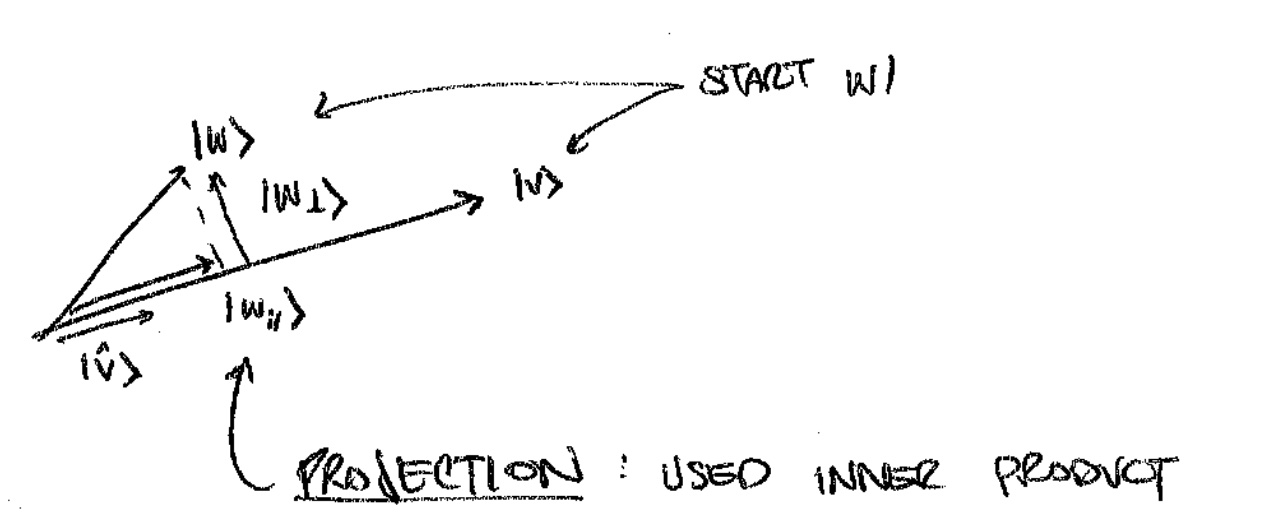
\includegraphics[width=.8\textwidth]{figures/gram-projection.jpg}
    \caption{Projection of a vector $\ket{w}$ onto the axis of another vector, $\ket{v}$.}
    \label{fig:gram:projection}
\end{figure}

Our strategy is to separate the ket $\ket{w}$ into a piece that is parallel to $\ket{v}$ and a piece that is perpendicular to $\ket{v}$. We will call these pieces:
\begin{align}
    \ket{w}= \ket{w_\paral} + \ket{w_\perp} \ .
\end{align}
The defining characteristic of $\ket{w_\paral}$ is that $\la \hat{w}_\paral, \hat{v}\ra = 1$. That is: the angle between the unit vectors is zero---they are parallel. This means that 
\begin{align}
    \ket{w_\paral} \propto \ket{\hat{v}} \ .
\end{align}
What is the proportionality? This is simply the length of $\ket{w}$ along the $\ket{\hat{v}}$ axis, which we know from Example~\ref{eg:component:along:an:axis} is the inner product:
\begin{align}
    \ket{w_\paral} = \la w, \hat{v} \ra \ket{\hat{v}} =  \ket{\hat{v}}\la \hat{v}, w \ra  \ .
\end{align}
In the last line we decided to be silly: since the inner product of two kets is simply a number, we can place it to the right of the ket $\ket{\hat{v}}$. Let us say that this is for aesthetic reasons for now. Then let us recall \eqref{eq:inner:product:row:vector} which related an inner product with $\ket{v}$ to a contraction with $\bra{v}$. We thus write:
\begin{align}
    \ket{w_\paral} = \ket{\hat{v}} \la{\hat{v}} | w \ra  =
    \left(\ket{\hat{v}} \bra{\hat{v}} \right)  \, \ket{w} \ .
     \ .
\end{align}
Here we recognize that the terms in parenthesis are simply the form of a \emph{matrix}, a linear transformation that eats a ket and returns a ket, see \eqref{eq:matrix:in:ket}. Evidently $\ket{\hat{v}} \bra{\hat{v}}$ is the matrix that takes $\ket{w}$ and returns $\ket{w_\paral}$, the component of $\ket{w}$ along $\ket{\hat{v}}$. In this language, it is somewhat \emph{obvious} that this is what $\ket{\hat{v}} \bra{\hat{v}}$ does. However, we have not written the components of $\ket{\hat{v}} \bra{\hat{v}}$ in terms of our standard basis. To do that, one simply expands each  of $\ket{\hat{v}}$ and $\bra{\hat{v}}$ in the standard basis. One may invoke linearity to read off the components of the projection matrix, $P = P\aij{i}{j}\ket{i}\bra{j}$, as seen in the following examples. 

\begin{example}
First a simple warm up. Consider the vectors
\begin{align}
    \ket{v} &= 2.5 \ket{1}
    &
    \ket{w} &= 3\ket{1} + 4\ket{2} \ .
\end{align}
We want to find $\ket{w_\paral}$. First we identify the unit vector in the $\ket{v}$ direction, which is simply $\ket{\hat{v}} = \ket{1}$. As a matrix, the projection operator $P = \ket{\hat{v}} \bra{\hat{v}}$ is
\begin{align}
    \ket{\hat{v}} \bra{\hat{v}} = \ket{1}\bra{1} 
    &=
    \begin{pmatrix}
        1 & \\
        & 0
    \end{pmatrix}
    \ .
\end{align}
Int he last step we have matched the components to  $P = P\aij{i}{j}\ket{i}\bra{j}$.
Applying this to $\ket{w}$ gives
\begin{align}
    \ket{\hat{v}} \bra{\hat{v}}w\ra = \ket{1}\bra{1}\left(3\ket{1}+ 4\ket{2}\right)
    = 3 \ket{1} \ .
\end{align}
\end{example}

\begin{example}
Here is a less-simple example. Consider the vectors
\begin{align}
    \ket{v} &= \sqrt{3} \ket{1} + \ket{2}
    &
    \ket{w} &= 3\ket{1} + 4\ket{2} \ .
\end{align}
We want to find $\ket{w_\paral}$. As a hint, the coeffients of $\ket{v}$ were chosen to be reminiscent of a 30-60-90 degree triangle. The unit vector in the $\ket{v}$ direction is
\begin{align}
    \ket{\hat{v}} 
    &= 
    \frac{\sqrt{3}}{2} \ket{1} + \frac{1}{2} \ket{2} \ .
\end{align}
As a matrix, the projection operator $P = \ket{\hat{v}} \bra{\hat{v}}$ is
\begin{align}
    \ket{\hat{v}} \bra{\hat{v}}
    &=
    \left(\frac{\sqrt{3}}{2}\bra{1} + \frac{1}{2} \bra{2}\right)
    \left(\frac{\sqrt{3}}{2}\ket{1} + \frac{1}{2} \ket{2}\right)
    \\
    &=
    \frac{3}{4}\ket{1}\bra{1}
    \frac{\sqrt{3}}{4}\ket{2}\bra{1}
    \frac{\sqrt{3}}{4}\ket{1}\bra{2}
    \frac{1}{4}\ket{2}\bra{2}
    \\
    &=
    \frac{1}{4}
    \begin{pmatrix}
        3 & \sqrt{3} \\
        \sqrt{3} & 1
    \end{pmatrix}
    \ .
\end{align}
Observe that the determinant of $\ket{\hat{v}} \bra{\hat{v}}$ is zero. We will see that this is a feature of projection matrices that ``throw out'' information. In this case, $\ket{\hat{v}} \bra{\hat{v}}$ has thrown out information about the perpendicular direction, $\ket{w_\perp}$.
\end{example}

\begin{exercise}
Draw the vectors $\ket{v}$ and $\ket{w}$. You should recognize that $\ket{w}$ is $\pi/6$ (30~degrees) counterclockwise of $\ket{v}$. This means that if we rotated the system by this amount in the clockwise direction, the above example should reduce to projection onto the $\ket{1}$ axis, which was our ``easy'' example above. The appropriate rotation matrix is
\begin{align}
    R = 
    \begin{pmatrix}
        \cos(-\pi/6) & -\sin(-\pi/6)
        \\
        \sin(-\pi/6) & \pp\cos(-\pi/6)
    \end{pmatrix}
    = 
    \frac{1}{2}
    \begin{pmatrix}
        \sqrt{3} & 1 \\
        -1 & \sqrt{3}
    \end{pmatrix} \ .
\end{align}
Further, recall how a matrix transforms under a rotation. If you do not remember, please go back and review Section~\ref{sec:transformation:of:matrices}. Go ahead and do it. I'll wait here. Yes, it is \emph{that} important. We see that the components of $P = \ket{\hat{v}} \bra{\hat{v}}$ transform as
\begin{align}
    P\aij{i}{j}\to (P')\aij{i}{j} = R\aij{i}{k} P\aij{k}{\ell} (R^{-1})\aij{\ell}{j}\ .
\end{align}
Do not forget that the inverse of a rotation is simply its transpose. Show that the only non-zero component of $P'$ is $(P')\aij{1}{1} = 1$. Thus $P'$ is indeed a projection onto the $x$-axis.
\end{exercise}

\begin{bigidea}\label{bigidea:multiply:by:one}
The ket-bra notation for matrices gives a nice representation of the unit matrix:
\begin{align}
    \one = \sum_i \ket{i}\bra{i}  \ .
\end{align}
In quantum mechanics we say that we \emph{insert a complete set of states}. All that means is that we're multiplying by one. Keep this in mind for later. The significance of this ``multiply by one'' operation is that it is true no matter what basis $\ket{i}\bra{i}$ is written in. We will use ``multiplication by one'' judiciously to convert from one basis to another. 
\end{bigidea}

\begin{example}
Consider the following bases:
\begin{align}
    \ket{1'} &= \frac{1}{\sqrt{2}}\ket{1} - \frac{1}{\sqrt{2}}\ket{2}
    &
    \ket{2'} &= \frac{1}{\sqrt{2}}\ket{2} + \frac{1}{\sqrt{2}}\ket{2} \ .
\end{align}
This is clearly a rotation by $\pi/4$. What are the components of $\ket{v} = \ket{1} + \ket{2}$ in the primed basis? The answer should be obvious either from inspection or by drawing a picture. Let us see how to calculate this by ``multiplying by one'':
\begin{align}
    \ket{v} = \one\ket{v} = \left(\ket{1'}\bra{1'} + \ket{2'}\bra{2'}\right)\; \left(\ket{1} + \ket{2}\right) \ .
\end{align}
Now we use the overlaps:
\begin{align}
    \la 1' | 1 \ra &= \frac{1}{\sqrt{2}}
    &
    \la 1' | 2 \ra &= \frac{-1}{\sqrt{2}}
    &
    \la 2' | 1 \ra &= \frac{1}{\sqrt{2}}
    &
    \la 2' | 2 \ra &= \frac{1}{\sqrt{2}} \ .
\end{align}
This gives  
\begin{align}
    \ket{v} = \frac{1}{\sqrt{2}}
    \left(
        \ket{1'} - \ket{2'} + \ket{1'} + \ket{2'}
    \right)
    = 
    \frac{2}{\sqrt{2}}\ket{1'} \ .
\end{align}
As expected from their definitions, $\ket{v}$ is along the $\ket{1'}$ direction.
\end{example}

\subsection{Inverse Metric}

The metric has an inverse, $g^{-1}$.  If we think of the metric as a machine that lowers indices, the inverse metric raises indices. This should already tell you that the index structure of the inverse metric is $(g\inv)^{ij}$. By virtue of being an inverse, we expect that acting with the metric and then its inverse---or the reverse order---returns you to the original tensor:
\begin{align}
    g_{ik}(g\inv)^{kj} = (g\inv)^{jk}g_{ki} = \delta^j_i \ .
\end{align}
Note that $(g\inv)^{ij}$ is symmetric because it inherits this symmetry from $g$. Because we are \sout{lazy} \emph{practical}, we recognize that there is never any ambiguity about whether we are using $g$ or $g\inv$. If you know a tensor $T$ and then you see some component that looks like the components of $T$ except one of the indices is upper rather than lower, then you know that that index was raised by contracting $g\inv$. Similarly, if an index that you expected to be upper turns up lowered, then you know that the index was lowered by contracting with $g$. Thus we usually do not bother writing $g\inv$, leaving it implicit unless there is some ambiguity.

In fact, we can go further. In the rare cases when we \emph{do} explicitly write out the inverse metric, we go ahead and drop the $\inv$. This is because we can tell from the index structure whether we are using $g$ or $g\inv$. So we now set the convention:
\begin{align}
    g^{ij} \equiv (g\inv)^{ij} \ .
\end{align}

\begin{example}
The following is a metric and inverse-metric pair:
\begin{align}
    g_{ij} &= 
    \begin{pmatrix}
        1 & \\ & 3
    \end{pmatrix}
    &
    g_{ij} &= 
    \begin{pmatrix}
        1 & \\ & 1/3
    \end{pmatrix}\ .
\end{align}
As always, we are writing the \emph{components} of these tensors. Do not confuse these as ``matrices,'' see \bigidearef~\ref{idea:treating:two:index:as:matrix}.
\end{example}



\subsection{Isometries: A Fancy Name For Rotations}\label{sec:rotations:isometries}

Section~\ref{sec:rotations} highlighted the significance of rotations in $\RR^2$ and $\RR^3$. What was not evident was \emph{why} rotations are so important and where they came from mathematically. Now that we have defined the metric, we can define rotations in Euclidean space and their generalization to any metric space.

Let $R$ be an invertible transformation---not necessarily a rotation. The inner product of two vectors is $g(\vec{v},\vec{w})$. Under the transformation the vectors each transform as $\vec{v}\to \vec{v}'= R\vec{v}$ and $\vec{w} \to\vec{w}'= R\vec{w}$. The metric---a two component tensor with lower indices---also transforms, $g_{ij} \to g'_{ij}$. How does it transform? Recalling how we derived the transformation of matrices in Section~\ref{sec:transformation:of:matrices}, let us require that $g(\vec{v},\vec{r}) = g'(\vec{v}', \vec{w}')$:
\begin{align}
    % g(\vec{v}, \vec{w}) = g_{ij}v^i w^j \to 
    % g'(\vec{v}', \vec{w}') = 
    g'_{ij} (v')^i (w')^j 
    %\quad = \quad
    &=
    g_{k \ell} v^k w^\ell
    = g_{k\ell} (R\inv)\aij{k}{i}(v')^i (R\inv)\aij{\ell}{j}(v')^j \ .  
\end{align}
Peeling off the $(v')^i$ and $(w')^j$ on both sides\footnote{Recall that ``peeling off'' is not a valid mathematical operation. What we really mean is that because the equality holds for any $v'$ and $w'$, the prefactors must match. Note that we labelled our dummy indices in a convenient way to do this ``peeling off.''} gives
\begin{align}
    g'_{ij} = g_{k\ell} (R\inv)\aij{k}{i} (R\inv)\aij{\ell}{j}
    = 
    (R\inv)\aij{k}{i} g_{k\ell}  (R\inv)\aij{\ell}{j} \ .
    \label{eq:gp:RgR}
\end{align}
For simplicity, define $\bar R = R\inv$. We shall now define the properties that will make $\bar R$ a rotation---if $\bar{R}$ is a rotation then its inverse $R$ is also a rotation. Let us write \eqref{eq:gp:RgR} as ``matrix multiplication,'' by which we mean that consecutive indices are contracted. As we exhorted in \bigidearef~\ref{idea:treating:two:index:as:matrix}, this does not mean that $g$ has the tensorial structure of a matrix (it does not), only that we are writing the components as a $2\times 2$ array such that the index contractions aligns with the grade-school notion of matrix multiplication:
\begin{align}
    g'_{ij} &= (\bar R^T)_i^{\phantom{i}k} g_{k\ell} \bar R\aij{\ell}{j} 
    \label{eq:gp:RT:g:R}
\\ &=
    \begin{pmatrix}
        \bar R\aij 11 & \bar R\aij 21 \\
        \bar R\aij 12 & \bar R\aij 22 
    \end{pmatrix}
    \begin{pmatrix}
        g_{11} & g_{12}\\
        g_{22} & g_{22}
    \end{pmatrix}
    \begin{pmatrix}
        \bar R\aij 11 & \bar R\aij 12 \\
        \bar R\aij 21 & \bar R\aij 22 
    \end{pmatrix}
    \ .
\end{align}
In the first rotation matrix we used $(\bar R^T)_1^{\phantom{1}2} = \bar{R}\aij{2}{1}$. We say that the transformation $R$ is an \textbf{isometry} if $g'_{ij} = g_{ij}$. 

Let us consider the case when $g_{ij}$ is the Euclidean metric. This means that the components $g_{ij}$ are the components of the identity matrix, $\one$. Then then plugging in $g'_{ij} = g_{ij}$ into \eqref{eq:gp:RT:g:R} gives a matrix equation for the components of $\bar R$:
\begin{align}
    \one &= \bar R^T \one \bar R = \bar R^T 
    &\Rightarrow
    &&
    {\bar R}\inv = {\bar R}^T
    \ .
    \label{eq:rotation:definition:one}
\end{align}
This is the \emph{definition} of a rotation: it is an isometry of Euclidean space. Even though we have shown that $\bar R = R\inv$ is a rotation, we know that this imposes that the transformation on vectors, $R = \bar R\inv$, is also a rotation since it is simply a transformation in the opposite direction as $\bar R$.
\begin{exercise}
Show that for $\RR^2$ with the Euclidean metric, the condition \eqref{eq:rotation:definition:one} imposes a generic form
\begin{align}
    \bar R = 
    \begin{pmatrix}
        \pp \cos\theta & \sin\theta\\
        - \sin\theta & \cos\theta  
    \end{pmatrix}
    \ .
\end{align}
It may help to remember that $\cos^2\theta + \sin^2\theta = 1$.
\end{exercise}


\textbf{Isometries} are special transformations. Because they leave the metric unchanged, they also preserve the orthonormality of a basis. Under an isometry, an orthonormal basis is transformed into another orthonormal basis. We will make ample use of this: there is often a ``most convenient basis'' in which the action of a given matrix simplifies tremendously. Physically, these isometries correspond to a shift in observer. It just goes to show: sometimes the easiest way to solve a problem is to change your perspective.
\begin{exercise}
Show that if  $\bas{e}_i$ is an orthonormal basis, then its transformation under an isometry $R$ is still an orthonormal basis.
\end{exercise}



\begin{exercise}\label{ex:minkowski:2}
Considering the Minkowski metric for (1+1)-dimensional spacetime:
\begin{align}
    g_{\mu\nu} &= 
    \begin{pmatrix}
        1 & \pp 0\\
        0 & -1
    \end{pmatrix} \ .
\end{align}
We have used $\mu$ and $\nu$ indices as is conventional for relativity. Following this convention of $R$, we write $\Lambda$ for the isometries of Minkowski space. Show that the following forms of $\Lambda$ satisfy the isometry condition, $\Lambda^T \Lambda = \one$:
\begin{align}
    \Lambda = 
    \begin{pmatrix}
        \cosh\eta & \sinh\eta \\
        \sinh\eta & \cosh\eta\\
    \end{pmatrix}
    = 
    \begin{pmatrix}
        \gamma & \gamma\beta\\
        \gamma\beta & \gamma
    \end{pmatrix} \ ,
\end{align}
where $2\cosh\eta = e^{\eta}+e^{-\eta}$, $2\sinh\eta = e^{\eta}-e^{-\eta}$, and $\gamma^2 = (1-\beta^2)^{-1/2}$. It may help to know that $\cosh^2\eta-\sinh^2\eta = 1$. The isometry $\Lambda$ is called a Lorentz transformation.
\end{exercise}


\begin{bigidea}\label{eq:rotations:generalized}
Isometries are the generalization of rotations. These are defined by transformations that leave the metric unchanged. In what follows, we will use the word `isometry' and `rotation' interchangeably. These generalized rotations form a set of transformations that let us go from one orthonormal basis to another. 
\end{bigidea}

Here's a nice little aside. The isometries that we have met so far all have some continuous transformation parameter. Rotations in $\RR^2$ are defined by  a rotation angle $\theta$. In more Euclidean dimensions there are more rotation angles. These rotation angles can take any real value. Even the boosts have a continuous parameter: this is either the rapidity, $\eta$, or the velocity in units of the speed of light, $\beta = v/c$. Compositions of isometries are simply another isometry: a rotation by $\theta_1$ and then $\theta_2$ is a rotation by $(\theta_1+\theta_2)$. A few ``beyond the scope of this class'' comments are worth highlighting since they will show up in your physics life:
\begin{enumerate}
    \item Other than the simplest cases, the order in which one composes isometries matters. For an explicit example, see Fig.~\ref{fig:rotate:QFT}.
    \item The \emph{way} in which the order of isometries matters reflects an underlying mathematical structure of the isometries. 
    \item Isometries are \emph{symmetries} of a physical system. 
    \item The theory of symmetries with continuous parameters and its application to physical systems is called the representation theory of Lie groups. 
\end{enumerate}


% Isometries form a group: 
% g_{ij}R\aij{i}{k}R\aij{j}{\ell}v^k w^\ell

% An \textbf{isometry} is a linear transformation from $V\to V$ that leaves the metric unchanged. Recalling how tensors with two lower indices transform, under a transformation $S$ the metric transforms

% as symmetries Isometries
% notation of change of variables

% talk about matrix notation. THis is not literally matrix notation. It's a table whose multiplicaiton means something.

\subsection{The meaning of indices}

Having rigorously defined isometries as ``generalized rotations'' for a given metric, we can now reflect on the significance of our index notation. We proposed that the index pattern of a tensor's components indicates how the components transform under rotations. This is generalized to the statement that the indices of an object indicate how it transforms under isometries. Because isometries preserve the metric, they naturally map between different orthonormal bases. These orthonormal basis represent different `reference frames' in which a physical system is described. By rotating (isometry-ing) to a convenient basis, one can often convert a challenging problem into a much simpler problem.  

It is a bit of a joke in physics that there is a standard definition for what a tensor is:
\begin{quote}
A tensor is an object that transforms like a tensor.
\end{quote}
This is not an obviously useful definition, though it does highlight the significant piece for physicists: transformation laws. Mathematicians often find this definition silly. The `proper' definition of a tensor is that it is a multi-linear map between vector spaces. Further, mathematicians will scoff at our emphasis on isometries (rotations): they will say \emph{hey, you, physicists: don't you see that tensors will transform `like a tensor' for any invertible transformation? Why are you so obsessed with isometries?}

\begin{exercise}
Confirm what our mathematician friend is saying. Suppose you have a general tensor with $p$ upper indices and $q$ lower indices.\footnote{You can always start some specific index structure and see how the result generalizes.} Further, suppose that your vectors transform under an invertible transformation $M$, $\ket{v}\to M\ket{v'}$. Under this transformation, argue that row vectors transform with $M\inv$, and further that the general tensor transforms as in \eqref{eq:transformation:of:tensor} with the rotation matrix $R(\theta)$ replaced by the general invertible matrix $M$. You may want to follow the rough steps in Section~\ref{sec:transformation:of:matrices} where we motivated the transformation law for matrices.
\end{exercise}

So why are we making a big deal about isometries? Isometries physically correspond to a change in observer. As physicists, we would like to deduce the fundamental laws of nature---laws that we expect to be independent whether we are oriented along a particular direction in space or in a particular reference frame. Isometries are transformations that translate the physical quantities that one observer measures to the physical quantities that another observer measures. The physical quantities are encoded in the components of tensors and the fact that those components transform indicate what a different observer would measure.

In this sense, it is true that you could do an arbitrary invertible transformation\footnote{Invertibility is important to make sense of the transformation of lower-indices.} and this all holds. However, a transformation that is not an isometry will change the metric. This means the transformation maps an orthonormal basis to a non-orthonormal basis.\footnote{Convince yourself that the condition of invertibility ensures that the orthonormal basis is at least mapped to a basis.} This means that the transformed basis is not meaningful as the basis vectors that another physical observer may measure---at least not a sensible physical observer with a sensible basis.

\subsection{Transpose, Adjoint}
\label{eq:transpose:adjoint}

In our discussion so far, we have made use of a `colloquial' definition of the transpose of a matrix: $(M^T)\aij{i}{j} = M_j^{\phantom{j}i}$. What dictated the index height? Thus far we have been glib about this because we have not had to use a careful definition of the transpose. Now that we have a metric, we can be more rigorous. The \textbf{adjoint} of a linear transformation $A$ is defined to be $A^\dag$ such that
\begin{align}
    \la A^\dag \vec{v}, \vec{w} \ra \equiv
    \la \vec{v} , A \vec{w} \ra \ .
\end{align}
\begin{example}
By the symmetry of the metric we could have equivalently written
\begin{align}
    \la A^\dag \vec{v}, \vec{w} \ra =
    \la \vec{v} , A \vec{w} \ra =
    \la \vec{w}, A^\dag \vec{v} \ra =
    \la A \vec{w}, \vec{v} \ra 
    \ .
\end{align}
The point of the metric is \emph{not} that you're moving the matrix $A$ from one slot to the other, it is that you are changing from a transformation $A$ that acts on $\vec{v}$ to a transformation $A^\dag$ that acts on the \emph{other} input vector $\vec{w}$ defined such that the inner product is the same.
\end{example}
When $A$ is a real matrix, $A^\dag \equiv A^T$. What does this mean? Write out the components of each side:
\begin{align}
    \la A^\dag \vec{v}, \vec{w} \ra
    &=
   w^k \, g_{ki}  (A^\dag)\aij{i}{\ell} v^\ell  \,  
    &
    \la  \vec{v},A \vec{w} \ra
    &=
   v^\ell\, g_{\ell j}  A\aij{j}{k} w^k  
   \ .
\end{align}
Now set these two inner products equal to each other gives
\begin{align}
    g_{ki}(A^\dag)\aij{i}{\ell}
    &=
    g_{\ell j} A\aij{j}{k}
\end{align}
Contracting both sides with the inverse metric $g^{km}$ gives
\begin{align}
    (A^\dag)\aij{m}{\ell} &= g_{\ell j} A\aij{j}{k} g^{km} \ .
    \label{eq:adjoint:def}
\end{align}
This relation \emph{defines} the adjoint. Observe that when the metric is diagonal (say for the Euclidean metric), the first index of $A^\dag$ is a contraction of the {second} index of $A$ and the second index of $A^\dag$ is a contraction of the first index of $A$. In this sense, the order of the indices have swapped. 

Ah! But we already have a familiar operation that swaps the order of indices: the transpose, which we defined for [Euclidean] $\RR^N$ in \eqref{eq:transpose:components} to be $(M^T)\aij{i}{j} = M\aij{j}{i}$. Let us give a formal definition: When the vector space is real, the adjoint is the \textbf{transpose} of a matrix.  
%
We can read this off of \eqref{eq:adjoint:def} when we use\footnote{Please understand what the following statement means. Normally it is dangerous to write equations where the indices on the left-side do not match the indices on the right-side. What we're saying here is that the \emph{components} of $g$ and $g^{-1}$---but not necessarily the tensor structure (upper or lower)---match the components of the identity. Again, we refer back to the subtle point in \eqref{idea:treating:two:index:as:matrix}.} $g_{ij} = g^{ij} = \mathbbm{1}$. 

What about the height of the indices? In the non-rigorous definition of the transpose, there is a potential ambiguity on the height of the indices. If $M=M\aij{i}{j}\ket{i}\bra{j}$:
\begin{align}
    M^T \stackrel{?}{=} 
    \begin{cases}
    (M^T)\aij{j}{i}\ket{j}\bra{i}    & \text{ or }\\
    (M^T)_{j}^{\phantom{j}i}\ket{i}\bra{j}
    \end{cases}
    \quad\text{.}
\end{align}
This ambiguity came up in \eqref{eq:ABC:matrix:multiplication:tensor:note}, where we glibly wrote $(A^T)_i^{\phantom{k}i} = A\aij{k}{i}$ and apologized that  this was not quite formally correct---especially since the fact that the ``first upper then second lower'' index pattern appears to be violated.  We now see that the index structure of the transpose of a matrix is preserved: the transpose of a matrix is a matrix. That is to say: a matrix has its first index upper and the second index lower. The transpose has the same pattern. 

We see how this happens: the first (upper) index of $A$ becomes the second index of $A^T$. However, we want the second index of $A^T$ to be \emph{lower}. How do we manage this? The metric gives us precisely the tool to lower indices. We see that this is exactly what happens in \eqref{eq:adjoint:def}: we use the metric and its inverse to ensure that the heights of the $A^T$ indices match that of an ordinary matrix. This had to be since our definition \eqref{eq:adjoint:def} has $A^T$ acting on a vector, so we expect $A^T$ to be an ``ordinary'' linear transformation.

\begin{exercise}
In your own words, articulate the difference between a matrix $A$, its inverse $A\inv$, and its transpose $A^T$. What if $A$ is a rotation?
\end{exercise}

\begin{exercise}
Show that taking the adjoint twice returns you to the original matrix, $(A^\dag)^\dag = A$.
\end{exercise}

\begin{example}
The transpose/adjoint also gives us a way to understand why isometries act differently on column vectors (ket) versus row vectors (bra). The metric lets us convert a column vectors into row vectors, as we saw in Section~\ref{sec:machine:to:make:row:vectors}. Start with a vector $\ket{v}$ with components $v^i$. Under a rotation, these components become $(v')^i = R\aij{i}{j}v^j$. From the transformed ket $\ket{v'} = (v')^i \ket{i}$ we invoke the metric to convert this into a bra:
\begin{align}
\bra{v'} = \la v', \smallslot \ra = \la \smallslot, v' \ra \equiv v'_i \bra{i} \ .    
\end{align}
In the last line we have implicitly used the metric: we have a definition for $(v')^i$, so the meaning of $(v')_i$
is understood to be
\begin{align}
    (v')_i = g_{ij} R\aij{j}{k}v^k \ .
\end{align}
What are the components of $(v')_i$ relative to $v_i$? To do that we can insert $\one$ in a clever way:
\begin{align}
    g^{mn}g_{n\ell} = \delta^m_\ell
\end{align}
so that 
\begin{align}
    (v')_i = g_{ij} R\aij{j}{k} g^{k\ell}g_{\ell m} v^m
    = 
    \left(g_{ij} R\aij{j}{k} g^{k\ell}\right)
    v_\ell
    = 
    v_\ell(R^\dag)\aij{\ell}{i} 
    \ ,
\end{align}
where again we have implicitly \emph{defined} $v_\ell = g_{\ell m}v^m$. That's just what metrics do. That's what they \emph{do}.\footnote{\url{https://www.youtube.com/watch?v=Akq0xeu-RHE}} In the last equality we recognize the definition of the adjoint, \eqref{eq:adjoint:def}. In our case of a real metric space, of course, this is simply $R^\dag = R^T$. This confirms for us that the objects with lower indices transform by contracting with $R^\dag$, which we identified in \eqref{eq:rotation:definition:one} to be the inverse of the rotation $R$. So there you have it: objects with lower indices transform with $R\inv = R^\dag$. 

We can do a sanity check for this. The inner product is a number and should not transform under rotations. We can see what happens:
\begin{align}
    \la v , w \ra \to \la Rv, Rw \ra = \la v, R^\dag R w \ra = \la v, w \ra \ .
\end{align}
where we used $R^\dag R = \one$. 




% Starting with a ket $\ket{v}$, we define the bra
% \begin{align}
% \bra{v} = \la v, \smallslot \ra = \la \smallslot, v \ra \ .    
% \end{align}
% Now act $\bra{v}$ on a ket $\ket{w}$. By linearity, I can also transform the ket by a matrix $A$ and then feed $\ket{Aw}=A\ket{w}$ to $\bra{v}$:
% \begin{align}
%     \la{v} | {Aw} \ra = \bra{v}A \ket{w} = \la v, Aw \ra \equiv \la A^\dag v, w\ra = \bra{A^\dag v} w\ra \ .
% \end{align}
% Now suppose $A$ is an isometry. Assuming that the space is real\footnote{That is: every time we say `number' we mean a \emph{real} number, $\RR$.} and that we have the Euclidean metric, this is simply the assumption that $A=R$, a rotation. 
\end{example}


\subsection{Complex metric spaces}

\paragraph{Complex vector spaces}
It is time to embrace complex numbers. A complex vector space is one where all of the numbers that we previously assumed were real can now be complex: $\RR \to \CC$. This means that a linear combination of vectors $\alpha\vec{v}+ \beta\vec{w}$ may have complex coefficients, $\alpha,\beta\in\CC$. 

\paragraph{Quick refresher of complex numbers}
Recall that complex numbers may be written either in Cartesian form, $z = x+iy$ or in polar form $z= re^{i\theta}$. The defining features is that $i^2 = -1$. The complex conjugate of a complex number is the complex number you get from changing $i\to -i$:
\begin{align}
    (x+iy)^* &= x-iy
    &
    re^{i\theta} &= re^{-i\theta} \ .
\end{align}

\paragraph{Metrics on complex spaces}
Things become a bit more interesting when we complexify a metric space. We have to update our rules a bit. Previously we assumed that the metric is symmetric, $\langle v, w\rangle = \langle w, v\rangle$. This turns out to only be true for real spaces. When we have a complex vector space, the metric must satisfy symmetry with a complex conjugation:
\begin{align}
    \la v, w \ra = \la w, v \ra^* \ .
\end{align}
That is a little unusual. At least means that the norm (length squared) of a complex vector is real:
\begin{align}
    |v|^2 = \la v, v \ra = \la v, v \ra^* \ .
\end{align}
This helps justify the notation $|v|$ for the magnitude of a vector. 

What about the adjoint of a transformation? For a real vector space, the adjoint is simply the transpose. For a complex vector space, the adjoint is the transpose \emph{and} a complex conjugation on each component:
\begin{align}
    (A^\dag)\aij{i}{j} = g^{ik}(A\aij{\ell}{k})^*g_{\ell j} \ .
\end{align}
In terms of components:
\begin{align}
    \begin{pmatrix}
        A\aij 11 & A\aij 12 \\
        A\aij 21 & A\aij 22 
    \end{pmatrix}^\dag &= 
    \begin{pmatrix}
        (A\aij 11)^* & (A\aij 21)^* \\
        (A\aij 12)^* & (A\aij 12 )^*
    \end{pmatrix} \ .
\end{align}
\begin{example}
Here's the adjoint of an explicit matrix:
\begin{align}
\begin{pmatrix}
        3.5 +2i & 2.3+7i \\
        8.3 + 5i & 5-2i
    \end{pmatrix}^\dag &= 
    \begin{pmatrix}
        3.5 -2i &  8.3 - 5i\\
        2.3 -7i & 5 +2i
    \end{pmatrix} \ .
\end{align}
\end{example}

\begin{example} What do isometries look like in a complex vector space? Let us suppose that we have the Euclidean metric (even though the space is now complex):
\begin{align}
    g_{ij} = \text{diag}(1,1,\cdots, 1) = \mathbbm{1} \ .
\end{align}
Let $U$ be an isometry in this space; this is a conventional name whose meaning will be clear soon. The condition for an isometry in this space is that a transformation $\ket v \to U\ket{v}$ preserves the metric. Observe that because the metric is not symmetric, but rather symmetric-up-to-a-conjugate, it is useful to write the inner product using brackets rather than simply index contraction. We have:
\begin{align}
    \la U\vec{v}, U\vec{w} \ra = \la \vec{v}, U^\dag U \vec{w} \ra \stackrel{?}{=} \la \vec{v}, \vec{w} \ra \ .
\end{align}
This tells us that the condition for $U$ to be an isometry is that $U^\dag U = \mathbbm{1}$. Matrices that satisfy this are called \textbf{unitary} matrices, thus justifying the name $U$. 
\end{example}

\begin{example}
The usual rotation matrices (obviously!) satisfy the unitary condition. Thus rotations are a simple example of a unitary matrix. There are more complicated unitary matrices, for example in two complex dimensions:
\begin{align}
    U(\theta) = 
    \begin{pmatrix}
        e^{i\theta} & 0\\
        0 & e^{-i\theta}
    \end{pmatrix}
    \label{eg:unitary:matrix:diagonal}
\end{align}
is a transformation that rephases the first $v^1 \to e^{i\theta}v^1$  and second $v^2 \to e^{-i\theta}v^2$ components of a vector by opposite phases. It should be obvious that $U^\dag U = \one$. 
\end{example}


\begin{exercise}
A bonus observation: show that \eqref{eg:unitary:matrix:diagonal} can be understood as a Taylor expansion with respect to a matrix $T$:
\begin{align}
    U(\theta) &= \sum_{n=0}^\infty \frac{\theta^n}{n!} T^n
    &
    T=
    \begin{pmatrix}
        i & 0\\
        0 & -i
    \end{pmatrix} \ .
\end{align}
The matrix $T$ is called the \textbf{generator} of the isometry $U$. 
\end{exercise}


\begin{exercise}
Show that the generator of rotations is
\begin{align}
    R(\theta) &= \sum_{n=0}^\infty \frac{\theta^n}{n!} T^n
    &
    T=
    \begin{pmatrix}
        0 & -1\\
        1 & \pp 0
    \end{pmatrix} \ .
\end{align}
\end{exercise}


% \begin{table}
%     \renewcommand{\arraystretch}{1.3} % spacing between rows
%     \centering
%     \begin{tabular}{ @{} llllll @{} } \toprule % @{} removes space
%         Space
%         & Numbers
%         & Inner Product
%         & Contraction
%         & Matrix
%         & Identity
%         \\ \hline
%         Classic
%             & vector
%             & row-vector
%             & 
%             &       
%         \\
%             & $\vec{v} = v^i \bas{e}_i$
%             & $\row{w} = w_i \rbas{e}^i$
%             & $\rbas{e}^i\bas{e}_j = \delta^i_j$
%             & $M=M\aij{i}{j} \bas{e}_i\otimes \rbas{e}^j$
%             & $\one$
%         \\ \hline
%         Quantum 
%             & ket
%             & bra
%             &       
%             &
%         \\
%             & $\ket{v} = v^i\ket{i}$
%             & $\bra{w} = w_i \bra{i}$
%             & $\langle i | j\rangle = \delta^i_j$
%             & $M=M\aij{i}{j} \ket{i}\bra{j}$
%             & $\ket{i}\bra{i}$
%         \\ \bottomrule
%     \end{tabular}
%     \caption{
%         Dictionary between `classic' notation and `quantum' (bra--ket) notation.
%         \label{tab:classic:bra:ket:dictionary}
%     }
% \end{table}

\subsection{Gram--Schmidt}

The metric allows us to determine whether a basis is orthonormal or not. We \emph{like} orthnormal bases. Sometimes life gives us garbage bases that are not orthonormal. What are we to do? The Gram--Schmidt procedure is a way to use the metric to take any basis and convert it into an orthonormal basis. We already met the key ideas in Section~\ref{sec:projections}. Here we focus on the two dimensional case. Refer back to Fig.~\ref{fig:gram:projection}: we have two vectors, $\ket{v}$ and $\ket{w}$. How do we turn these into two orthonormal basis vectors?
%
The general procedure is:
\begin{enumerate}
    \item Grab one vector from the pile of garbage basis vectors. Normalize this vector and stick it in your bag of nice basis vectors. 
    \item Grab another vector from the pile. Do whatever you need to do to make it fit as a nice basis vector with the other nice basis vectors in your bag. This means that you have to find what new `direction' the vector identifies relative to the existing basis vectors, and then you have to normalize the component of the vector along that direction. That normalized vector is perpendicular to the other basis vectors and can now be placed in the bag of nice basis vectors.
    \item Repeat the previous step until you have a complete basis. 
\end{enumerate}

We can start with $\ket{v}$ and simply normalize it: $\ket{\hat{v}} = \bas{e}_1$ is the first basis vector. The next step is to pull out the perpendicular part of $\ket{w}$. In Section~\ref{sec:projections} we saw how to do this: simply decompose
\begin{align}
    \ket{w} &= \ket{w_\paral} + \ket{w_\perp}
    &
    \ket{w_\paral} &=  \bra{\hat v}\la \hat v \ket{w} \ .
\end{align}
This gives us $\ket{w_\perp}$ in terms of two vectors $\ket{w}$ and $\ket{w_\paral}$ that we know. We can thus normalize this and that gives us the second vector: $\ket{\hat{w}_\paral} = \bas{e}_2$. If you have more vectors, then continue until you are out. When you identify the perpedicular part, $\ket{u_\perp}$, you have to make sure that $\ket{u_\perp}$ is perpendicular to \emph{all} of the earlier basis vectors:
\begin{align}
    \la \bas{e}_1, u_\perp \ra =
    \la \bas{e}_2, u_\perp \ra =
    0 \ .
\end{align}



\begin{exercise}
Would you have the same basis vectors if you started with $\ket{w}$ and then took the perpendicular part of $\ket{v}$?
\end{exercise}



\section{Special Relativity: Minkowski Space}

% Ex: show that the norm of a vector is preserved under lorentz

Minkowski spacetime is the metric space for special relativity. The Minkowski metric is similar to the Euclidean metric, except that the time-like dimensions have a negative sign relative to the space-like dimensions. We say that a spacetime is (3+1)-dimensional when there are three dimensions of space and one dimension of time.\footnote{Which dimensions are space and which dimensions are time are mathematically a matter of convention. The physically significant fact is that there is a relative sign. It is rather unusual to have more than one time dimension. There are some cases where you may use two time dimensions as a crutch---look up anti-de~Sitter space---but I have never had the occasion to consider more than two dimensions of time.} 


\subsection{Conventions}

We call vectors in (3+1)-dimensional vector space \textbf{four-vectors} to distinguish them from three-dimensional vectors. We typically label our vectors using zero as the first index\footnote{This is a historical convention. In the past, people would write $x^4 = ict$ to give the relative minus sign in the norm of a four-vector with a Euclidean metric. However, this makes it seem like we are secretly in a complex vector space.}:
\begin{align}
    v^\mu = 
    \begin{pmatrix}
    v^0 \\ v^1 \\ v^2 \\ v^3    
    \end{pmatrix} \ .
\end{align}
We are faced with a conundrum: often we will need to consider both \emph{spatial} three-vectors and \emph{spacetime} four-vectors. A standard convention is to label three-vectors in the `old school' way, $\vec{v} = v^i \bas{e}_i$ and use se lower-case Roman indices for spatial indices: $i=1,2,3$ corresponding to the $x$-, $y$-, and $z$-directions. 

How, then, do we label spacetime four-vectors? Physicists specializing in relativity have their own notations. However, I am just a poor particle physicist\footnote{\url{https://arxiv.org/abs/1012.4515}}, and so I stick to the convention in this field where we never write four-vectors in index-free notation.\footnote{Some folks just love indices too much.} That means we will write a four-vector $v^\mu$ with $\mu=0,1,2,3$. We may even refer to this as ``the four-vector $v^\mu$,'' even though this is not a four-vector, it is a \emph{component} of a four-vector\footnote{\url{https://en.wikipedia.org/wiki/The_Treachery_of_Images}}.

There are two choices for the metric:
\begin{align}
    g_{\mu\nu} &= 
    \begin{pmatrix}
        1 & & & \\
        & -1 & & \\
        & & -1 & \\
        & & & -1 
    \end{pmatrix}
    & \text{or}&
    &
    g_{\mu\nu} &= 
    \begin{pmatrix}
        -1 & & & \\
        & 1 & & \\
        & & 1 & \\
        & & & 1 
    \end{pmatrix} \ .
\end{align}
These are known as the mostly-minus (or ``west coast'') convention and the mostly-plus (or ``east coast'') convention respectively. One of the most diabolically frustrating open debates in physics is which of these equivalent metrics is more convenient. Some physicists like the mostly-minus metric because the norm of the four-momentum of a physical particle is positive. Others like the mostly-plus metric because the spatial components match the Euclidean metric. Whichever one you use, you pay the price somewhere else. As a particle physicist, I impose the mostly-minus metric.

\begin{exercise}
Does the mostly-minus metric screw things up for ordinary rotations? Argue that it does not by considering $\RR^3$ with a `minus-Euclidean' metric where $g_{ij} = -\one$. The norm of a non-zero three-vector is now always negative, $|v|^2 < 0$. However, we can simply understand that $\langle \vec{v},\vec{v}\rangle$ gives a negative number whose absolute value is identified with the norm. 
\end{exercise}

There's one more convention that is useful in this business: \textbf{natural units}. This has nothing to do with linear algebra, but it does make our lives significantly easier. For our purposes, natural units is the following:
\begin{align}
    c = 1 \ .
\end{align}
Here $c$ is the speed of light, which usually has units of length divided by time. In natural units, we use the universal constant $c$ to convert between the two. Astronomers are already used to this: they measure distances in light years: the distance that a photon travels in one year, $d = c(1~{year})$. In natural units, we would just say `year.' In particle physics we also set Planck's constant $\hbar = 1$ which lets us convert between energy and time, but for our purposes it is sufficient to leave $c$ implicit. 

Natural units make our notation easier because we want the components of a four-vector to have the same units. It is silly to talk about a displacement four-vector $\Delta x^\mu$ if $\Delta x^0$ has units of seconds and $\Delta x^i$ has units of meters. This is even more perverse when we do a `rotation' between space and time (called a \emph{boost}). If we rotate in space, we know what it means when $\Delta x'^1 = \cos\theta \Delta x^1 + \sin\theta \Delta x^2$. This is because every term has the same dimensions. What does it mean to write $\Delta x'^0 = a \Delta x^0 + b \Delta x^1$ when $\Delta x^0$ is in seconds and $\Delta x^1$ is in meters? (We sort out the coefficients $a$ and $b$ below.) So one usually writes 
\begin{align}
    \Delta x^\mu = 
    \begin{pmatrix}
        c\Delta t \\ \Delta x \\ \Delta y \\ \Delta z
    \end{pmatrix} \ .
\end{align}
Maybe you don't mind that factor of $c$ in there? Things get annoying again when we write down four-momenta, whose time-like component is an energy. In order for the energy of a particle to have the same units as the three-momentum, we need to divide by $c$. Thus we write
\begin{align}
    p^\mu = 
    \begin{pmatrix}
        E/c \\
        p^1\\
        p^2\\
        p^3
    \end{pmatrix} \ .
\end{align}
In order to avoid all of these factors of $c$---you can always replace them at the end of a calculation by requiring dimensional consistency---we simply set $c=$ so that
\begin{align}
    \Delta x^\mu &= 
    \begin{pmatrix}
        \Delta t \\ \Delta x \\ \Delta y \\ \Delta z
    \end{pmatrix}
    &
    p^\mu &= 
    \begin{pmatrix}
        E \\
        p^1\\
        p^2\\
        p^3
    \end{pmatrix} \ .
    \label{eq:momentum:4vec}
\end{align}


Finally, for our purposes we can focus on (1+1)-dimensional Minkowski space where we only include one dimension of space. This amounts to considering motion only along one spatial direction. We will write the vectors of (1+1)-dimensional Minkowski space as follows:
\begin{align}
    v^\mu = 
    \begin{pmatrix}
    v^0\\
    \vec{v}    
    \end{pmatrix} \ ,
\end{align}
where $\vec{v}$ in (1+1)-dimensions is simply a number. However, the notation above also generalizes nicely if we treat $\vec{v}$ as a three-vector. 



\subsection{Principles of special relativity}

\begin{quote}
The speed of light is constant.
\end{quote}

That's it. You can find lots of great expositions on special relativity that derive the implications of the above observation.\footnote{See, e.g.~\url{https://www.feynmanlectures.caltech.edu/I_15.html}} To learn this properly, you should also look up the experimental history that lead to the deduction that the speed of light is constant. You should also appreciate how the mathematical structure of Minkowski space was intuited/invented/proposed to explain the above observation. Then you should build some facility on a graphical picture of how special relativity works.\footnote{I highly recommend \emph{Very Special Relativity: An Illustrated Guide}, Sander Bais.} In this section, we very briefly highlight how special relativity is a manifestation of a metric space that is not our usual Euclidean space. 

Because we are using units where $c=1$, the maximum velocity is 1. For historical reasons, we refer to the relative velocity between frames as $\beta = v/c$. In natural units, $\beta = v$ and $|\beta| \leq 1$.  

\subsection{Minkowski Space and its Isometries} 

In Exercise~\ref{ex:minkowski:2} you showed\footnote{You did do this exercise, right?} that the isometries of (1+1)-dimensional Minkowski space are the Lorentz transformations $\Lambda$ satisfying $\Lambda^T \Lambda = \one$. You showed that the following two parameterizations satisfy this condition:
\begin{align}
    \Lambda = 
    \begin{pmatrix}
        \cosh\eta & \sinh\eta \\
        \sinh\eta & \cosh\eta\\
    \end{pmatrix}
    = 
    \begin{pmatrix}
        \gamma & \gamma\beta\\
        \gamma\beta & \gamma
    \end{pmatrix} \ ,
\end{align}
These `rotations' between space and time are called \textbf{boosts}. In ($d+1$)-dimensional Minkowski space with $d$-dimension of space, you also have rotations in the spatial dimensions. Thus $d$-dimensional rotations are a subset of the Lorentz transformations. The parameter $\beta=v/c$ is the relative velocity between the frames of the two observers. 

Suppose you have a nice coordinate system,\footnote{I'm getting myself into trouble again because coordinates are not vectors. In this section what we really mean is that we all agree on an origin of our coordinate systems and we measure the displacements from that origin, $\Delta t = t-0$ and $\Delta x = x-0$. These displacements are valid vector spaces.} $(t,x)$. You do not observe yourself to be moving\footnote{We assume the absence of any acceleration. Note that you do not observe yourself to be moving even if you are sitting in a car at constant velocity.}, but suppose further that you see someone else skateboarding past you with some velocity $v$. The skateboarder has their own coordinate system, $(t',x')$. They observe their coordinate system the same way you observer your coordinate system. A good question is: what does their coordinate system look like \emph{in} your coordinate system? How do the coordinates of a vector change as one boosts from the skateboarder's perspective to your perspective?

\begin{figure}[tb]
    \centering
    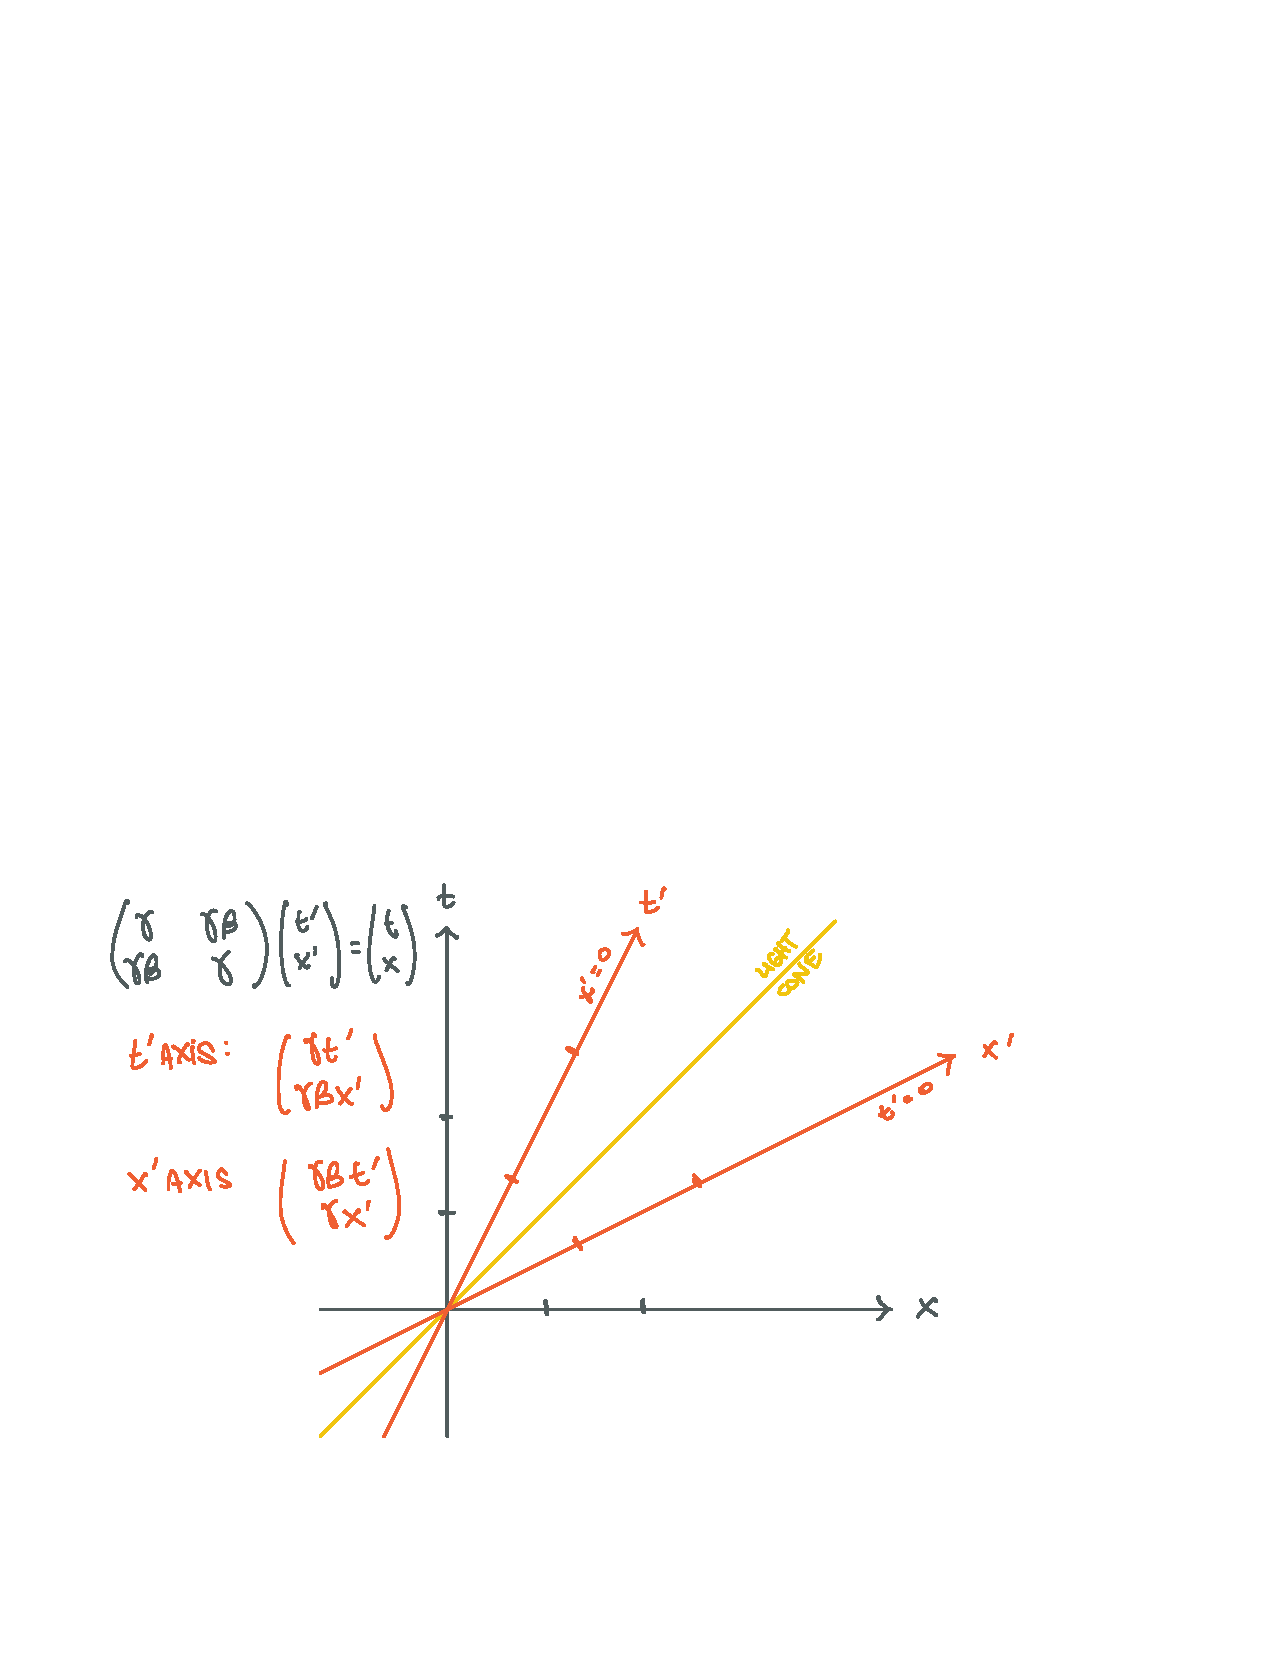
\includegraphics[width=.6\textwidth]{figures/rel_axes.pdf}
    \caption{Your coordinate system $(t,x)$ and the coordinate system of a skateboarder moving past you with velocity $\beta$. The skateboarder's coordinate system $(t',x')$ appears as the red lines in your coordinate system. The yellow line is the trajectory of light called the light cone.}
    \label{fig:re:axes}
\end{figure}

To plot the skateboarder's axes on your axis, simply recall that the $t'$ axis is determined by all points with $x'=0$. Similarly, the $x'$ axis is all points with $t'=0$. We use the Lorentz transformation to determine what these points map to:
\begin{align}
    \begin{pmatrix}
        t(t') \\ x(t')
    \end{pmatrix}
    &=
    \begin{pmatrix}
        \gamma & \gamma\beta
        \\
        \gamma\beta & \gamma
    \end{pmatrix}
    \begin{pmatrix}
        t' \\
        0
    \end{pmatrix}
    =
    \begin{pmatrix}
        \gamma t'\\ \gamma \beta x'
    \end{pmatrix} 
    \\
    \begin{pmatrix}
        t(x') \\ x(x')
    \end{pmatrix}
    &=
    \begin{pmatrix}
        \gamma & \gamma\beta
        \\
        \gamma\beta & \gamma
    \end{pmatrix}
    \begin{pmatrix}
        0 \\
        x'
    \end{pmatrix}
    =
    \begin{pmatrix}
        \gamma\beta x'\\ \gamma x'
    \end{pmatrix}
    \ .
    \label{eq:axis:transform}
\end{align}
We plot these lines in Fig~\ref{fig:re:axes}. 
We recognize that because $\gamma \geq 1$, the length of a unit tick in the $t'$ direction as seen in our reference frame has $t$-component $\gamma t' > t'$. This means that a unit step in the $t'$ direction---which we draw as a tick mark---is stretched out relative to a unit step in the $t$ direction! Of course, this is only `stretched out' because we are used to looking at plots using the Euclidean metric: the Minkowski norm remains the same. The same observation holds for a unit step in the $x'$ direction. 

We also draw a diagonal line that we label the light cone. This is the trajectory of a particle moving at the speed of light. As you increase the relative velocity $\beta$ between the two observers, the axes of one observer relative to the other approach the light cone. 
\begin{exercise}
Show that the $t'$ and $x'$ axes approach the light cone as $\beta \to \infty$. 
\end{exercise}

\subsection{Example: Muon Decay}

Cosmic rays can hit the upper atmosphere and produce muons about 10 kilometers above the surface of the Earth. These muons are highly relativistic, with a velocity of $\beta = 0.9999$. See Fig.~\ref{fig:muons}. We know from laboratory experiments that the lifetime of a muon \emph{at rest} is 2 microseconds. Based on the simple estimate $d=c\tau \approx 600$~meters, we would not expect any muons to reach the surface of the Earth. However, not only do large cosmic ray telescopes have dedicated muon detectors, but you can make your own citizen science muon detector\footnote{\url{https://muonpi.org}}. What gives?



\begin{figure}[tb]
    \centering
    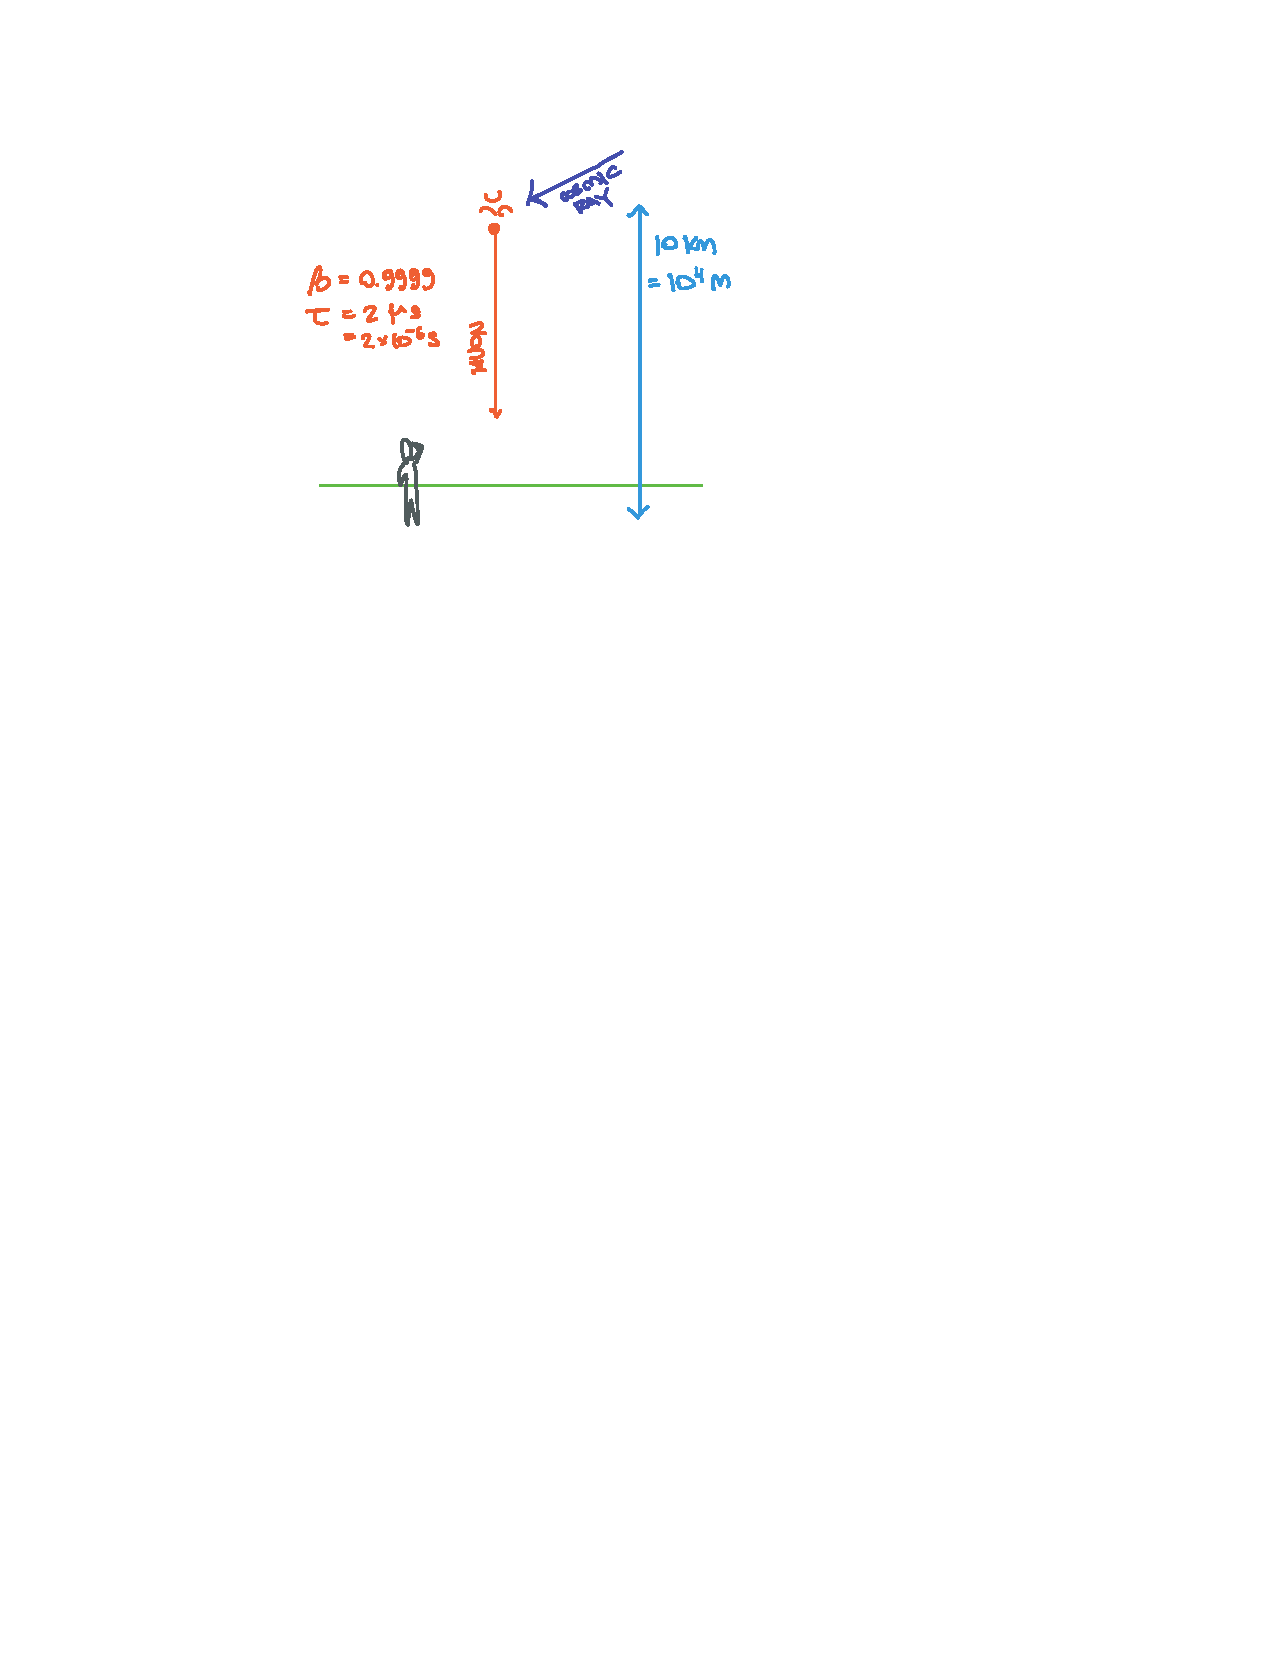
\includegraphics[width=.48\textwidth]{figures/muon.pdf}
    \caption{Very technical sketch of a muon produced in the upper atmosphere heading towards earth with velocity $\beta = 0.9999$. A stationary muon has a lifetime of $2\times10^{-6}$~seconds before it decays. The muon is produced $10^4$ meters above the surface of the earth. The speed of light is $c=3\times 10^{8}$ meters per second. If we estimate the distance traveled as $d = c\tau$, then the muon travels about $600$ meters before decaying. We would then conclude that no muons reach the surface of the earth. What's wrong with this argument?}
    \label{fig:muons}
\end{figure}

% using rotations
% time dilation picture
% length contraction picture

Here are the facts:
\begin{itemize}
    \item Both the observer on Earth and the muon agree that their relative velocity is $|\beta| = 0.9999$. 
    \item The muon's lifetime is known in the muon's rest frame. 
    \item The distance from the surface of the Earth to the upper atmosphere is known in the Earth's rest frame. 
\end{itemize}
With the understanding that boosts will mix up space and time, we can only determine the distance or time that the muon travels by calculating in the same reference frame. 


\begin{figure}[tb]
    \centering
    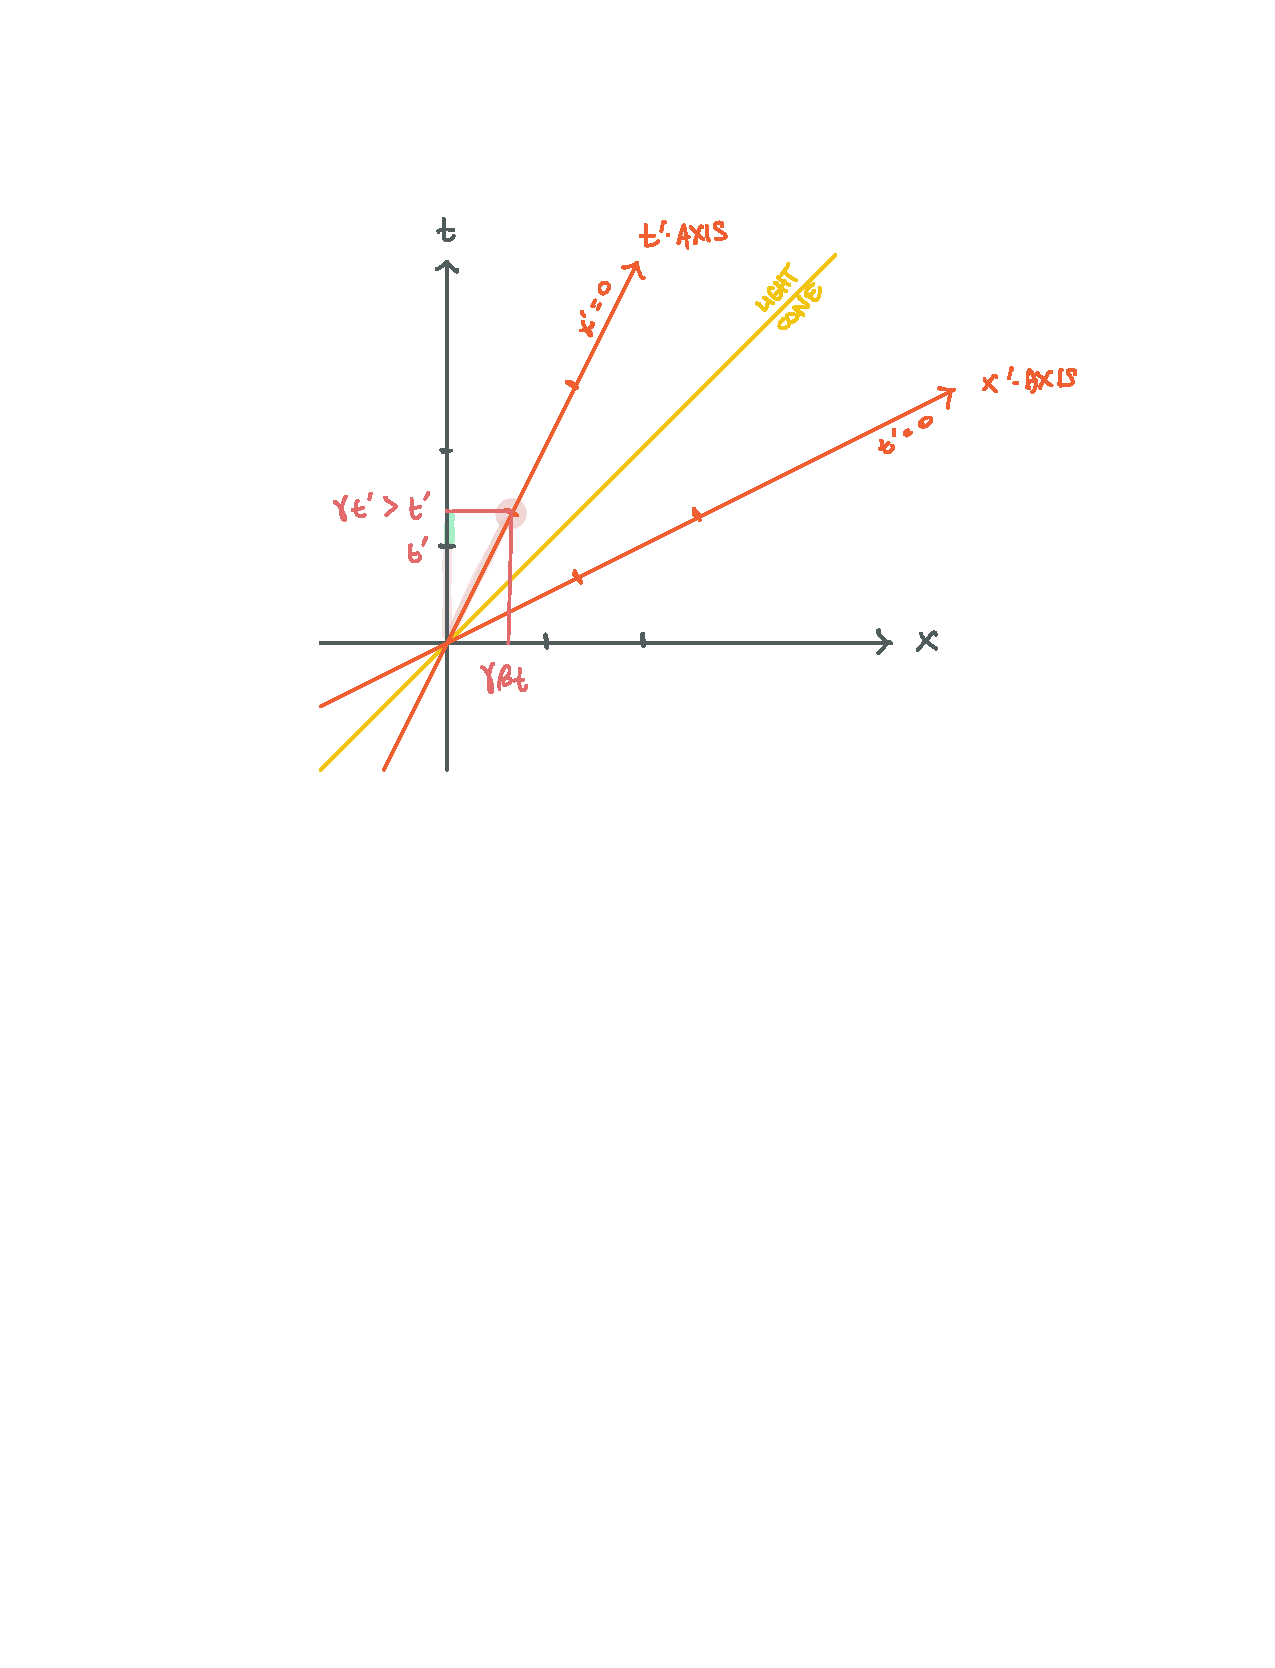
\includegraphics[width=.48\textwidth]{figures/rel_time_dil.pdf}
    \quad
    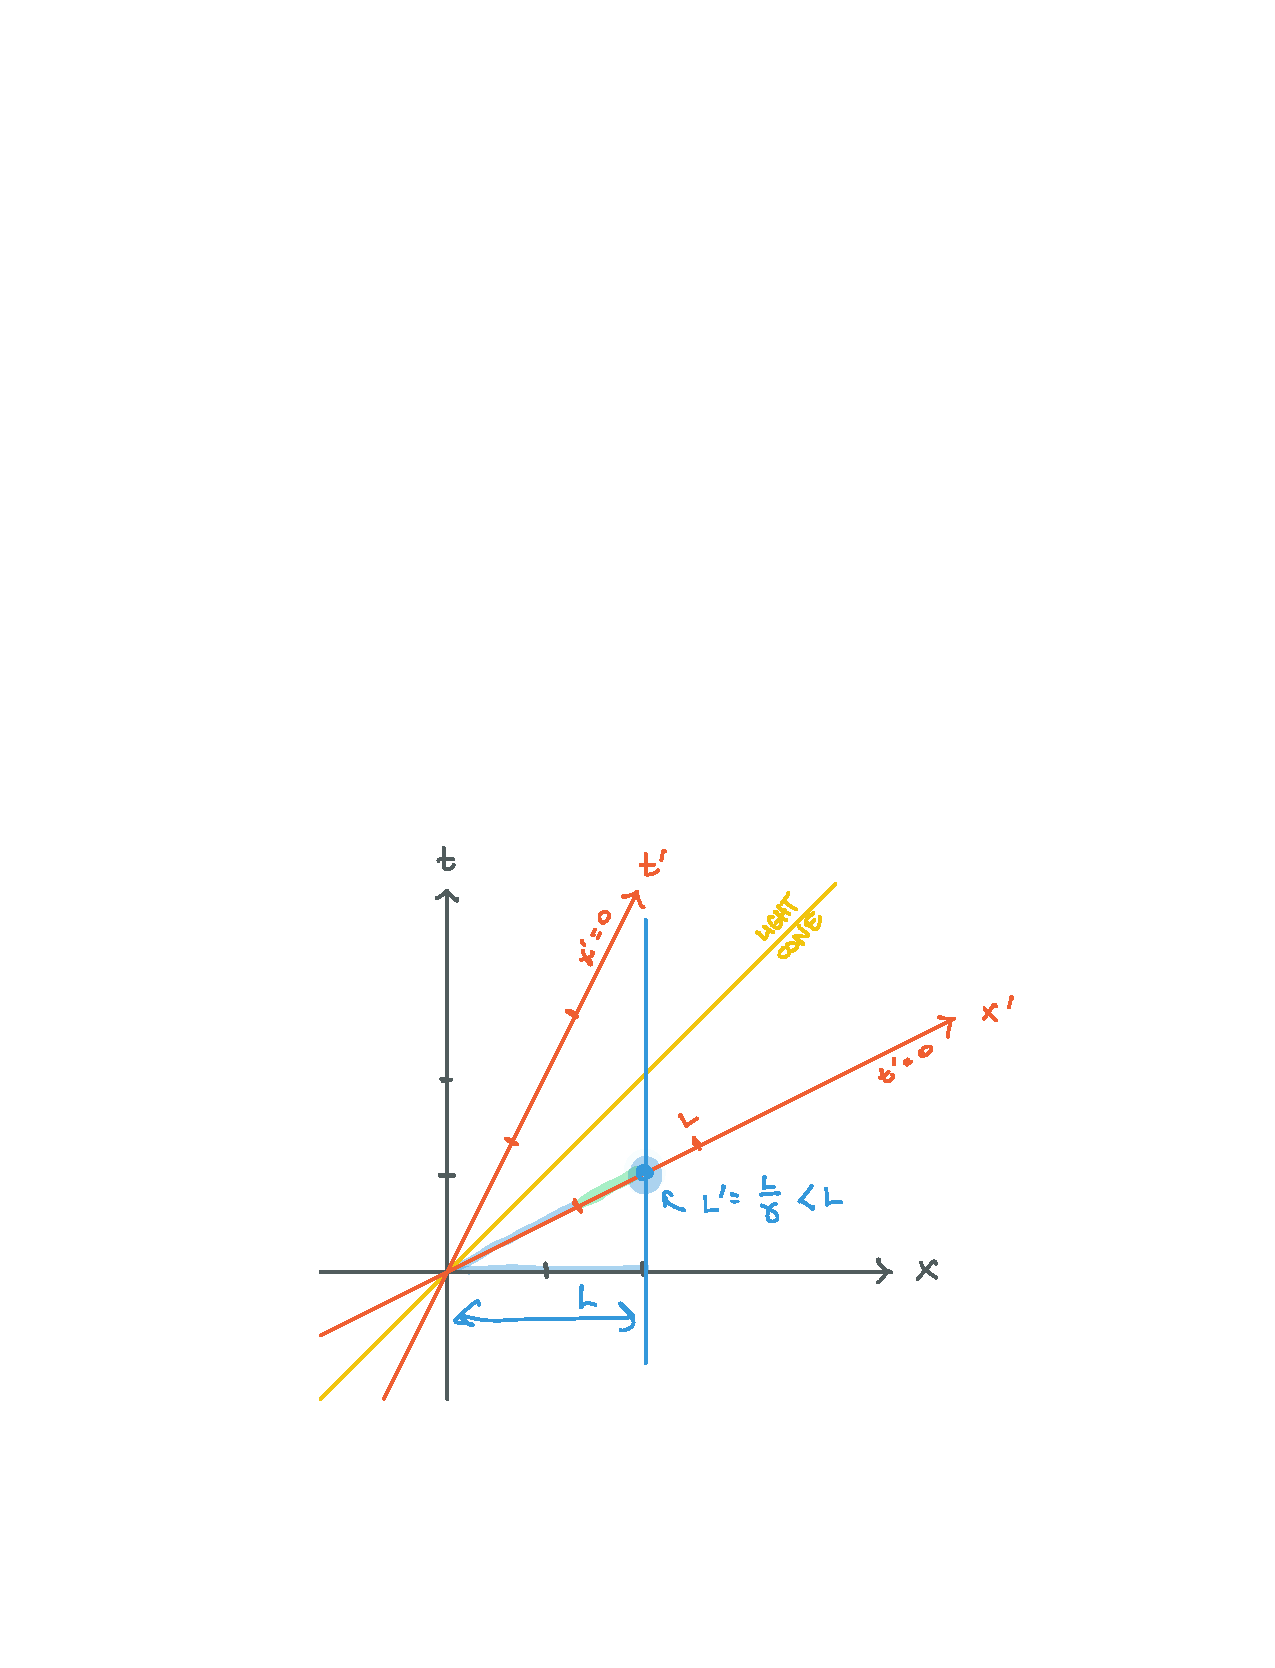
\includegraphics[width=.48\textwidth]{figures/rel_len_contractino.pdf}
    \caption{Left: the muon's lifetime is time-dilated in the Earth's frame. Right: the distance from the surface of the Earth to the upper atmosphere is length contracted in the muon's frame. }
    \label{fig:re:dilation}
\end{figure}

First let us consider calculating everything in the Earth's reference frame. This is shown on the left of Fig.~\ref{fig:re:dilation}. This means we have to take the muon's lifetime in the muon's rest frame and convert it into a lifetime in the Earth's frame. In the muon's frame the lifetime is simply 
\begin{align}
    \Delta x'^\mu &= 
    \begin{pmatrix}
    \tau \\ 0     
    \end{pmatrix} \ 
    &
    \Delta x^\mu &=
    \begin{pmatrix}
    \gamma \tau \\ \gamma\beta \tau    
    \end{pmatrix} \ ,
\end{align}
where we have noticed that the muon lifetime is a displacement along the $t'$ axis used our results in \eqref{eq:axis:transform}. We find that the lifetime in the Earth's frame is actually larger than the lifetime in the muon rest frame: $t = \gamma \tau$. There is also a spatial component, but this is no surprise: in the Earth frame the muon is moving, so when the muon decays it is in a different position. 

How much is the muon's lifetime \emph{time dilated}? We plug $\beta$ into the expression for $\gamma = (1-\beta^2)^{-1/2}$. We find\footnote{There's a cute trick here: $\beta^2 = (1-\epsilon)^2 \approx 1- 2\epsilon$ by Taylor expanding in the small number $\epsilon = 10^{-4}$.} that to one significant figure, $\gamma = 100$. This means that the time for the muon decay in the Earth's frame is $2\times 10^-4$~seconds, which means that it travels approximately $d=60~$km, which is larger than the distance from the upper atmosphere to the surface. As a sanity check: this is exactly the value in the spatial component of $\Delta x^\mu$.

Great: so one story is that relativistic muons have lifetimes that are much larger than their at-rest lifetime. This means that to the observer on earth, the muon simply lives longer than we would expect from measurements of muons at rest. There are, however, (at least) two sides to every good story. What does the muon see?

In the muon's rest frame, the muon \emph{knows} that it goes \emph{kaput} in 2~microseconds. It sees the surface of the Earth approaching it with velocity $\beta = 0.9999$. By now you can guess that must change: the measurement in the Earth's frame---that the height of the upper atmosphere is 10~km---must be different in the muon's frame. And in fact, the muon must measure the distance of the rapidly approaching Earth to be much smaller than 10~km. How does this \emph{length contraction} work? 

We show this on the right side of Fig.~\ref{fig:re:dilation}. Note that now we have a measurement in the Earth frame (a vertical line denoting a fixed distance) that we want to project onto the muon frame (red axes). In the Earth frame, we denote the distance by two unit ticks in the spatial direction. In the muon frame, this line intersects the $x'$ axis with \emph{less} than two ticks.

\begin{exercise}
Using the Lorentz transformation laws, show that the distance from the muon to the surface of the Earth at the moment of the muon's creation is $L'=L/\gamma$ where $L=10$~km is the distance in the Earth frame. 
\end{exercise}

\begin{exercise}
Rephrase everything in this example in terms of the isometries of Minkowski space. 
\end{exercise}

\subsection{Example: What does someone else measure?}
\label{sec:relativity:alien}
% using inner products
% contrast to boosting

Momentum is also a four-vector in relativity. The components of the momentum four vector are in \eqref{eq:momentum:4vec}, which we write succinctly as
\begin{align}
    p^\mu = 
    \begin{pmatrix}
        E \\ \vec{p}
    \end{pmatrix} \ .
\end{align}
If we measure the four-momentum of a particle in our laboratory, then we know that the energy of the particle is $p^0 = E$. That's by definition of what the first component of the four-momentum is---we did not actually do any work to do that. 

In special relativity there is another object called the four-velocity. In our rest frame, our four velocity is
\begin{align}
    v^\mu = \begin{pmatrix}
        1\\ 0
    \end{pmatrix} \ .
    \label{eq:4:velocity:in:rest:Frame}
\end{align}
This literally means that when we are at rest, we are moving one second per second in the time direction. Objects moving relative to us have four velocities that are Lorentz transformations of the $v^\mu$ above. 

We notice that we can write the energy of a particle in a way that uses the inner product:
\begin{align}
    \langle v, p\rangle = p\cdot v = g_{\mu\nu} p^\mu v^\nu \ .
\end{align}
Of course, all this does is pick out the $p^0$ component, as we knew it had to. However, unlike writing $p^0$, the inner product $p\cdot v$ has no indices. It is a pure number and so it does not transform under Lorentz transformations. 

At this point you wonder if we are simply reciting random facts that we have developed. Consider the following scenario illustrated in Fig.~\ref{fig:alien}.
% 
\begin{figure}[tb]
    \centering
    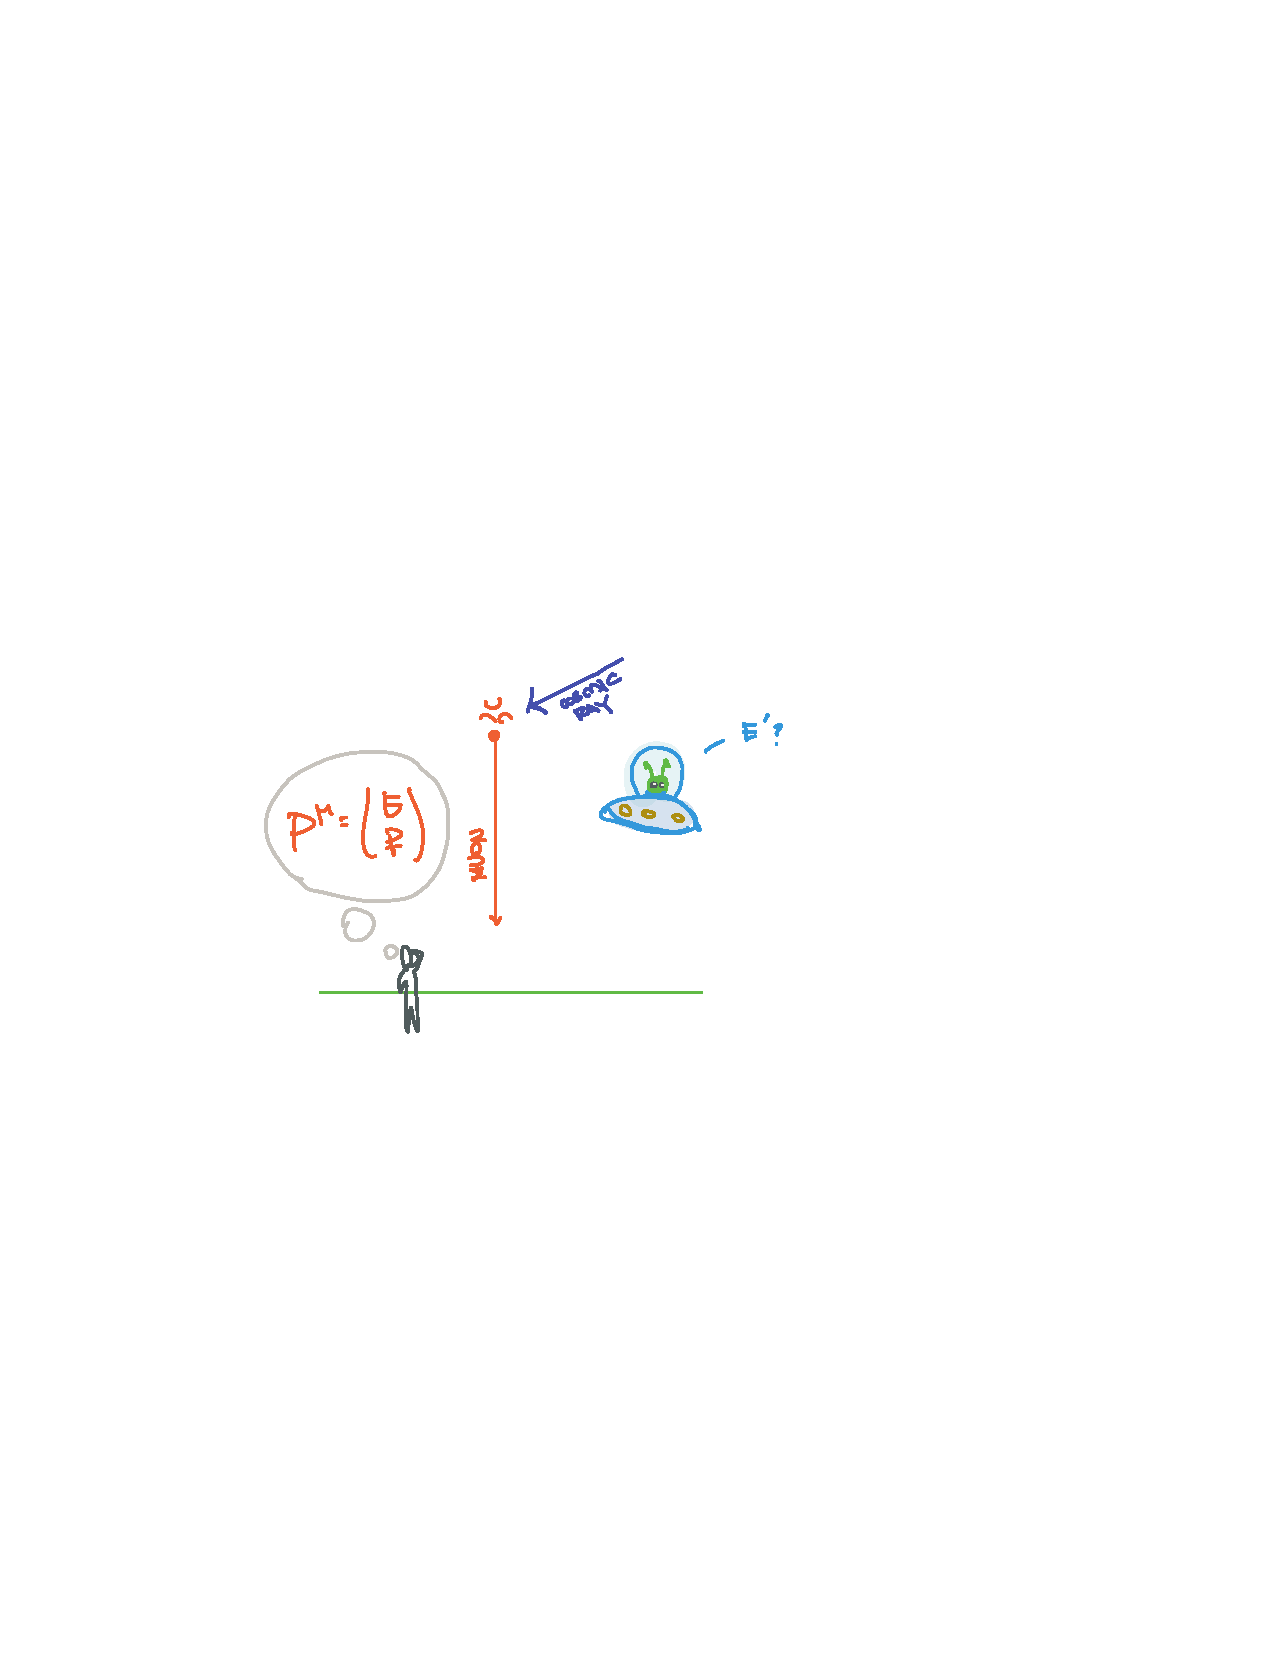
\includegraphics[width=.5\textwidth]{figures/alien.pdf}
    \caption{You measure the four-momentum of a particle. One of the components is the energy of the particle. What is the energy that an alien moving at some velocity $\beta$ relative to you measures?}
    \label{fig:alien}
\end{figure}
% 
While you have measured the energy $E$ of a particle, you notice an alien traveling relativistically with velocity $\beta$ relative to you. The alien has sophisticated equipment to measure the particle energy, and you know that the alien measures a different energy $E'$ relative to what you measure. How can you determine what that energy is?

One way to do this is to calculate the full Lorentz transformation between your frame and the alien frame. It turns out, however, that we can use the four-velocity as a useful trick. All objects with mass have a four-velocity equal to \eqref{eq:4:velocity:in:rest:Frame} in their rest frame. This means that the alien measures the particle to have energy $v_\text{alien}\cdot p_\text{alien}$, where the subscript `alien' means that these are all calculated in the alien's frame.

We now remember that $v_\text{alien}\cdot p_\text{alien}$ is a number. It does not matter what frame we calculate it in. Thus it is equivalent to the same dot product measured in our frame:
\begin{align}
E'=
    v_\text{alien}\cdot p_\text{alien} = v\cdot p \ ,
\end{align}
where the right-hand side is the alien four-velocity and the particle four-momentum as measured in our frame. The alien four-velocity is simply a Lorentz transformation of \eqref{eq:4:velocity:in:rest:Frame}. More practically, it is something that you can measure in your own frame. 


\begin{exercise}
Rephrase everything in this example in terms of the inner product in Minkowski space. Bonus if you use the word `projection.'
\end{exercise}


% index, bolfcaced, metric signature
% natural units... because vectors and energies


\subsection{Example: the electromagnetic field stength}
% motivate this from the unification of magnetism and electricity
% transformation laws

\begin{figure}[tb]
    \centering
    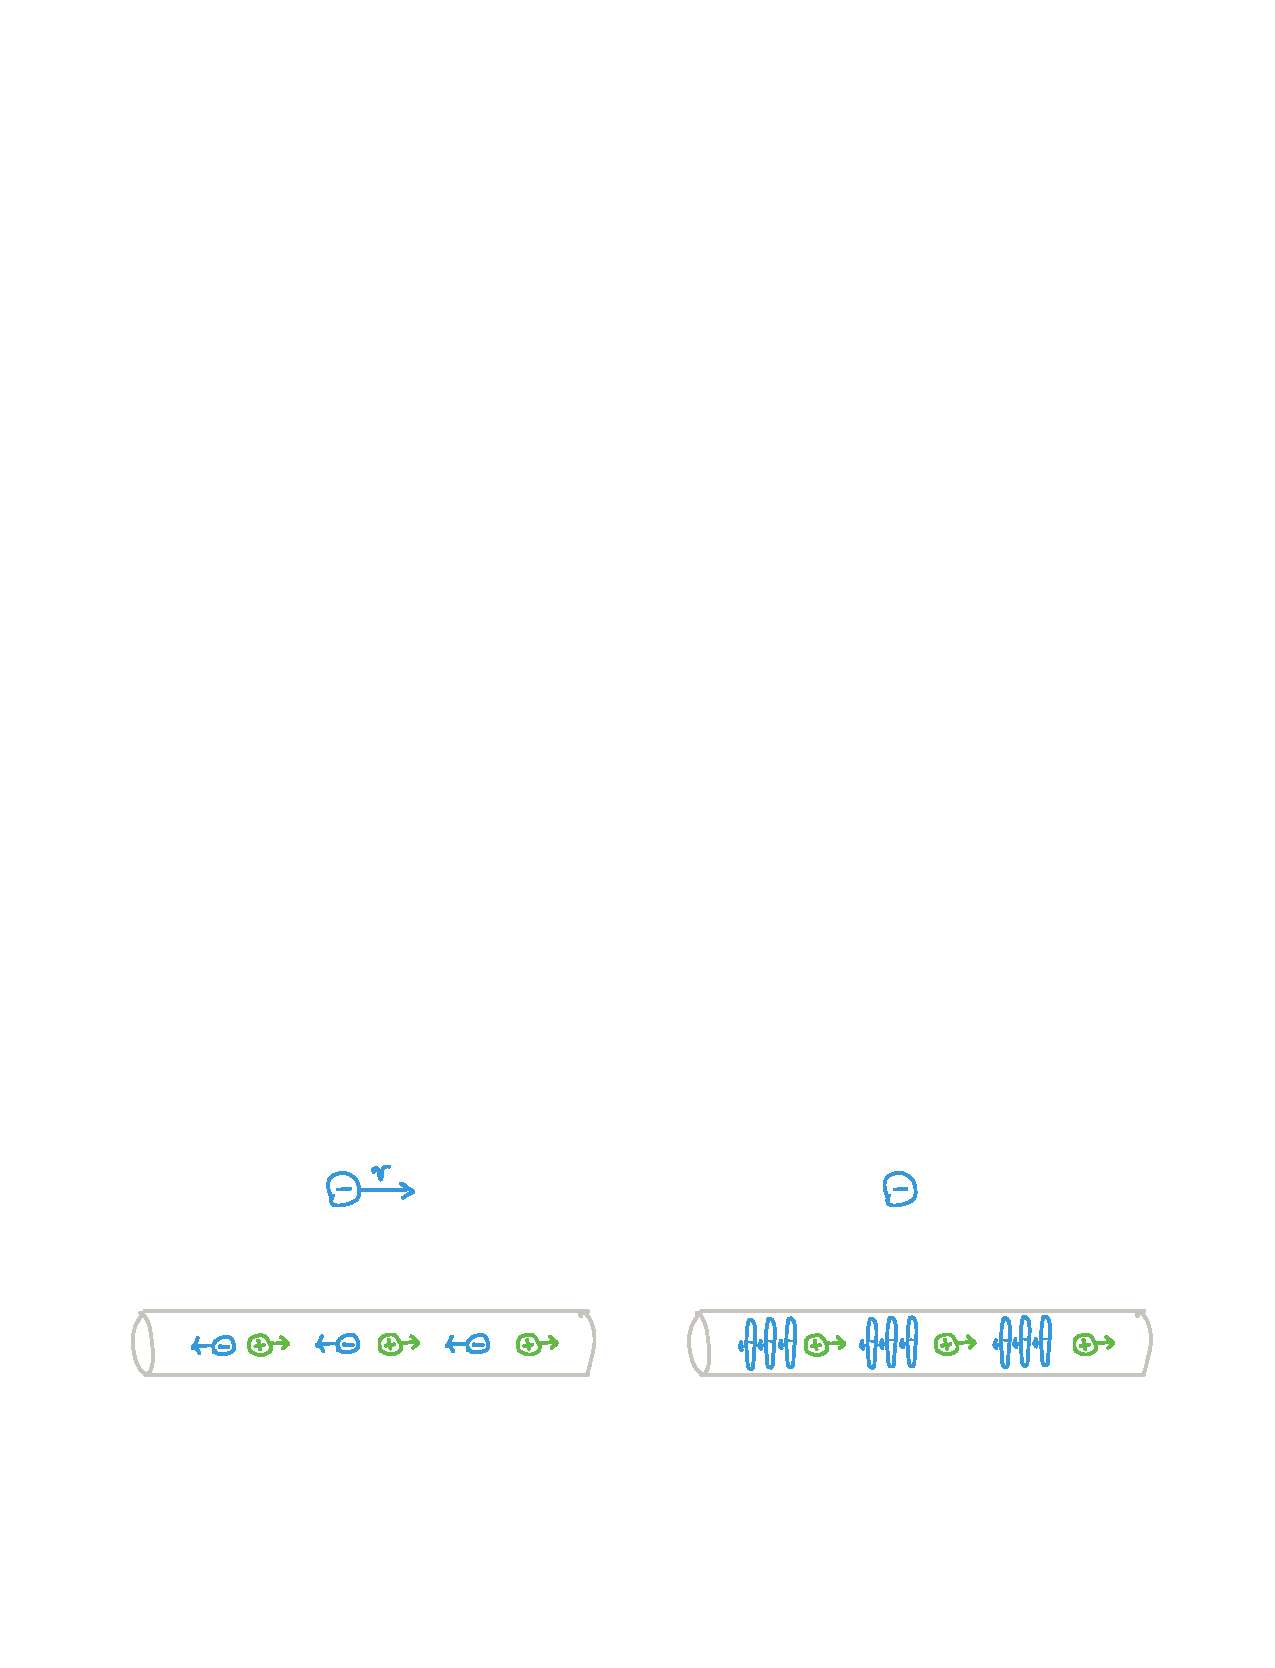
\includegraphics[width=.8\textwidth]{figures/EMcurrent.pdf}
    \caption{Left: an electron moves near a current. The current has no net electric charge. In the absence of magnetism, we expect the electron to move in a straight line. Right: if we boost into the electron frame, the particles in the current moving in the opposite direction are length-contracted. This means that the charge density increases. The stationary electron now feels a net electric force. This implies that something is missing in the picture on the left.}
    \label{fig:current}
\end{figure}

Another place where special relativity rears its head is in electrodynamics. Electricity and magnetism are two manifestations of the same electromagnetic phenomenon. This is illustrated in Fig.~\ref{fig:current}. If you did not know about magnetism, you would find a paradox when you consider a charged particle moving along a current. In one frame, the current is an equal number of positive and negative charges moving in opposite directions.\footnote{I suppose more realistically the negative charges move while the positive charges stay put---that does not change the conclusion.} If you boost to the external charged particle's rest frame, length contraction forces one species of the current particles to increase their charge density relative to the other species. This creates a net electric field that acts on the stationary external particle. Without magnetism, the first frame is missing this additional force. 

The electric and magnetic fields are unified in the \emph{electromagnetic field strength}, which is a two-index tensor:
\begin{align}
    F^{\mu\nu}
    &=
    \begin{pmatrix}
        0&-E^x&-E^y&-E^z\\
        E^x&0&-B^z&B^y\\
        E^y&B^z&0&-B_x\\
        E^z&-B^y&B^x&0
    \end{pmatrix} \ .
    &
    F_{\mu\nu}
    &=
    \begin{pmatrix}
        0&E^x&E^y&E^z\\
        -E^x&0&-B^z&B^y\\
        -E^y&B^z&0&-B_x\\
        -E^z&-B^y&B^x&0
    \end{pmatrix} \ .
\end{align}
We see that electricity and magnetism are unified in that their components mix into one another under a Lorentz transformation. 
\begin{exercise}
Confirm that $F_{\mu\nu} =g_{\mu \alpha}g_{\nu\beta} F^{\alpha\beta}$ with the (3+1)-dimensional Minkowski metric $g_{\mu\nu}$. 
\end{exercise}
\begin{exercise}
Find the components of $F'^{\mu\nu}$ under a boost along the $z$-direction. 
\end{exercise}


\section{Central Dogmas}

We interrupt our regularly scheduled broadcasting\footnote{This is a phrase from my childhood. Television stations would interrupt an ongoing show to present `breaking news' that they felt all of their viewers needed to see.} to take stock of the ``big picture'' that we are slowly developing. In this section, we review the salient lessons from the first part of this course and present some ``practical perspectives'' on how to think about the machinery developed. We close by introducing the idea of eigenvectors and eigenvalues.

\subsection{Vectors are not columns}
% also: vectors are not components, but they're convenient

Vectors are not columns of numbers. The numbers are the \emph{components} of a vector: we write these with indices. The components just tell you how to write the vector as a linear combination of basis vectors:
\begin{align}
    \ket{v} = v^i \ket{i} = v^i \bas{e}_i \ .
\end{align}
All of the `meaning' of the vector is encoded in the basis vectors.
In fact, we have \emph{deliberately} avoid stating what a vector `means.' This meaning is abstract because we want it to be general. Maybe your basis vectors are possible velocities of a particle at a point in space. Maybe the basis vectors are units of something you are counting. Maybe the basis vectors are Fibonacci sequences, or the primary colors. The point is that each of these very different vector spaces are described by the same basic machinery. The vectors live in a vector space, $V$, which carries this abstraction. 

If we generalize this a bit: if you have done a bit of programming\footnote{In this century, \emph{every} physicist should be able to program.}, then you may wonder how a tensor is different from an array. An array is a (hyper-)grid of numbers. These are what are encoded by the components of a tensor, say $T\aij{ij}{k}$. However, a tensor is more than that: it comes with a transformation law for how these components change under an isometry (rotation) that lets us say ``an observer in a different basis would measure the components of the tensor to be $(T')\aij{ij}{k}$.


\subsection{Everything is a vector space, everything is a linear map}

We adopt the convention where vectors have upper indices. This allowed us to introduce row vectors as funny objects with lower indices. We then saw that these two objects are dual to each other: 
\begin{enumerate}
    \item The row vectors are linear functions of the column vectors.
    \item The column vectors are linear functions of the row vectors.
\end{enumerate}
In both cases, they are linear functions that output numbers. We called the vector space of row vectors the dual space, $V^*$. The above statements are:
\begin{enumerate}
    \item Row vector, $\row{w}:\;V\to \RR$
    \item Column vector, $\vec{v}:\;V^*\to \RR$
\end{enumerate}

We then realized that we could have linear functions that go from tensor products of vector spaces. That is, linear functions that take some number of row vectors and some number of column vectors and return a number. A tensor with $p$ upper indices (vector-like indices) and $q$ lower indices (row-vector like indices) is a linear map that takes in $p$ row vectors and $q$ column vectors to output a number. In this point of view, tensors are simply linear transformations. 

\subsection{What the inner product brings}

The inner product is a special function that takes two vectors and spits out a number. We may thus write it as a tensor with two lower indices; this tensor is called the metric. A \textbf{metric space} or equivalently \textbf{inner product space} is a vector space with a metric. The metric and its inverse allow us to raise and lower indices. This gives us a way to create row vectors from column vectors. 

We identified a set of linear transformations from $V\to V$ that leave the metric invariant. These are called \textbf{isometries}. Under an isometry, $g'_{ij} = g_{ij}$. Isometries are generalizations of rotations: under an isometry, an orthonormal basis is transformed into another orthonormal basis. From a physics perspective, an isometry takes us from one reference frame to another. That is: a physical quantity may be tensorial. The components of the tensor has significance to a particular observer with a particular basis. A different observer has a different basis that are related to the first basis by an isometry. By performing this transformation, we can determine what the second observer measures.

It also afforded us a notion of the \textbf{adjoint} of a matrix, $A^\dag$ which we define using the inner product:
\begin{align}
    \la A \vec{v}, \vec{w} \ra 
    \equiv
    \la \vec{v}, A^\dag\vec{w} \ra  \ .
\end{align}
The adjoint may seem like a curiosity, except that it defines our notion of a \emph{nice} matrix. A \emph{nice} matrix is one that is self-adjoint: $A^\dag = A$. From the above definition, we show that the adjoint is equivalent to the Hermitian conjugate: 
\begin{align}
    (A^\dag)\aij{i}{j} = g_{aj}(A\aij{a}{b})^*g^{bi} \ ,
\end{align}
that is: the transpose with a complex conjugate. We call self-adjoint matrices \textbf{Hermitian}. This is the generalization of a symmetric matrix. These matrices are nice because they can be diagonalized by an isometry, and the basis in which they are diagonal will be so convenient that we devote all of Section~\ref{sec:eigensystem} to it.

\subsection{Basis Dependence}

When we write the components of a tensor, we assume some basis. In the `high school' picture of vectors as columns of numbers, this basis takes the form
\begin{align}
    \bas{e}_1 &= 
    \begin{pmatrix}
        1 \\ 0 \\ \vdots \\ 0
    \end{pmatrix}
    &
    \bas{e}_2 &= 
    \begin{pmatrix}
        0 \\ 1 \\ \vdots \\ 0
    \end{pmatrix}
    & \cdots &
    &
    \bas{e}_N &= 
    \begin{pmatrix}
        0 \\ 0 \\ \vdots \\ 1
    \end{pmatrix} \ .
\end{align}
We colloquially call this the \textbf{standard basis}.
However, there is nothing holy about this basis. It just happens to be the basis of one observer. The underlying physics of the system described by tensors is \emph{basis independent}. Mathematicians address this by eschewing bases whenever they can. Often this means that physicists reading a mathematics textbook will be amazed at (1) how clean their equations look and (2) how incomprehensible those equations are when you want to figure out what they look like to a specific observer. 

Nature is basis-independent. Sometimes we can be sneaky about this: we can derive a result in a particular basis, then write that same result in a way that is basis-independent\footnote{For example: write the final result in a way where all indices are contracted.} so that the basis-independent result is true in any basis. We demonstrated this approach in special relativity in Section~\ref{sec:relativity:alien}. 

In what follows, we will contrast the ``standard basis'' with other convenient bases that come up. In particular, we will be especially fond of the \emph{eigenbasis} where a given (Hermitian) matrix is diagonal. The general strategy we follow will be to 
\begin{enumerate}
    \item We have a matrix $M$ in the standard basis. 
    \item We find a special basis (eigenbasis) where $M$ takes a convenient form. We rotate to this convenient basis.
    \item In the convenient basis, we do whatever manipulations we need to do to solve our problem. Maybe we need to take an inverse. Maybe it is an exponential. Whatever it is, this is the step where we ``do the physically significant'' mathematical step.
    \item The result that we get is not always easy to interpret. So we have to rotate back to the standard basis. This gives a full solution to our problem in the basis that the problem was originally posed.
\end{enumerate}






\subsection{A multitude of conventions}

It is potentially confusing that physicists use multiple conventions to describe what are essentially the same ideas in linear algebra. Table~\ref{table:vectors:numbers} makes some of these connections explicit.

\begin{table}
    \renewcommand{\arraystretch}{1.3} % spacing between rows
    \centering
    \begin{tabular}{ @{} llll @{} } \toprule % @{} removes space
        Vector Space & $\RR$ & $\CC$ & $\infty$-dimensional
        \\ \hline
        Vector/ket 
            & $\vec{v} = \ket{v}$ 
            & $\vec{v} = \ket{v}$
            & $f$
            \\
        Basis vector
            & $\bas{e}_i = \ket{i}$ 
            & $\bas{e}_i = \ket{i}$ 
            & $\hat{e}_i(x)$
            \\
            & 
            & 
            & $\hat{e}_p(x)$
            \\
        Components
            & $v^i \in \RR$
            & $v^i \in \CC$
            & $f^i, \tilde{f}(p) \in \CC$
            \\
        % Components
            & $\vec{v} = v^i\bas{e}_i = v^i\ket{i}$
            & $\vec{v} = v^i\bas{e}_i = v^i\ket{i}$
            & $f(x) = f^i\, \hat{e}_i(x) $
            \\
            & 
            & 
            & $f(x) = \int \dbar p\,\tilde f(p) e_p(x)$
        \\
        Row vector/bra
            & $\row{w} = w_i\rbas{e}^i = w_i\bra{i}$
            & $\row{w} = w_i\rbas{e}^i = w_i\bra{i}$
            & distribution, e.g.~$\delta(x)$
        \\
        Matrix
            & $A = A\aij{i}{j}\ket{i}\bra{j}$
            & $A = A\aij{i}{j}\ket{i}\bra{j}$
            & operator, e.g.~$\frac{d^2}{dx^2}$
        \\
        Inner Product
            & $\la v, w \ra = g_{ij}v^iw^j$
            & $\la v, w \ra$
            & $\la f, g \ra = \int dx\, f^*(x)g(x)$        
            \\
        % Inner Product
            & $\la v, w \ra = \la w,v\ra$
            & $\la v, w \ra = \la w,v\ra^*$
            & $\la f, g \ra = \la g,f\ra^*$
        \\
        Adjoint
            & Transpose
            & Hermitian Conjugate
            & Integration by parts
        \\
        % Adjoint
            & $(A^T)\aij{i}{j} = g_{jk}A\aij{k}{\ell}g^{\ell i}$
            & $(A^\dag)\aij{i}{j}= [(A^T)\aij{i}{j}]^*$
            & e.g.~$(d/dx)^\dag = -(d/dx)$
        \\
        Self-adjoint
            & Symmetric
            & Hermitian
            & Sturm--Liouville
        \\
        % Self-adjoint
            & $A^T = A$
            & $A^\dag = A$
            & $\mathcal O^\dag = \mathcal O$
        \\
        % Self-adjoint
            & $\RR$ Eigenvalues
            & $\RR$ Eigenvalues
            & $\RR$ Eigenvalues
        \\
        % Self-adjoint
            & $\perp$ Eigenvectors
            & $\perp$ Eigenvectors
            & $\perp$ Eigenvectors
        \\
        Isometry, e.g.
            & Rotations, Boosts
            & Unitary Matrices
            & Change of variable
        \\ \bottomrule
    \end{tabular}
    \caption{
        Terms and notation in real, complex, and infinite-dimensional vector spaces. 
        \label{table:vectors:numbers}
  }
\end{table}

\subsection{The un-mathematical idea of niceness}
\label{sec:nice}

Mathematicians like generality. If there is a true statement for a class of matrices, they are not content with stating the truth---they want to either extend it to all matrices, or otherwise clearly articulate every necessary assumption. This is sometimes caricatured as an obsession with marginal cases. Physicists have the luxury of not having to worry about that: our matrices are all typically ``nice.'' In this section, we try to give a definition for what \emph{nice} means. 

\paragraph{Gold tier} The nicest matrices are multiples of the identity matrix, $\one$. These matrices are diagonal. If you rotate them, they don't change. The inverse of these matrices is simply the inverse of the coefficient, $(\alpha \one)^{-1} = \alpha^{-1} \one$. These matrices turn out to be \emph{too} nice. The matrix is proportional to the identity no matter what basis you are in.

\begin{exercise}
Show that if $M = \alpha \one$, then the rotation of $M$ is still $M$:
\begin{align}
    RMR^\dag = M \ .
\end{align}
\end{exercise}

\paragraph{Silver tier} The next-nicest matrices are diagonal matrices
\begin{align}
\hat M = 
    \begin{pmatrix}
        \lambda_1 & & & \\
         & \lambda_2 & & \\
         & & \ddots & \\
         & & & \lambda_N
    \end{pmatrix} \ .
    \label{eq:diagonal:matrix}
\end{align}
Diagonal matrices are a sign that you are using the \emph{right} basis. When acting on the $i^\text{th}$ basis vector, we simply pick up $\lambda_i$:
\begin{align}
    \hat M \ket{i} = \lambda_i \ket{i} \ .
\end{align}
This pattern is so nice that we call this basis an \emph{eigenbasis}. The diagonal element $\lambda_i$ is called an \emph{eigenvalue} and the corresponding basis element $\ket{i}$ is called an \emph{eigenvector}. We will specifically be interested in the case where all of the eigenvectors $\lambda_i$ are real, even when we are in a complex vector space. Another nice feature of diagonal matrices is that their inverse is easy:
\begin{align}
    \hat M = 
        \begin{pmatrix}
        \lambda_1^{-1} & & & \\
         & \lambda_2^{-1} & & \\
         & & \ddots & \\
         & & & \lambda_N^{-1}
    \end{pmatrix} \ .
\end{align}


\begin{exercise}
Show that if $\hat M$ is a diagonal matrix \eqref{eq:diagonal:matrix}, then we can make sense of the exponential of this matrix by generalizing the Taylor expansion of the exponential:
\begin{align}
e^{\hat M} = 
    \begin{pmatrix}
        e^{\lambda_1} & & & \\
         & e^{\lambda_2} & & \\
         & & \ddots & \\
         & & & e^{\lambda_N}
    \end{pmatrix} \ .
    \label{eq:diagonal:matrix:exponential}
\end{align}
Argue that you can also take the logarithm of a diagonal matrix. 
\end{exercise}


\begin{exercise}
Show that if $\hat M$ is a diagonal matrix then the following identity holds:
\begin{align}
\Tr \ln \hat M = \ln \det \hat M
\label{eq:tr:log:M:eq:ln:det:M:diag}
\end{align}
This relation turns out to be true even if we replace $\hat M$ by a matrix that is not diagonal.
\end{exercise}



\paragraph{Bronze tier} Self-adjoint (Hermitian) are matrices that that can be diagonalized. This means that we can alternatively define them to be rotations of diagonal matrices\footnote{For complex matrices, replace `rotation' with the appropriate isometry. This is usually a unitary matrix, $U$, that satisfies $U^\dag U = \one$.}:
\begin{align}
    M = R \hat M R^\dag \ .
\end{align}
Self-adjoint matrices have some nice features that we will exploit in Section~\ref{sec:eigensystem}. Most of the matrices of physical significance are Hermitian. That also means that physicists spend a lot of time \emph{diagonalizing} Hermitian matrices to find the right basis where they are diagonal. As a caveat, we will usually assume that the eigenvalues are all non-zero.\footnote{A zero eigenvalue means that the matrix is not invertible. This is most clearly seen tn the basis where the matrix is diagonal.}


\paragraph{Isometries} Isometries are a totally different class of matrices. Isometries are linear transformations that preserve the metric. This means that they transform orthonormal bases into other orthonormal bases. When we diagonalize a Hermitian matrix, we use the isometries of our metric space to change basis. In this sense, we should think about isometries as a transformation between basis vectors. 

\paragraph{Projections} Projections are \emph{not nice} matrices, except when they are useful. Most \emph{non-invertible} matrices are projections. They are non-invertible because they throw out information. A true projection would be a matrix $\ket{\hat{v}}\bra{\hat{v}}$ that acts on a vector by singling out the component along a particular direction. We thus remove projections from our definition of a `nice' matrix. Nice matrices are invertible. Of course, projections can be useful---so we single them out here as a second special class of linear transformation.

\paragraph{Trash} What about all the other kinds of matrices? All of our matrices are assumed to be square. These square matrices may be infinite dimensional, but the are square. The uses of non-square matrices are few and far between. Matrices that are not Hermitian, isometries, or projections are also rare. 

\vspace{1em}

In this course and in our physics lives, we almost exclusively focus on the \emph{nice} matrices acting on \emph{nice} metric spaces. 

% one, diagonal, rotations, projections, worse

% \subsection{The eigensystem}

\section{Eigensystem}
\label{sec:eigensystem}

The German prefix \emph{eigen-} means ``proper.'' The sense in which this is proper is analogous to our notion of niceness in Section~\ref{sec:nice}. Consider the following expression for a matrix $M$:
\begin{align}
    M\ket{\xi} = \lambda\ket{\xi} \ .
\end{align}
Here $M$ is a matrix and $\lambda$ is a number. We say that this is an eigenvalue equation because $M$ acts on a particular vector, $\ket{\xi}$, and the result is a rescaling of that vector, $\lambda\ket{\xi}$. The vector $\ket{\xi}$ is called an \textbf{eigenvector} of $M$ with \textbf{eigenvalue} $\lambda$.  The matrix $M$ acts on the eigenvector $\ket{\xi}$ the way that a diagonal matrix acts on a basis vector.
 
\begin{exercise}
Show that if $\ket{\xi}$ is an eigenvector of $M$ with eigenvalue $\lambda$, then it is also an eigenvector of $M\inv$ with eigenvalue $\lambda\inv$. 
\end{exercise}

\subsection{Self Adjoint (Hermitian) Matrices}

The eigenvalue problem for Hermitian (self-adjoint) matrices is particularly compelling. The following two facts show why:
\begin{enumerate}
    \item The eigenvalues of Hermitian matrices are real.
    \item The eigenvectors of Hermitian matrices are orthogonal.
\end{enumerate}

\begin{exercise}
Prove the above statements. 
\end{exercise}

\begin{exercise}\label{ex:orthogonal:eigenvectors:not:normal}
We say that the eigenvectors of Hermitian matrices are \emph{orthogonal}, but not necessarily orthonormal. This is because the eigenvalue condition does not guarantee a normalization of the eigenvector. Show that if $\ket{\xi}$ is an eigenvector of $M$ with eigenvalue $\lambda$, then $\alpha\ket{\xi}$ is also an eigenvector of $M$ with eigenvalue $\lambda$. In the same vein, argue that we can always \emph{choose} eigenvectors that are normalized so that the eigenvectors of a Hermitian matrices can be chosen to be an orthonormal basis.
\end{exercise}

\subsection{Finding Eigenvalues: Characteristic Equation}

Suppose you have a Hermitian matrix $M$. This means that there is a nice basis where $M$ is diagonal, which we indicate with a hat: $\hat M$. In this \emph{eigenbasis}, each basis vector $\ket{\xi_i}$ has an associated eigenvalue $\lambda_i$. Suppose that none of the eigenvalues are zero so that $\hat M$ is nice and invertible. The diagonal elements of $\hat M$ are simply these eigenvalues, see \eqref{eq:diagonal:matrix}. This means that the matrix $\hat M - \lambda_i \one$ is diagonal with (at least) one zero element: the the $i^\text{th}$ element along the diagonal:
\begin{align}
\hat M -\lambda_i\one = 
    \begin{pmatrix}
        (\lambda_1 - \lambda_i) & & & && \\
         & (\lambda_2 - \lambda_i) & & && \\
         & & \ddots &&& \\
         & & & 0 & & \\
         & & && \ddots & \\
         & & &&& (\lambda_N-\lambda_i)
    \end{pmatrix} \ .
    \label{eq:characteristic:1}
\end{align} 
We can exploit this curious fact using the observation in Example~\ref{eg:determinant:of:diagonal}: the determinant of a diagonal matrix is simply the product of its diagonal elements. This means that
\begin{align}
     \det(\hat M - \lambda \one) = 0
     \label{eq:characteristic:2}
\end{align}
whenever $\lambda$ is an eigenvalue of $\hat M$. This would be a great way to find the eigenvalues of diagonal matrix, $\hat M$, if it weren't for the fact that this is a silly task: if $\hat M$ is diagonal, then you can simply \emph{read off} the eigenvalues from the diagonal elements. It would be \emph{much} more useful if we had an expression like \eqref{eq:characteristic:2} that we could use to find the eigenvalues of non-diagonal matrices.  

It turns out that we can do this. Recall \eqref{eq:det:of:product}: the determinant of a product of matrices is the product of the determinants. We motivated this from the observation that the determinant is the area of a parallelogram in two dimensions---though the result generalizes hyper-volumes of \emph{parallelpipeds} in any number of dimensions. From this observation, we also found that the determinant of an inverse matrix is the inverse of the determinant \eqref{eq:det:of:inverse}. This means that
\begin{align}
    \det(R\hat M R^\dag) = 
    \det R \; \det \hat M \; \det R^\dag
    =
    \det R \; \det \hat M \; \frac{1}{\det R}
    =
    \det \hat M \ .
\end{align}
Here we used the fact that the adjoint of a rotation\footnote{And again, this generalizes to complex matrices with a Euclidean metric to a unitary matrix. In full generality, this is an isometry.} is its inverse. Using the fact that $R\one R^\dag = \one$, we may thus rotate \eqref{eq:characteristic:2} to a basis where $\hat M$ is not diagonal:
\begin{align}
     0=\det(\hat M - \lambda \one) 
     = \det\left[R(\hat M - \lambda \one)R^\dag\right]
     = \det(R\hat M R^\dag - \lambda \one) 
     = \det(M - \lambda \one) 
     \label{eq:characteristic:equation} \ .
\end{align}
This is the \textbf{characteristic equation} for the eigenvalues of $M$. This is incredibly powerful: suppose you have a nice, invertible, self-adjoint matrix $M$. The matrix is not diagonal and so it is not obvious what its eigenvalues are. The characteristic equation gives you a polynomial in $\lambda$ that you can solve to determine the values of $\lambda$ that are eigenvalues of $M$. For an $N$-dimensional vector space, you will have an $N$-dimensional polynomial. Because the matrix is self-adjoint, we know that the eigenvalues are real and so there will be $N$ real roots to the characteristic equation.

\begin{example}
Solving the characteristic equation for $2\times 2$ matrices is straightforward.\footnote{The method is straightforward for $N\times N$ matrices as well, but the determinant becomes more tedious to calculate by hand.} Suppose you have a real, symmetric (i.e.\ self-adjoint in a real vector space) matrix:
\begin{align}
    M = 
    \begin{pmatrix}
        M\aij 11 & M\aij 12 \\
        M\aij 21 & M\aij 22
    \end{pmatrix}
    =
    \begin{pmatrix}
        a & c \\
        c & b
    \end{pmatrix} \ .
\end{align}
The characteristic equation \eqref{eq:characteristic:equation} is
\begin{align}
    \det(M - \lambda \one) 
    =
    \begin{pmatrix}
        (a-\lambda) & c \\
        c & (b-\lambda)
    \end{pmatrix}
    = 
    (a-\lambda)(b-\lambda)-c^2 = 0 \ .
\end{align}
This is a quadratic equation with roots\footnote{There may come a time in your life where you can rattle off facts about the zeros of Bessel functions or wax poetic about the normalization of the Planck mass... only to find that you cannot for the life of you remember the correct factors of two in the quadratic equation. Faced with the choice of re-deriving it in a margin or looking it up on Google, you decide the latter is faster. Then puzzled undergraduates students come into your office and glance at your screen in bewilderment: you're teaching us this advanced stuff and \emph{this} is what is in your search history?}
\begin{align}
    \lambda_\pm = \frac{(a+b)}{2}\pm \frac{\sqrt{(a+b)^2 - 4(ab-c^2)}}{2} \ .
\end{align}
These are the eigenvalues of $M$. You can check that the argument of the square root is always non-negative in accordance with our expectation that the eigenvalues are real. To see this, we note that as $|c|$ becomes larger the argument becomes more positive. For $c=0$, the argument becomes $(a-b)^2$, whose square root is $|a-b|$. Note that in the $c=0$ case we find that the eigenvalues are precisely $a$ and $b$, since in that case $M$ is a diagonal matrix.
\end{example}

\subsection{Finding Eigenvectors}

Once you have the eigenvalues of a matrix, you can find the eigenvectors using the eigenvalue equation for each eigenvalue $\lambda_i$:
\begin{align}
    M\ket{\xi} = \lambda \ket{\xi} \ .
\end{align}
This is a set of $N$ equations for the $N$ components of $\ket{\xi}$. Let us examine a simple example:
\begin{example}
Consider the $2\times 2$ matrix $M$ with the eigenvalues $\lambda_\pm$:
\begin{align}
    M &=
    \begin{pmatrix}
        -2 & 1\\
        1 & -2
    \end{pmatrix}
    &
    \lambda_\pm = -2 \pm 1 \ .
\end{align}
You should take a moment to derive those eigenvalues using the characteristic equation. Let us find the eigenvector, $\ket{\xi_+}$ corresponding to the eigenvalue $\lambda_+ = -1$. We would like to solve for the components
\begin{align}
    \ket{\xi_+}
    =
    \begin{pmatrix}
        x\\y
    \end{pmatrix} \ .
\end{align}
We are relaxing some of our notation for clarity: the above equation really means $\ket{\xi_+}=x\ket{1} + y\ket{2}$ with respect to the standard basis in which we defined $M$. Plugging this into the eigenvalue equation:
\begin{align}
   \begin{pmatrix}
        -2 & 1\\
        1 & -2
    \end{pmatrix}
    \begin{pmatrix}
        x\\y
    \end{pmatrix}
    = 
    \lambda_+
    \begin{pmatrix}
        x\\y
    \end{pmatrix} \ .
    \label{eq:ex:eigenvector:finding:1}
\end{align}
The equation for the first component is
\begin{align}
    -2x + y &= -x  \ ,
\end{align}
from which we deduce $x=y$. This tells us that
\begin{align}
    \ket{\xi} \propto \begin{pmatrix}
        1\\ 1
    \end{pmatrix} .
\end{align}
Great! The second equation should give us the overall normalization of the vector, right? Let us check:
\begin{align}
    x - 2y = -y \ .
\end{align}
Huh: this gives us the \emph{same} equation: $x=y$. Is this unusual? No! We already expressed that the eigenvectors are defined up to an overall normalization: if $\ket{\xi_+}$ is an eigenvector, then so is $\alpha\ket{\xi_+}$. So it is no surprise that the second equation is redundant with the first: the eigenvalue condition is simply not enough to determine the normalizaiton. 

In our lives as physicists, we will always want to work with normalized eigenvectors. This normalization, $\la\xi_+,\xi_+\ra = 1$, fixes the components of $\ket{\xi_+}$:
\begin{align}
    \ket{\xi_+} = 
    \frac{1}{\sqrt{2}}
    \begin{pmatrix}
        1 \\ 1
    \end{pmatrix} \ .
\end{align}
And there you go!
\end{example}


\begin{exercise}
Find the eigenvector $\ket{\xi_-}$ of $M$ in \eqref{eq:ex:eigenvector:finding:1} with eigenvalue $\lambda_- = -3$. 
\end{exercise}

For an $N$-dimensional vector space, the eigenvalue equation gives $N$ equations for the $N$ components of an eigenvector. It will always be the case that one of these equations will be redundant: it will not contribute any additional information about the eigenvector components. This is because the overall normalization of the eigenvector is not set by the eigenvector equation. One simply replaces this redundant equation with the normalization condition $\la \xi,\xi\ra = 1$. 
% normalizing

You may have noticed that in my examples, I try to keep all of my numbers integers. Physicists `in the field' also try to keep their numbers nice---often by picking convenient units. However, despite our best efforts, there you will find that your upper division textbooks are full of funny factors of $\sqrt{2}$ or even $(2\pi)$. These factors are usually unavoidable consequences of normalizing eigenvectors. 

\subsection{Rotating to the Eigenbasis}

``Finding the eigenvectors'' really means finding the components of the eigenvectors in the standard basis. This defines the rotation between the eigenbasis and the standard basis. Let us see how this works explicitly.\footnote{This section generalizes to any change of basis. We present it here because in physics, nearly all of your change of basis will be between the basis in which your problem is posed (the standard basis) and the basis in which it is most simply solved (the eigenbasis).}

For simplicity, we work with a two-dimensional vector space. The final result will be general. Suppose we have an eigenbasis for some nice matrix $M$. That is we know the components of two eigenvectors $\xi^i_{A}$ with respect to the two standard basis elements:
\begin{align}
    \ket{\xi_\text{I}} \equiv \ket{\text{I}} 
    & = 
    \xi^1_\text{I} \ket{1}
    +
    \xi^2_\text{I} \ket{2}
    &
    \ket{\xi_\text{II}} \equiv \ket{\text{II}} 
    & = 
    \xi^1_\text{II} \ket{1}
    +
    \xi^2_\text{II} \ket{2} \ .
    \label{eq:eigen:to:standard:basis}
\end{align}
Here's what's going on with our notation. Our standard basis vectors are $\ket{1}$ and $\ket{2}$. We want to write the eigenbasis in a similar way, so instead of $\ket{\xi_\text{I}}$ we write $\ket{\text{I}}$. We use Roman numerals to index the eigenbasis to disambiguate from the standard basis. Do not confuse $\text{I}$ with a index variable: we use $A = \text{I}, \text{II}$ as a variable that indexes the eigenbasis. We write the components of the eigenbasis written in the standard basis as $\xi^i_A$, where $i=1,2$ indexes the standard basis. You notice that $\xi^i_A$ is an object with one upper index and one lower index... this smells like a matrix. The indices $i$ and $A$ index the same vector space, but with respect to different bases. So far we are agnostic about whether we write $\xi\aij{i}{A}$ or $\xi_A^{\phantom{A}i}$. Because the indices are different, there is never a danger of ambiguity. We will choose a convenient definition shortly.

What can we do with \eqref{eq:eigen:to:standard:basis}? Let us suppose that we have a vector $\vec{v}$ written in the eigenbasis. We know the components $v^A$, and we would like to find the components in the standard basis. We can simply plug in \eqref{eq:eigen:to:standard:basis}:
\begin{align}
    \ket{v} = 
    v^A\ket{A}
    = v^A \xi_A^i \ket{i} =  \xi\aij{i}{A}v^A \ket{i}
    \equiv v^i \ket{i} \ .
    \label{eq:vA:as:vi}
\end{align}
Here we have chosen to write the indices of $\xi^i_A$ in a particular order, $\xi\aij{i}{A}$. This makes $\xi\aij{i}{A}v^A$ a standard ``matrix multiplication'' contraction of indices. We identify the components $v^i$ in the standard basis as a transformation of the components $v^A$ in the eigenbasis. This means that $\xi\aij{i}{A}$ is the rotation from the eigenbasis to the standard basis:
\begin{align}
    v^i_\text{std.} = \xi\aij{i}{A}v^A_\text{eig.} \equiv R(\text{std.}\to\text{eig.})\aij{i}{A}v^A_\text{eig.} \ .
\end{align}
Note that in doing this, it was critical that the eigenvectors are normalized. Otherwise this transformation is not a pure rotation, but a rotation and a rescaling. 

\begin{bigidea}
The components of the (normalized) eigenbasis written in the standard basis are simply the components of the rotation matrix from the eigenbasis to the standard basis. The rotation from the standard basis to the eigenbasis is simply the inverse (Hermitian conjugate or transpose) of this rotation. 
\end{bigidea}


We can go further and relate this rotation to my favorite operation: multiplication by the identity. The trick is as follows:
\begin{align}
    \one = \ket{i}\bra{i} \ .
\end{align}
Suppose you have a vector $\ket{v}$ whose components you know in the eigenbasis. Another way of writing \eqref{eq:vA:as:vi} is to multiply by one:
\begin{align}
    \ket{v} = v^A \ket{i}\la i | A\ra = \la i | A\ra v^A \ket{i} \ .
\end{align}
We identify $\la i | A \ra$ as the rotation from the eigenbasis $\ket{A}$ to the standard basis $\ket{i}$, 
\begin{align}
    \la i | A \ra = R\aij{i}{A} = \xi\aij{i}{A} \ .
\end{align}
Another way that this is often written is that one can insert $\one = R^\dag R$ where $R^\dag$ acts on the basis $\ket{A}$ and $R$ acts on the components of a vector, $v^A$. This is precisely what we meant by a \emph{passive transformation} in Section~\ref{sec:active:vs:passive}---albeit with $R\Leftrightarrow R^\dag$.


% relation to R^\dag R


\subsection{Intuition for a linear transformation in the eigenbasis}


\begin{figure}[tb]
    \centering
    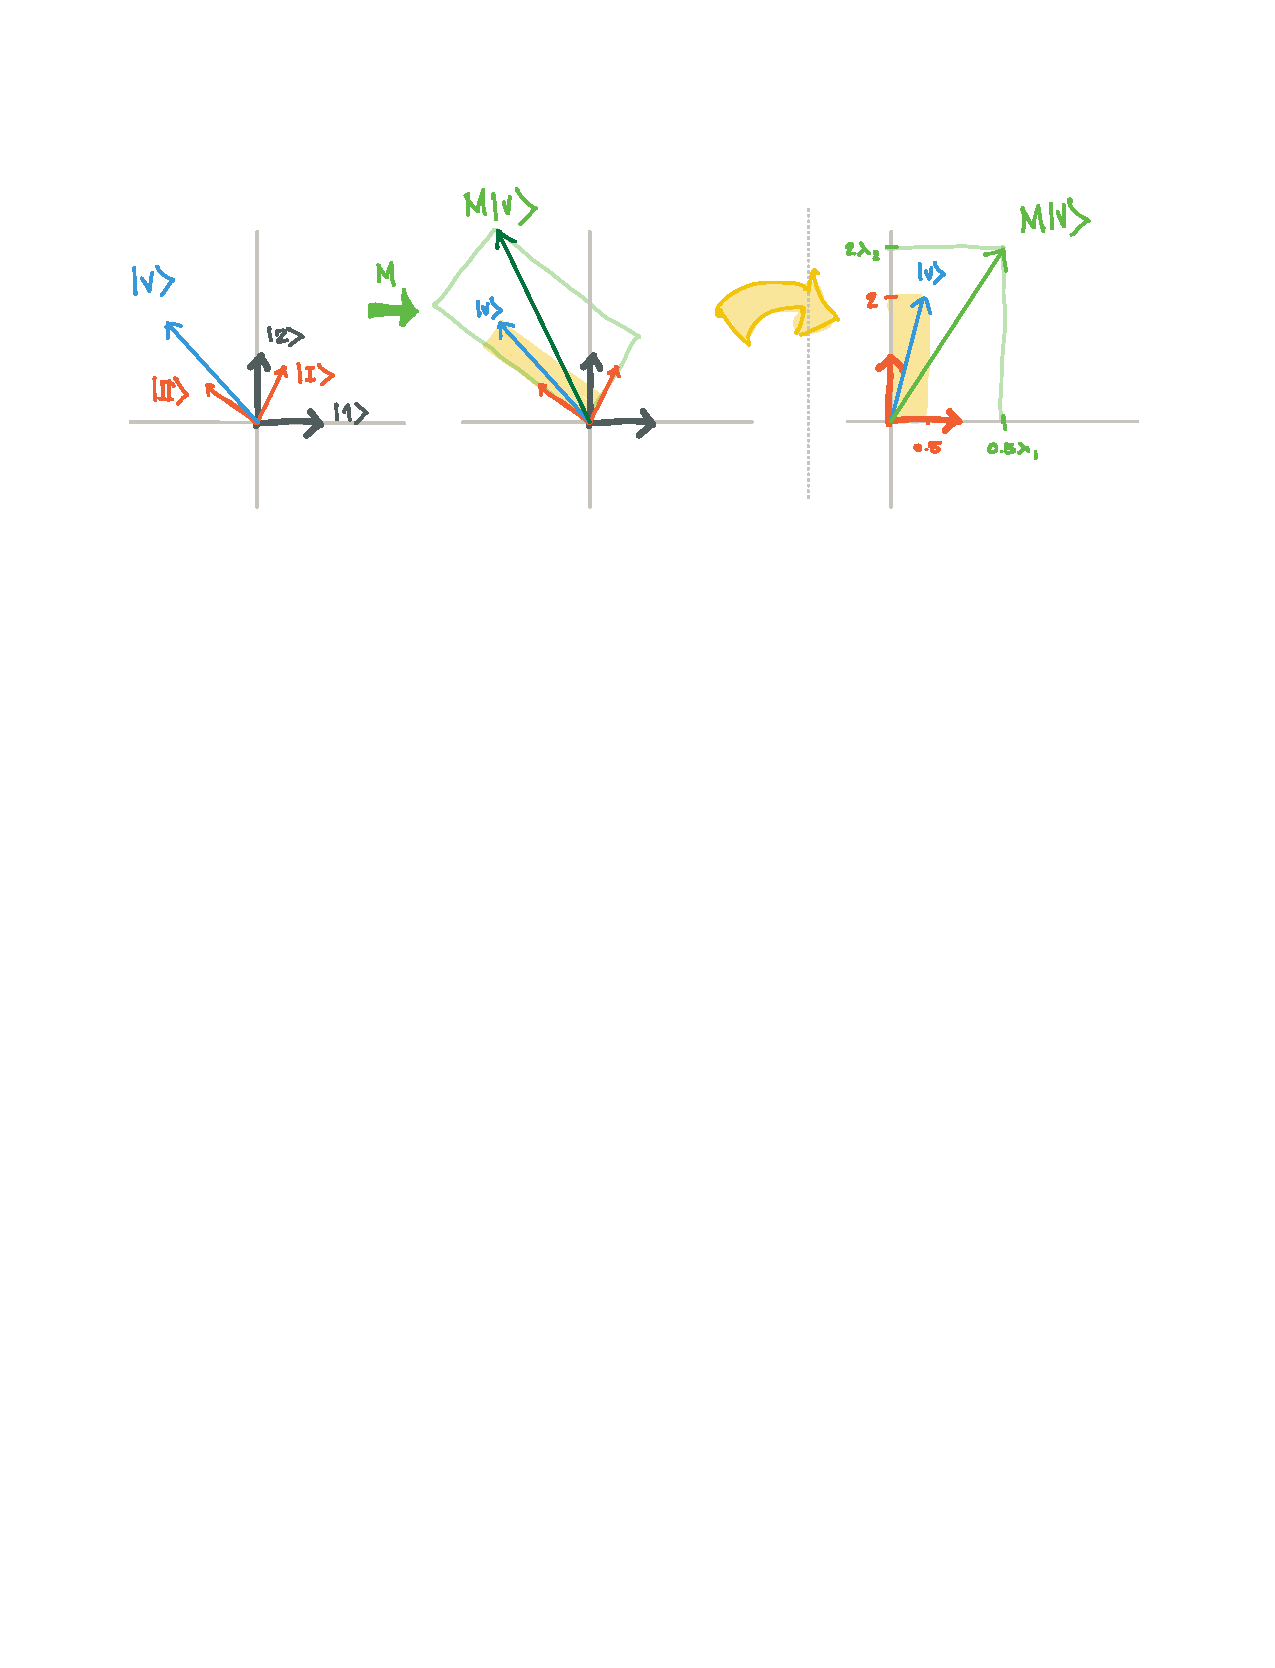
\includegraphics[width=.8\textwidth]{figures/eigen_transform.pdf}
    \caption{Standard basis (black) and eigenbasis (red) vectors and the vector $\ket{v}$ (blue) in \eqref{eq:eigen:example:v}. Under a transformation $M$, the vector is mapped to $M\ket{v}$ (green) which is a rescaling of the components of $\ket{v}$ along the eigenbasis directions (shown as a green box). Right: the transformation as seen by an eigen-observer's frame.}
    \label{fig:eigentransform}
\end{figure}

Passing to the eigenbasis gives a clear understanding of what a Hermitian linear transformation does. We sketch this in Figs.~\ref{fig:eigentransform} and \ref{fig:eigenbal}. For that example, we consider a matrix $M$ with eigenvectors $\ket{{\text{I},\text{II}}}$ and corresponding eigenvalues $\lambda_{\text{I},\text{II}}$:
\begin{align}
    M &= \begin{pmatrix}
        2 & 1 \\
        1 & 3
    \end{pmatrix}
    &
    \lambda_{\text{I},\text{II}} &\approx 3.6,\; 1.4 \ .
    &
    \ket{{\text{I},\text{II}}}&\approx
    \begin{pmatrix}
        0.5 \\ 0.9
    \end{pmatrix},
    \;
    \begin{pmatrix}
        -0.9 \ \\pp 0.5
    \end{pmatrix} \ .
\end{align}
Figure~\ref{fig:eigentransform} shows a vector 
\begin{align}
    \ket{v} = 0.5\ket{\text{I}} + 2\ket{\text{II}} \approx
    -1.4\ket{1} + 1.5 \ket{2} 
    \label{eq:eigen:example:v}
\end{align}
under the transformation $M$,
\begin{align}
    M\ket{v} = 0.5\lambda_\text{I}\ket{\text{I}} + 2 \lambda_\text{II}\ket{\text{II}} \approx
    -1.4\ket{1} + 3 \ket{2} \ .
    \label{eq:eigen:example:Mv}
\end{align}
What we see is that in the eigenbasis, $M$ simply \emph{rescales} the components of $\ket{v}$ along the eigenbasis directions. 


\begin{figure}[tb]
    \centering
    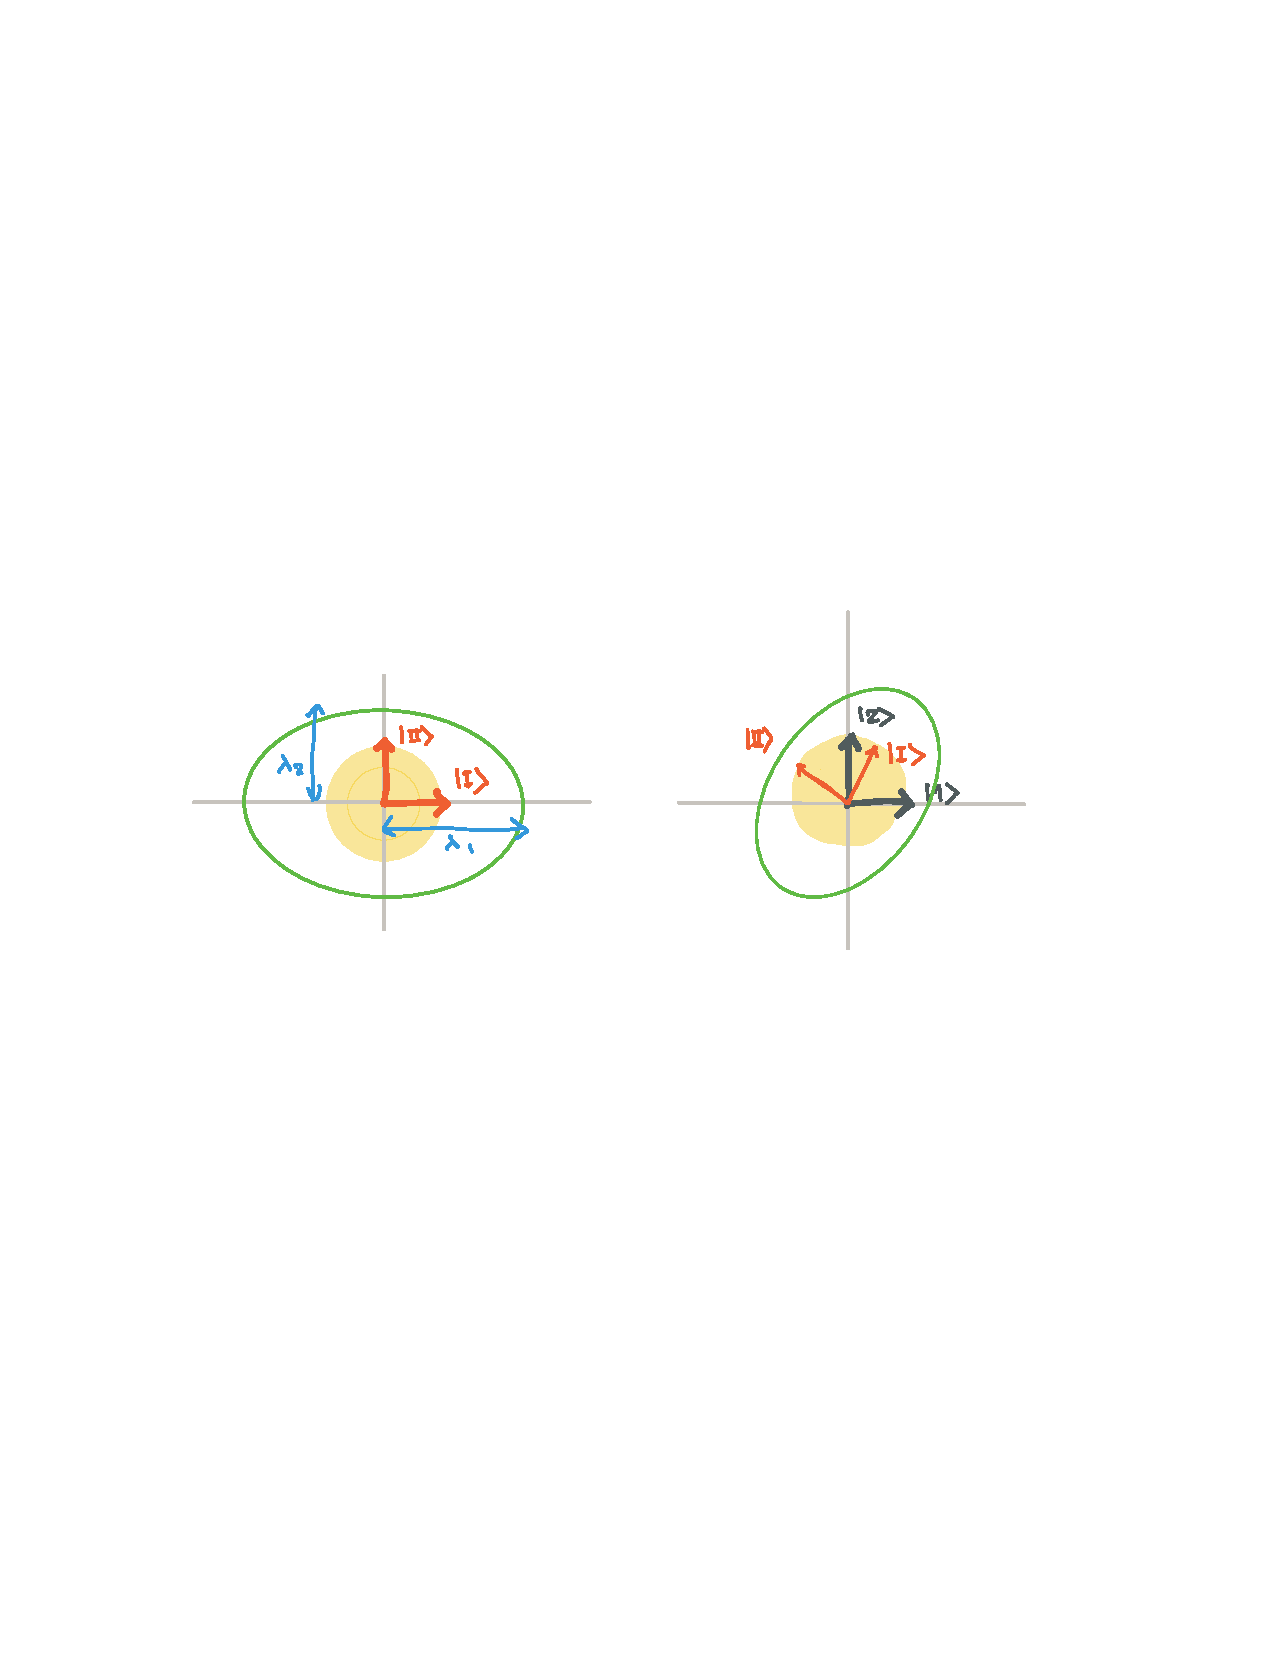
\includegraphics[width=.6\textwidth]{figures/eigen_ball.pdf}
    \caption{Eigenbasis directions are shown in red. The surface of the yellow ball represents all vectors of unit length. The green ellipse represents the deformation of this surface by acting on each of those vectors by $M$. We see that the eigenbasis components of these vectors are simply rescaled by the eigenvalues of $M$. Right: Same figure, but drawn relative to the standard basis.}
    \label{fig:eigenbal}
\end{figure}

Figure~\ref{fig:eigentransform} shows a unit ball in the eigenbasis and how it is deformed under $M$. The surface of the ball should be understood as endpoints of a set of possible vectors. Under $M$, this surface is deformed to the green ellipse. In the standard basis, this ellipse is skewed by the rotation between the two bases. 






\subsection{Degenerate Eigenvalues}
% commutators
% start with trivial example, diagonal 

Sometimes a matrix will have degenerate eigenvalues. This means that $\lambda_i = \lambda_{i+1}$ for some pair of eigenvalues. We continue to assume that the eigenvalues are all non-zero, as required for invertible (nice!) matrices.  Degenerate eigenvalues can lead to some curiosities when applying the `standard procedure' above...

\section{Quantum Mechanics}
% ``operator''

\section{Function Space}
% fourier



\appendix

\section{Things we did not get to}
\begin{itemize}
\item Tensor densities
\item Symmetries and Lie Groups
\item Other types of integral transforms
\item Hamiltonian Mechanics and the co-tangent space
\item Rotations in the $\partial x'/\partial x$ notation.
\item non-coordinate bases
% \item \url{https://www.reddit.com/r/math/comments/12yp3z2/do_tensors_outside_of_physics_transform_like_a/}
\end{itemize}




\section*{Acknowledgments}

\acro{PT}\ thanks the students of Physics 17 (Spring 2022, Spring 2023) for their feedback and patience.
%
% \acro{PT} is supported by the \acro{DOE} grant \acro{DE-SC}/0008541.
\acro{PT} is supported by a \acro{NSF CAREER} award (\#2045333).

%% Appendices
% \appendix


%% Bibliography
%\bibliographystyle{utcaps} 	% arXiv hyperlinks, preserves caps in title
%\bibliographystyle{utphys} 	% arXiv hyperlinks
% \bibliography{bib title without .bib}

\end{document}